% Options for packages loaded elsewhere
\PassOptionsToPackage{unicode}{hyperref}
\PassOptionsToPackage{hyphens}{url}
%
\documentclass[
]{krantz}
\usepackage{amsmath,amssymb}
\usepackage{lmodern}
\usepackage{iftex}
\ifPDFTeX
  \usepackage[T1]{fontenc}
  \usepackage[utf8]{inputenc}
  \usepackage{textcomp} % provide euro and other symbols
\else % if luatex or xetex
  \usepackage{unicode-math}
  \defaultfontfeatures{Scale=MatchLowercase}
  \defaultfontfeatures[\rmfamily]{Ligatures=TeX,Scale=1}
  \setmonofont[]{Source Code Pro}
\fi
% Use upquote if available, for straight quotes in verbatim environments
\IfFileExists{upquote.sty}{\usepackage{upquote}}{}
\IfFileExists{microtype.sty}{% use microtype if available
  \usepackage[]{microtype}
  \UseMicrotypeSet[protrusion]{basicmath} % disable protrusion for tt fonts
}{}
\makeatletter
\@ifundefined{KOMAClassName}{% if non-KOMA class
  \IfFileExists{parskip.sty}{%
    \usepackage{parskip}
  }{% else
    \setlength{\parindent}{0pt}
    \setlength{\parskip}{6pt plus 2pt minus 1pt}}
}{% if KOMA class
  \KOMAoptions{parskip=half}}
\makeatother
\usepackage{xcolor}
\IfFileExists{xurl.sty}{\usepackage{xurl}}{} % add URL line breaks if available
\IfFileExists{bookmark.sty}{\usepackage{bookmark}}{\usepackage{hyperref}}
\hypersetup{
  pdftitle={Improving Your Statistical Inferences},
  pdfauthor={Daniel Lakens},
  hidelinks,
  pdfcreator={LaTeX via pandoc}}
\urlstyle{same} % disable monospaced font for URLs
\usepackage{color}
\usepackage{fancyvrb}
\newcommand{\VerbBar}{|}
\newcommand{\VERB}{\Verb[commandchars=\\\{\}]}
\DefineVerbatimEnvironment{Highlighting}{Verbatim}{commandchars=\\\{\}}
% Add ',fontsize=\small' for more characters per line
\usepackage{framed}
\definecolor{shadecolor}{RGB}{248,248,248}
\newenvironment{Shaded}{\begin{snugshade}}{\end{snugshade}}
\newcommand{\AlertTok}[1]{\textcolor[rgb]{0.94,0.16,0.16}{#1}}
\newcommand{\AnnotationTok}[1]{\textcolor[rgb]{0.56,0.35,0.01}{\textbf{\textit{#1}}}}
\newcommand{\AttributeTok}[1]{\textcolor[rgb]{0.77,0.63,0.00}{#1}}
\newcommand{\BaseNTok}[1]{\textcolor[rgb]{0.00,0.00,0.81}{#1}}
\newcommand{\BuiltInTok}[1]{#1}
\newcommand{\CharTok}[1]{\textcolor[rgb]{0.31,0.60,0.02}{#1}}
\newcommand{\CommentTok}[1]{\textcolor[rgb]{0.56,0.35,0.01}{\textit{#1}}}
\newcommand{\CommentVarTok}[1]{\textcolor[rgb]{0.56,0.35,0.01}{\textbf{\textit{#1}}}}
\newcommand{\ConstantTok}[1]{\textcolor[rgb]{0.00,0.00,0.00}{#1}}
\newcommand{\ControlFlowTok}[1]{\textcolor[rgb]{0.13,0.29,0.53}{\textbf{#1}}}
\newcommand{\DataTypeTok}[1]{\textcolor[rgb]{0.13,0.29,0.53}{#1}}
\newcommand{\DecValTok}[1]{\textcolor[rgb]{0.00,0.00,0.81}{#1}}
\newcommand{\DocumentationTok}[1]{\textcolor[rgb]{0.56,0.35,0.01}{\textbf{\textit{#1}}}}
\newcommand{\ErrorTok}[1]{\textcolor[rgb]{0.64,0.00,0.00}{\textbf{#1}}}
\newcommand{\ExtensionTok}[1]{#1}
\newcommand{\FloatTok}[1]{\textcolor[rgb]{0.00,0.00,0.81}{#1}}
\newcommand{\FunctionTok}[1]{\textcolor[rgb]{0.00,0.00,0.00}{#1}}
\newcommand{\ImportTok}[1]{#1}
\newcommand{\InformationTok}[1]{\textcolor[rgb]{0.56,0.35,0.01}{\textbf{\textit{#1}}}}
\newcommand{\KeywordTok}[1]{\textcolor[rgb]{0.13,0.29,0.53}{\textbf{#1}}}
\newcommand{\NormalTok}[1]{#1}
\newcommand{\OperatorTok}[1]{\textcolor[rgb]{0.81,0.36,0.00}{\textbf{#1}}}
\newcommand{\OtherTok}[1]{\textcolor[rgb]{0.56,0.35,0.01}{#1}}
\newcommand{\PreprocessorTok}[1]{\textcolor[rgb]{0.56,0.35,0.01}{\textit{#1}}}
\newcommand{\RegionMarkerTok}[1]{#1}
\newcommand{\SpecialCharTok}[1]{\textcolor[rgb]{0.00,0.00,0.00}{#1}}
\newcommand{\SpecialStringTok}[1]{\textcolor[rgb]{0.31,0.60,0.02}{#1}}
\newcommand{\StringTok}[1]{\textcolor[rgb]{0.31,0.60,0.02}{#1}}
\newcommand{\VariableTok}[1]{\textcolor[rgb]{0.00,0.00,0.00}{#1}}
\newcommand{\VerbatimStringTok}[1]{\textcolor[rgb]{0.31,0.60,0.02}{#1}}
\newcommand{\WarningTok}[1]{\textcolor[rgb]{0.56,0.35,0.01}{\textbf{\textit{#1}}}}
\usepackage{longtable,booktabs,array}
\usepackage{calc} % for calculating minipage widths
% Correct order of tables after \paragraph or \subparagraph
\usepackage{etoolbox}
\makeatletter
\patchcmd\longtable{\par}{\if@noskipsec\mbox{}\fi\par}{}{}
\makeatother
% Allow footnotes in longtable head/foot
\IfFileExists{footnotehyper.sty}{\usepackage{footnotehyper}}{\usepackage{footnote}}
\makesavenoteenv{longtable}
\usepackage{graphicx}
\makeatletter
\def\maxwidth{\ifdim\Gin@nat@width>\linewidth\linewidth\else\Gin@nat@width\fi}
\def\maxheight{\ifdim\Gin@nat@height>\textheight\textheight\else\Gin@nat@height\fi}
\makeatother
% Scale images if necessary, so that they will not overflow the page
% margins by default, and it is still possible to overwrite the defaults
% using explicit options in \includegraphics[width, height, ...]{}
\setkeys{Gin}{width=\maxwidth,height=\maxheight,keepaspectratio}
% Set default figure placement to htbp
\makeatletter
\def\fps@figure{htbp}
\makeatother
\setlength{\emergencystretch}{3em} % prevent overfull lines
\providecommand{\tightlist}{%
  \setlength{\itemsep}{0pt}\setlength{\parskip}{0pt}}
\setcounter{secnumdepth}{5}
\newlength{\cslhangindent}
\setlength{\cslhangindent}{1.5em}
\newlength{\csllabelwidth}
\setlength{\csllabelwidth}{3em}
\newlength{\cslentryspacingunit} % times entry-spacing
\setlength{\cslentryspacingunit}{\parskip}
\newenvironment{CSLReferences}[2] % #1 hanging-ident, #2 entry spacing
 {% don't indent paragraphs
  \setlength{\parindent}{0pt}
  % turn on hanging indent if param 1 is 1
  \ifodd #1
  \let\oldpar\par
  \def\par{\hangindent=\cslhangindent\oldpar}
  \fi
  % set entry spacing
  \setlength{\parskip}{#2\cslentryspacingunit}
 }%
 {}
\usepackage{calc}
\newcommand{\CSLBlock}[1]{#1\hfill\break}
\newcommand{\CSLLeftMargin}[1]{\parbox[t]{\csllabelwidth}{#1}}
\newcommand{\CSLRightInline}[1]{\parbox[t]{\linewidth - \csllabelwidth}{#1}\break}
\newcommand{\CSLIndent}[1]{\hspace{\cslhangindent}#1}
\usepackage{booktabs}

\usepackage{booktabs}
\usepackage{longtable}
\usepackage{array}
\usepackage{multirow}
\usepackage{wrapfig}
\usepackage{float}
\usepackage{colortbl}
\usepackage{pdflscape}
\usepackage{tabu}
\usepackage{threeparttable}
\usepackage{threeparttablex}
\usepackage[normalem]{ulem}
\usepackage{makecell}
\usepackage{xcolor}
\ifLuaTeX
  \usepackage{selnolig}  % disable illegal ligatures
\fi
\usepackage[]{natbib}
\bibliographystyle{apalike}

\title{Improving Your Statistical Inferences}
\author{Daniel Lakens}
\date{2022-03-03}

\begin{document}
\maketitle

{
\setcounter{tocdepth}{1}
\tableofcontents
}
\hypertarget{welcome}{%
\chapter*{Welcome}\label{welcome}}
\addcontentsline{toc}{chapter}{Welcome}

This open educational resource integrates information from my \href{https://daniellakens.blogspot.com/}{blog}, my MOOCs \href{https://www.coursera.org/learn/statistical-inferences}{Improving Your Statistical Inferences} and \href{https://www.coursera.org/learn/improving-statistical-questions}{Improving Your Statistical Questions}, and my \href{https://scholar.google.nl/citations?user=ZbqYyrsAAAAJ\&hl=en}{scientific work} in one place. The goal is to make the information findable, accessible, and make it easier to update the material based on recent scientific developments and new statistical software.

I have used my right to re-use and adapt my own open access articles, without adding quotation marks or citing myself. This work is shared under a \href{https://creativecommons.org/licenses/by-nc-nd/4.0/}{Creative Commons Attribution-NonCommercial-NoDerivatives 4.0 International License}. Thanks to my collaborators Casper Albers, Farid Anvari, Aaron Caldwell, Harlan Cambell, Nicholas Coles, Lisa DeBruine, Marie Delacre, Zoltan Dienes, Noah van Dongen, Alexander Etz, Ellen Evers, Jaroslav Gottfriend, Seth Green, Christopher Harms, Arianne Herrera-Bennett, Joe Hilgard, Peder Isager, Maximilian Maier, Neil McLatchie, Brian Nosek, Pepijn Obels, Amy Orben, Anne Scheel, Janneke Staaks, Leo Tiokhin, Mehmet Tunç, Duygu Uygun Tunç, who have contributed to the work I have done in the past that has in part formed the basis of this material.

If you find any mistakes, or have suggestions for improvement, you can \href{https://github.com/Lakens/statistical_inferences/issues}{submit an issue on the GitHub page} of this open educational resource. I hope this material will be of use to you.

Dr.~Daniël Lakens

\begin{center}
\includegraphics[width=0.3\linewidth]{images/me} \end{center}

\hypertarget{pvalue}{%
\chapter{\texorpdfstring{Using \emph{p}-values to test a hypothesis}{Using p-values to test a hypothesis}}\label{pvalue}}

One question that interests scientists is whether differences exist on measurements that have been collected under different conditions. The answer to such a question is an \emph{ordinal claim}. For example, a researcher might hypothesize that some of the time students spend on learning new information should be dedicated to the retrieval of information by doing tests (condition A), compared to spending all of the time studying (condition B). After collecting data, and observing that the mean grade is higher for students in for student who spend part of their time doing tests, the researcher can make the ordinal claim that student performence was better in condition A than in condition B. Ordinal claims do not quantify the \textbf{size of the effect}. Ordinal claims can only be used to state there is a difference between conditions. In a \emph{non-directional} (or \emph{two-sided}) test the question is whether there is a difference in either direction, and in a directional (or \emph{one-sided}) test the question is whether there is an effect in a specific direction, with in both cases the alternative being that there is no such difference.

To make ordinal claims, researchers typically rely on a methodological procedure known as a \textbf{hypothesis test}. One part of a hypothesis test consists of computing a \textbf{p-value} and examining whether there is a statistically \textbf{significant} difference. `Significant' means that something is worthy of attention. A hypothesis test is used to distinguish a signal (that is worth paying attention to) from random noise in empirical data. It is worth distinguishing \textbf{statistical significance}, which is only used to claim whether an observed effect is a signal or noise, from \textbf{practical significance}, which depends on whether the size of the effect is large enough to have any worthwhile consequences in real life. The use of a methodological procedure to decide whether an ordinal claim can be made functions as a safeguard against confirmation bias. Depending on their desires, scientists might be tempted to interpret data as support for their hypothesis, even when it is not. A hypothesis test, when used correctly, controls the amount of time researchers will fool themselves when they make ordinal claims.

\hypertarget{philosophical-approaches-to-p-values}{%
\section{\texorpdfstring{Philosophical approaches to \emph{p}-values}{Philosophical approaches to p-values}}\label{philosophical-approaches-to-p-values}}

Before we look at how p-values are computed, it is important to examine how they are supposed to help us make ordinal claims when testing hypotheses. The definition of a \emph{p}-value is the probability of observing the sample data, or more extreme data, assuming the null hypothesis is true. But this definition does not tell us much about how we should interpret a \emph{p}-value.

The interpretation of a \emph{p}-value depends on the statistical philosophy one subscribes to. \href{https://en.wikipedia.org/wiki/Ronald_Fisher}{Ronald Fisher} published `Statistical Methods for Research Workers' in 1925 which popularized \emph{p}-values. In a Fisherian framework a \emph{p}-value is interpreted as a descriptive continuous measure of compatibility between the observed data and the null-hypothesis \citep{greenland_statistical_2016}. The compatibility of observed data with the null model falls between 1 (perfectly compatible) and 0 (extremely incompatible), and every individual can interpret the \emph{p}-value with ``statistical thoughtfulness''. According to Fisher \citeyearpar{fisher_statistical_1956}, p-values ``do not generally lead to any probability statement about the real world, but to a rational and well-defined measure of the reluctance to accept the hypotheses they test''. Fisher tried to formalize his philosophy in an approach called `fiducial inference', but this has not recevied the same widespread adoption of other approaches, such as decision theory, likelihoods, and Bayesian inference. Indeed, Zabell \citeyearpar{zabell_r_1992} writes ``The fiducial argument stands as Fisher's one great failure'', although others have expressed the hope that it might be developed into a useful approach in the future \citep{schweder_confidence_2016}. A Fisherian \emph{p}-value describes the incompatibility of the data with a single hypothesis, and is known as \emph{significance testsing}. The main reason a \emph{significance test} is so limited, is because researchers only have to specify a null-hypothesis, but they do not have to specify an alternative hypothesis.

Neyman and Pearson built on insights about \emph{p}-values by William Gosset (the inventor of the Student's \emph{t}-test) and Ronald Fisher, and developed an approached called \emph{statistical hypothesis testing}. The main difference with the significance testing approach developed by Fisher was that in a statistical hypothesis test both a null-hypothesis and an alternative hypothesis is specified. In a Neyman-Pearson framework the goal of statistical tests is to guide the behavior of researchers with respect to these two hypotheses. Based on the results of a statistical test, and without ever knowing whether the hypothesis is true or not, researchers choose to tentatively act as if the null hypothesis or the alternative hypothesis is true. In psychology, researchers often use an imperfect hybrid of the Fisherian and Neyman-Pearson frameworks, but the Neyman-Pearson approach is, according to Dienes \citet{dienes_understanding_2008} ``the logic underlying all the statistics you see in the professional journals of psychology''.

When a Neyman-Pearson hypothesis test is performed the observed \emph{p}-value is only used to check if it is smaller than the chosen alpha level, but it does not matter how much smaller it is. For example, if an alpha level of 0.01 is used, both a \emph{p} = 0.006 and a \emph{p} = 0.000001 lead the researchers to decide to act as if the state of the world is best described by the alternative hypothesis. This differs from a Fisherian approach to \emph{p}-values, where the lower the \emph{p}-value, the greater the psychological reluctance of a researcher to accept the null-hypothesis they are testing. A Neyman-Pearson hypothesis test does not see the goal of an inference as quantifying a continuous measure of compatibility or evidence. Instead, as Neyman \citeyearpar{neyman_inductive_1957} writes:

\begin{quote}
The content of the concept of inductive behavior is the recognition that the purpose of every piece of serious research is to provide grounds for the selection of one of several contemplated courses of action.
\end{quote}

Intuitively, one might feel like decisions about how to act should not be based on the results of a single statistical test, and this point is often raised as a criticism of a Neyman-Pearson approach to statistical inferences. However, such criticisms rarely use the same definition of an `act' as Neyman used. It is true that, for example, the decision to implement a new government policy should not be based on a single study result. However, Neyman considered making a scientific claim an `act' as well, and wrote (1957, p.~10) that the concluding phase of a study involves:

\begin{quote}
an act of will or a decision to take a particular action, perhaps to assume a particular attitude towards the various sets of hypotheses
\end{quote}

Cox \citeyearpar{cox_problems_1958} writes:

\begin{quote}
it might be argued that in making an inference we are `deciding' to make a statement of a certain type about the populations and that therefore, provided that the word decision is not interpreted too narrowly, the study of statistical decisions embraces that of inference. The point here is that one of the main general problems of statistical inference consists in deciding what types of statement can usefully be made and exactly what they mean.
\end{quote}

Thus, in a Neyman-Pearson approach, \emph{p}-values form the basis of decisions about which claims to make. In science, such claims underly most novel experiments in the form of \textbf{auxiliary hypotheses}, or the assumptions about underlying hypotheses that are assumed to be accurate in order for a test to work as planned. For example, if it is important that participants can see color in a planned experiment, we assume it is true that the \href{https://en.wikipedia.org/wiki/Ishihara_test}{Ishihara test} successfully identifies which participants are colorblind.

\hypertarget{creating-a-null-model}{%
\section{Creating a null model}\label{creating-a-null-model}}

\begin{figure}

{\centering 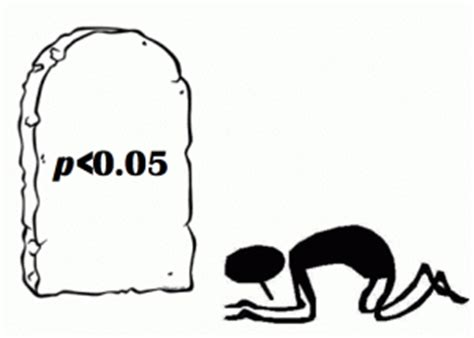
\includegraphics[width=0.25\linewidth]{images/worship} 

}

\caption{Scientists have a tendency to worship *p*-values below a value of 0.05.}\label{fig:worship}
\end{figure}

Assume I ask two groups of 10 people how much they liked the extended directors cut of the Lord of the Rings (LOTR) trilogy. This means our \textbf{total sample size} (\emph{N}) is 20, and the sample size in each group (\emph{n}) is 10. The first group consists of my friends, and the second groups consists of friends of my wife. Our friends rate the trilogy on a score from 1 to 10. We can calculate the average rating by my friends, which is 8.7, and the average rating by my wife's friends, which is 7.7. We can compare the scores in both groups by looking at the raw data, and by plotting the data.

\begin{table}

\caption{\label{tab:friends}Ratings for the Lord of the Rings extended trilogy by two groups of friends.}
\begin{tabular}[t]{lcc}
\toprule
 & Friends Daniel & Friends Kyra\\
\midrule
friend\_1 & 9 & 9\\
friend\_2 & 7 & 6\\
friend\_3 & 8 & 7\\
friend\_4 & 9 & 8\\
friend\_5 & 8 & 7\\
\addlinespace
friend\_6 & 9 & 9\\
friend\_7 & 9 & 8\\
friend\_8 & 10 & 8\\
friend\_9 & 9 & 8\\
friend\_10 & 9 & 7\\
\bottomrule
\end{tabular}
\end{table}

\begin{center}\includegraphics[width=1\linewidth]{01-pvalue_files/figure-latex/unnamed-chunk-3-1} \end{center}

We can see the groups overlap but the mean ratings differ by 1 whole point. The question we are no faced with is the following: Is the difference between the two groups just random variation, or can we claim that my friends like the extended directors cut of the Lord of the Rings (LOTR) trilogy more than my wife's friends?

In a \textbf{null-hypothesis significance test} we try to answer this question by calculating the probability of the observed difference (in this case, a mean difference of 1) or a more extreme difference, under the assumption that there is no real difference between how much my friends and my wife's friends like the extended directors cut of LOTR, and we are just looking at random noise. This probability is called the \emph{p}-value. If this probability is low enough, we decide to claim there is a difference. If this probability is not low enough, we refrain from making a claim about a difference.

The null-hypothesis assumes that if we would ask an infinite number of my friends and an infinite number of my wife's friends how much they like LOTR, the difference between these huge groups is exactly 0. However, in any sample drawn draw from the population, random variation is very likely to lead to a difference somewhat larger or smaller than 0. We can create a \textbf{null model} that quantifies the expected variation in the observed data, just due to random noise, to tell us what constitutes a reasonable expectation about how much the differences between groups can vary if there is no difference in the population.

It is practical to create a null model in terms of a \textbf{standardized} distribution, as this makes it easier to calculate the probability that specific values will occur, regardless of the scale that is used to collect the measurements. One version of a null model for differences is the \emph{t}-distribution, which can be used to describe which differences should be expected when drawing samples from a population. Such a null model is built on \textbf{assumptions}. In the case of the \emph{t}-distribution, the assumption is that scores are normally distributed. In reality, the assumptions upon which statistical methods are built are never met perfectly, which is why statisticians examine the impact of violations of assumptions on methodological procedures. Statistical tests are still useful in practice when the impact of violations on statistical inferences is small enough.

We can quantify the distribution of \emph{t}-values that is expected when there is no difference in the population by a \emph{probability density function}. Below is a plot of the probability density function for a \emph{t}-distribution with 18 \textbf{degrees of freedom} (df), which corresponds to our example where we collect data from 20 friends (df = N - 2 for two independent groups). For a continuous distribution, where probabilities are defined for an infinite number of points, the probability of observing any single point (e.g., \emph{t} = 2.5) is always zero. Probabilities are measured over intervals. For this reason, when a \emph{p}-value is computed, it is not defined as `the probability of observing the data', but as `the probability of observed the data, \emph{or more extreme data}'. This creates an interval (a tail of a distribution) for which a probability can be calculated.

\hypertarget{calculating-a-p-value}{%
\section{\texorpdfstring{Calculating a \emph{p}-value}{Calculating a p-value}}\label{calculating-a-p-value}}

A \emph{t}-value can be computed from the mean in the sample, the mean in the population, the standard deviation in the sample, and the sample size. By then computing the probability of observing a \emph{t}-value as extreme or more extreme as the one observed, we get a \emph{p}-value. For the comparison of the movie ratings for the two groups of friends above, performing a two-sided Student's \emph{t}-test yields a \emph{t}-value of 2.5175 and a \emph{p}-value of 0.02151.

\begin{Shaded}
\begin{Highlighting}[]
\FunctionTok{t.test}\NormalTok{(df\_long}\SpecialCharTok{$}\NormalTok{rating }\SpecialCharTok{\textasciitilde{}}\NormalTok{ df\_long}\SpecialCharTok{$}\StringTok{\textasciigrave{}}\AttributeTok{Friend Group}\StringTok{\textasciigrave{}}\NormalTok{, }\AttributeTok{var.equal =} \ConstantTok{TRUE}\NormalTok{)}
\end{Highlighting}
\end{Shaded}

\begin{verbatim}
## 
##  Two Sample t-test
## 
## data:  df_long$rating by df_long$`Friend Group`
## t = 2.5175, df = 18, p-value = 0.02151
## alternative hypothesis: true difference in means between group Friends Daniel and group Friends Kyra is not equal to 0
## 95 percent confidence interval:
##  0.1654875 1.8345125
## sample estimates:
## mean in group Friends Daniel   mean in group Friends Kyra 
##                          8.7                          7.7
\end{verbatim}

We can graph the \emph{t}-distribution (for df = 18) and highlight the two tail areas that start at the t-values of 2.5175 and -2.5175.

\begin{figure}

{\centering 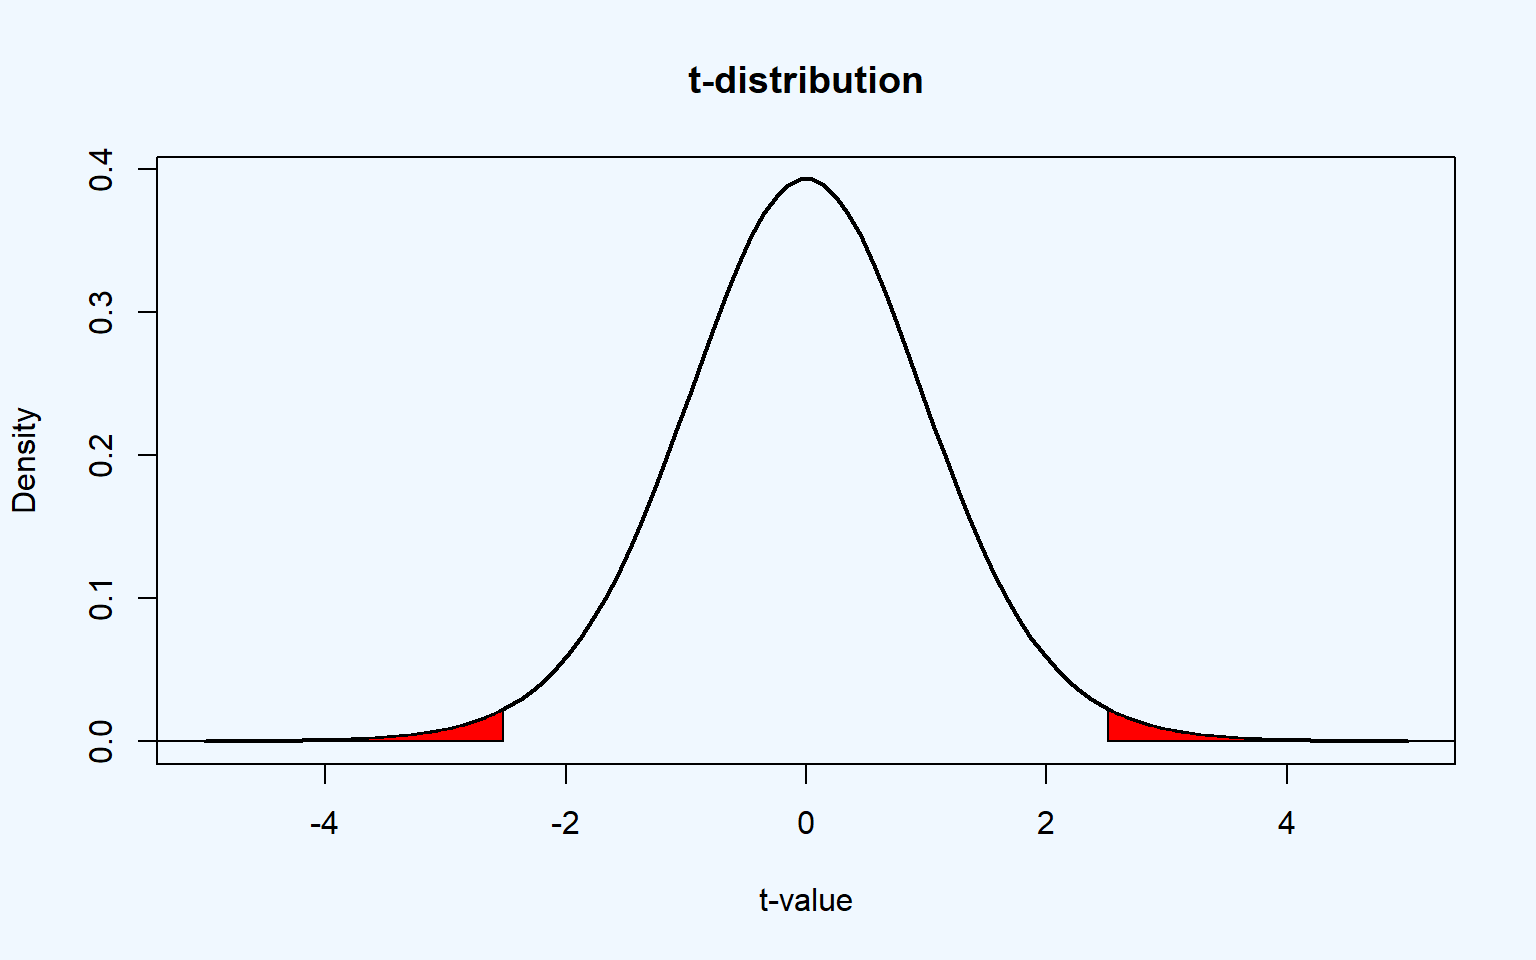
\includegraphics[width=1\linewidth]{01-pvalue_files/figure-latex/tdist-1} 

}

\caption{A *t*-distribution with 18 degrees of freedom.}\label{fig:tdist}
\end{figure}

\hypertarget{which-p-values-can-you-expect}{%
\section{\texorpdfstring{Which \emph{p}-values can you expect?}{Which p-values can you expect?}}\label{which-p-values-can-you-expect}}

In a very educational video about the `\href{https://www.youtube.com/watch?v=5OL1RqHrZQ8}{Dance of the \emph{p}-values}', Geoff Cumming explains that \emph{p}-values vary from experiment to experiment. However, this is not a reason to `not trust p' as he mentions in the video. Instead, it is important to clearly understand \textbf{\emph{p}-value distributions} to prevent misconceptions. Because \emph{p}-values are part of frequentist statistics, we need to examine what we can expect \emph{in the long run}. Because we never do the same experiment hundreds of times, and we do only a very limited number of studies in our lifetime, the best way to learn about what we should expect in the long run is through computer simulations.

Take a moment to try to answer the following two questions. Which \emph{p}-values can you expect to observe if there is a true effect, and you repeat the same study one-hundred thousand times? And which \emph{p}-values can you expect if there is no true effect, and you repeat the same study one-hundred thousand times? If you don't know the answer, don't worry - you will learn it now. But if you don't know the answer, it is worth reflecting on why you don't know the answer about such an essential aspect of \emph{p}-values. If you are like me, you were simply never taught this. But as we will see, it is essential to a solid understanding of how to interpret \emph{p}-values.

Which \emph{p}-values you can expect is completely determined by the statistical power of the study, or the probability that you will observe a significant effect, if there is a true effect. The statistical power ranges from 0 to 1. We can illustrate this by simulating one-sample \emph{t}-tests. The idea is that we simulate IQ scores for a group of people. We know the standard deviation of IQ scores is 15. For now, we will set the mean IQ score in the simulated group to 106, which we will compare to the average IQ score of all people (which is known to be 100 -- that's how IQ tests are normalized). We are testing if the people in our simulated sample have an IQ that differs from the average (and we know the correct answer is `yes', because we made it so in the simulation).

\begin{Shaded}
\begin{Highlighting}[]
\NormalTok{p }\OtherTok{\textless{}{-}} \FunctionTok{numeric}\NormalTok{(}\DecValTok{100000}\NormalTok{) }\CommentTok{\# store all simulated *p*{-}values}

\ControlFlowTok{for}\NormalTok{ (i }\ControlFlowTok{in} \DecValTok{1}\SpecialCharTok{:}\DecValTok{100000}\NormalTok{) \{ }\CommentTok{\# for each simulated experiment}
\NormalTok{  x }\OtherTok{\textless{}{-}} \FunctionTok{rnorm}\NormalTok{(}\AttributeTok{n =} \DecValTok{71}\NormalTok{, }\AttributeTok{mean =} \DecValTok{100}\NormalTok{, }\AttributeTok{sd =} \DecValTok{15}\NormalTok{) }\CommentTok{\# Simulate data}
\NormalTok{  y }\OtherTok{\textless{}{-}} \FunctionTok{rnorm}\NormalTok{(}\AttributeTok{n =} \DecValTok{71}\NormalTok{, }\AttributeTok{mean =} \DecValTok{105}\NormalTok{, }\AttributeTok{sd =} \DecValTok{15}\NormalTok{) }\CommentTok{\# Simulate data}
\NormalTok{  p[i] }\OtherTok{\textless{}{-}} \FunctionTok{t.test}\NormalTok{(x, y)}\SpecialCharTok{$}\NormalTok{p.value }\CommentTok{\# store the *p*{-}value}
\NormalTok{\}}

\NormalTok{(}\FunctionTok{sum}\NormalTok{(p }\SpecialCharTok{\textless{}} \FloatTok{0.05}\NormalTok{) }\SpecialCharTok{/} \DecValTok{100000}\NormalTok{) }\CommentTok{\# compute power}
\FunctionTok{hist}\NormalTok{(p, }\AttributeTok{breaks =} \DecValTok{20}\NormalTok{) }\CommentTok{\# plot a histogram}
\end{Highlighting}
\end{Shaded}

In the simulation, we generate n = 71 normally distributed IQ scores with a mean of M (106 by default) and a standard deviation of 15. We then perform a one-sample \emph{t}-test and store the \emph{p}-value. If we would plot the distribution of

\textbackslash begin\{figure\}

\{\centering 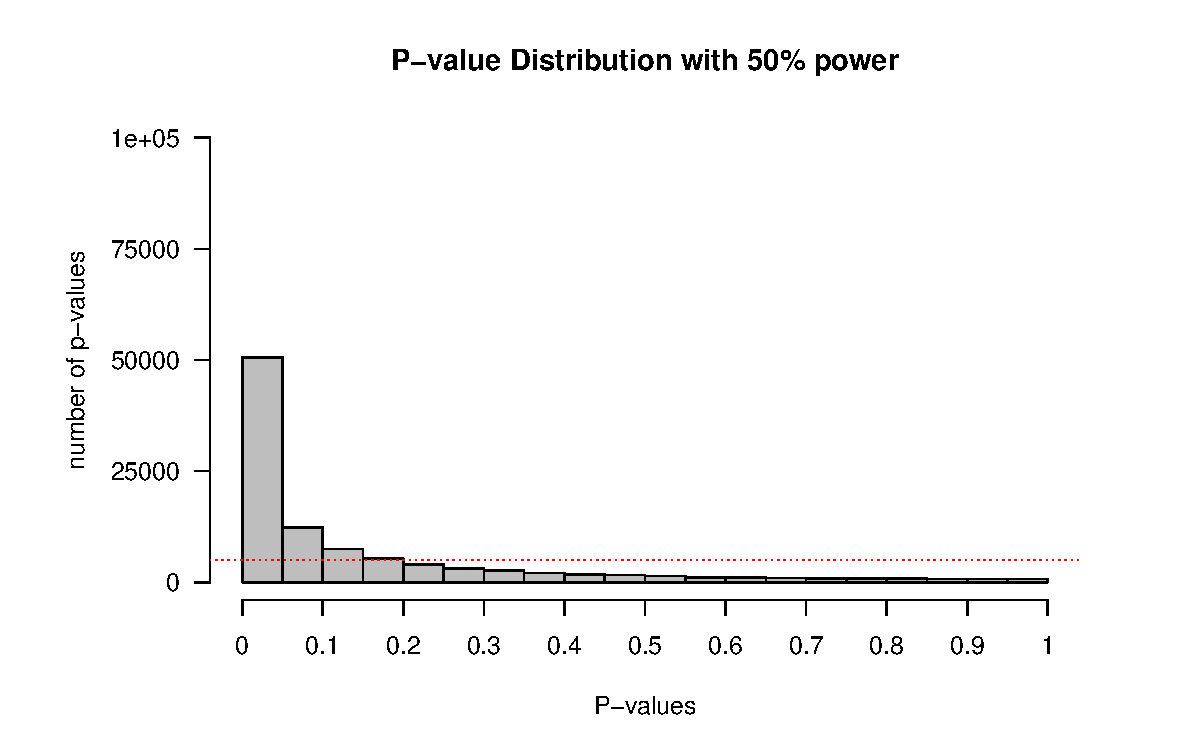
\includegraphics[width=1\linewidth]{01-pvalue_files/figure-latex/pdistr1-1}

\}

\textbackslash caption\{Distribution of \emph{p}-values when power = 50\%.\}\label{fig:pdistr1}
\textbackslash end\{figure\}

On the x-axis we see \emph{p}-values from 0 to 1 in 20 bars, and on the y-axis we see how frequently these \emph{p}-values were observed. There is a horizontal red dotted line that indicates an alpha of 5\% (located at a frequency of 100.000*0.05 = 5000) -- but you can ignore this line for now. In the title of the graph, the statistical power that is achieved in the simulated studies is given (assuming an alpha of 0.05): The studies have 50\% power.

The simulation result illustrates the \textbf{probability density function} of \emph{p}-values. A probability density function provides the probability that a random variable has a specific value (such as Figure \ref{fig:tdist} of the \emph{t}-distribution). Because the \emph{p}-value is a random variable, we can use it's probability density function to plot the \emph{p}-value distribution \citep{hung_behavior_1997, ulrich_properties_2018}, as in Figure \ref{fig:pdft}. You can vary the sample size, effect size, and alpha level in \href{http://shiny.ieis.tue.nl/d_p_power/}{this online Shiny app}. Increasing the sample size or the effect size will increase the steepness of the \emph{p}-value distribution, which means that the probability to observe small \emph{p}-values increases. The \emph{p}-value distribution is a function of the statistical power of the test.

\begin{figure}

{\centering 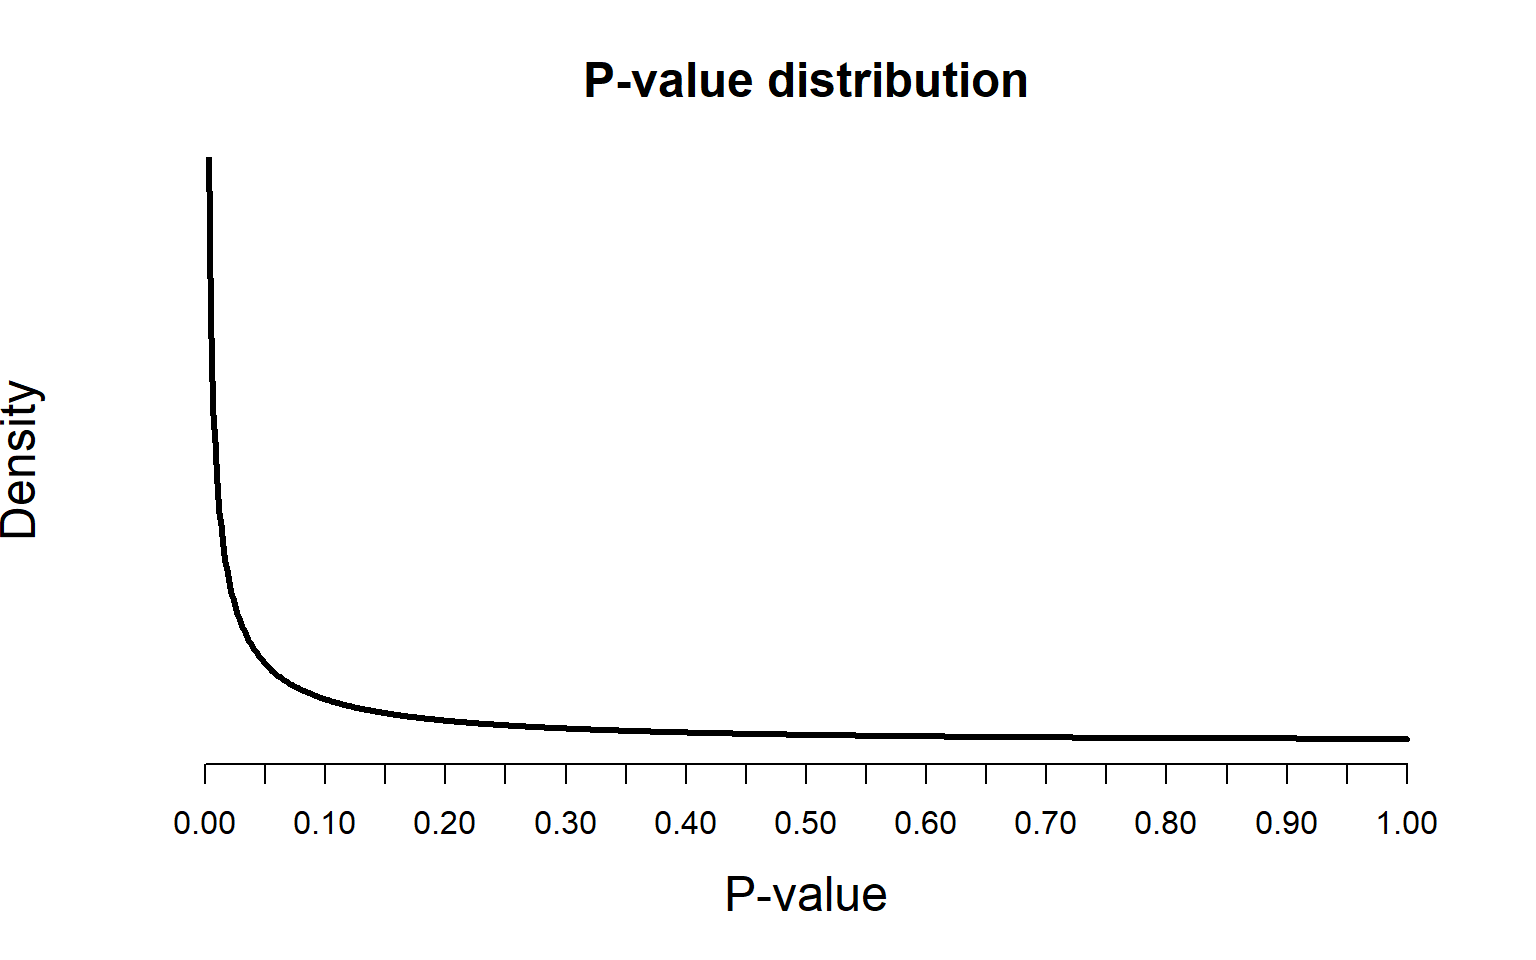
\includegraphics[width=1\linewidth]{01-pvalue_files/figure-latex/pdft-1} 

}

\caption{Probability density function for p-values from a two-sided t-test.}\label{fig:pdft}
\end{figure}

When there is no true effect, \emph{p}-values are \textbf{uniformly distributed}. This means that every \emph{p}-value is equally likely to be observed when the null hypothesis is true. In other words, when there is no true effect, a \emph{p}-value of 0.08 is just as likely as a \emph{p}-value of 0.98. I remember thinking this was very counterintuitive when I first learned it (well after completing a PhD), but it makes sense when we think of the goal to guarantee that when H0 is true, alpha \% of the \emph{p}-values fall below the alpha level. If we set alpha to 0.01, 1\% of the observed \emph{p}-values should fall below 0.01, and if we set alpha to 0.12, 12\% of the observed \emph{p}-values should fall below 0.12. This can only happen if \emph{p}-values are uniformly distributed when the null-hypothesis is true.

\textbackslash begin\{figure\}

\{\centering 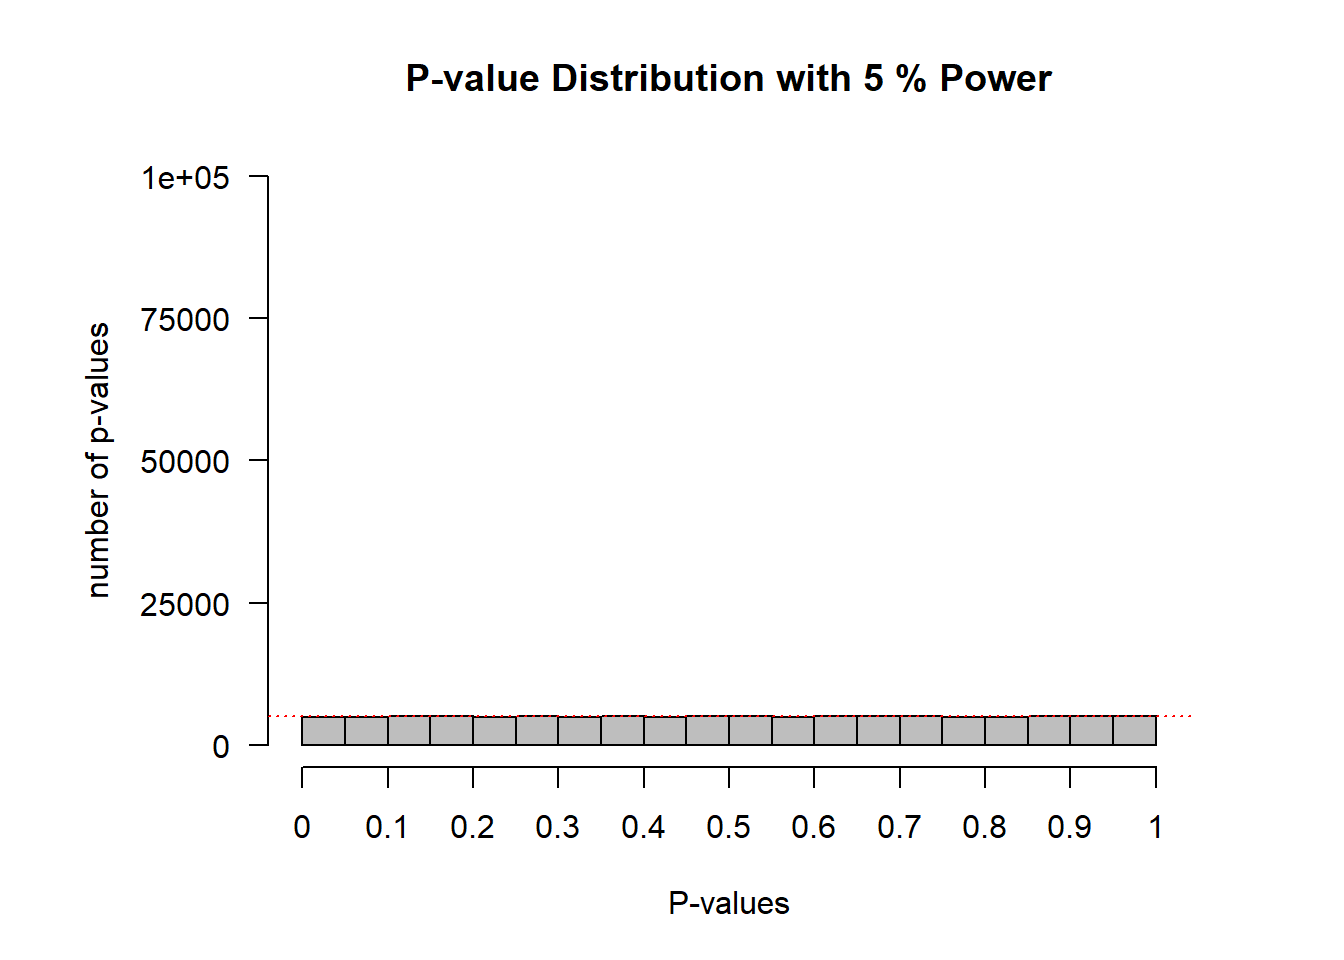
\includegraphics[width=1\linewidth]{01-pvalue_files/figure-latex/pdistr2-1}

\}

\textbackslash caption\{Distribution of \emph{p}-values when power = 50\%.\}\label{fig:pdistr2}
\textbackslash end\{figure\}

\hypertarget{lindley}{%
\section{Lindley's paradox}\label{lindley}}

As the statistical power increases, some \emph{p}-values below 0.05 (e.g., \emph{p} = 0.04) can be more likely when there is \emph{no} effect than when there \emph{is} an effect. This is known as Lindley's paradox \citep{lindley_statistical_1957}, or sometimes the Jeffreys-Lindley paradox \citep{spanos_who_2013}. Because the distribution of \emph{p}-values is a function of the statistical power \citep{cumming_replication_2008}, the higher the power, the more right-skewed the distribution becomes (i.e., the more likely it becomes that small \emph{p}-values are observed). When there is no true effect \emph{p}-values are uniformly distributed, and 1\% of observed \emph{p}-values fall between 0.04 and 0.05. When the statistical power is extremely high, not only will most \emph{p}-values fall below 0.05, most \emph{p}-values will fall below 0.01. In Figure \ref{fig:paradox} we see that with high power very small \emph{p}-values (e.g., 0.001) are more likely to be observed when there \emph{is} an effect than when there is \emph{no} effect (e.g., the dotted black curve representing 99\% power falls above the grey horizontal line representing the uniform distribution when the null is true for a \emph{p}-value of 0.01).

Yet perhaps surprisingly, observing a \emph{p}-value of 0.04 is more likely when the null hypothesis (H0) is true than when the alternative hypothesis (H1) is true and we have very high power, as illustrated by the fact that in Figure \ref{fig:paradox} the density of the \emph{p}-value distribution is higher when the null is true, than when a test has 99\% power, at 0.04. Lindley's paradox shows that a \emph{p}-value of for example 0.04 can be statistically significant, but at the same time is evidence for the null hypothesis. From a Neyman-Pearson approach we have made a claim that has a maximum error rate of 5\%, but from a likelihood of Bayesian approach, we should conclude our data supports the null. Lindley's paradox illustrates when different statistical philosophies would reach different conclusions, and why a \emph{p}-value can not directly be interpreted as a measure of evidence, without taking the power of the test into account. Although it is not necessary, researchers might desire to prevent situations where a frequentist rejects the null hypothesis based on \emph{p} \textless{} 0.05, when the evidence in the test favors the null hypothesis over the alternative hypothesis. This can be achieved by lowering the alpha level as a function of the sample size \citep{leamer_specification_1978, maier_justify_2022, good_bayesnon-bayes_1992}, as explained in the chapter on \protect\hyperlink{errorcontrol}{error control}.

\textbackslash begin\{figure\}

\{\centering 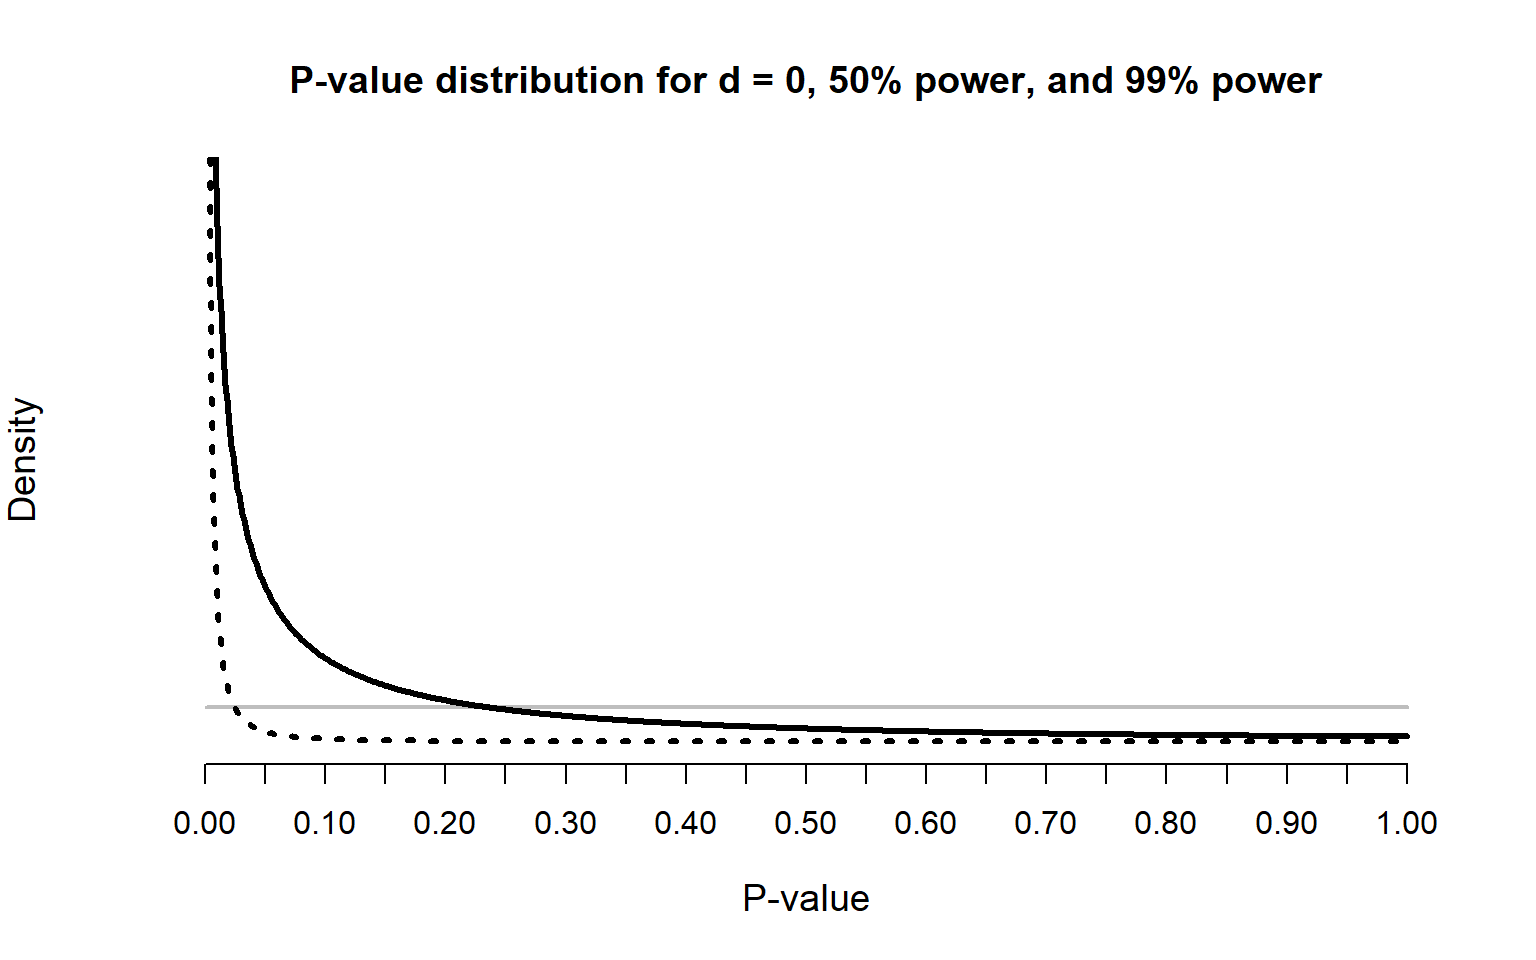
\includegraphics[width=1\linewidth]{01-pvalue_files/figure-latex/paradox-1}

\}

\textbackslash caption\{\emph{P}-value distribution for 0 (grey horizontal line, 50\% power (black solid curve), and 99\% power (black dotted curve, where \emph{p}-values just below 0.05 are more likely when H0 is true than when H1 is true).\}\label{fig:paradox}
\textbackslash end\{figure\}

\hypertarget{correctly-reporting-and-interpreting-p-values}{%
\section{\texorpdfstring{Correctly reporting and interpreting \emph{p}-values}{Correctly reporting and interpreting p-values}}\label{correctly-reporting-and-interpreting-p-values}}

Although from a strict Neyman-Pearson perspective it is sufficient to report that \emph{p} \textless{} \(\alpha\) or that \emph{p} \textgreater{} \(\alpha\), researchers should report exact \emph{p}-values. This facilitates the re-use of results for secondary analyses \citep{appelbaum_journal_2018}, and allows other researchers to compare the \emph{p}-value to an alpha level they would have preferred to use \citep{lehmann_testing_2005}. Because claims are made using a methodological procedure with known maximum error rates, a \emph{p}-value never allows you state anything with certainty. Even if we set the alpha level to 0.000001 any single claim can be an error, Fisher \citeyearpar{fisher_design_1935} reminds us, `for the ``one chance in a million'' will undoubtedly occur, with no less and no more than its appropriate frequency, however surprised we may be that it should occur to \emph{us}''. This uncertainty is sometimes not reflected in academic writing, where researchers can be seen using words as 'prove', `show', or `it is known'. A slightly longer but more accurate statement after a hypothesis test would read:

\begin{quote}
We claim there is an/no effect, while acknowledging that if scientists make claims using this methodological procedure, they will be misled, in the long run, at most alpha \% or beta \% of the time, which we deem acceptable. We will for the foreseeable future, until new data or information emerges that proves us wrong, assume this claim is correct.
\end{quote}

Remember that in a Neyman-Pearson framework researchers make claims, but do not necessarily \emph{believe} in the truth of these claims. For example, the OPERA collaboration reported in 2011 that they had observed neutrinos that traveled faster than the speed of light. This claim was made with a with a 0.2-in-a-million Type 1 error rate, \emph{assuming the error was purely due to random noise}. However, none of the researchers actually believed this claim was true, because it is theoretically impossible for neutrinos to move faster than the speed of light. Indeed, it was later confirmed that equipment failures were the cause of the anomalous data: a fiber optic cable had been attached improperly, and a clock oscillator was ticking too fast. Nevertheless, the claim was made with the explicit invitation to the scientific community to provide new data or information that would prove this claim wrong.

When researchers ``accept'' or ``reject'' a hypothesis in a Neyman-Pearson approach to statistical inferences, they do not communicate any belief or conclusion about the substantive hypothesis. Instead, they utter a Popperian \textbf{basic statement} based on a prespecified decision rule that the observed data reflect a certain state of the world. Basic statements describe an observation that has been made (e.g., ``I have observed a black swan'') or an event that has occurred (e.g., ``students performed better at the exam when being trained in spaced practice, than when not'').

The claim is about the data we have observed, but not about the theory we used to make predictions. Data never `proves' a theory is true or false. A basic statement can \textbf{corroborate} a prediction derived from a theory, or not. If many predictions deduced from a theory are corroborated, we can become increasingly convinced the theory is close to the truth. This `truth-likeness' of theories is called \textbf{verisimilitude}. A shorter statement when a hypothesis test is presented would therefore read `p = .xx, which corroborates our prediction, at an alpha level of y\%', or `p = .xx, which does not corroborate our prediction, at a statistical power of y\% for our effect size of interest'. Often, the alpha level or the statistical power is only mentioned in the experimental design section of an article, but repeating them might remind readers of the error rates associated with your claims.

Even when we have made correct claims, the underlying theory can be false. Popper (2002, p.~94) reminds us that ``The empirical basis of objective science has thus nothing `absolute' basis about it''. He argues science is not built on a solid bedrock, but on piles driven in a swamp and notes that ``We simply stop when we are satisfied that the piles are firm enough to carry the structure, at least for the time being.'' As Hacking (1965) writes: ``Rejection is not refutation. Plenty of rejections must be only tentative.'' So when we reject the null model, we do so tentatively, aware of the fact we might have done so in error, without necessarily believing the null model is false, and without believing the theory we have used to make predictions is true. For Neyman (1960, p.~13) inferential behavior is an: ``act of will to behave in the future (perhaps until new experiments are performed) in a particular manner, conforming with the outcome of the experiment''. All knowledge in science is provisional.

Some statisticians recommend interpreting \emph{p}-values as measures of \emph{evidence}. For example, Bland \citeyearpar{bland_introduction_2015} teaches that \emph{p}-values can be interpreted as a `rough and ready' guide for the strength of evidence, and that \emph{p} \textgreater{} 0.1 indicates `little or no evidence', 0.01 \textless{} \emph{p} \textless{} 0.05 indicates `evidence', \emph{p} \textless{} 0.001 is `very strong evidence'. This is incorrect \citep{lakens_why_2022}, as is clear from the previous sections on Lindley's paradox, and uniform \emph{p}-value distributions. If you want to quantify \emph{evidence}, see the chapters on {[}likelihoods{]}{[}\#likelihoods{]} or {[}Bayesian statistics{]}{[}\#bayes{]}.

\hypertarget{misconceptions}{%
\section{\texorpdfstring{Preventing common misconceptions about \emph{p}-values}{Preventing common misconceptions about p-values}}\label{misconceptions}}

A \emph{p}-value is the probability of the observed data, or more extreme data, under the assumption that the null hypothesis is true. To understand what this means, it might be especially useful to know what this doesn't mean. First, we need to know what `the assumption that the null hypothesis is true' looks like, and which data we should expect if the null hypothesis is true. Although the null hypothesis can be any value, in this assignment we will assume the null hypothesis is specified as a mean difference of 0. For example, we might be interested in calculating the difference between a control condition and an experimental condition on a dependent variable.

It is useful to distinguish the null hypothesis (the prediction that the mean difference in the population is exactly 0) and the null model (a model of the data we should expect when we collect data when the null hypothesis is true). The null hypothesis is a point at 0, but the null model is a distribution. It is visualized in textbooks or power analysis software using pictures as you can see below, with \emph{t}-values on the horizontal axis, and a critical \emph{t}-value somewhere between 1.96 -- 2.00 (depending on the sample size). This is done because the statistical test when comparing two groups is based on the \emph{t}-distribution, and the \emph{p}-value is statistically significant when the \emph{t}-value is larger than a critical \emph{t}-value.

I personally find things become a lot clearer if you plot the null model as mean differences instead of \emph{t}-values. So below, you can see a null model for the mean differences we can expect when compare two groups of 50 observations where the true difference between the two groups is 0, and the standard deviation is in each group is. Because the standard deviation is 1, you can also interpret the mean differences as a Cohen's d effect size. So this is also the distribution you can expect for a Cohen's d of 0, when collecting 50 observations per group in an independent \emph{t}-test.

\begin{figure}

{\centering 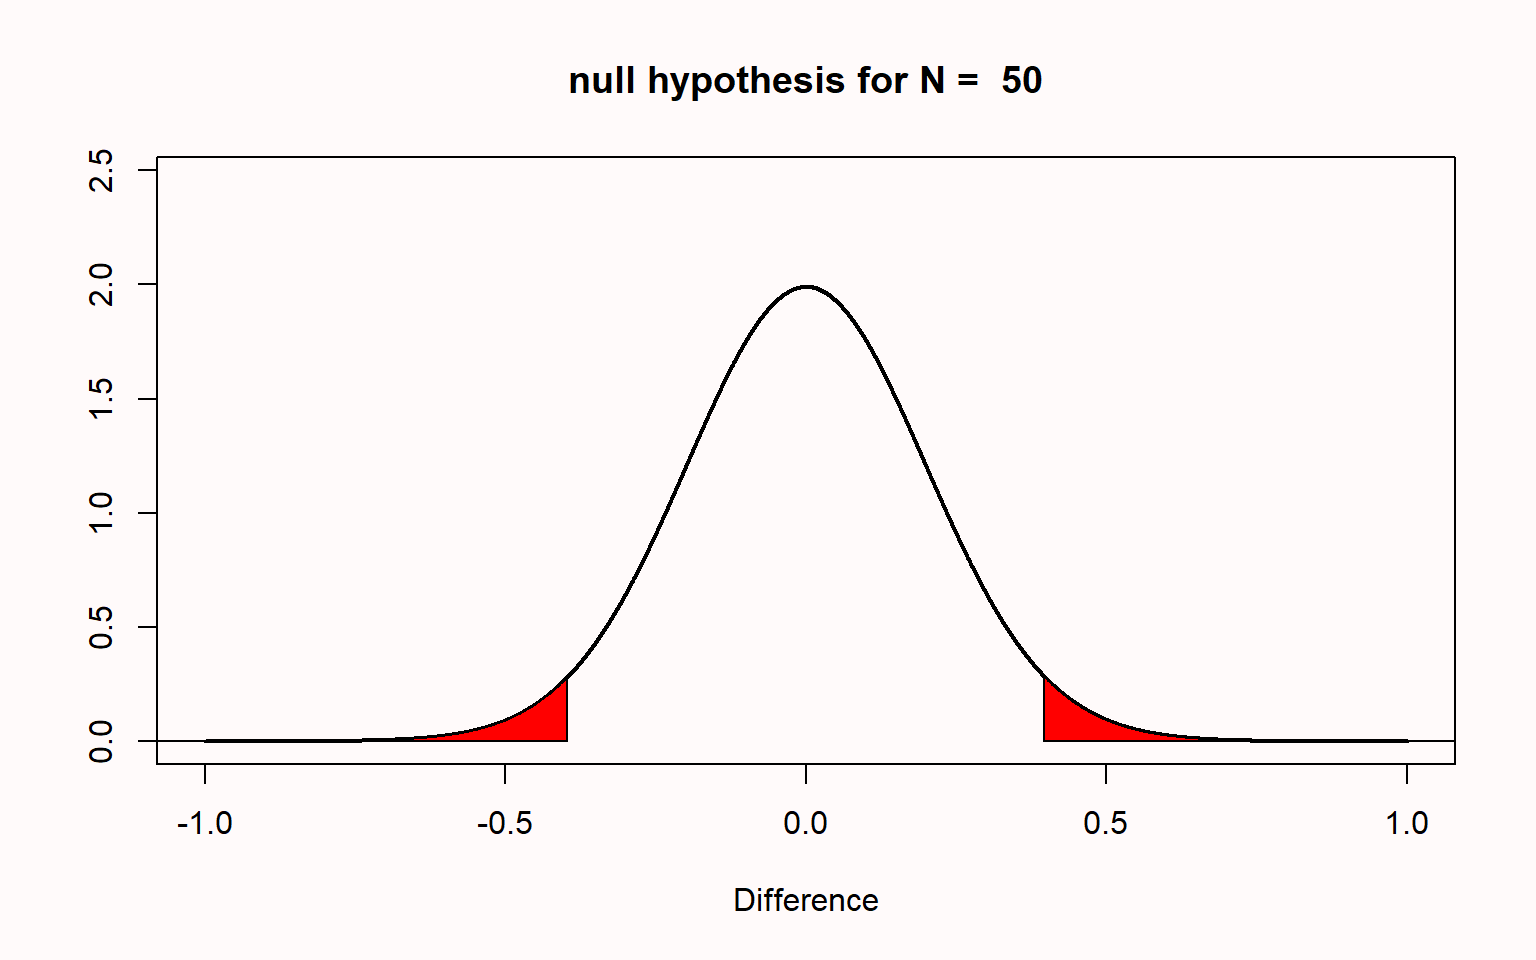
\includegraphics[width=1\linewidth]{01-pvalue_files/figure-latex/fig131-1} 

}

\caption{Distribution of observed Cohen's d effect sizes when collecting 50 observations per group in an independent t-test}\label{fig:fig131}
\end{figure}

The first thing to notice is that we expect that the mean of the null model is 0. Looking at the x-axis, we see the plotted distribution is centered on 0. But even if the mean difference in the population is 0 that does not imply every sample we draw from the population will give a mean difference of exactly zero. There is variation around the population value, as a function of the standard deviation and the sample size.

The y-axis of the graph represents the density, which provides an indication of the relative likelihood of measuring a particular value of a continuous distribution. We can see that the most likely mean difference is the true population value of zero, and that larger differences from zero become increasingly less likely. The graph has two areas that are colored red. These areas represent 2.5\% of the most extreme values in the left tail of the distribution, and 2.5\% of the most extreme values in the right tail of the distribution. Together, they make up 5\% of the most extreme mean differences we would expect to observe, given our number of observations, when the true mean difference is exactly 0. When a mean difference in the red area is observed, the corresponding statistical test will be statistically significant at a 5\% alpha level. In other words, not more than 5\% of the observed mean differences will be far enough away from 0 to be considered surprising. Because the null hypothesis is true, observing a `surprising' mean difference in the red areas is a Type 1 error.

Let's assume that the null model in the Figure above is true, and that we observe a mean difference of 0.5 between the two groups. This observed difference falls in the red area in the right tail of the distribution. This means that the observed mean difference is relatively surprising, under the assumption that the true mean difference is 0. If the true mean difference is 0, the probability density functions shows that we should not expect a mean difference of 0.5 very often. If we calculate a \emph{p}-value for this observation, it would be lower than 5\%. The probability of observing a mean difference that is at least far away from 0 as 0.5 (either to the left from the mean, or to the right, when we do a two-tailed test) is less than 5\%.

One reason why I prefer to plot the null model in raw scores instead of \emph{t}-values is that you can see how the null model changes when the sample size increases. When we collect 5000 instead of 50 observations, we see the null model is still centered on 0 -- but in our null model we now expect most values will fall very close around 0.

\begin{figure}

{\centering 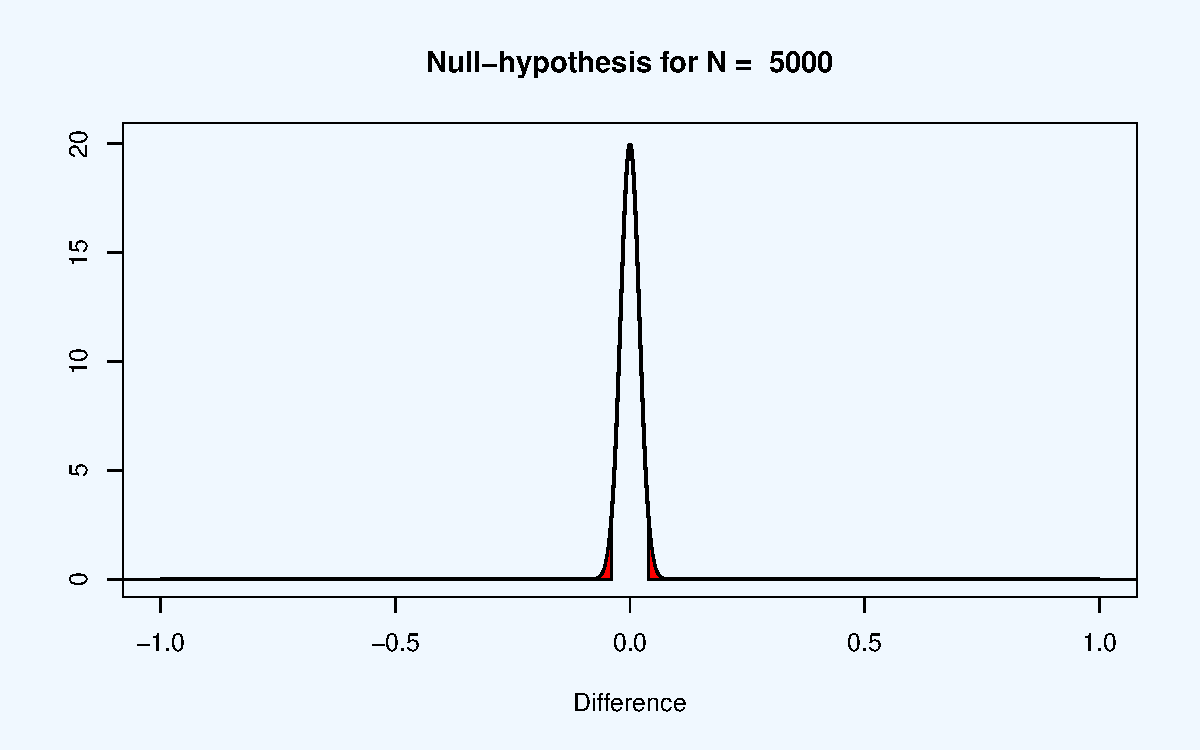
\includegraphics[width=1\linewidth]{01-pvalue_files/figure-latex/fig132-1} 

}

\caption{Distribution of observed Cohen's d effect sizes when collecting 5000 observations per group in an independent t-test when d = 0.}\label{fig:fig132}
\end{figure}

The distribution is much narrower because the distribution of mean differences is based on the standard error of the difference between means. This value is calculated based on the standard deviation and the sample size, as follows:

\[\sqrt{\frac{\sigma_{1}^{2}}{n_{1}}+\frac{\sigma_{2}^{2}}{n_{2}}}\]

This formula shows that the standard deviations of each group (σ) are squared and divided by the sample size of that group, added together, after which the square root is taken. The larger the sample size the bigger the number we divide by, and thus the smaller standard error of the difference between means. In our n = 50 example this is:

\[\sqrt{\frac{1^{2}}{50}+\frac{1^{2}}{50}}\]

The standard error of the differences between means is thus 0.2 for n = 50 in each group, and for n = 5000 it is 0.02. Assuming a normal distribution 95\% of the observations fall between 1.96 SE. So for 50 samples per group, the mean differences should fall between -1.96 * 0.2 = -0.392, and +1.96 * 0.2 = 0.392, and we can see the red areas start from approximately -0.392 to 0.392 for n = 50. For 5000 samples per group, the mean differences should fall between -1.96 * 0.02, and +1.96 * 0.02; in other words between -0.0392 to 0.0392 for n = 5000. Due to the larger sample size with n = 5000 observations per group, we should expect to observe mean differences in our sample closer to 0 compared to our null model when we had only 50 observations.

If we collected n = 5000, and we would again observe a mean difference of 0.5, it should be clear that this same difference is even more surprising than it was when we collected 50 observations. We are now almost ready to address common misconceptions about \emph{p}-values, but before we can do this, we need to introduce a model of the data when the null is not true. If we are not sampling data from a model where the true mean difference is 0, what does our alternative model look like? Some software (such as G*power, see Figure \ref{fig:gpower-screenshot}) will visualize both the null model (red curve) and the alternative model (blue curve) in their output:

\begin{figure}

{\centering 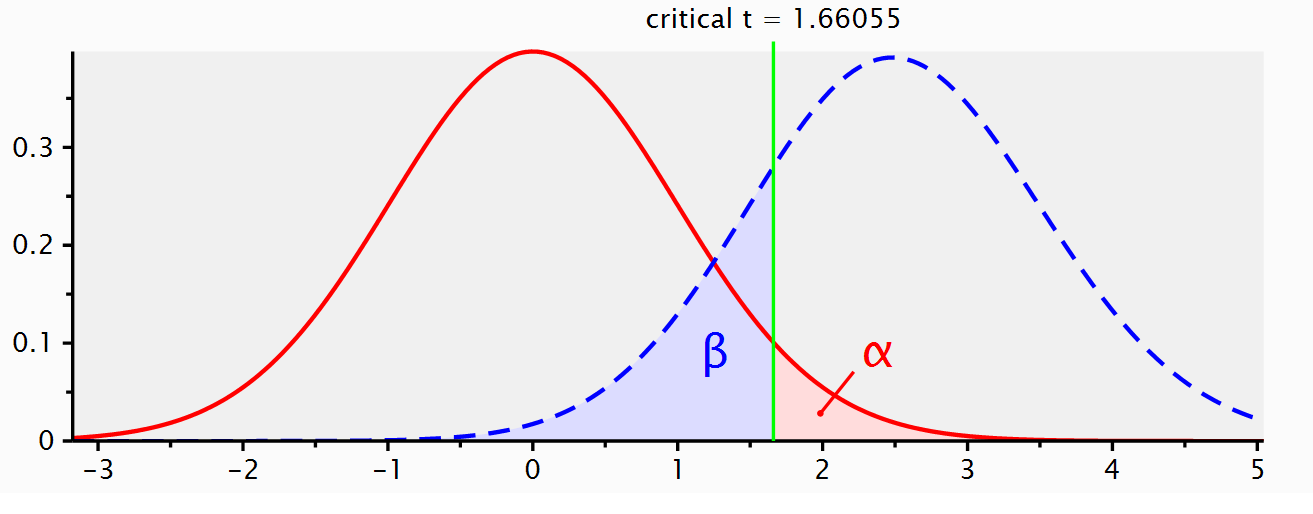
\includegraphics[width=1\linewidth]{images/1.3.3} 

}

\caption{Screenshot from Gpower software}\label{fig:gpower-screenshot}
\end{figure}

When we do a study, we rarely already know what the true mean difference is (if we already knew, why would we do the study?). But let's assume there is an all-knowing entity. Following Paul Meehl, we will call this all-knowing entity `Omniscient Jones'. Before we collect our sample of 50 observations, Omniscient Jones already knows that the true mean difference in the population is 0.5. Again, we should expect some variation around 0.5 in this alternative model. The figure below shows the expected data pattern when the null hypothesis is true (now indicated by a grey line) and it shows an alternative model, assuming a true mean difference of 0.5 exists in the population (indicated by a black line).

\begin{figure}

{\centering 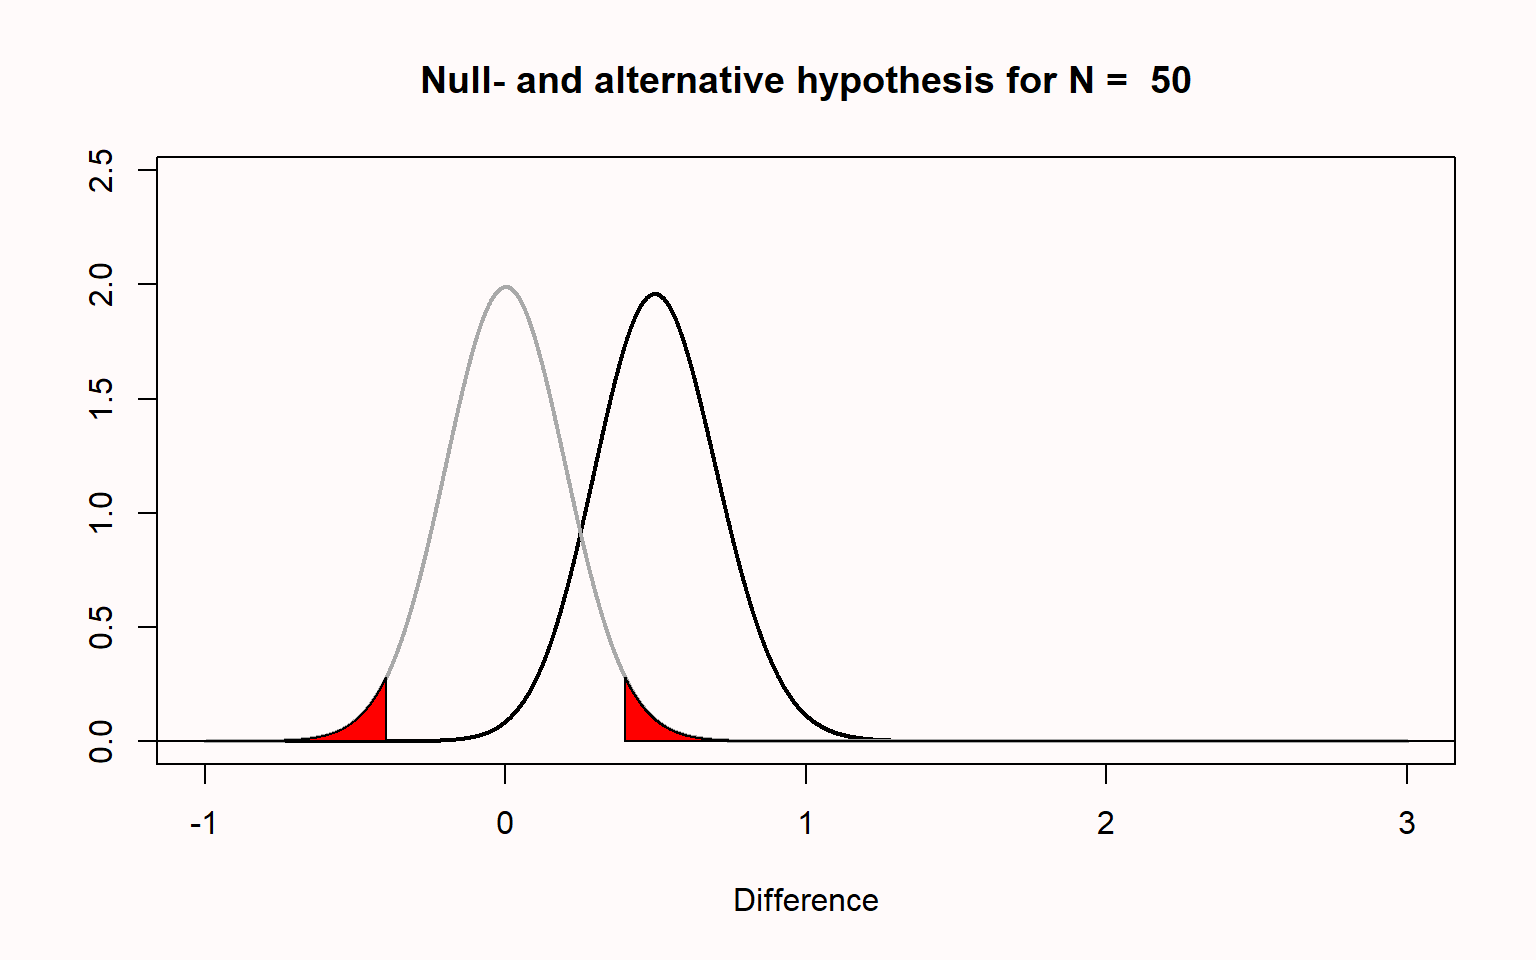
\includegraphics[width=1\linewidth]{01-pvalue_files/figure-latex/fig134-1} 

}

\caption{Distribution of observed Cohen's d effect sizes when collecting 50 observations per group in an independent t-test when d = 0.}\label{fig:fig134}
\end{figure}

But Omniscient Jones could have said the true difference was much larger. Let's assume we do another study, but now before we collect our 50 observations, Omniscient Jones tells us that the true mean difference is 1.5. The null model does not change, but the alternative model now moves over to the right.

You can play around with the alternative and null models in this online app: \url{http://shiny.ieis.tue.nl/d_p_power/}. The app allows you to specify the sample size in each group of an independent \emph{t}-test (from 2 to infinity), the mean difference (from 0 to 2), and the alpha level. In the plot, the red areas visualize Type 1 errors. The blue area visualizes the Type 2 error rate (which we will discuss below). The app also tells you the critical value: There is a vertical line (with n = 50 this line falls at a mean difference of 0.4) and a verbal label that says: ``Effects larger than 0.4 will be statistically significant''. Note that the same is true for effects smaller than -0.4, even though there is no second label there, but the app shows the situation for a two-sided independent \emph{t}-test.

You can see that on the left of the vertical line that indicates the critical mean difference there is a blue area that is part of the alternative model. This is the Type 2 error rate (or 1 - the power of the study). If a study has 80\% power, 80\% of the mean differences we will observe should fall on the right of the critical value indicated by the line. If the alternative model is true, but we observe an effect smaller than the critical value, the observed \emph{p}-value will be larger than 0.05, even when there is a true effect. You can check in the app that the larger the sample size, the further to the right the entire alternative distribution falls, and thus the higher the power. You can also see that the larger the sample size, the narrower the distribution, and the less of the distribution will fall below the critical value (as long as the true population mean is larger than the critical value). Finally, the larger the alpha level, the further to the left the critical mean difference moves, and the smaller the area of the alternative distribution that falls below the critical value.

The app also plots 3 graphs that illustrate the power curves as a function of different alpha levels, sample sizes, or true mean differences. Play around in the app by changing the values. Get a feel for how each variable impacts the null- and alternative models, the mean difference that will be statistically significant, and the Type 1 and Type 2 error rates.

So far, several aspects of null models should have become clear. First of all, the population value in a traditional null hypothesis is a value of 0, but in any sample you draw, the observed difference falls in a distribution centered on 0, and will thus most often be slightly larger or smaller than 0. Second, the width of this distribution depends on the sample size and the standard deviation. The larger the sample size in the study, the narrower the distribution will be around 0. Finally, when a mean difference is observed that falls in the tails of the null model, this can be considered surprising. The further away from the null-value, the more surprising this result is. But when the null model is true, these surprising values will happen with a probability specified by the alpha level (and are called Type 1 errors). Remember that a Type 1 error occurs when a researcher concludes there is a difference in the population, while the true mean difference in the population is zero.

We are now finally ready to address some common misconceptions about \emph{p}-values. Let's go through a list of common misconceptions that have been reported in the scientific literature. Some of these examples might sounds like semantics. It is easy to at first glance think that the statement communicates the right idea, even if the written version is not formally correct. However, when a statement is not formally correct, it is wrong. And exactly because people so often misunderstand \emph{p}-values, it is worth it to be formally correct about how they should be interpreted.

\hypertarget{misconception1}{%
\subsection{\texorpdfstring{Misunderstanding 1: A non-significant \emph{p}-value means that the null hypothesis is true}{Misunderstanding 1: A non-significant p-value means that the null hypothesis is true}}\label{misconception1}}

A common version of this misconception is reading a sentence such as `because p \textgreater{} 0.05 we can conclude that there is no effect'. Another version of such a sentence is `there was no difference, (p \textgreater{} 0.05)'.

Before we look at this misconception in some detail, I want to remind you of one fact that is easy to remember, and will enable you to recognize many misconceptions about \emph{p}-values: \emph{p}-values are a statement about the probability of data, not a statement about the probability of a hypothesis or the probability of a theory. Whenever you see \emph{p}-values interpreted as a probability of a theory or a hypothesis, you know something is not right. Examples of statements about a hypothesis are `The null hypothesis is true', or `The alternative hypothesis is true', because both these statements say that the probability that the null or alternative model is true is 100\%. A subtler version is a statement such as `the observed difference is not due to chance'. The observed difference is only `due to chance' (instead of due to the presence of a real difference) when the null hypothesis is true, and as before, this statement implies it is 100\% probable that the null hypothesis is true.

When you conclude that `there is no effect' or that `there is no difference' you are similarly claiming that it is 100\% probable that the null hypothesis is true. But since \emph{p}-values are statements about the probability of data, you should refrain from making statements about the probability of a theory solely based on a \emph{p}-value. That's ok. \emph{p}-values were designed to help you identify surprising results from a noisy data generation process (aka the real world). They were not designed to quantify the probability that a hypothesis is true.

Let's take a concrete example that will illustrate why a non-significant result does not mean that the null hypothesis is true. In the figure below, Omniscient Jones tells us the true mean difference is 0.5. We can see this, because the alternative distribution which visualized the probability of the mean differences we should expect when the null hypothesis is true is centered on 0.5. We have observed a mean difference of 0.35. This value is not extreme enough to be statistically different from 0. We can see this, because the value does not fall within the red area of the null model (and hence, the \emph{p}-value is not smaller than our alpha level).

Nevertheless, we see that observing a mean difference of 0.35 is not only quite likely given that the true mean difference is 0.5, but observing a mean difference of 0.35 is much more likely under the alternative model, than under the null model. You can see this by comparing the height of the density curve at a difference of 0.35 for the null model, which is approximately 0.5, and the height of the density curve for the alternative model, which is approximately 1.5. See the chapter on \protect\hyperlink{likettest}{likelihoods} for further details.

\begin{figure}

{\centering 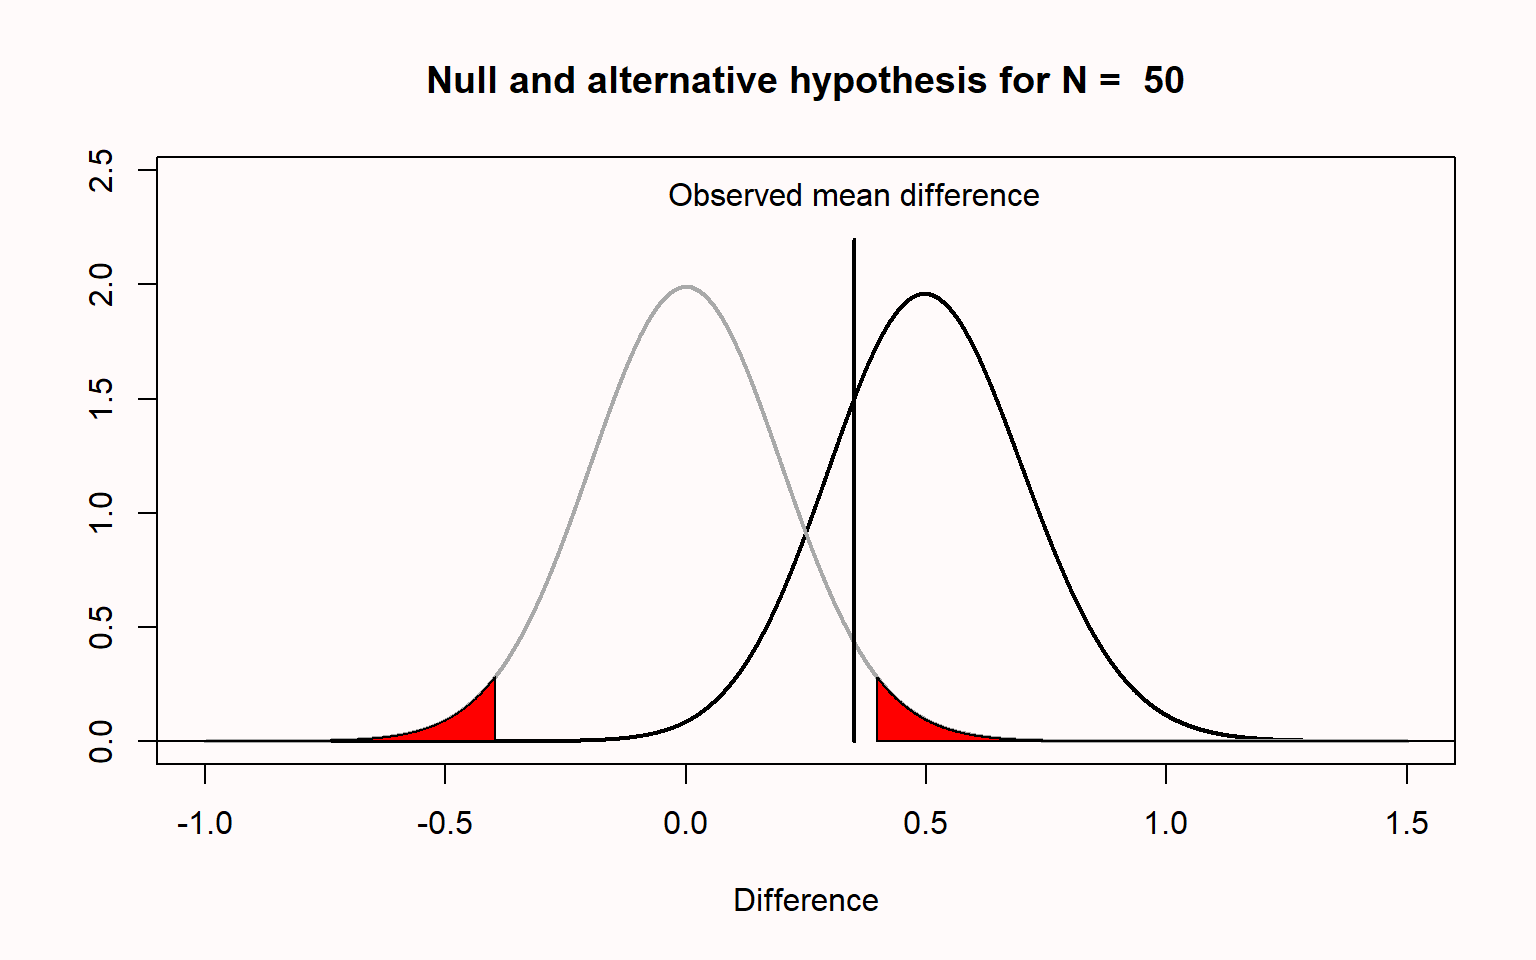
\includegraphics[width=1\linewidth]{01-pvalue_files/figure-latex/fig136-1} 

}

\caption{Distribution of observed Cohen's d effect sizes when collecting 50 observations per group in an independent t-test for d = 0 and d = 0.5 when observing d = 0.35.}\label{fig:fig136}
\end{figure}

All the \emph{p}-value tells us is that a mean difference of 0.35 is not extremely surprising, if we assume the null hypothesis is true. There can be many reasons for this. In the real world, where we have no Omniscient Jones to tell us about the true mean difference, it is possible that there is a true effect, as illustrated in the figure above.

So what should we say instead? The solution is subtle, but important. Let's revisit the two examples of incorrect statements we made earlier. First, `because p \textgreater{} 0.05 we can conclude that there is no effect' is incorrect, because there might very well be an effect (and remember \emph{p}-values are statements about data, not about the probability that there is an effect or is no effect). Fisher's interpretation of a \emph{p}-value was that we can conclude a rare event has happened, or that the null hypothesis is false (he writes literally: ``Either an exceptionally rare chance has occurred, or the theory of random distribution is not true''). This might sound like it is a statement about the probability of a theory, but it is really just stating the two possible scenarios under which low \emph{p}-values occur (when you have made a Type 1 error, or when the alternative hypothesis is true). Both remain possible, and we do not quantify the probability of either possible reality (e.g., we are not saying it is 95\% probable that the null hypothesis is false). From a Neyman-Pearson perspective a p \textgreater{} .05 means that we can not act as if the null hypothesis can be rejected, without maintaining our desired error rate of 5\%.

If you are interested in concluding an effect is absent, null hypothesis testing is not the tool to use. A null hypothesis test answers the question `can I reject the null hypothesis with a desired error rate'. If you can not do this, and p \textgreater{} 0.05, no conclusion can be drawn based only on the \emph{p}-value (remember the concept of 無 `mu': the answer is neither yes nor no). Luckily, statistical approaches have been developed to ask questions about the absence of an effect such as equivalence testing, Bayes factors, and Bayesian estimation (see Harms \& Lakens, 2018, for an overview). In the assignment in week 6 we will learn about equivalence tests in more detail.

The second incorrect statement was `there was no difference''. This statement is somewhat easier to correct. You can instead write `there was no statistically significant difference'. Granted, this is a bit tautological, because you are basically saying that the \emph{p}-value was larger than the alpha level in two different ways, but at least this statement is formally correct. The difference between `there was no difference' and `there was no statistically significant difference' might sound like semantics, but in the first case you are formally saying `the difference was 0' while in the second you are saying `there was no difference large enough to yield a \emph{p} \textless{} .05'. Although I have never seen anyone do this, a more informative message might be `because given our sample size of 50 per group, and our alpha level of 0.05, only observed differences more extreme than 0.4 could be statistically significant, and our observed mean difference was 0.35, we could not reject the null hypothesis'. If this feels like a very unsatisfactory conclusion, remember that a null hypothesis test was not designed to draw interesting conclusions about the absence of effects -- you will need to learn about equivalence tests to get a more satisfactory answers about null effects.

\hypertarget{misunderstanding-2-a-significant-p-value-means-that-the-null-hypothesis-is-false.}{%
\subsection{\texorpdfstring{Misunderstanding 2: A significant \emph{p}-value means that the null hypothesis is false.}{Misunderstanding 2: A significant p-value means that the null hypothesis is false.}}\label{misunderstanding-2-a-significant-p-value-means-that-the-null-hypothesis-is-false.}}

This is the opposite misconception from the one we discussed previously. Examples of incorrect statements based on this misconception are `\emph{p} \textless{} .05, therefore there is an effect', or `there is a difference between the two groups, \emph{p} \textless{} .05'. As before, both these statements imply it is 100\% probable that the null model is false, and an alternative model is true.

As a simple example of why such extreme statements are incorrect, imagine we generate a series of numbers in R using the following command:

\begin{Shaded}
\begin{Highlighting}[]
\FunctionTok{rnorm}\NormalTok{(}\AttributeTok{n =} \DecValTok{50}\NormalTok{, }\AttributeTok{mean =} \DecValTok{0}\NormalTok{, }\AttributeTok{sd =} \DecValTok{1}\NormalTok{)}
\end{Highlighting}
\end{Shaded}

\begin{verbatim}
##  [1]  0.93445928  0.73190335  0.15204122  2.35292028 -0.84616713 -0.24345134
##  [7]  1.62898903 -0.42592713  2.28423125 -1.12805795 -0.29486609  1.59553716
## [13]  0.12692152  1.25554797 -0.55650352  0.13851564 -0.77527366  0.93755073
## [19]  0.13614923  0.05545378 -0.91039631 -1.11189313 -2.10734020  0.23082197
## [25] -0.64751930  0.57316158  0.26222885  1.03930023 -0.24248098 -0.01789800
## [31] -0.48414605 -0.75459784 -0.40362323 -0.77782130  2.64139918 -0.90085862
## [37] -0.24909672  1.14256489  1.32081956  0.42476670 -0.99603341  1.39344806
## [43] -1.25432457 -0.04982725  1.19551213 -0.45354175 -2.61855760 -0.73605188
## [49]  0.86182370  0.71510680
\end{verbatim}

This command generates 50 random observations from a distribution with a mean of 0 and a standard deviation of 1 (in the long run -- the mean and standard deviation will vary in each sample that is generated). Imagine we run this command once, and we observe a mean of 0.5. The figure below visualizes this scenario. We can perform a one-sample \emph{t}-test against 0, and this test tells us, with a \emph{p} \textless{} .05, that the data we have observed is surprisingly different from 0, assuming the random number generator in R functions as it should and generates data with a true mean of 0.

\begin{figure}

{\centering 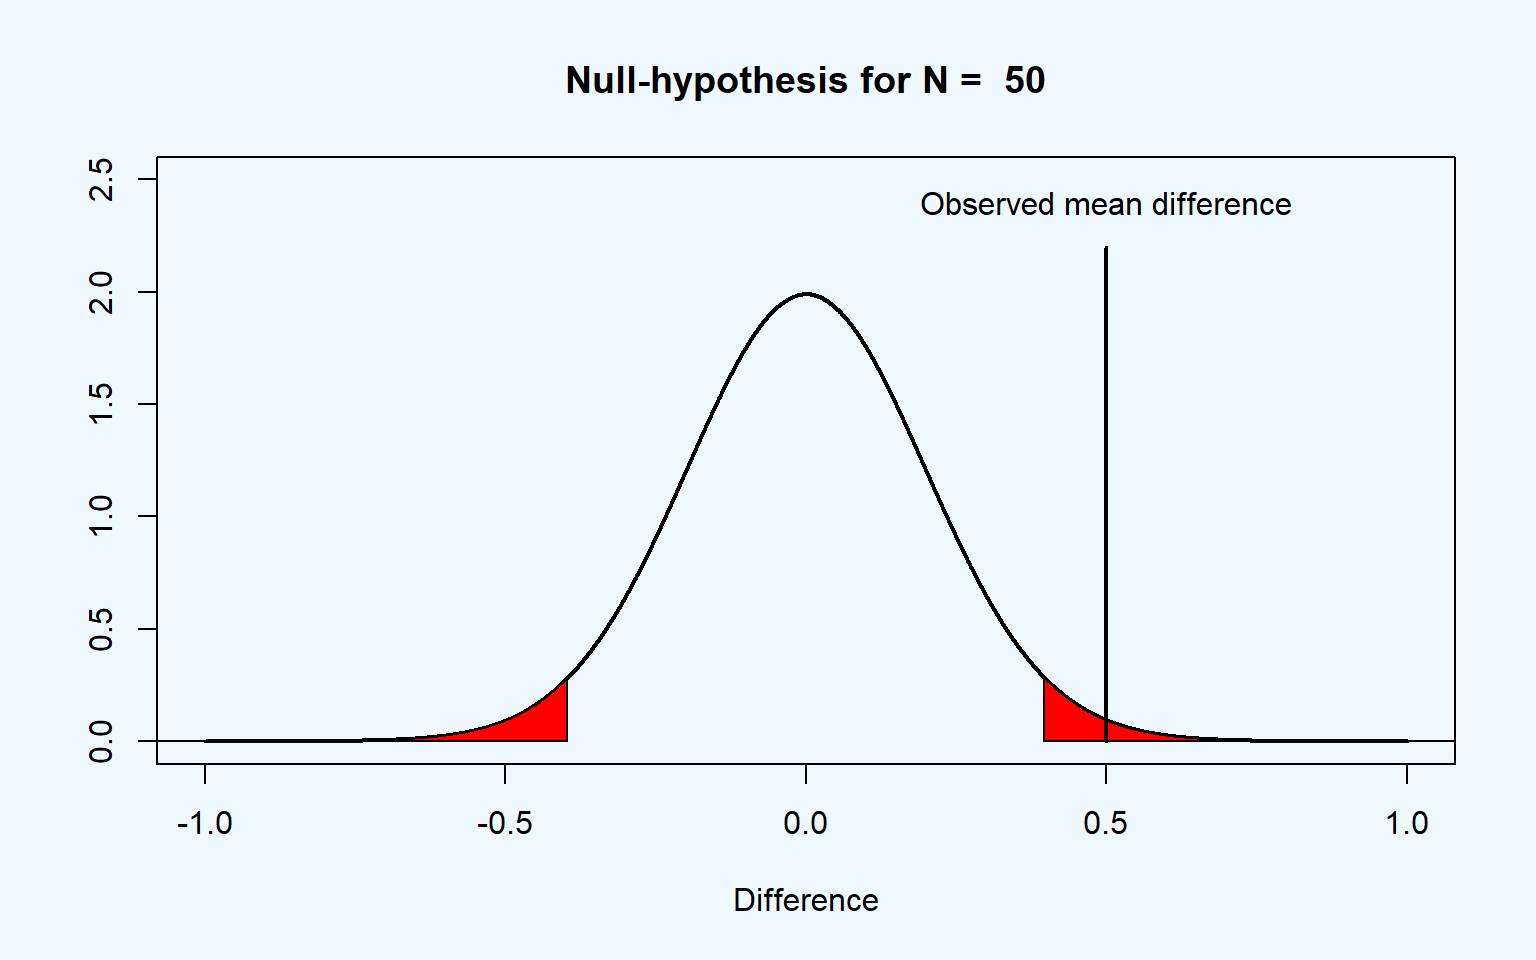
\includegraphics[width=1\linewidth]{01-pvalue_files/figure-latex/fig137-1} 

}

\caption{Distribution of observed Cohen's d effect sizes when collecting 50 observations per group in an independent t-test when d = 0 and observing d = 0.5.}\label{fig:fig137}
\end{figure}

The significant \emph{p}-value does not allow us to conclude that the null hypothesis (``the random number generator works'') is false. It is true that the mean of the 50 samples we generated was surprisingly extreme. But a low \emph{p}-value simply tells us that an observation is surprising. We should observe such surprising observations with a low probability when the null hypothesis is true -- but they still happen. Therefore, a significant result does not mean an alternative hypothesis is true -- the result can also be a Type 1 error, and in the example above, Omniscient Jones knows that this is the case.

Let's revisit the incorrect statement `\emph{p} \textless{} .05, therefore there is an effect'. A correct interpretation of a significant \emph{p}-value requires us to acknowledge the possibility that our significant result might be a Type 1 error. Remember that Fisher would conclude that ``Either an exceptionally rare chance has occurred, or the theory of random distribution is not true''. A correct interpretation in terms of Neyman Pearson statistics would be: ``we can act as if the null hypothesis is false, and we would not be wrong more than 5\% of the time in the long run''. Note the specific use of the word `act', which does not imply anything about whether this specific hypothesis is true or false, but merely states that if we act as if the null-hypothesis is false any time we observe \emph{p} \textless{} alpha, we will not make an error more than alpha percent of the time.

Both these formally correct statements are a bit long. In scientific articles, we often read a shorter statement such as: `we can reject the null hypothesis', or `we can accept the alternative hypothesis'. These statements might be made with the assumption that readers will themselves add `with a 5\% probability of being wrong, in the long run'. But it might be useful to add `with a 5\% long run error rate' at least the first time you make such a statement in your article to remind readers.

In the example above we have a very strong subjective prior probability that the random number generator in R works. Alternative statistical procedures to incorporate such prior beliefs are Bayesian statistics (week 2) or false positive report probabilities (week 3). In frequentist statistics, the idea is that you need to replicate your study several times. You will observe a Type 1 error every now and then, but you are unlikely to observe a Type 1 error three times in a row. Alternatively, you can lower the alpha level in a single study to reduce the probability of a Type 1 error rate.

\hypertarget{misunderstanding-3-a-significant-p-value-means-that-a-practically-important-effect-has-been-discovered}{%
\subsection{\texorpdfstring{Misunderstanding 3: A significant \emph{p}-value means that a practically important effect has been discovered}{Misunderstanding 3: A significant p-value means that a practically important effect has been discovered}}\label{misunderstanding-3-a-significant-p-value-means-that-a-practically-important-effect-has-been-discovered}}

A common concern when interpreting \emph{p}-values is that `significant' in normal language implies `important', and thus a `significant' effect is interpreted as an `important' effect. However, the question whether an effect is important is completely orthogonal to the question whether it is different from zero, or even how large the effect is. Not all effects have practical impact. The smaller the effect, the less likely such effects will be noticed by individuals, but such effects might still have a large impact on a societal level. Therefore, the general take home message is that statistical significance does not answer the question whether an effect matters in practice, or is `practically important'. To answer the question whether an effect matters, you need to present a cost-benefit analysis.

This issue of practical significance most often comes up in studies with a very large sample size. As we have seen before, with an increasing sample size, the width of the density distribution around the null-value becomes more and more narrow, and the values that are considered surprising fall closer and closer to zero.

If we plot the null model for a very large sample size (e.g., n = 10000 per group) we see that even very small mean differences (differences more extreme than a mean difference of 0.04) will be considered `surprising'. This still means that if there really is no difference in the population, you will observe differences larger than 0.04 less than 5\% of the time, in the long run, and 95\% of the observed differences will be smaller than a mean difference of 0.04. But it becomes more difficult to argue for the practical significance of such effects. Imagine that a specific intervention is successful in changing people's spending behavior, and when implementing some intervention people save 12 cents per year. It is difficult to argue how this effect will make any individual happier. However, if this money is combined, it will yield over 2 million, which could be used to treat diseases in developing countries, where it would have a real impact. The cost of the intervention might be considered too high if the goal is to make individuals happier, but it might be consider worthwhile if the goal is to raise 2 million for charity.

Not all effects in psychology are additive (we can not combine or transfer an increase in happiness of 0.04 scale points), so it is often more difficult to argue for the importance of small effects in subjective feelings. A cost-benefit analysis might show small effects matter a lot, but whether or not this is the case can not be inferred from a \emph{p}-value.

Note that nothing about this is a problem with the interpretation of a \emph{p}-value per se: A \emph{p} \textless{} 0.05 still correctly indicates that, if the null hypothesis is true, we have observed data that should be considered surprising. However, just because data is surprising, does not mean we need to care about it. It is mainly the verbal label `significant' that causes confusion here -- it is perhaps less confusing to think of a `significant' effect as a `surprising' effect, but not necessarily as an `important' effect.

\hypertarget{misconception4}{%
\subsection{Misunderstanding 4: If you have observed a significant finding, the probability that you have made a Type 1 error (a false positive) is 5\%.}\label{misconception4}}

This misinterpretation is one possible explanation of the incorrect statement that a \emph{p}-value is `the probability that the data are observed by chance.' Assume we collect 20 observations, and Omniscient Jones tells us the null hypothesis is true (as in the example above where we generated random numbers in R). This means we are sampling from the distribution in the figure below.

\begin{figure}

{\centering 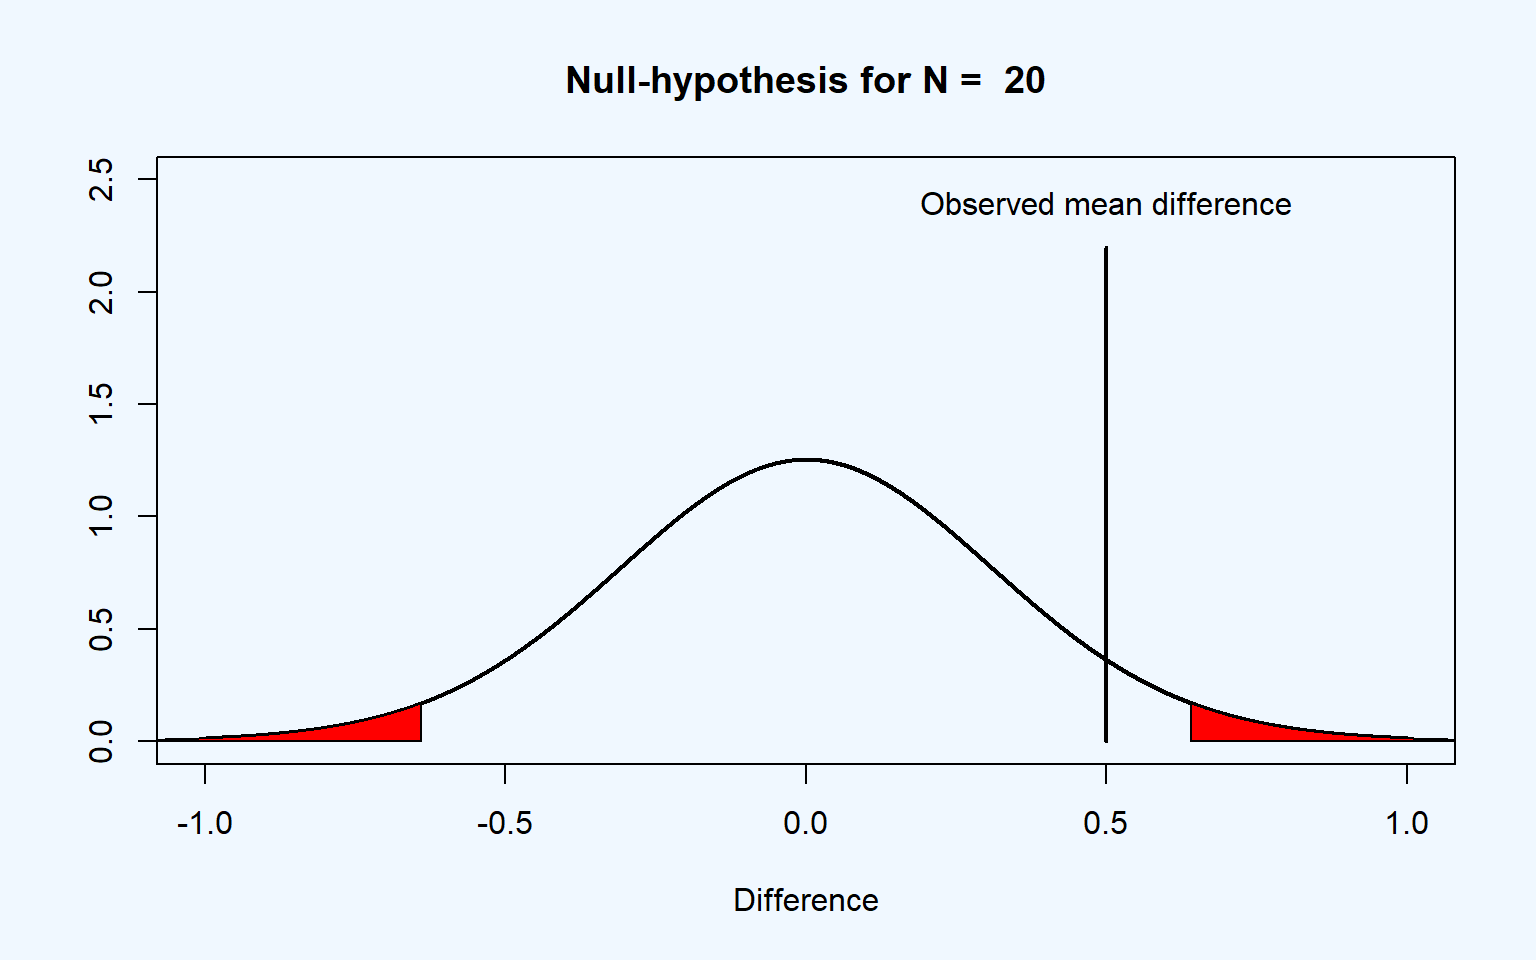
\includegraphics[width=1\linewidth]{01-pvalue_files/figure-latex/fig138-1} 

}

\caption{Distribution of observed Cohen's d effect sizes when collecting 20 observations per group in an independent t-test when d = 0.}\label{fig:fig138}
\end{figure}

If this is our reality, it means that 100\% of the time that we observe a significant result, it is a false positive (or Type I error). Thus, 100\% of our significant results are Type 1 errors.

It is important to distinguish probabilities before collecting the data and analyzing the result, and probabilities after collecting data and analyzing the results. What the Type 1 error rate controls, is that from all studies we will perform in the future where the null hypothesis is true, not more than 5\% of our observed mean differences will fall in the red tail areas. But after we have seen that our data falls in the tail areas with \emph{p} \textless{} alpha, and we know that the null hypothesis is true, these observed significant effects are always a Type 1 error. If you read carefully, you will notice that this misunderstanding is cause by differences in the question that is asked. ``If I have observed a \emph{p} \textless{} .05, what is the probability that the null hypothesis is true?'' is a different question than ``If the null hypothesis is true, what is the probability of observing this (or more extreme) data''. Only the latter question is answered by a \emph{p}-value. The first question can not be answered without making a subjective judgment about the probability that the null hypothesis is true prior to collecting the data (see the lectures on Bayesian statistics in week 2).

\hypertarget{misunderstanding-5-one-minus-the-p-value-is-the-probability-that-the-effect-will-replicate-when-repeated.}{%
\subsection{\texorpdfstring{Misunderstanding 5: One minus the \emph{p}-value is the probability that the effect will replicate when repeated.}{Misunderstanding 5: One minus the p-value is the probability that the effect will replicate when repeated.}}\label{misunderstanding-5-one-minus-the-p-value-is-the-probability-that-the-effect-will-replicate-when-repeated.}}

It is impossible to calculate the probability that an effect will replicate, based on only the \emph{p}-value. The main reason for this is that we do not know the true mean difference. If we were Omniscient Jones, and we knew the true mean difference (e.g., a difference between the two groups of 0.5 scale points) we would know the statistical power of our test. The statistical power is the probability that we will find a significant result, if the alternative model is true (i.e.~if there is a true effect). For example, reading the text in the left bar in the app, we see that with N = 50 per group, and alpha level of 0.05, and a true mean difference of 0.5, the probability of finding a significant result (or the statistical power) is 69.69\%. If we would observe a significant effect in this scenario (e.g., \emph{p} = 0.03) it is not true that there is a 97\% probability that an exact replication of the study (with the same sample size) would again yield a significant effect. The probability that a study yields a significant effect is determined by the statistical power - not by the \emph{p}-value in a previous study.
What we can generally take away from this last misunderstanding is the fact that the probability of replication depends on the presence versus the absence of a true effect. In other words, as stated above, if a true effect exists then the level of statistical power informs us about how frequently we should yield a significant result (e.g., 80\% power means we should observe significant result 80\% of the time). On the other hand, if the effect is null (or non-existent) then significant results will be observed only 5\% of the time in the long run (i.e.~the Type 1 error rate given an alpha of 0.05). Therefore, either the statistical power or the alpha level equals the probability of replication, depending on if there is or isn't a true effect.

\hypertarget{test-yourself}{%
\section{Test Yourself}\label{test-yourself}}

\hypertarget{questions-about-which-p-values-you-can-expect}{%
\subsection{\texorpdfstring{Questions about which \emph{p}-values you can expect}{Questions about which p-values you can expect}}\label{questions-about-which-p-values-you-can-expect}}

Copy the code below to R and run the code.

\begin{Shaded}
\begin{Highlighting}[]
\NormalTok{nsims }\OtherTok{\textless{}{-}} \DecValTok{100000} \CommentTok{\# number of simulations}

\NormalTok{m }\OtherTok{\textless{}{-}} \DecValTok{106} \CommentTok{\# mean sample}
\NormalTok{n }\OtherTok{\textless{}{-}} \DecValTok{26} \CommentTok{\# set sample size}
\NormalTok{sd }\OtherTok{\textless{}{-}} \DecValTok{15} \CommentTok{\# SD of the simulated data}

\NormalTok{p }\OtherTok{\textless{}{-}} \FunctionTok{numeric}\NormalTok{(nsims) }\CommentTok{\# set up empty vector}
\NormalTok{bars }\OtherTok{\textless{}{-}} \DecValTok{20}

\ControlFlowTok{for}\NormalTok{ (i }\ControlFlowTok{in} \DecValTok{1}\SpecialCharTok{:}\NormalTok{nsims) \{ }\CommentTok{\# for each simulated experiment}
\NormalTok{  x }\OtherTok{\textless{}{-}} \FunctionTok{rnorm}\NormalTok{(}\AttributeTok{n =}\NormalTok{ n, }\AttributeTok{mean =}\NormalTok{ m, }\AttributeTok{sd =}\NormalTok{ sd)}
\NormalTok{  z }\OtherTok{\textless{}{-}} \FunctionTok{t.test}\NormalTok{(x, }\AttributeTok{mu =} \DecValTok{100}\NormalTok{) }\CommentTok{\# perform the t{-}test}
\NormalTok{  p[i] }\OtherTok{\textless{}{-}}\NormalTok{ z}\SpecialCharTok{$}\NormalTok{p.value }\CommentTok{\# get the p{-}value}
\NormalTok{\}}
\NormalTok{power }\OtherTok{\textless{}{-}} \FunctionTok{round}\NormalTok{((}\FunctionTok{sum}\NormalTok{(p }\SpecialCharTok{\textless{}} \FloatTok{0.05}\NormalTok{) }\SpecialCharTok{/}\NormalTok{ nsims), }\DecValTok{2}\NormalTok{) }\CommentTok{\# power}

\CommentTok{\# Plot figure}
\FunctionTok{hist}\NormalTok{(p,}
  \AttributeTok{breaks =}\NormalTok{ bars, }\AttributeTok{xlab =} \StringTok{"P{-}values"}\NormalTok{, }\AttributeTok{ylab =} \StringTok{"number of p{-}values}\SpecialCharTok{\textbackslash{}n}\StringTok{"}\NormalTok{, }
  \AttributeTok{axes =} \ConstantTok{FALSE}\NormalTok{,  }\AttributeTok{main =} \FunctionTok{paste}\NormalTok{(}\StringTok{"P{-}value Distribution with"}\NormalTok{, }
                              \FunctionTok{round}\NormalTok{(power }\SpecialCharTok{*} \DecValTok{100}\NormalTok{, }\AttributeTok{digits =} \DecValTok{1}\NormalTok{), }\StringTok{"\% Power"}\NormalTok{),}
  \AttributeTok{col =} \StringTok{"grey"}\NormalTok{, }\AttributeTok{xlim =} \FunctionTok{c}\NormalTok{(}\DecValTok{0}\NormalTok{, }\DecValTok{1}\NormalTok{), }\AttributeTok{ylim =} \FunctionTok{c}\NormalTok{(}\DecValTok{0}\NormalTok{, nsims))}
\FunctionTok{axis}\NormalTok{(}\AttributeTok{side =} \DecValTok{1}\NormalTok{, }\AttributeTok{at =} \FunctionTok{seq}\NormalTok{(}\DecValTok{0}\NormalTok{, }\DecValTok{1}\NormalTok{, }\FloatTok{0.1}\NormalTok{), }\AttributeTok{labels =} \FunctionTok{seq}\NormalTok{(}\DecValTok{0}\NormalTok{, }\DecValTok{1}\NormalTok{, }\FloatTok{0.1}\NormalTok{))}
\FunctionTok{axis}\NormalTok{(}\AttributeTok{side =} \DecValTok{2}\NormalTok{, }\AttributeTok{at =} \FunctionTok{seq}\NormalTok{(}\DecValTok{0}\NormalTok{, nsims, nsims }\SpecialCharTok{/} \DecValTok{4}\NormalTok{), }
     \AttributeTok{labels =} \FunctionTok{seq}\NormalTok{(}\DecValTok{0}\NormalTok{, nsims, nsims }\SpecialCharTok{/} \DecValTok{4}\NormalTok{), }\AttributeTok{las =} \DecValTok{2}\NormalTok{)}
\FunctionTok{abline}\NormalTok{(}\AttributeTok{h =}\NormalTok{ nsims }\SpecialCharTok{/}\NormalTok{ bars, }\AttributeTok{col =} \StringTok{"red"}\NormalTok{, }\AttributeTok{lty =} \DecValTok{3}\NormalTok{)}
\end{Highlighting}
\end{Shaded}

\begin{center}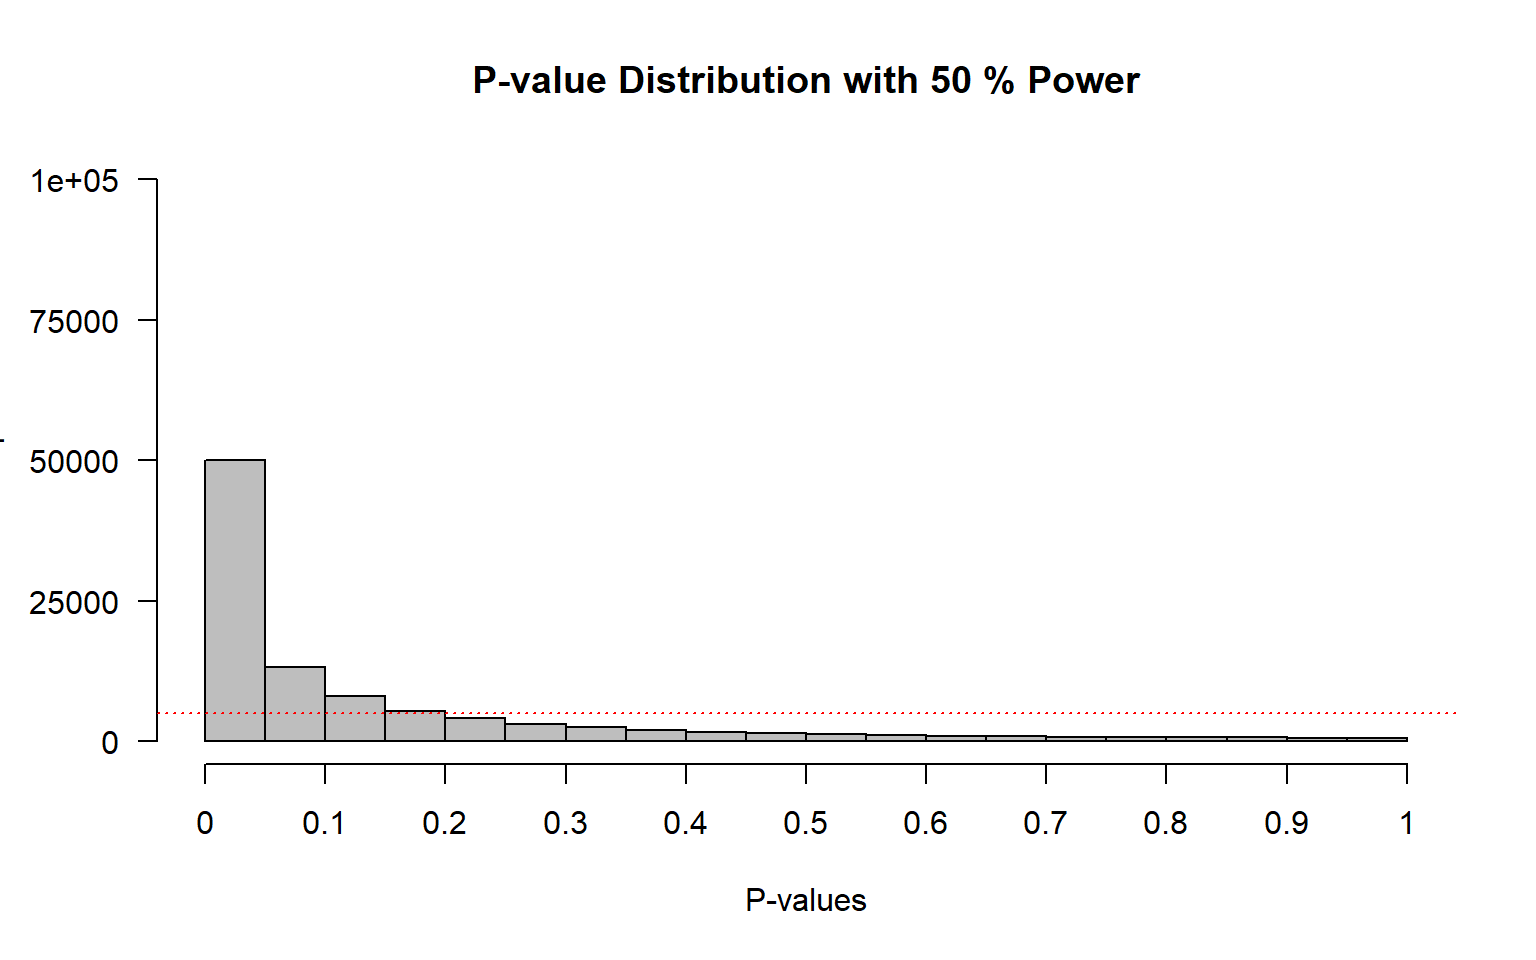
\includegraphics[width=1\linewidth]{01-pvalue_files/figure-latex/q1-1} \end{center}

On the x-axis we see \emph{p}-values from 0 to 1 in 20 bars, and on the y-axis we see how frequently these \emph{p}-values were observed. There is a horizontal red dotted line that indicates an alpha of 5\% (located at a frequency of 100.000*0.05 = 5000) -- but you can ignore this line for now. In the title of the graph, the statistical power that is achieved in the simulated studies is given (assuming an alpha of 0.05): The studies have 50\% power (with minor variations for each simulation).

\textbf{Q1}: Since the statistical power is the probability of observing a statistically significant result, if there is a true effect, we can also see the power in the figure itself. Where?

\begin{enumerate}
\def\labelenumi{\Alph{enumi})}
\tightlist
\item
  We can calculate the number of \emph{p}-values larger than 0.5, and divide them by the number of simulations.
\item
  We can calculate the number of \emph{p}-values in the first bar (which contains all `significant' \emph{p}-values from 0.00 to 0.05) and divide the \emph{p}-values in this bar by the total number of simulations.
\item
  We can calculate the difference between \emph{p}-values above 0.5 minus the \emph{p}-values below 0.5, and divide this number by the total number of simulations.
\item
  We can calculate the difference between \emph{p}-values above 0.5 minus the \emph{p}-values below 0.05, and divide this number by the number of simulations.
\end{enumerate}

\textbf{Q2}: Change the sample size from n \textless- 26 to n \textless- 51. Run the simulation by selecting all lines and pressing CTRL+Enter. What is the power in the simulation now that we have increased the sample size from 26 people to 51 people?

\begin{enumerate}
\def\labelenumi{\Alph{enumi})}
\tightlist
\item
  55\%
\item
  60\%
\item
  80\%
\item
  95\%
\end{enumerate}

\textbf{Q3}: If you look at the distribution of \emph{p}-values, what do you notice?

\begin{enumerate}
\def\labelenumi{\Alph{enumi})}
\tightlist
\item
  The \emph{p}-value distribution is exactly the same as with 50\% power
\item
  The \emph{p}-value distribution is much steeper than with 50\% power
\item
  The \emph{p}-value distribution is much flatter than with 50\% power
\item
  The \emph{p}-value distribution is much more normally distributed than with 50\% power
\end{enumerate}

Feel free to increase and decrease the sample size and see what happens if you run the simulation. When you are done exploring, make sure that n \textless- 51 again.

\textbf{Q4}: What would happen when there is no true difference between our simulated samples and the average IQ score? In this situation, we have no probability to observe an effect, so you might say we have `0 power'. Formally, power is not defined when there is no true effect. However, we can casually refer to this as 0 power. Change the mean in the sample to 100 (set m \textless- 106 to m \textless- 100) There is now no difference between the mean in our sample, and the population value we are testing against in the one-sample \emph{t}-test. Run the script again. What do you notice?

\begin{enumerate}
\def\labelenumi{\Alph{enumi})}
\tightlist
\item
  The \emph{p}-value distribution is exactly the same as with 50\% power
\item
  The \emph{p}-value distribution is much steeper than with 50\% power
\item
  The \emph{p}-value distribution is basically completely flat (ignoring some minor variation due to random noise in the simulation)
\item
  The \emph{p}-value distribution is normally distributed
\end{enumerate}

The question below builds on the simulation above where there was no true difference between the groups.

\textbf{Q5}: Look at the leftmost bar in the plot produced for Q4, and look at the frequency of \emph{p}-values in this bar What is the formal name for this bar?

\begin{enumerate}
\def\labelenumi{\Alph{enumi})}
\tightlist
\item
  The power (or true positives)
\item
  The true negatives
\item
  The Type 1 error (or false positives)
\item
  The Type 2 error (or false negatives)
\end{enumerate}

Let's take a look at just the \emph{p}-values below 0.05. Bear with me for the next few steps -- it will be worth it. Find the variable that determines how many bars there are, in the statement bars \textless- 20. Change it to bars \textless- 100. We will now get 1 bar for \emph{p}-values between 0 and 0.01, one bar for \emph{p}-values between 0.01 and 0.02, and 100 bars in total. The red dotted line will now indicate the frequency of \emph{p}-values when the null hypothesis is true, where every bar contains 1\% of the total number of \emph{p}-values. We only want to look at \emph{p}-values below 0.05, and we will cut off the plot at 0.05. Change xlim = c(0, 1) to xlim = c(0, 0.05). Instead of seeing all \emph{p}-values between 0 and 1, we will only see \emph{p}-values between 0 and 0.05. Re-run the simulation (still with m \textless- 100). We see the same uniform distribution, but now every bar contains 1\% of the \emph{p}-values, so the \emph{p}-value distribution is very flat and almost impossible to see (we will zoom in on the y-axis later this assignment). The red line now clearly gives the frequency for each bar, assuming the null hypothesis is true.

Change the mean in the simulation in line 9 to m \textless- 107 (remember n is still 51). Re-run the simulation. It's clear we have very high power. Most \emph{p}-values are in the left-most bar, which contains all \emph{p}-values between 0.00 and 0.01.

\textbf{Q6}: The plot from the last simulation tells you we have 90.5\% power. This is the power if we use an alpha of 5\%. But we can also use an alpha of 1\%. What is the statistical power we have in the simulated studies when we would use an alpha of 1\%, looking at the graph? Pick the answer closest to the answer from your simulations.

\begin{enumerate}
\def\labelenumi{\Alph{enumi})}
\tightlist
\item
  \textasciitilde90\%
\item
  \textasciitilde75\%
\item
  \textasciitilde50\%
\item
  \textasciitilde5\%
\end{enumerate}

To be able to look at the \emph{p}-values around 0.03 and 0.04, we will zoom in on the y-axis as well. In the part of the code where the plot is draw, change ylim = c(0, nSims) to ylim = c(0, 10000). Re-run the script.

Change the mean in the sample to 108 in m \textless- 108), and leave the sample size at 51. Run the simulation. Look at how the distribution has changed compared to the graph above.

Look at the fifth bar from the left. This bar now contains all the \emph{p}-values between 0.04 and 0.05. You will notice something peculiar. Remember that the red dotted line indicates the frequency in each bar, assuming the null hypothesis is true. See how the bar with \emph{p}-values between 0.04 and 0.05 is lower than the red line. We have simulated studies with 96\% power. When power is very high, \emph{p}-values between 0.04 and 0.05 are very rare -- they occur less than 1\% of the time (most \emph{p}-values are smaller than 0.01). When the null hypothesis is true, \emph{p}-values between 0.04 and 0.05 occur exactly 1\% of the time (because \emph{p}-values are uniformly distributed). Now ask yourself: When you have very high power, and you observe a \emph{p}-value between 0.04 and 0.05, is it more likely that the null-hypothesis is true, or that the alternative hypothesis is true? Given that you are more likely to observe \emph{p}-values between 0.04 and 0.05 when the null hypothesis is true, than when the alternative hypothesis is true, you should interpret a \emph{p}-value significant with an alpha of 0.05 as more likely when the null hypothesis is true, than when the alternative hypothesis is true.

In our simulations, we know there is a true effect or not, but in the real world, you don't know. When you have very high power, use an alpha level of 0.05, and find a \emph{p}-value of \emph{p} = .045, the data is surprising, assuming the null hypothesis is true, but it is even \emph{more} surprising, assuming the alternative hypothesis is true. This shows how a significant \emph{p}-value is not always evidence for the alternative hypothesis.

\textbf{Q7}: When you know you have very high (e.g., 98\%) power for the smallest effect size you care about, and you observe a \emph{p}-value of 0.045, what is the correct conclusion?

\begin{enumerate}
\def\labelenumi{\Alph{enumi})}
\tightlist
\item
  The effect is significant, and provides strong support for the alternative hypothesis.
\item
  The effect is significant, but it is without any doubt a Type 1 error.
\item
  With high power, you should use an alpha level that is smaller than 0.05, and therefore, this effect can not be considered significant.
\item
  The effect is significant, but the data are more likely under the null hypothesis than under the alternative hypothesis.
\end{enumerate}

\textbf{Q8}: Play around with the sample size (n) and the mean (m) by changing the numerical values or both (and thus, vary the statistical power in the simulated studies). Look at the simulation result for the bar that contains \emph{p}-values between 0.04 and 0.05. The red line indicates how many \emph{p}-values would be found in this bar if the null-hypothesis was true (and is always at 1\%). At the very best, how much more likely is a \emph{p}-value between 0.04 and 0.05 to come from a \emph{p}-value distribution representing a true effect, than it is to come from a \emph{p}-value distribution when there is no effect? You can answer this question by seeing how much higher the bar of \emph{p}-values between 0.04 and 0.05 can become. If at best the bar in the simulation is five times as high at the red line (so the bar shows 5\% of \emph{p}-values end up between 0.04 and 0.05, while the red line remains at 1\%), then at best \emph{p}-values between 0.04 and 0.05 are five times as likely when there is a true effect than when there is no true effect.

\begin{enumerate}
\def\labelenumi{\Alph{enumi})}
\tightlist
\item
  At best, \emph{p}-values between 0.04 and 0.05 are equally likely under the
  alternative hypothesis, and under the null hypothesis.
\item
  At best, \emph{p}-values between 0.04 and 0.05 are approximately 4 times more
  likely under the alternative hypothesis, than under the null hypothesis.
\item
  At best, \emph{p}-values between 0.04 and 0.05 are \textasciitilde10 times more likely under the alternative hypothesis, than under the null hypothesis.
\item
  At best, \emph{p}-values between 0.04 and 0.05 are \textasciitilde30 times more likely under the alternative hypothesis, than under the null hypothesis.
\end{enumerate}

For this reason, statisticians warn that \emph{p}-values just below 0.05 (e.g.,
between 0.04 and 0.05) are at the very best weak support for the alternative
hypothesis. If you find \emph{p}-values in this range, consider replicating the
study, or if that's not possible, interpret the result at least a bit
cautiously.

\hypertarget{questions-about-p-value-misconceptions}{%
\subsection{\texorpdfstring{Questions about \emph{p}-value misconceptions}{Questions about p-value misconceptions}}\label{questions-about-p-value-misconceptions}}

\textbf{Q1}: When the sample size in each group of an independent \emph{t}-test is 50
observations (see Figure \ref{fig:fig131}), which statement is correct?

\begin{enumerate}
\def\labelenumi{\Alph{enumi})}
\tightlist
\item
  The mean of the differences you will observe between the two groups is always 0.
\item
  The mean of the differences you will observe between the two groups is always different from 0.
\item
  Observing a mean difference of +0.5 or -0.5 is considered surprising, assuming the null hypothesis is true.
\item
  Observing a mean difference of +0.1 or -0.1 is considered surprising, assuming the null hypothesis is true.
\end{enumerate}

\textbf{Q2:} In what sense are the null models in the figures (Figure \ref{fig:fig131} and \ref{fig:fig132}) similar, and in what sense are they different?

\begin{enumerate}
\def\labelenumi{\Alph{enumi})}
\tightlist
\item
  In both cases, the distributions are centered on zero, and the critical
  \emph{t}-value is between 1.96 and 2 (for a two-sided test, depending on the sample size). But the larger the sample size, the closer to 0 the mean differences fall that are considered `surprising'.
\item
  In both cases, a \emph{t}-value of 0 is the most likely outcome, but the critical \emph{t}-value is around 0.4 for n = 50, and around 0.05 for n = 5000.
\item
  In both cases, means will vary in exactly the same way around 0, but the Type 1 error rate is much smaller when n = 5000 than when n = 50.
\item
  Because the standard error is much larger for n = 50 than for n = 5000, it is much more likely that the null hypothesis is true for n = 50.
\end{enumerate}

\textbf{Q3:} You can play around with the alternative and null models in this online app: \url{http://shiny.ieis.tue.nl/d_p_power/}. The app allows you to specify the sample size in each group of an independent \emph{t}-test (from 2 to infinity), the mean difference (from 0 to 2), and the alpha level. In the plot, the red areas visualize Type 1 errors. The blue area visualizes the Type 2 error rate (which we will discuss below). The app also tells you the critical value: There is a vertical line (with n = 50 this line falls at a mean difference of 0.4) and a verbal label that says: ``Effects larger than 0.4 will be statistically significant''. Note that the same is true for effects smaller than -0.4, even though there is no second label there, but the app shows the situation for a two-sided independent \emph{t}-test.

You can see that on the left of the vertical line that indicates the critical mean difference there is a blue area that is part of the alternative model. This is the Type 2 error rate (or 1 - the power of the study). If a study has 80\% power, 80\% of the mean differences we will observe should fall on the right of the critical value indicated by the line. If the alternative model is true, but we observe an effect smaller than the critical value, the observed \emph{p}-value will be larger than 0.05, even when there is a true effect. You can check in the app that the larger the sample size, the further to the right the entire alternative distribution falls, and thus the higher the power. You can also see that the larger the sample size, the narrower the distribution, and the less of the distribution will fall below the critical value (as long as the true population mean is larger than the critical value). Finally, the larger the alpha level, the further to the left the critical mean difference moves, and the smaller the area of the alternative distribution that falls below the critical value.

The app also plots 3 graphs that illustrate the power curves as a function of different alpha levels, sample sizes, or true mean differences. Play around in the app by changing the values. Get a feel for how each variable impacts the null- and alternative models, the mean difference that will be statistically significant, and the Type 1 and Type 2 error rates.

Open the app, and make sure it is set to the default settings of a
sample size of 50 and an alpha level of 0.05. Look at the distribution of the null model. Set the sample size to 2. Set the sample size to 5000. The app will not allow you to plot data for a `group' size of 1, but with n = 2 you will get a pretty good idea of the range of values you can expect when the true effect is 0, and when you collect single observations (n = 1). Given your experiences with the app as you change different parameters, which statement is true?

\begin{enumerate}
\def\labelenumi{\Alph{enumi})}
\tightlist
\item
  When the null hypothesis is true and the standard deviation is 1, if you
  randomly take 1 observation from each group and calculate the difference score, the differences will fall between -0.4 and 0.4 for 95\% of the pairs of observations you will draw.
\item
  When the null hypothesis is true and the standard deviation is 1, with n = 50 per group, 95\% of studies where data is collected will observe in the long run a mean difference between -0.4 and 0.4.
\item
  In any study with n = 50 per group, even when the SD is unknown and it is not known if the null hypothesis is true, you should rarely observe a mean difference more extreme than -0.4 or 0.4.
\item
  As the sample size increases, the expected distribution of means become narrower for the null model, but not for the alternative model.
\end{enumerate}

\textbf{Q4:} Open the app once more with the default settings. Set the slider for the alpha level to 0.01 (while keeping the mean difference at 0.5 and the sample size at 50). Compared to the critical value when alpha = 0.05, which statement is true?

\begin{enumerate}
\def\labelenumi{\Alph{enumi})}
\tightlist
\item
  Compared to an alpha of 0.05, only \emph{less} extreme values are considered surprising when an alpha of 0.01 is used, and only differences larger than 0.53 scale points (or smaller than -0.53) will now be statistically significant.
\item
  Compared to an alpha of 0.05, only \emph{less} extreme values are considered surprising when an alpha of 0.01 is used, and only differences larger than 0.33 scale points (or smaller than -0.33) will now be statistically significant.
\item
  Compared to an alpha of 0.05, only \emph{more} extreme values are considered surprising when an alpha of 0.01 is used, and only differences larger than 0.53 scale points (or smaller than -0.53) will be statistically significant.
\item
  Compared to an alpha of 0.05, only \emph{more} extreme values are considered surprising when an alpha of 0.01 is used, and only differences larger than 0.33 scale points (or smaller than -0.33) will now be statistically significant.
\end{enumerate}

\textbf{Q5:} Why can't you conclude that the null hypothesis is true, when you observe a statistically non-significant \emph{p}-value (\emph{p} \textgreater{} alpha)?

\begin{enumerate}
\def\labelenumi{\Alph{enumi})}
\tightlist
\item
  When calculating \emph{p}-values you always need to take the prior probability into account.
\item
  You need to acknowledge the probability that you have observed a Type 1 error.
\item
  The null hypothesis is never true.
\item
  You need to acknowledge the probability that you have observed a Type 2 error.
\end{enumerate}

\textbf{Q6:} Why can't you conclude that the alternative hypothesis is true, when you observe a statistically significant \emph{p}-value (\emph{p} \textless{} alpha)?

\begin{enumerate}
\def\labelenumi{\Alph{enumi})}
\tightlist
\item
  When calculating \emph{p}-values you always need to take the prior probability into account.
\item
  You need to acknowledge the probability that you have observed a Type 1 error.
\item
  The alternative hypothesis is never true.
\item
  You need to acknowledge the probability that you have observed a Type 2 error.
\end{enumerate}

\textbf{Q7:} A common concern when interpreting \emph{p}-values is that `significant' in normal language implies `important', and thus a `significant' effect is interpreted as an `important' effect. However, \textbf{the question whether an effect is important is completely orthogonal to the question whether it is different from zero, or even how large the effect is}. Not all effects have practical impact. The smaller the effect, the less likely such effects will be noticed by individuals, but such effects might still have a large impact on a societal level. Therefore, the general take home message is that \textbf{statistical significance does not answer the question whether an effect matters in practice, or is `practically important'}. To answer the question whether an effect matters, you need to present a \textbf{cost-benefit analysis}.

Go to the app: \url{http://shiny.ieis.tue.nl/d_p_power/}. Set the sample size to 50000, the mean difference to 0.5, and the alpha level to 0.05. Which effects will, when observed, be statistically different from 0?

\begin{enumerate}
\def\labelenumi{\Alph{enumi})}
\tightlist
\item
  Effects more extreme than -0.01 and 0.01
\item
  Effects more extreme than -0.04 and 0.04
\item
  Effects more extreme than -0.05 and 0.05
\item
  Effects more extreme than -0.12 and 0.12
\end{enumerate}

If we plot the null model for a very large sample size (e.g., n = 10000 per group) we see that even very small mean differences (differences more extreme than a mean difference of 0.04) will be considered `surprising'. This still means that if there really is no difference in the population, you will observe differences larger than 0.04 less than 5\% of the time, in the long run, and 95\% of the observed differences will be smaller than a mean difference of 0.04. But it becomes more difficult to argue for the practical significance of such effects. Imagine that a specific intervention is successful in changing people's spending behavior, and when implementing some intervention people save 12 cents per year. It is difficult to argue how this effect will make any individual happier. However, if this money is combined, it will yield over 2 million, which could be used to treat diseases in developing countries, where it would have a real impact. The cost of the intervention might be considered too high if the goal is to make individuals happier, but it might be consider worthwhile if the goal is to raise 2 million for charity.

Not all effects in psychology are additive (we can not combine or transfer an increase in happiness of 0.04 scale points), so it is often more difficult to argue for the importance of small effects in subjective feelings. A cost-benefit analysis might show small effects matter a lot, but whether or not this is the case can not be inferred from a \emph{p}-value. Instead, you need to report and interpret the \protect\hyperlink{effectsize}{effect size},

\textbf{Q8:} Let's assume that the random number generator in R works, and we use rnorm(n = 50, mean = 0, sd = 1) to generate 50 observations, and the mean of these observations is 0.5, which in a one-sample \emph{t}-test yields a \emph{p}-value of 0.03, which is smaller than the alpha level (which we have set to 0.05). What is the probability that we have observed a significant difference (\emph{p} \textless{} alpha) just by chance?

\begin{enumerate}
\def\labelenumi{\Alph{enumi})}
\tightlist
\item
  3\%
\item
  5\%
\item
  95\%
\item
  100\%
\end{enumerate}

\textbf{Q9:} Which statement is true?

\begin{enumerate}
\def\labelenumi{\Alph{enumi})}
\tightlist
\item
  The probability that a replication study will yield a significant result is 1-\emph{p}.
\item
  The probability that a replication study will yield a significant result is 1-\emph{p} multiplied by the probability that the null hypothesis is true.
\item
  The probability that a replication study will yield a significant result is equal to the statistical power of the replication study (if there is a true effect), or the alpha level (if there is no true effect).
\item
  The probability that a replication study will yield a significant result is equal to the statistical power of the replication study + the alpha level.
\end{enumerate}

\textbf{Q10:} Does a non-significant \emph{p}-value (i.e., \emph{p} = 0.65) mean that the null hypothesis is true?

\begin{enumerate}
\def\labelenumi{\Alph{enumi})}
\tightlist
\item
  No - the result could be a Type 2 error, or a false negative.
\item
  Yes, because it is a true negative.
\item
  Yes, if the \emph{p}-value is larger than the alpha level the null hypothesis is true.
\item
  No, because you need at least two non-significant \emph{p}-values to conclude the null hypothesis is true.
\end{enumerate}

\textbf{Q11:} What is a correct way to present a non-significant \emph{p}-value (e.g., \emph{p} = 0.34 assuming an alpha level of 0.05 is used in an independent \emph{t}-test)?

\begin{enumerate}
\def\labelenumi{\Alph{enumi})}
\tightlist
\item
  The null hypothesis was confirmed, \emph{p} \textgreater{} 0.05
\item
  There was no difference between the two conditions, \emph{p} \textgreater{} 0.05
\item
  The observed difference was not statistically different from 0.
\item
  The null hypothesis is true.
\end{enumerate}

\textbf{Q12:} Does observing a significant \emph{p}-value (\emph{p} \textless{} .05) mean that the null hypothesis is false?

\begin{enumerate}
\def\labelenumi{\Alph{enumi})}
\tightlist
\item
  No, because \emph{p} \textless{} .05 only means that the alternative is true, not that the null hypothesis is wrong.
\item
  No, because \emph{p}-values are never a statement about the probability of a hypothesis or theory.
\item
  Yes, because an exceptionally rare event has occurred.
\item
  Yes, because the difference is statistically significant.
\end{enumerate}

\textbf{Q13:} Is a statistically significant effect always a practically important
effect?

\begin{enumerate}
\def\labelenumi{\Alph{enumi})}
\tightlist
\item
  No, because in extremely large samples, extremely small effects can be statistically significant, and small effects are never practically important.
\item
  No, because the alpha level could in theory be set to 0.20, and in that case a significant effect is not practically important.
\item
  No, because how important an effect is depends on a cost-benefit analysis, not on how surprising the data is under the null hypothesis.
\item
  All of the above are true.
\end{enumerate}

\textbf{Q14:} What is the correct definition of a \emph{p}-value?

\begin{enumerate}
\def\labelenumi{\Alph{enumi})}
\tightlist
\item
  A \emph{p}-value is the probability that the null hypothesis is true, given data that is as extreme or more extreme than the data you have observed.
\item
  A \emph{p}-value is the probability that the alternative hypothesis is true, given data that is as extreme or more extreme than the data you have observed.
\item
  A \emph{p}-value is the probability of observing data that is as extreme or more extreme than the data you have observed, assuming the alternative hypothesis is true.
\item
  A \emph{p}-value is the probability of observing data that is as extreme or more extreme than the data you have observed, assuming the null hypothesis is true.
\end{enumerate}

\hypertarget{errorcontrol}{%
\chapter{Error control}\label{errorcontrol}}

In the previous chapter on \protect\hyperlink{pvalue}{\emph{p}-values} we have learned that in the Neyman-Pearson approach to hypothesis testing the goal is to make scientific claims while controlling how often you will make a fool of yourself in the long run. As Benjamini \citeyearpar{benjamini_its_2016} notes, a \emph{p}-value ``offers a first line of defense against being fooled by randomness, separating signal from noise''. There are indications that banning the use of \emph{p}-values increases the ability of researchers to present erroneous claims. Based on qualitative analyses of scientific articles published after the null-hypothesis significance ban in the journal Basic and Applied Social Psychology \citet{fricker_assessing_2019} conclude: ``When researchers only employ descriptive statistics we found that they are likely to overinterpret and/or overstate their results compared to a researcher who uses hypothesis testing with the p \textless{} 0.05 threshold''. Researchers often do not control error rates when they make claims, and sometimes intentionally use flexibility in the data analysis to `p-hack' or cherry-pick one out of many performed analyses that shows the results they wanted to see. From an error-statistical approach to statistical inferences, this is problematic behavior, as Mayo \citeyearpar{mayo_statistical_2018} writes:

\begin{quote}
The problem with cherry picking, hunting for significance, and a host of biasing selection effects -- the main source of handwringing behind the statistics crisis in science -- is they wreak havoc with a method's error probabilities. It becomes easy to arrive at findings that have not been severely tested.
\end{quote}

\#\# Which outcome can you expect if you perform a study?

If you perform a study and plan to make a claim based on the statistical test you plan to perform, the the long run probability of making a correct claim or an erroneous claim is determined by three factors, namely the Type 1 error rate, the Type 2 error rate, and the probability that the null-hypothesis is true. There are four possible outcomes of a statistical test, depending on whether the result is statistically significant or not, and whether the null hypothesis is true, or not.

\textbf{False Positive (FP)}: Concluding there is a true effect, when there is a no true effect (H0 is true). This is also referred to as a \textbf{Type 1 error}, and indicated by \textbf{α}.

\textbf{False Negative (FN)}: Concluding there is a no true effect, when there is a true effect (H1 is true). This is also referred to as a \textbf{Type 2 error}, and indicated by \textbf{β}.

\textbf{True Negative (TN)}: Concluding there is no true effect, when there is a no true effect (H0 is true). This is the complement of False Positives, and is thus indicated by\textbf{1-α}.

\textbf{True Positive (TP)}: Concluding there is a true effect, when there is a true effect (H1 is true). This is the complement of False Negatives, and is thus indicated by \textbf{1-β}.

The probability of observing a true positive when there is a true effect is, in the long run, equal to the \textbf{statistical power} of your study. The probability of observing a false positive when the null hypothesis is true is, in the long run, equal to the \textbf{alpha level} you have set, or the \textbf{Type 1 error rate}.

\begin{figure}

{\centering 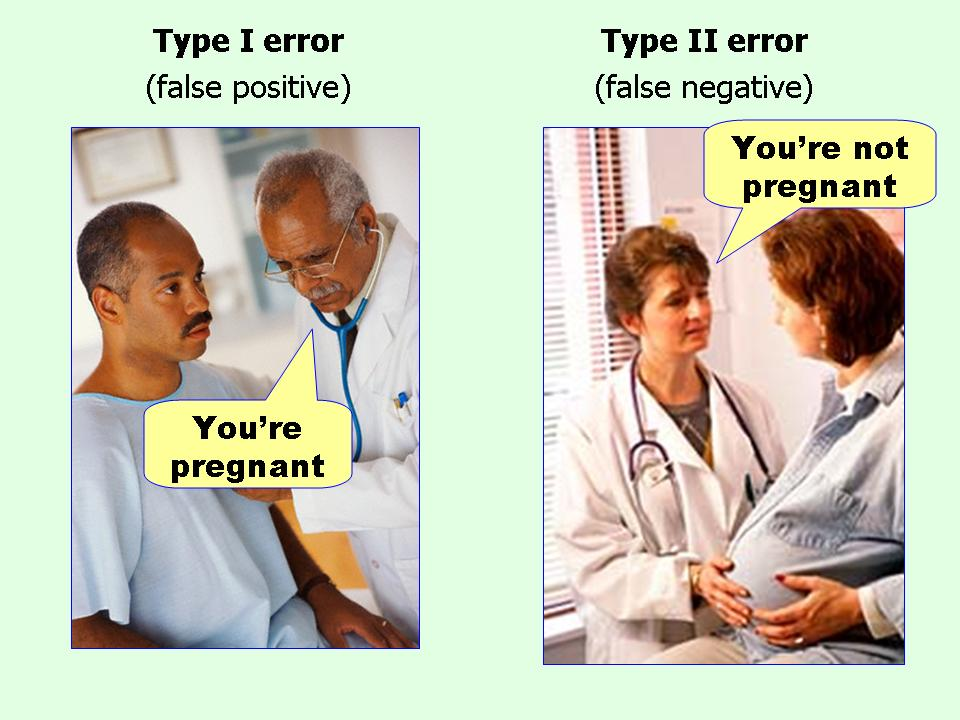
\includegraphics[width=1\linewidth]{images/type1type2error} 

}

\caption{Difference between Type 1 and Type 2 errors. Figure made by <a href="https://effectsizefaq.com/2010/05/31/i-always-get-confused-about-type-i-and-ii-errors-can-you-show-me-something-to-help-me-remember-the-difference/">Paul Ellis</a>}\label{fig:errortypes}
\end{figure}

So, for the next study you will perform, which of the four possible outcomes is most likely? First, let's assume you have set the alpha level to 5\%. Furthermore, let's assume you have designed a study so that it will have 80\% power (and for this example, let's assume Omniscient Jones knows you indeed have exactly 80\% power). The last thing to specify is the probability that the null hypothesis is true. Let's assume for this next study you have no idea if the null hypothesis is true or not, and that it is equally likely that the null hypothesis is true, or the alternative hypothesis is true (both have a probability of 50\%). We can now calculate what the most likely outcome of such a study is.

Before we perform this calculation, take a moment to think if you know the answer. You might have designed studies with a 5\% alpha level and 80\% power, where you believed it was equally likely that H0 or H1 was true. Surely, it is useful to have reasonable expectations about which result to expect, when we perform such a study? Yet in my experience, many researchers perform without thinking about these probabilities at all. They often hope to observe a true positive, even when in the situation described above, the most likely outcome is a true negative. Let's now calculate these probabilities.

Let's assume we perform 200 studies with a 5\% alpha level, 80\% power, and a 50\% probability that H0 is true. How many false positives, true positives, false negatives, and true negatives should we expect in the long run?

\begin{longtable}[]{@{}
  >{\raggedright\arraybackslash}p{(\columnwidth - 4\tabcolsep) * \real{0.3922}}
  >{\raggedright\arraybackslash}p{(\columnwidth - 4\tabcolsep) * \real{0.3072}}
  >{\raggedright\arraybackslash}p{(\columnwidth - 4\tabcolsep) * \real{0.3007}}@{}}
\toprule
\begin{minipage}[b]{\linewidth}\raggedright
\end{minipage} & \begin{minipage}[b]{\linewidth}\raggedright
H0 True (50\%)
\end{minipage} & \begin{minipage}[b]{\linewidth}\raggedright
H1 True (50\%)
\end{minipage} \\
\midrule
\endhead
Significant Finding (Positive result) α = 5\%, 1-β=80\% & \textbf{False Positive 5\%*50\%=2.5\% (5 studies)} & \textbf{True Positive 80\%*50\%=40\% (80 studies)} \\
Non-Significant Finding (Negative result) 1-α = 95\%, β=20\% & \textbf{True Negative 95\%*50\%=47.5\% (95 studies)} & \textbf{False Negative 20\%*50\%=10\% (20 studies)} \\
\bottomrule
\end{longtable}

In the table above we see that 2.5\% of all studies will be a false positive (a 5\% Type 1 error rate,
multiplied by a 50\% probability that H0 is true). 40\% of all studies will be a true positive (80\% power multiplied by a 50\% probability that H1 is true). The probability of a false negative is 10\% (a 20\% Type 2 error rate multiplied by a 50\% probability that H1 is true). The most likely outcome is a true negative, with 47.5\% (a 95\% probability observing a non-significant result, multiplied by a 50\% probability that H0 is true).

It might be that you are not too enthusiastic about this outlook, and you would like to perform studies that have a higher probability of observing a true positive. What should we do? We can reduce the alpha level, increase the power, or increase the probability that H1 is true. As the probability of observing a true positive depends on the power, multiplied by the probability that H1 is true, we should design studies where both of these values are high. Statistical power can be increased by changes in the design of the study (e.g., by increasing the sample size). The probability that H1 is true depends on the hypothesis you are testing. If the probability that H1 is true is very high from the outset, you are at the risk of testing a hypothesis that is already established with enough certainty. A solution, which might not happen that often in your career, is to come up with the test of a hypothesis that is not trivial, but that after explaining it to peers makes a lot of sense. In other words, they would not have come up with the idea themselves, but after explaining it to them, they think it is extremely plausible. Such creative research ideas will most likely be very rare in your academic career, if you ever have any at all. Not all research needs to be this ground-breaking. It is also extremely valuable to perform \textbf{replication and extension studies} where it is relatively likely that H1 is true, but the scientific community still benefits from knowing that findings generalize to different circumstances.

\hypertarget{positive-predictive-value}{%
\section{Positive predictive value}\label{positive-predictive-value}}

John Ioannides wrote a well known article titled ``Why Most Published Research Findings Are False'' \citep{ioannidis_why_2005}. At the same time, we have learned that if you set your alpha at 5\%, the Type 1 error rate will not be higher than 5\% (in the long run). How are these two statements related? Why aren't 95\% of published research findings true? They key to understanding this difference is that two different probabilities are calculated. The Type 1 error rate is the probability of saying there is an effect, when there is no effect. Ioannides calculates the \emph{positive predictive value} (PPV), which is the conditional probability that if a study turns out to show a statistically significant result, there is actually a true effect. This probability is useful to understand, because people often selectively focus on significant results, and because due to publication bias, in some research areas only significant results are published.

A real-life example where it was useful to understand the concept of the positive predictive value concerned the number of vaccinated and vaccinated people admitted to the hospital with COVID symptoms. In some places equal numbers of patients were vaccinated as unvaccinated. If you do not understand the concept of a positive predictive value, you might believe this reveals that it is equally likely to end up in the hospital, whether you are vaccinated or not. This is incorrect. As Figure \ref{fig:ppvhospital} nicely vizualizes, the probability that is person is vaccinated is very high, and the probability that a vaccinated person ends up in the hospital is much lower than the probability that an unvaccinated person ends up in the hospital. However, if we select only those individuals who end up in the hospital, we are computing a probability \emph{conditional} on being in the hospital.

\begin{figure}

{\centering 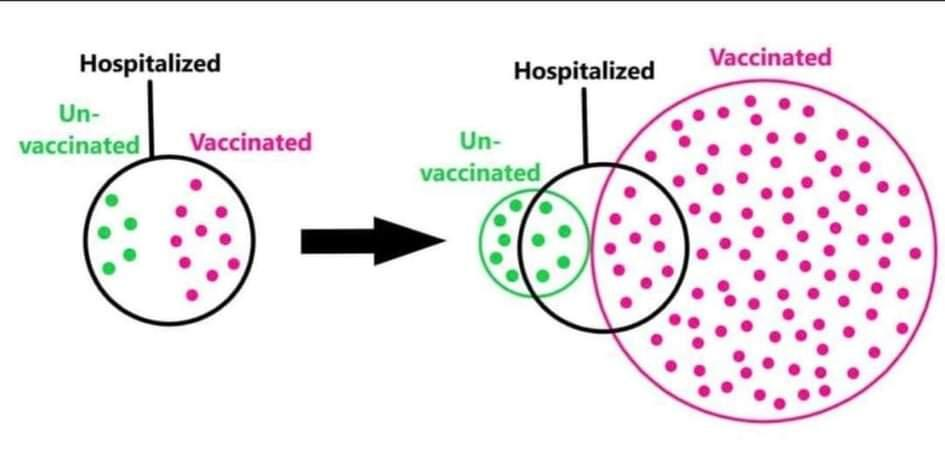
\includegraphics[width=1\linewidth]{images/hospitalvaccinated} 

}

\caption{Why there are more vaccinated people in the hospital.}\label{fig:ppvhospital}
\end{figure}

It is useful to understand what the probability is that, if you have observed a significant result in an experiment, the result is actually a true positive. In other words, in the long run, how many \emph{true positives} can we expect, among all positive results (both true positives and false positives)? This is known as the Positive Predictive Value (PPV). We can also calculate how many \emph{false positives} we can expect, among all positive results (again, both true positives and false positives). This is known as the \textbf{False Positive Report Probability} \citep{wacholder_assessing_2004}, sometimes also referred to as the False Positive Risk \citep{colquhoun_false_2019}.

\[PPV = \frac{\text{True}\ \text{Positives}}{(\text{True}\ \text{Positives} +
                                                \text{False}\ \text{Positives})}\]

\[FPRP = \frac{\text{False}\ \text{Positives}}{(\text{True}\ \text{Positives}
                                                  + \text{False}\ \text{Positives})}\]

The PPV and FPRP combine classic Frequentist concepts of statistical power and alpha levels with prior probabilities that H0 and H1 are true. They depend on the proportion of studies you do where there is an effect (H1 is true), and where there is no effect (H0 is true), in addition to the statistical power, and the alpha level. After all, you can only observe a false positive if the null hypothesis is true, and you can only observe a true positive if the alternative hypothesis is true. Whenever you perform a study, you are either operating in a reality where there is a true effect, or you are operating in a reality where there is no effect -- but you don't know in which reality you are.

When you perform studies, you will be aware of all outcomes of your studies (both the significant and the non-significant findings). When you read the literature, there is publication bias, and you often only have access to significant results. This is when thinking about the PPV (and the FPRP) becomes important. If we set the alpha level to 5\%, in the long run 5\% of studies where H0 is true (FP + TN) will be significant. But in a literature with only significant results, we do not have access to all true negatives, and it is
possible that the proportion of false positives in the literature is much larger than 5\%.

If we continue the example above, we see there are 85 positive results (80 + 5) in the 200 studies. The false positive report probability is 5/85 = 0.0588. At the same time, the alpha of 5\% guarantees that (in the long run) 5\% of the 100 studies where the null hypothesis is true are Type 1 errors: 5\%*100 = 0.05. This is also true. When we do 200 studies, at most 0.05*200 = 10 could possibly be false positives (if H0 was true in all experiments). In the 200 studies we performed (and where H0 was true in only 50\% of the studies), the \textbf{proportion of false positives for all experiments} is only 2.5\%. Thus, for all experiments you do, the proportion of false positives will, in the long run, never be higher than the Type I error rate set by the researcher (e.g., 5\% when H0 is true in all experiments), but it can be lower (when H0 is true in less than 100\% of the experiments).

\begin{figure}

{\centering 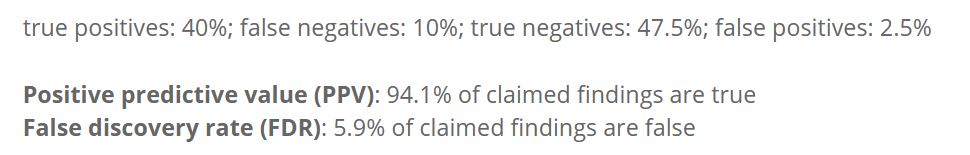
\includegraphics[width=1\linewidth]{images/PPVexample} 

}

\caption{Screenshot of the output of the results of the PPV Shiny app by <a href="http://shinyapps.org/apps/PPV/">Michael Zehetleitner and Felix Schönbrodt </a>}\label{fig:ppvexample}
\end{figure}

\emph{(Note: The FDR and FPRP are different abbreviations for the same thing)}

People often say something like: ``\emph{Well, we all know 1 in 20 results in the published literature are Type 1 errors}''. You should be able to understand this is not true in practice, after learning about the positive predictive value. It also explains why the common \emph{p}-value \protect\hyperlink{misconception4}{misconception} ``If you have observed a significant finding, the probability that you have made a Type 1 error (a false positive) is 5\%.'' is not correct. Even when we use a 5\% alpha level, it is quite reasonable to assume much more than 5\% of significant findings in the published literature are false positives. When in 100\% of the studies you perform, the null hypothesis is true, and all studies are published, only \emph{then} 1 in 20 studies, in the long run, are false positives (and the rest correctly reveal no statistically significant difference). In the scientific literature, the positive predictive value can be quite high, and under specific circumstances, it might even be so high that most published research findings are false. This will happen when researchers examine mostly studies where the null-hypothesis is true, with low power, or when the Type 1 error rate is inflated due to \emph{p}-hacking or other types of bias.

\hypertarget{type-1-error-inflation}{%
\section{Type 1 error inflation}\label{type-1-error-inflation}}

\begin{figure}

{\centering 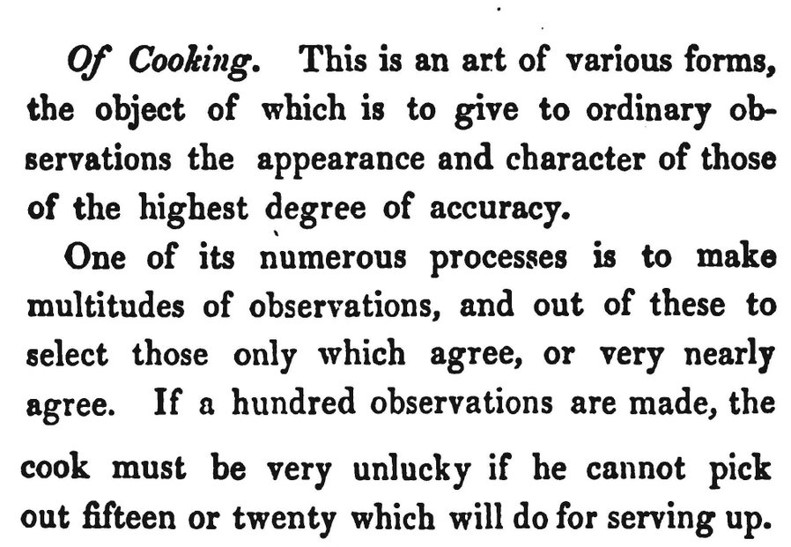
\includegraphics[width=1\linewidth]{images/babbagecooking} 

}

\caption{Quote from the 1830 book by Babbage Reflections on the Decline of Science in England And on Some of Its Causes available <a href="https://www.gutenberg.org/files/1216/1216-h/1216-h.htm">here</a>}\label{fig:cooking}
\end{figure}

If you perform multiple comparisons, there is a risk that the Type 1 error rate inflates. When multiple comparisons are planned, in some cases it is possible to control the Type 1 error rate by lowering the alpha level for each individual analysis. The most widely known approach to control for multiple comparisons is the Bonferroni correction where the alpha level is divided by the number of tests that is performed \citep{dunn_multiple_1961}. However, researchers also often use informal data analysis strategies that inflate the Type 1 error rate. Babbage \citeyearpar{babbage_reflections_1830} already complained about these problematic practices in 1830, and two centuries later, they are still common. Barber \citeyearpar{barber_pitfalls_1976} provides an in depth discussion of a range of approaches, such as eyeballing the data to decide which hypotheses to test (sometimes called `double dipping'), selectively reporting only those analyses that confirm predictions, and ignoring non-significant results, collecting many variables and performing multitudes of tests, or performing sub-group analyses when the planned analysis yields nonsignificant results, or after a nonsignificant prediction derive a new hypothesis that is supported by the data, and test the hypothesis on the data that the hypothesis was derived from (sometimes called HARKing \citep{kerr_harking_1998}). Many researchers admit to having used practices that inflate error rates \citep{fiedler_questionable_2015, john_measuring_2012, van_de_schoot_use_2021, chin_questionable_2021, makel_both_2021}. I myself have used such practices in the first scientific article I published, before I was fully aware of how problematic this was - for an article we published several years later in which we reflect on this, see \citet{jostmann_short_2016}.

For some paradigms, researchers have a lot of flexibility in how to compute the main dependent variable. Elson and colleagues examined 130 publications that use the Competitive Reaction Time Task, in which participants select the duration and intensity of blasts to be delivered to a competitor \citep{elson_press_2014}. The task is used to measure `aggressive behavior' in an ethical manner. To compute the score, researchers can use the duration of a noise blast, the intensity, or a combination therefore, averaged over any number of trials, with several possible transformations of the data. The 130 publications examined reported 157 different quantification strategies in total, showing that most calculations of the dependent variable were unique, used only in a single article. One might wonder why the same authors sometimes use different computations across articles. One possible explanation is that they used this flexibility in the data analysis to find statistically significant results.

\begin{figure}

{\centering 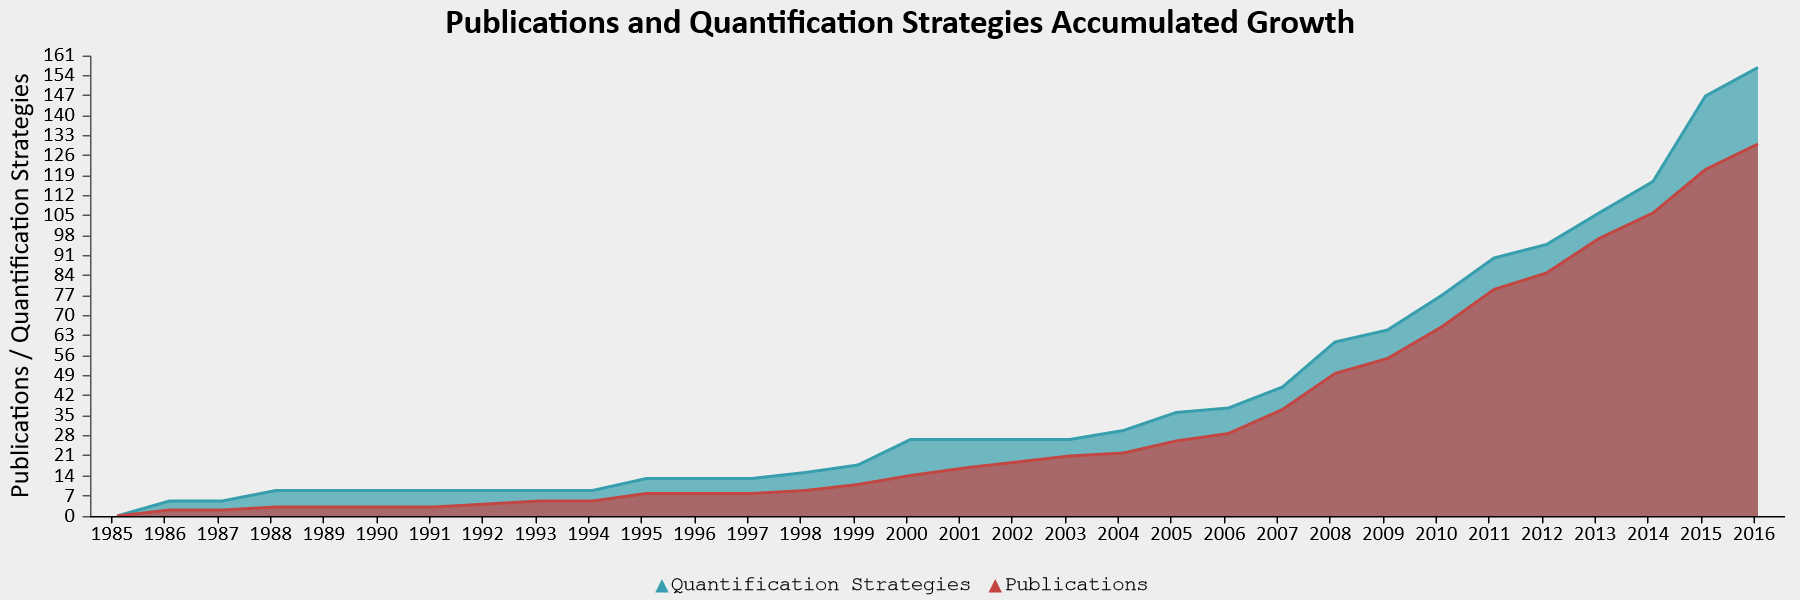
\includegraphics[width=1\linewidth]{images/flexiblemeasure} 

}

\caption{Plot of publications using CRTT (blue) and unique quantifications of the meaure (red). Figure from FlexibleMeasures.com by <a href="https://www.flexiblemeasures.com/crtt/index.php?menu=quantifications">Malte Elson</a>}\label{fig:flexiblemeasure}
\end{figure}

\hypertarget{optional-stopping}{%
\section{Optional stopping}\label{optional-stopping}}

\begin{figure}

{\centering 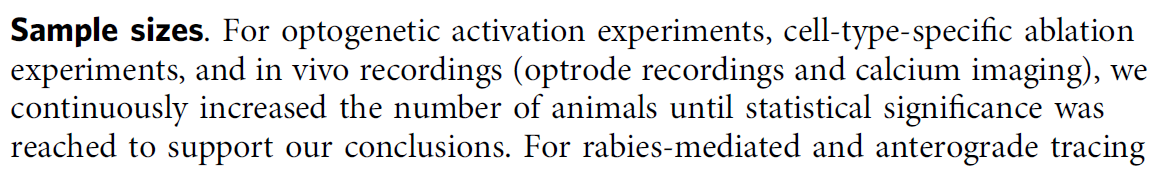
\includegraphics[width=1\linewidth]{images/optionalstoppingexample} 

}

\caption{Screenshot a scientific paper explicitly admitting to using optional stopping}\label{fig:optionalstoppingexample}
\end{figure}

One practice that inflates the Type 1 error rate is known as \textbf{optional stopping}. In optional stopping, a researcher repeatedly analyzes the data, continues the data collection when the test result is not statistically significant, but stops when a significant effect is observed. The quote from a published article in the figure above is an example where researchers transparently report they used optional stopping, but more commonly people do not disclose the use of optional stopping in their methods sections. Over the last years, many researchers have learned that optional stopping is problematic. This has in some lead to the general idea that you should not collect data, look at whether the results are significant, and stop data collection when the result is significant, or if not, continue data collection. That is not the correct conclusion, and is an example of becoming too inflexible. The correct approach to collect data in batches, called \textbf{sequential analysis}, has been extensively developed by statisticians, and is used in many studies. For example, the safety and efficacy of the Pfizer--BioNTech COVID-19 vaccine used an experimental design where they planned to analyze the data 5 times, and controlled the overall Type 1 error rate by lowering the alpha level for each interim analysis.

\begin{figure}

{\centering 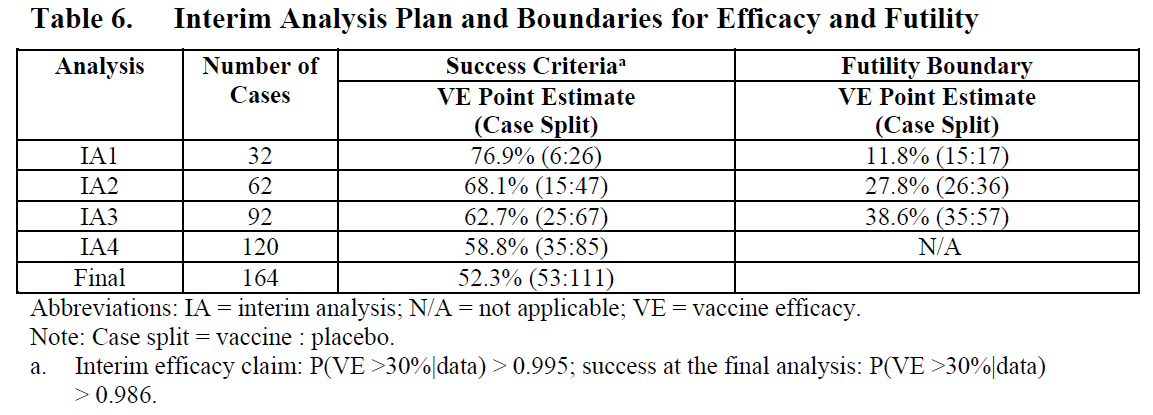
\includegraphics[width=1\linewidth]{images/vaccinetrial} 

}

\caption{Screenshot of the <a href="https://www.nejm.org/doi/suppl/10.1056/NEJMoa2034577/suppl_file/nejmoa2034577_protocol.pdf">planned interim analyses</a> examining the safety and Efficacy of the BNT162b2 mRNA Covid-19 Vaccine.}\label{fig:interim}
\end{figure}

The main lesson is that certain research practices can increase the flexibility and efficiency of studies you perform, when done right, but the same practices can inflate the Type 1 error rate when done wrong. Let's therefore try to get a better understanding when we are inflating our Type 1 error rate with optional stopping, and how to do this correctly using sequential analysis.

Copy the code below into R and run it. This script will simulate an ongoing data collection. After 10 participants in each condition, a \emph{p}-value is calculated by performing an independent \emph{t}-test, and this \emph{t}-test is then repeated after every additional participant that is collected. Then, all these \emph{p}-values are plotted as a function of the increasing sample size.

\begin{Shaded}
\begin{Highlighting}[]
\NormalTok{n }\OtherTok{\textless{}{-}} \DecValTok{200} \CommentTok{\# total number of datapoints (per condition) after initial 10}
\NormalTok{d }\OtherTok{\textless{}{-}} \FloatTok{0.0} \CommentTok{\# effect size d}

\NormalTok{p }\OtherTok{\textless{}{-}} \FunctionTok{numeric}\NormalTok{(n) }\CommentTok{\# store p{-}values}
\NormalTok{x }\OtherTok{\textless{}{-}} \FunctionTok{numeric}\NormalTok{(n) }\CommentTok{\# store x{-}values}
\NormalTok{y }\OtherTok{\textless{}{-}} \FunctionTok{numeric}\NormalTok{(n) }\CommentTok{\# store y{-}values}

\NormalTok{n }\OtherTok{\textless{}{-}}\NormalTok{ n }\SpecialCharTok{+} \DecValTok{10} \CommentTok{\# add 10 to number of datapoints}

\ControlFlowTok{for}\NormalTok{ (i }\ControlFlowTok{in} \DecValTok{10}\SpecialCharTok{:}\NormalTok{n) \{ }\CommentTok{\# for each simulated participants after the first 10}
\NormalTok{  x[i] }\OtherTok{\textless{}{-}} \FunctionTok{rnorm}\NormalTok{(}\AttributeTok{n =} \DecValTok{1}\NormalTok{, }\AttributeTok{mean =} \DecValTok{0}\NormalTok{, }\AttributeTok{sd =} \DecValTok{1}\NormalTok{)}
\NormalTok{  y[i] }\OtherTok{\textless{}{-}} \FunctionTok{rnorm}\NormalTok{(}\AttributeTok{n =} \DecValTok{1}\NormalTok{, }\AttributeTok{mean =}\NormalTok{ d, }\AttributeTok{sd =} \DecValTok{1}\NormalTok{)}
\NormalTok{  p[i] }\OtherTok{\textless{}{-}} \FunctionTok{t.test}\NormalTok{(x[}\DecValTok{1}\SpecialCharTok{:}\NormalTok{i], y[}\DecValTok{1}\SpecialCharTok{:}\NormalTok{i], }\AttributeTok{var.equal =} \ConstantTok{TRUE}\NormalTok{)}\SpecialCharTok{$}\NormalTok{p.value}
\NormalTok{\}}

\NormalTok{p }\OtherTok{\textless{}{-}}\NormalTok{ p[}\DecValTok{10}\SpecialCharTok{:}\NormalTok{n] }\CommentTok{\# Remove first 10 empty p{-}values}

\CommentTok{\# Create the plot}
\FunctionTok{plot}\NormalTok{(}\DecValTok{0}\NormalTok{, }\AttributeTok{col =} \StringTok{"red"}\NormalTok{, }\AttributeTok{lty =} \DecValTok{1}\NormalTok{, }\AttributeTok{lwd =} \DecValTok{3}\NormalTok{, }\AttributeTok{ylim =} \FunctionTok{c}\NormalTok{(}\DecValTok{0}\NormalTok{, }\DecValTok{1}\NormalTok{), }\AttributeTok{xlim =} \FunctionTok{c}\NormalTok{(}\DecValTok{10}\NormalTok{, n), }
     \AttributeTok{type =} \StringTok{"l"}\NormalTok{, }\AttributeTok{xlab =} \StringTok{"sample size"}\NormalTok{, }\AttributeTok{ylab =} \StringTok{"p{-}value"}\NormalTok{)}
\FunctionTok{lines}\NormalTok{(p, }\AttributeTok{lwd =} \DecValTok{2}\NormalTok{)}
\FunctionTok{abline}\NormalTok{(}\AttributeTok{h =} \FloatTok{0.05}\NormalTok{, }\AttributeTok{col =} \StringTok{"darkgrey"}\NormalTok{, }\AttributeTok{lty =} \DecValTok{2}\NormalTok{, }\AttributeTok{lwd =} \DecValTok{2}\NormalTok{) }\CommentTok{\# draw line at p = 0.05}

\FunctionTok{min}\NormalTok{(p) }\CommentTok{\# Return lowest p{-}value from all looks}
\FunctionTok{cat}\NormalTok{(}\StringTok{"The lowest p{-}value was observed at sample size"}\NormalTok{, }\FunctionTok{which.min}\NormalTok{(p) }\SpecialCharTok{+} \DecValTok{10}\NormalTok{) }
\FunctionTok{cat}\NormalTok{(}\StringTok{"The p{-}value dropped below 0.05 for the first time at sample size:"}\NormalTok{, }
    \FunctionTok{ifelse}\NormalTok{(}\FunctionTok{is.na}\NormalTok{(}\FunctionTok{which}\NormalTok{(p }\SpecialCharTok{\textless{}} \FloatTok{0.05}\NormalTok{)[}\DecValTok{1}\NormalTok{] }\SpecialCharTok{+} \DecValTok{10}\NormalTok{), }\StringTok{"NEVER"}\NormalTok{, }\FunctionTok{which}\NormalTok{(p }\SpecialCharTok{\textless{}} \FloatTok{0.05}\NormalTok{)[}\DecValTok{1}\NormalTok{] }\SpecialCharTok{+} \DecValTok{10}\NormalTok{)) }
\end{Highlighting}
\end{Shaded}

For example, in the Figure below, you see the \emph{p}-value plotted on the y-axis (from 0 to 1) and the sample size plotted on the x-axis (from 0 to 200). For this simulation, the true effect size was d = 0, meaning there is no true effect. We can thus only observe true negatives or false positives. As the sample size increases, the \emph{p}-value slowly moves up and down (remember from the chapter on \protect\hyperlink{pvalues}{\emph{p}-values} that when there is no true effect, \emph{p}-values are uniformly distributed). In Figure \ref{fig:animatep}, the \emph{p}-value drops below the grey line (indicating an alpha level 0.05) after collecting 83 participants in each condition, only to drift back upwards to larger \emph{p}-values. From this figure, if becomes clear that the more often we look at the data, and the larger the total sample size, the higher the probability that one of the analyses will yield a p \textless{} \(\alpha\). If resources are infinite, the Type 1 error rate will be 1, and a researcher can always find a significant result through optional stopping.

\begin{figure}

{\centering \animategraphics[width=1\linewidth,controls,loop]{100}{02-errorcontrol_files/figure-latex/animatep-}{1}{210}

}

\caption[Simulated *p*-values for each additional observation when the null is true]{Simulated *p*-values for each additional observation when the null is true.}\label{fig:animatep}
\end{figure}

When there \emph{is} a true effect, we see that \emph{p}-values also vary, but they will eventually drop to below the alpha level. Due to the variation, we just do not know exactly when. When we perform an a-priori power analysis, we can compute the probability that looking at a specific sample size will yield a significant \emph{p}-value. In Figure \ref{fig:animatep2} we see the same simulation, but now when there is a true but small effect of d = 0.3. With 200 observations per condition, a sensitivity power analysis reveals that we have 85\% power. If we would analyze the data at an interim analysis (e.g., after 150 observations) we would often already find a statistically significant effect (as we would have 74\% power). This illustrates a benefit of sequential analyses, where we control error rates, but can stop early at an interim analysis. Sequential analyses are especially useful in large or expensive studies where there is uncertainty about the true effect size.

\begin{figure}

{\centering \animategraphics[width=1\linewidth,controls,loop]{100}{02-errorcontrol_files/figure-latex/animatep2-}{1}{210}

}

\caption[Simulated *p*-values for each additional observation when d = 0.3]{Simulated *p*-values for each additional observation when d = 0.3.}\label{fig:animatep2}
\end{figure}

Let's more formally examine the inflation of the Type 1 error rate through optional stopping in a \textbf{simulation study}. Copy the code below into R and run the code. Note that the 50000 simulations (needed to get the error rates reasonably accurate) take some time to run.

\begin{Shaded}
\begin{Highlighting}[]
\NormalTok{N }\OtherTok{\textless{}{-}} \DecValTok{100} \CommentTok{\# total datapoints (per condition)}
\NormalTok{looks }\OtherTok{\textless{}{-}} \DecValTok{5} \CommentTok{\# set number of looks at the data}
\NormalTok{nsims }\OtherTok{\textless{}{-}} \DecValTok{50000} \CommentTok{\# number of simulated studies}
\NormalTok{alphalevel }\OtherTok{\textless{}{-}} \FloatTok{0.05} \CommentTok{\# set alphalevel}

\NormalTok{look\_at\_n }\OtherTok{\textless{}{-}} \FunctionTok{ceiling}\NormalTok{(}\FunctionTok{seq}\NormalTok{(N }\SpecialCharTok{/}\NormalTok{ looks, N, (N }\SpecialCharTok{{-}}\NormalTok{ (N }\SpecialCharTok{/}\NormalTok{ looks)) }\SpecialCharTok{/}\NormalTok{ (looks}\DecValTok{{-}1}\NormalTok{))) }\CommentTok{\# looks}
\NormalTok{look\_at\_n}\OtherTok{\textless{}{-}}\NormalTok{look\_at\_n[look\_at\_n }\SpecialCharTok{\textgreater{}} \DecValTok{2}\NormalTok{] }\CommentTok{\#Remove looks at N of 1 or 2}
\NormalTok{looks}\OtherTok{\textless{}{-}}\FunctionTok{length}\NormalTok{(look\_at\_n) }\CommentTok{\#if looks are removed, update number of looks}

\NormalTok{matp }\OtherTok{\textless{}{-}} \FunctionTok{matrix}\NormalTok{(}\ConstantTok{NA}\NormalTok{, }\AttributeTok{nrow =}\NormalTok{ nsims, }\AttributeTok{ncol =}\NormalTok{ looks) }\CommentTok{\# Matrix for p{-}values l tests}
\NormalTok{p }\OtherTok{\textless{}{-}} \FunctionTok{numeric}\NormalTok{(nsims) }\CommentTok{\# Variable to save pvalues}

\CommentTok{\# Loop data generation for each study, then loop to perform a test for each N}
\ControlFlowTok{for}\NormalTok{ (i }\ControlFlowTok{in} \DecValTok{1}\SpecialCharTok{:}\NormalTok{nsims) \{}
\NormalTok{  x }\OtherTok{\textless{}{-}} \FunctionTok{rnorm}\NormalTok{(}\AttributeTok{n =}\NormalTok{ N, }\AttributeTok{mean =} \DecValTok{0}\NormalTok{, }\AttributeTok{sd =} \DecValTok{1}\NormalTok{)}
\NormalTok{  y }\OtherTok{\textless{}{-}} \FunctionTok{rnorm}\NormalTok{(}\AttributeTok{n =}\NormalTok{ N, }\AttributeTok{mean =} \DecValTok{0}\NormalTok{, }\AttributeTok{sd =} \DecValTok{1}\NormalTok{)}
  \ControlFlowTok{for}\NormalTok{ (j }\ControlFlowTok{in} \DecValTok{1}\SpecialCharTok{:}\NormalTok{looks) \{}
\NormalTok{    matp[i, j] }\OtherTok{\textless{}{-}} \FunctionTok{t.test}\NormalTok{(x[}\DecValTok{1}\SpecialCharTok{:}\NormalTok{look\_at\_n[j]], y[}\DecValTok{1}\SpecialCharTok{:}\NormalTok{look\_at\_n[j]], }
                         \AttributeTok{var.equal =} \ConstantTok{TRUE}\NormalTok{)}\SpecialCharTok{$}\NormalTok{p.value }\CommentTok{\# perform the t{-}test, store}
\NormalTok{  \}}
  \FunctionTok{cat}\NormalTok{(}\StringTok{"Loop"}\NormalTok{, i, }\StringTok{"of"}\NormalTok{, nsims, }\StringTok{"}\SpecialCharTok{\textbackslash{}n}\StringTok{"}\NormalTok{)}
\NormalTok{\}}

\CommentTok{\# Save Type 1 error rate smallest p at all looks}
\ControlFlowTok{for}\NormalTok{ (i }\ControlFlowTok{in} \DecValTok{1}\SpecialCharTok{:}\NormalTok{nsims) \{}
\NormalTok{  p[i] }\OtherTok{\textless{}{-}} \FunctionTok{ifelse}\NormalTok{(}\FunctionTok{length}\NormalTok{(matp[i,}\FunctionTok{which}\NormalTok{(matp[i,] }\SpecialCharTok{\textless{}}\NormalTok{ alphalevel)]) }\SpecialCharTok{==} \DecValTok{0}\NormalTok{, }
\NormalTok{                 matp[i,looks], matp[i,}\FunctionTok{which}\NormalTok{(matp[i,] }\SpecialCharTok{\textless{}}\NormalTok{ alphalevel)])}
\NormalTok{\}}

\FunctionTok{hist}\NormalTok{(p, }\AttributeTok{breaks =} \DecValTok{100}\NormalTok{, }\AttributeTok{col =} \StringTok{"grey"}\NormalTok{) }\CommentTok{\# create plot}
\FunctionTok{abline}\NormalTok{(}\AttributeTok{h =}\NormalTok{ nsims }\SpecialCharTok{/} \DecValTok{100}\NormalTok{, }\AttributeTok{col =} \StringTok{"red"}\NormalTok{, }\AttributeTok{lty =} \DecValTok{3}\NormalTok{)}

\FunctionTok{cat}\NormalTok{(}\StringTok{"Type 1 error rates for look 1 to"}\NormalTok{, looks, }\StringTok{":"}\NormalTok{, }
    \FunctionTok{colSums}\NormalTok{(matp }\SpecialCharTok{\textless{}}\NormalTok{ alphalevel) }\SpecialCharTok{/}\NormalTok{ nsims)}
\FunctionTok{cat}\NormalTok{(}\StringTok{"Type 1 error rate when only the lowest p{-}value for all looks is reported:"}\NormalTok{, }
    \FunctionTok{sum}\NormalTok{(p }\SpecialCharTok{\textless{}}\NormalTok{ alphalevel) }\SpecialCharTok{/}\NormalTok{ nsims)}
\end{Highlighting}
\end{Shaded}

This simulation will perform multiple independent \emph{t}-tests on simulated data, looking multiple times until the maximum sample size is reached. In the first four lines, you can set the most important parameters of the simulation. First, the maximum sample size in each condition (e.g., 100). Then, the number of looks (e.g., 5). At best, you can look at the data after every participant (e.g., with 100 participants, you can look 100 times -- or actually 98 times, because you need more than 2 participants in each condition for a \emph{t}-test!). You can set the number of simulations (the more, the clearer the pattern will be, but the longer the simulation takes), and the alpha level (e.g., 0.05). Since you can only make a Type 1 error when there is no true effect, the effect size is set to 0 in these simulations.

When you perform only a single test, the Type 1 error rate is the probability of finding a \emph{p}-value lower than your alpha level, when there is no effect. In an optional stopping scenario where you look at the data twice, the Type 1 error rate is the probability of finding a \emph{p}-value lower than your alpha level at the first look, \textbf{and} the probability of \textbf{not} finding a \emph{p}-value lower than your alpha level at the \textbf{first} look, but finding a \emph{p}-value lower than your alpha level at the \textbf{second} look. This is a \emph{conditional probability}, which makes error control a little bit more complex than when multiple looks are completely independent.

So how much does optional stopping inflate the Type 1 error rate? And which \emph{p}-values can we expect under optional stopping?

Start by running the simulation without changing any values, so simulating 100 participants in each condition, looking 5 times at your data, with an alpha of 0.05. Note the 50.000 simulations take a while! You should see something similar to Figure \ref{fig:optionalstopfig} below (which is based on 500.000 simulations to make the pattern very clear).

\textbackslash begin\{figure\}

\{\centering 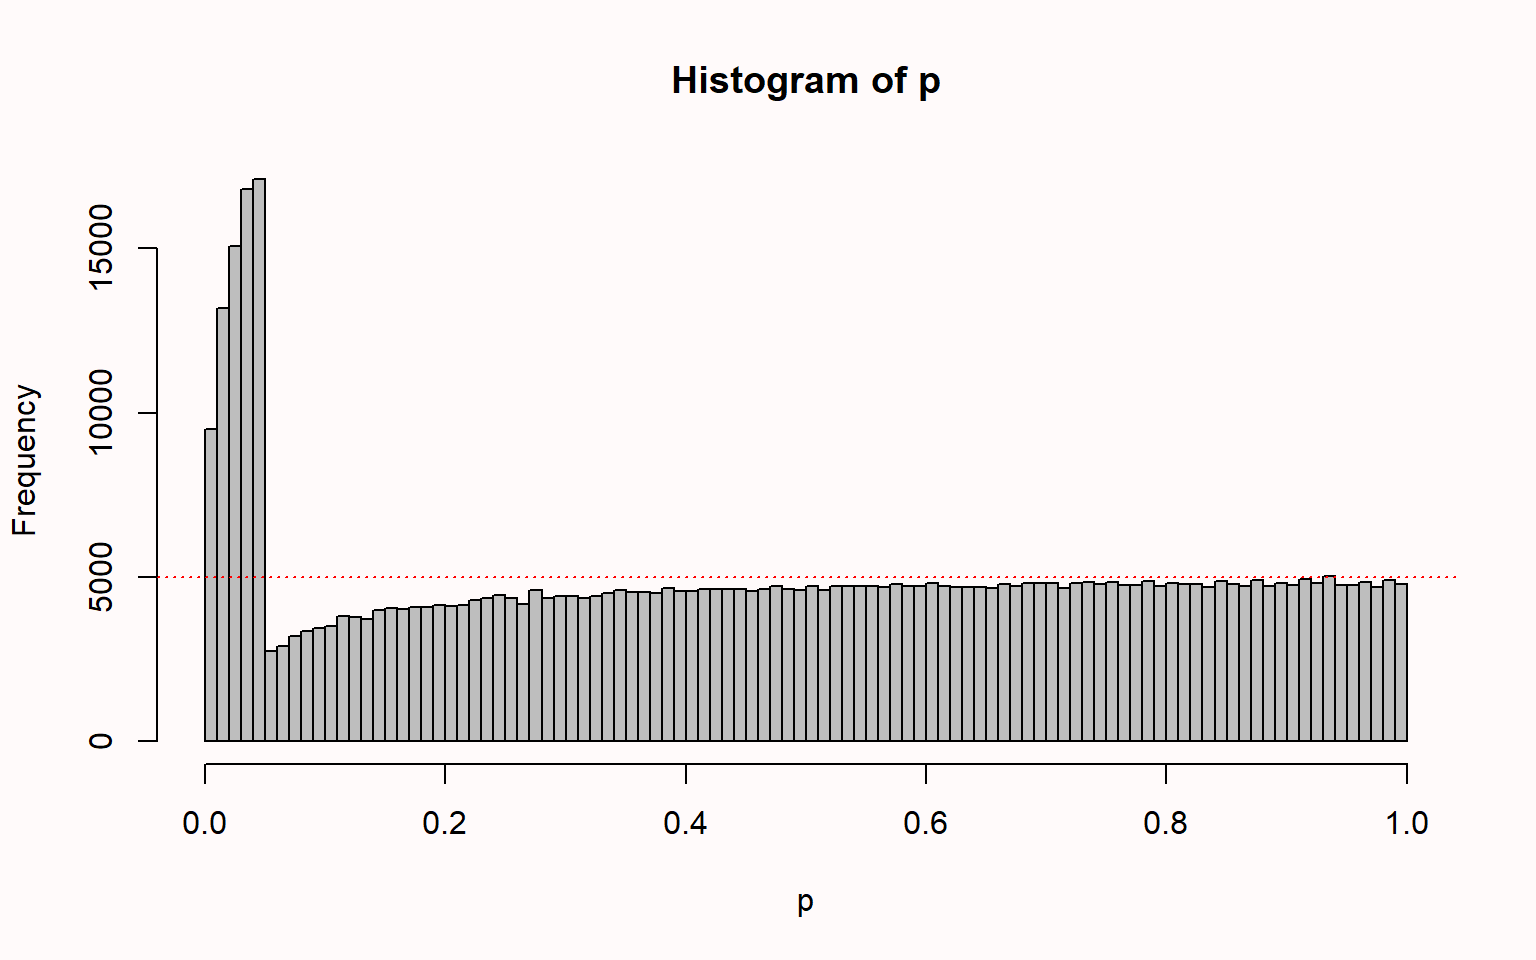
\includegraphics[width=1\linewidth]{02-errorcontrol_files/figure-latex/optionalstopfig-1}

\}

\textbackslash caption\{Simulation of 500000 studies performing 5 interim analyses at an alpha level of 5\%\}\label{fig:optionalstopfig}
\textbackslash end\{figure\}

We see 100 bars, one for each \% (so one for all \emph{p}-values between 0.00 and 0.01, one for \emph{p}-values between 0.01 and 0.02, etc.). There is a horizontal line that indicates where all \emph{p}-values should fall, is they would be uniformly distributed (as they should be when there is no true effect, as explained in the chapter on \protect\hyperlink{pvalues}{\emph{p}-values}).

The distribution of \emph{p}-values is peculiar. We see that compared to a uniform distributions, a bunch of results just above the alpha threshold of 0.05 are missing, and they seem to have been pulled just below 0.05, where there is a much higher frequency of outcomes compared to when data is not analyzed multiple times as it comes in. Notice how relatively high \emph{p}-values (e.g., \emph{p} = 0.04) are more common than lower \emph{p}-values (e.g., 0.01). We will see in the chapter on \href{bias}{bias detection} that statistical techniques such as \emph{p}-curve analysis can pick up on this pattern.

When using an alpha level of 5\% with 5 looks at the data, the overall Type 1 error rate has inflated to 14\%. If we lower the alpha level at each interim analysis, the overall Type 1 error rate can be controlled. The shape of the \emph{p}-value distribution will still look peculiar, but the total number of significant test results will be controlled at the desired alpha level. The well-known Bonferroni correction (i.e., using an alpha level of \(\alpha\) / the number of looks), but the \href{https://en.wikipedia.org/wiki/Pocock_boundary}{Pocock correction} is slighlty more efficient. For more information on how to perform interim analyses while controlling error rates, see the dedicated chapter on \protect\hyperlink{sequential}{sequential analysis}.

\hypertarget{justifyerrorrate}{%
\section{Justifying Error Rates}\label{justifyerrorrate}}

\begin{quote}
If we reject H0 , we may reject it when it is true; if we accept H0 , we may be accepting it when it is false, that is to say, when really some alternative Bt is true. These two sources of error can rarely be eliminated completely; in some cases it will be more important to avoid the first, in others the second. We are reminded of the old problem considered by LaplaceE of the number of votes in a court of judges that should be needed to convict a prisoner. Is it more serious to convict an innocent man or to acquit a guilty? That will depend upon the consequences of the error ; is the punishment death or fine ; what is the danger to the community of released criminals ; what are the current ethical views on punishment? From the point of view of mathematical theory all that we can do is to show how the risk of the errors may be controlled and minimised. The use of these statistical tools in any given case, in determining just how the balance should be struck, must be left to the investigator.
\end{quote}

Even though in \emph{theory} the Type 1 and Type 2 error rate should be justified by the researcher, as Neyman and Pearson \citeyearpar{neyman_problem_1933} write above, in \emph{practice} researchers tend to imitate others. The default use of an alpha level of 0.05 can already be found in work\} of Gosset on the \emph{t}-distribution \citep{cowles_origins_1982, kennedy-shaffer_before_2019}, who believed that a difference of two standard deviations (a z-score of 2) was sufficiently rare. The default use of 80\% power (or a 20\% Type 2 error rate) is similarly based on personal preferences by \citet{cohen_statistical_1988}, who writes:

\begin{quote}
It is proposed here as a convention that, when the investigator has no other basis for setting the desired power value, the value .80 be used. This means that beta is set at .20. This value is offered for several reasons (Cohen, 1965, pp.~98-99). The chief among them takes into consideration the implicit convention for alpha of .05. The beta of .20 is chosen with the idea that the general relative seriousness of these two kinds of errors is of the order of .20/.05, i.e., that Type I errors are of the order of four times as serious as Type II errors. This .80 desired power convention is offered with the hope that it will be ignored whenever an investigator can find a basis in his substantive concerns in his specific research investigation to choose a value ad hoc.
\end{quote}

We see that conventions are built on conventions: the norm to aim for 80\% power is built on the norm to set the alpha level at 5\%. Although there is nothing special about an alpha level of 5\%, it is interesting to reflect on why it has become so widely established. \citet{uygun_tunc_epistemic_2021} argue that one possible reason is that, as far as conventions go, an alpha level of 5\% might be low enough such that peers take any claims made with this error rate seriously, while at the same time being high enough such that peers will be motivated to perform an independent replication study to increase or decrease our confidence in the claim. Although lower error rates would establish claims more convincingly, this would also require more resources. One might speculate
that in research areas where not every claim is important enough to a careful justification of costs and benefits, 5\% has a pragmatic function in facilitating conjectures and refutations in fields that otherwise lack a coordinated approach to knowledge generation, but are faced with limited resources.

Nevertheless, some researchers have proposed to move away from the default use of a 5\% alpha level. For example, \citet{johnson_revised_2013} proposes a default significance level of 0.005 or 0.001. Others have cautioned against such blanket recommendation because the additional resources required to reduce the Type 1 error rate might not be worth the costs \citep{lakens_justify_2018}. A lower alpha lever requires a larger sample size to achieve the same sstatistical power. If the sample size can not be increased, a lower alpha level reduces the statistical power, and increases the Type 2 error rate. Whether that is desireable should be evaluated on a case by case basis.

There are two main reasons to abandon the universal use of a 5\% alpha level. The first reason to carefully choose an alpha level is that decision-making becomes more efficient \citep{mudge_setting_2012}. If researchers use hypothesis tests to make dichotomous decisions from a methodological falsificationist approach to statistical inferences, and have a certain maximum sample size they are willing or able to collect, it is typically possible to make decisions more efficiently by choosing error rates such that the combined cost of Type 1 and Type 2 errors is minimized. If we aim to either minimize or balance Type 1 and Type 2 error rates for a given sample size and effect size, the alpha level should be set not based on convention, but by weighting the relative cost of both types of errors \citep{maier_justify_2022}.

For example, imagine a researcher plans to collect 64 participants per condition to detect a d = 0.5 effect, and weighs the cost of Type 1 errors 4 times as much as Type 2 errors. This is exactly the scenario Cohen (1988) described, and with 64 participants per condition the relative weigfht of Type 1 and Type 2 errors yields a 5\% Type 1 error rate and a 20\% Type 2 error rate. Now imagine this researchers realizes they have the resources to collect 80 observations instead of just 64. With an interest in an effect size of d = 0.5, the relative weight of Type 1 and Type 2 errors of 4 would be satisfied when they set the alpha level to 0.037 as then the the Type 2 error rate is 0.147. Alternatively, the researcher might have decided to collect 64 observations, but not balance the error rates, but set the alpha level such that the weighted combined error rate is minimized, which is achieved when the alpha level is set to 0.033, as vizualized in Figure \ref{fig:minimizeerror} (for further information, see \citet{maier_justify_2022}).

\begin{figure}

{\centering 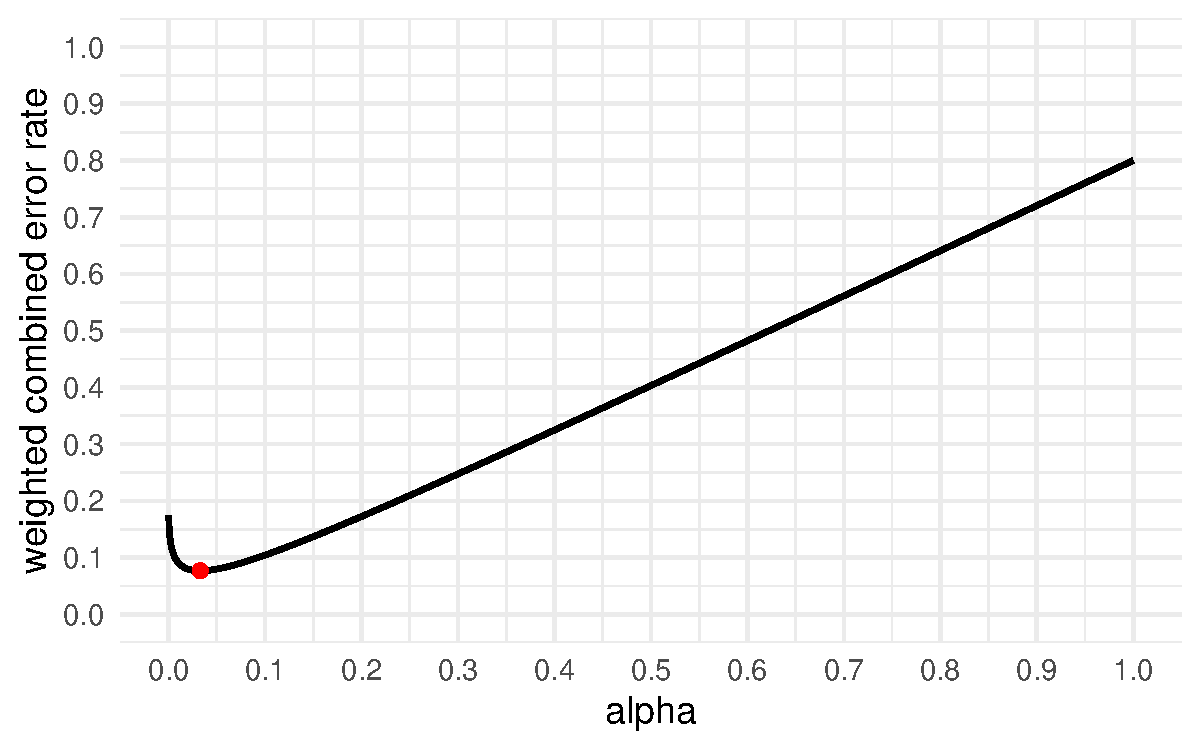
\includegraphics[width=1\linewidth]{02-errorcontrol_files/figure-latex/minimizeerror-1} 

}

\caption{Weighted combined error rate, minimized at alpha = 0.037.}\label{fig:minimizeerror}
\end{figure}

Justifying error rates can leads to situations where the alpha level is increased above 0.05, because this leads to more optimal decision making. Winer (1962) writes: ``The frequent use of the .05 and .01 levels of significance is a
197 matter of convention having little scientific or logical basis. When the power of tests is likely to be low under these levels of significance, and when Type 1 and Type 2 errors are of approximately equal importance, the .30 and .20 levels of significance may be more appropriate than the .05 and .01 levels.'' The reasoning here is that a design that has 70\% power for the smallest effect size of interest would not balance the Type 1 and Type 2 error rates in a sensible manner. Of course, such an increase An increase of the alpha level should only be deemed acceptable when authors can justify that the costs of the increase in the Type 1 error rate is sufficiently compensated by the benefit of decreased Type 2 error rate. This will encompass cases where (1) the study will have practical implications that require decision making, (2) a cost-benefit analysis is provided that gives a clear rationale for relatively high costs of a Type 2 error, (3) the probability that H1 is false is relatively low, and (4) it is not feasible to blackuce overall error rates by collecting more data.

One should also carefully reflect on the choice of the alpha level when an experiment achieves very high statistical power for all effect sizes that are considered meaningful. If a study has 99\% power for effect sizes of interest, and thus a 1\% Type 2 error rate, but uses the default 5\% alpha level, it also suffers from a lack of balance, and the use of a lower alpha level would lead to a more balanced decision, and increase the severity of the test.

The second reason is most relevant for large data sets, and is related to \protect\hyperlink{lindley}{Lindley's paradox}. As the statistical power increases, some \emph{p}-values below 0.05 (e.g., \emph{p} = 0.04) can be more likely when there is \emph{no} effect than when there \emph{is} an effect. To prevent situations where a frequentist rejects the null hypothesis based on \emph{p} \textless{} 0.05, when the evidence in the test favors the null hypothesis over the alternative hypothesis, it is recommended to lower the alpha level as a function of the sample size. The need to do so is discussed by \citet{leamer_specification_1978}, who writes ``The rule of thumb quite popular now, that is, setting the significance level arbitrarily to .05, is shown to be deficient in the sense that from every reasonable viewpoint the significance level should be a decreasing function of sample size.'' The idea of this approach is to reduce the alpha level such that a Bayes factor or likelihood computed for the a significant results would never be evidence \emph{for} the null hypothesis (for an online Shiny app to perform such calculations, see \href{https://shiny.ieis.tue.nl/JustifyAlpha/}{here} or the app below).

\begin{center}\href{https://shiny.ieis.tue.nl/JustifyAlpha/}{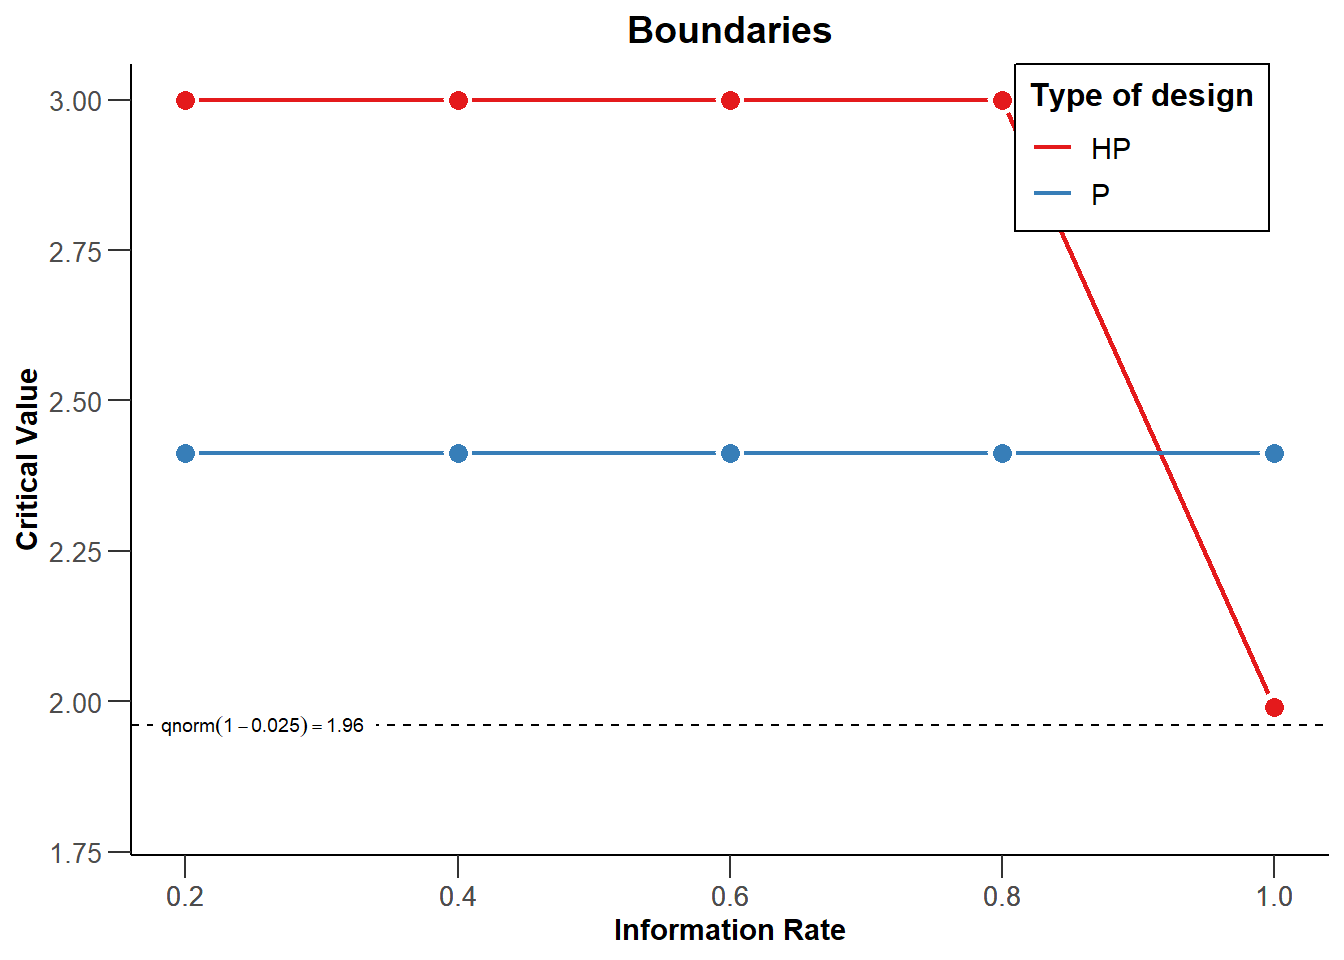
\includegraphics[width=1\linewidth]{02-errorcontrol_files/figure-latex/unnamed-chunk-5-1} }\end{center}

\hypertarget{multiplecomparisons}{%
\section{Why you don't need to adjust your alpha level for all tests you'll do in your lifetime.}\label{multiplecomparisons}}

Some researchers criticize corrections for multiple comparisons because one might as well correct for all tests you do in your lifetime {[}\citet{perneger_whats_1998}. If you choose to use a Neyman-Pearson approasch to statistics the only reason to correct for all tests you perform in your lifetime is when all the work you have done in your life tests a single theory, and you would use your last words to decide to accept or reject this theory, as long as only one of all individual tests you have performed yielded a p \textless{} α. Researchers rarely work like this.

Instead, in a Neyman-Pearson approach to hypothesis testing, the goal is to use data to make decisions about how to act. Neyman \citep{neyman_inductive_1957} calls his approach \textbf{inductive behavior}. The outcome of an experiment leads one to take different possible actions, which can be either practical (e.g., implement a new procedure, abandon a research line) or scientific (e.g., claim there is or is no effect). From an error-statistical approach \citep{mayo_statistical_2018} inflated Type 1 error rates mean that it has become very likely that you will be able to claim support for your hypothesis, even when the hypothesis is wrong. This reduces the severity of the test. To prevent this, we need to control our error rate at the level of our claim.

A useful distinction in the literature on multiple testing is a \textbf{union-intersection} testing approach, and a \textbf{intersection-union} testing approach \citep{dmitrienko_traditional_2013}. In a union-intersection approach, a claim is made when \emph{at-least-one} test is significant. In these cases, a correction for multiple comparisons is required to control the error rate. In a intersection-union approach, a claim is made when all performed tests are statistically significant, and no correction for multiple comparisons is required (and indeed, under some assumptions researchers could even \emph{increase} the alpha level in a intersection-union approach).

It might seem if researchers can get out of corrections for multiple comparisons by formulating a hypothesis for every possible test they will perform. Indeed, they can. For a ten by ten correlation matrix, a researcher might state they are testing 45 unique predictions, each at an uncorrected alpha level. However, readers might reasonably question whether these 45 tests were predicted by a theory, and if only a few of the 45 tests show a significant result, the meager track record of the predictions should make us doubt the theory they were derived from. There are different ways to control for error rates, the easiest being the Bonferroni correction an the ever-so-slightly less conservative Holm-Bonferroni sequential procedure. When the number of statistical tests becomes substantial, it is sometimes preferable to control false discovery rates, instead of error rates \citep{benjamini_controlling_1995}.

\hypertarget{power-analysis}{%
\section{Power Analysis}\label{power-analysis}}

So far we have largely focused on Type 1 error control. As was clear from Figure \ref{fig:animatep2}, when there is a true effect \emph{p}-values will eventually become smaller than an alpha level as the sample size becomes large enough. When designing an experiment the goal is to choose a sample size that provides a desired Type 2 error rate for an effect size of interest. This can be achieved by performing an a-priori power analysis. It is important to highlight that the goal of an a-priori power analysis is \emph{not} to achieve sufficient power for the true effect size. The true effect size is always unknown when designing a study. The goal of an a-priori power analysis is to achieve sufficient power, given a specific \emph{assumption} of the effect size a researcher wants to detect. Just like a Type I error rate is the maximum probability of making a Type I error conditional on the assumption that the null hypothesis is true, an a-priori power analysis is computed under the assumption of a specific effect size. It is unknown if this assumption is correct. All a researcher can do is to make sure their assumptions are well justified. Statistical inferences based on a test where the Type II error is controlled are conditional on the assumption of a specific effect size. They allow the inference that, assuming the true effect size is at least as large as that used in the a-priori power analysis, the maximum Type II error rate in a study is not larger than a desired value.

In Figure \ref{fig:powerd} we see the expected distribution of observed standardized effect sizes (Cohen's d) for an independent \emph{t}-test with 50 observations in each condition. The bell-shaped curve on the left represents the expectations if the null is true, and the red areas in the tail represent Type 1 errors. The bell-shaped curve on the right represents the expectations if the alternative hypothesis is true, and d= 0.5. The vertical line at d = 0.4 represents the \textbf{critical effect size}. With this sample size and an alpha level of 0.05, observed effect sizes smaller than d = 0.4 will not be statistically significant. If there is a true effect, these outcomes will be Type 2 errors, illustrated by the blue shaded area. The remainder of the curve reflects true positives, when there is a true effect, and the observed effect sizes is statistically significant. The power of the test is the percentages of the distribution on the right that is larger than the critical value.

\begin{figure}

{\centering 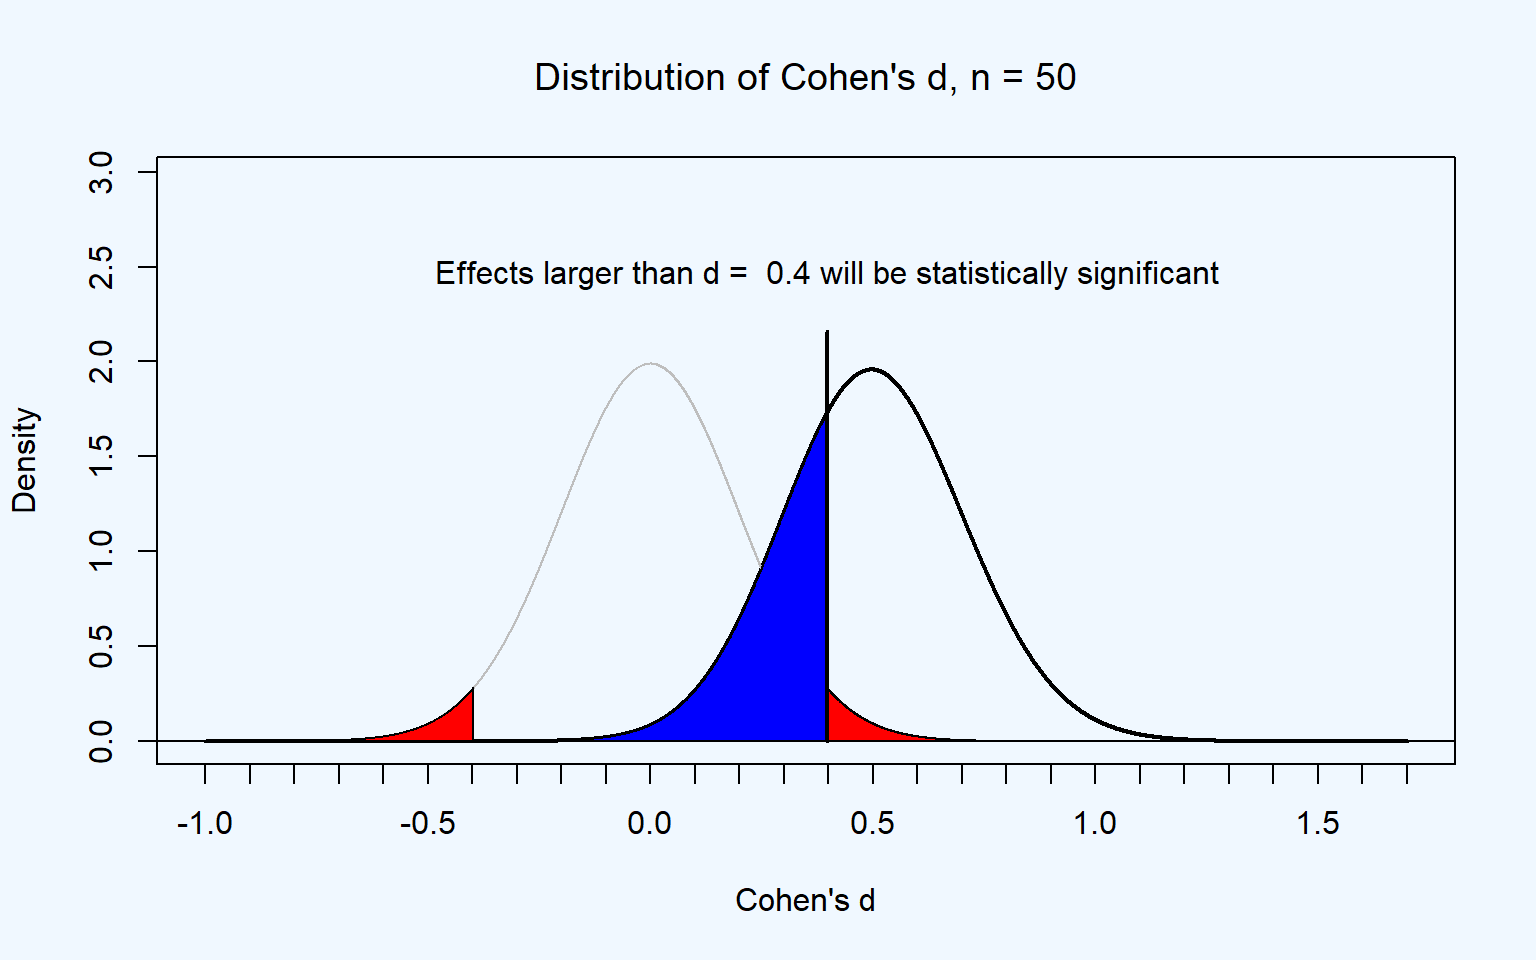
\includegraphics[width=1\linewidth]{02-errorcontrol_files/figure-latex/powerd-1} 

}

\caption{Distribution of d = 0 and d = 0.5 for an independent *t*-test with n = 50.}\label{fig:powerd}
\end{figure}

The issue of Type 2 error control will be discussed in more detail i nthe chapter on sample size justification. Even thought the topic of Type 2 error control is only briefly discussed here, it is at least as important as Type 1 error control. An informative study should have a high probability of observing an effect if there is an effect. Indeed, the default recommendation to aim for 80\% power leaves a surprisingly large (20\%) probability of a Type 2 error. If a researcher only cares about not making a decision error, but the researcher does not care about whether this decision error is a false positive or a false negative, an argument could be made that Type 1 and Type 2 errors are weighed equally. Therefore, desiging a study with balanced error rates (e.g., a 5\% Type 1 error and 95\% power) would make sense.

\hypertarget{test-yourself-1}{%
\section{Test Yourself}\label{test-yourself-1}}

\hypertarget{questions-about-the-positive-predictive-value}{%
\subsection{Questions about the positive predictive value}\label{questions-about-the-positive-predictive-value}}

\textbf{Q1}: In the example at the start of this chapter, we see that we control the Type 1 error rate at 5\% by using an alpha of 0.05. Still, when there is a 50\% probability that H0 is true, the proportion of false positives for all experiments performed turns out to be much lower, namely 2.5\%, or 0.025. Why?

\begin{enumerate}
\def\labelenumi{\Alph{enumi})}
\tightlist
\item
  The proportion of false positives for all experiments we have performed is a variable with a distribution around the true error rate -- sometimes it's higher, sometimes it's lower, due to random variation.
\item
  The proportion of false positives for all experiments we have performed is only 5\% when H0 is true for all 200 studies.
\item
  The proportion of false positives for all experiments we have performed is only 5\% when you have 50\% power -- if power increases above 50\%, the proportion of false positives for all experiments we have performed becomes smaller.
\item
  The proportion of false positives for all experiments we have performed is only 5\% when you have 100\% power, and it becomes smaller if power is lower than 100\%.
\end{enumerate}

\textbf{Q2}: What will make the biggest difference in improving the probability that you will find a true positive? Check your answer by shifting the sliders in the online PPV app.

\begin{enumerate}
\def\labelenumi{\Alph{enumi})}
\tightlist
\item
  Increase the \% of a-priori true hypotheses
\item
  Decrease the \% of a-priori true hypotheses
\item
  Increase the alpha level
\item
  Decrease the alpha level
\item
  Increase the power
\item
  Decrease the power
\end{enumerate}

Increasing the power requires bigger sample sizes, or studying larger effects. Increasing the \% of a-priori true hypotheses can be done by making better predictions -- for example building on reliable findings, and relying on strong theories. These are useful recommendations if you want to increase the probability of performing studies where you find a statistically significant result.

\textbf{Q3}: Set the ``\% of a priori true hypotheses'' slider to 50\%. Leave the `α level' slider at 5\%. Leave the `\% of p-hacked studies' slider at 0. The title of Ioannidis' paper is `why most published research findings are false'. One reason might be that studies often have low power. At which value for power is the PPV 50\%. In other words, at which level of power is a significant result just as likely to be true, as that it is false?

\begin{enumerate}
\def\labelenumi{\Alph{enumi})}
\tightlist
\item
  80\%
\item
  50\%
\item
  20\%
\item
  5\%
\end{enumerate}

It seems low power alone is not the best explanation for why most published findings might be false, as it is unlikely that power is low enough in the scientific literature. Ioannidis (2005) discusses some scenarios under which it becomes likely that most published research findings are false. Some of these assume that `p-hacked studies', or studies that show a significant result due to bias, enter the literature. There are good reasons to believe this happens, as we discussed in this chapter. In the `presets by Ioannidis' dropdown menu, you can select some of these situations. Explore all of them, and pay close attention to the ones where the PPV is smaller than 50\%.

\textbf{Q4}: In general, when are most published findings false? Interpret `low' and `high' in the answer options below in relation to the values in the first example in this chapter of 50\% probability H1 is true, 5\% alpha, 80\% power,
and 0\% bias.

\begin{enumerate}
\def\labelenumi{\Alph{enumi})}
\tightlist
\item
  When the probability of examining a true hypothesis is low, combined with either low power or substantial bias (e.g., p-hacking).
\item
  When the probability of examining a true hypothesis is high, combined with either low power or substantial bias (e.g., p-hacking).
\item
  When the alpha level is high, combined with either low power or substantial bias (e.g., p-hacking).
\item
  When power is low and p-hacking is high (regardless of the \% of true hypotheses one examines).
\end{enumerate}

\textbf{Q5}: Set the ``\% of a priori true hypotheses'' slider to 0\%. Set the ``\% of p-hacked studies'' slider to 0\%. Set the ``α level'' slider to 5\%. Play around with the power slider. Which statement is true?
\textbf{Without \emph{p}-hacking, when the alpha level is 5\%, and when 0\% of the hypotheses are true, }

\begin{enumerate}
\def\labelenumi{\Alph{enumi})}
\tightlist
\item
  the proportion of false positives for all experiments we have performed is 100\%.
\item
  the PPV depends on the power of the studies.
\item
  regardless of the power, the PPV equals the proportion of false positives for all experiments we have performed.
\item
  regardless of the power, the proportion of false positives for all experiments we have performed is 5\%, and the PPV is 0\% (all significant results are false positives).
\end{enumerate}

\hypertarget{questions-about-optional-stopping}{%
\subsection{Questions about optional stopping}\label{questions-about-optional-stopping}}

\textbf{Q1}: Run the script that plots the \emph{p}-value as the sample size increases 20 times, and count how often the lowest \emph{p}-value ends up below 0.05 (we will calculate the long run probability of this happening through more extensive simulations later).

\textbf{Q2}: If there is a true effect, we can only observe a true positive or a false negative. Change the effect size from d \textless- 0.0 to d \textless- 0.3. This is a relatively small true effect, and with 200 participants in each condition, we have 85\% power (or an 85\% probability of finding a significant effect). Run the script again. Below is one possible example of the trajectory of \emph{p}-values as the sample size increases. Run the script 20 times. Take a good look at the variation in the \emph{p}-value trajectory. Remember that at N = 200, 85\% of the times the \emph{p}-value should have ended up below 0.05. The script returns the sample size the \emph{p}-value is the lowest (which is often, but not always, at the maximum sample size, when there is a true effect) and the sample size at which the \emph{p}-value drops below 0.05 for the first time. Which statement is true?

\begin{enumerate}
\def\labelenumi{\Alph{enumi})}
\tightlist
\item
  If the \emph{p}-value drops below 0.05, it stays below 0.05.
\item
  The \emph{p}-value randomly moves between 0 and 1, and will every now and then end up below 0.05.
\item
  The \emph{p}-value often drops below 0.05 well before 200 participants in each
  condition. In around 50\% of the simulations, this already happens at N = 100.
\item
  The \emph{p}-value will typically move below 0.05 and stay there for some time,
  but given a large enough sample, it will always move back up to \emph{p} \textgreater{} 0.05.
\end{enumerate}

\textbf{Q3}: Change the effect size d \textless- 0.8, which can be regarded as a large effect. Run the script 20 times. Take a good look at the variation in the \emph{p}-value trajectory. Which statement is true?

\begin{enumerate}
\def\labelenumi{\Alph{enumi})}
\tightlist
\item
  The \emph{p}-value randomly moves between 0 and 1, and will every now and then end up below 0.05.
\item
  The \emph{p}-values drop below and stay below 0.05 much earlier than when the true effect size is 0.3.
\item
  \emph{p}-values are meaningful when effect sizes are large (e.g., d = 0.8), but meaningless when effect sizes are small (e.g., d = 0.3).
\item
  When you examine a large effect, whenever a \emph{p}-value drops below 0.05, it will always stay below 0.05 as the sample size increases.
\end{enumerate}

\textbf{Q4}: Looking at Figure \ref{fig:optionalstopfig}, which statement is true?

\begin{enumerate}
\def\labelenumi{\Alph{enumi})}
\tightlist
\item
  Optional stopping does not impact the Type 1 error rate.
\item
  Optional stopping inflates the Type 1 error rate. We can see this in the first five bars (\emph{p}-values between 0.00 and 0.05), which are substantially higher than the horizontal line.
\item
  Optional stopping inflates the Type 1 error rate. We can see this in the bars just above 0.05, which dip substantially below the uniform distribution that should be present if there is no true effect.
\end{enumerate}

\textbf{Q5}: The script to simulate optional stopping provides written output. One summary gives you the Type 1 error rate for each individual look. One summary gives the Type 1 error rate when optional stopping is used. When running the script with the default values, which statement is true?

\begin{enumerate}
\def\labelenumi{\Alph{enumi})}
\tightlist
\item
  At each look, the Type 1 error rate is higher than the alpha level (0.05).
  When using optional stopping (and reporting only the lowest \emph{p}-value), the Type 1 error rate is higher than 0.05.
\item
  At each look, the Type 1 error rate is approximately equal to the alpha level (0.05). When using optional stopping (and reporting only the lowest \emph{p}-value), the alpha level also approximately equals the alpha level (0.05).
\item
  At each look, the Type 1 error rate is approximately equal to the alpha level (0.05). When using optional stopping, the Type 1 error rate is also higher than the alpha level (0.05).
\end{enumerate}

\textbf{Q6}: Change the number of looks in the simulation to \textbf{2} (change `looks \textless- 5' to `looks \textless- 2'), and leave all other settings the same. Run the simulation again. What is the Type 1 error rate using optional stopping with only 1 interim analysis, rounded to 2 digits? (Note that due to small number of simulations, the exact alpha level you get might differ a little bit from the
answer options below).

\begin{enumerate}
\def\labelenumi{\Alph{enumi})}
\tightlist
\item
  0.05
\item
  0.08
\item
  0.12
\item
  0.18
\end{enumerate}

\textbf{Q7}: As Wagenmakers \citeyearpar{wagenmakers_practical_2007} notes: \emph{``a user of NHST could always obtain a significant result through optional stopping (i.e., analyzing the data as they accumulate and stopping the experiment whenever the p-value reaches some desired significance level)''}. This is correct. It's true that the \emph{p}-value will always drop below the alpha level at some point in time. But, we need a rather large number of observations. We can calculate the maximum Type 1 error rate due to optional stopping for any maximum sample size. For example, what is the maximum Type 1 error rate when optional stopping is used when collecting 200 participants in each condition, and looking 200 times (or 198 times, given that you can't perform a \emph{t}-test on a sample size of 1 or 2 people)? Set the number of participants to \textbf{200}, the number of looks to \textbf{200}, the number of simulations to \textbf{10000} (this simulation will take even longer!), and the alpha to \textbf{0.05}.

What is maximum Type 1 error rate when collecting 200 participants in each
condition of an independent \emph{t}-test, using optional stopping, rounded to 2
digits? (Note that the simulation will take a while, but still, due to the
relatively small number of simulations, the exact alpha level you get might
differ a little bit from the answer options below -- choose the answer option
closest to your result).

\begin{enumerate}
\def\labelenumi{\Alph{enumi})}
\tightlist
\item
  0.05
\item
  0.11
\item
  0.20
\item
  0.41
\end{enumerate}

\textbf{Q8}: At Wikipedia, look at the entry about the Pocock boundary: \url{https://en.wikipedia.org/wiki/Pocock_boundary} . There are ethical reasons to look at the data, while data is being collected. These are clear in medicine, but similar arguments can be made for other research areas (see Lakens, 2014). Researchers often want to look at the data multiple times. This is perfectly fine, as long as they design a study with a number of looks in advance, and control their Type 1 error rate.

The Pocock boundary provides a very easy way to control the type 1 error rate in sequential analyses. Sequential analysis is the formal way to do optional stopping. Researchers should use a slightly lower alpha level for each look, the make sure the overall alpha level (after all looks) is not larger than 5\%.

Set the number of participants to \textbf{100}, the number of looks to \textbf{5}, and
the number of simulations to \textbf{50000} (so back to the original script). In the Wikipedia article on the Pocock boundary, find the corrected alpha level for 5 looks at the data. Change the alpha level in the simulation to this value. Run the simulation. Which of the following statements is true?

\begin{enumerate}
\def\labelenumi{\Alph{enumi})}
\tightlist
\item
  The Type 1 error rate at each look is approximately 0.03, and the overall alpha level is approximately 0.05.
\item
  The Type 1 error rate at each look is approximately 0.03, and the overall alpha level is approximately 0.15.
\item
  The Type 1 error rate at each look is approximately 0.016, and the overall alpha level is approximately 0.05.
\item
  The Type 1 error rate at each look is approximately 0.016, and the overall alpha level is approximately 0.08.
\end{enumerate}

\textbf{Q9}: Look at the graph of the \emph{p}-value distribution when using the Pocock boundary, and compare it to the graph you got when not using the Pocock boundary. You can flip back and forth between plots you have generated in RStudio using the blue arrows on the plots tab. Which statement is true?

\begin{enumerate}
\def\labelenumi{\Alph{enumi})}
\tightlist
\item
  \textbf{Without} Pocock's boundary, \textbf{small} \emph{p}-values (e.g., \emph{p} = 0.01) are
  \textbf{more} likely than slightly \textbf{higher} \emph{p}-values (\emph{p} = 0.04). \textbf{With}
  Pocock's boundary, \textbf{small} \emph{p}-values (e.g., \emph{p} = 0.01) are \textbf{also more}
  likely than slightly \textbf{higher} \emph{p}-values (\emph{p} = 0.04).
\item
  \textbf{Without} Pocock's boundary, \textbf{small} \emph{p}-values (e.g., \emph{p} = 0.01) are
  \textbf{more} likely than slightly \textbf{higher} \emph{p}-values (\emph{p} = 0.04). \textbf{With}
  Pocock's boundary, \textbf{small} \emph{p}-values (e.g., \emph{p} = 0.01) are \textbf{less} likely
  than slightly \textbf{higher} \emph{p}-values (\emph{p} = 0.04).
\item
  \textbf{Without} Pocock's boundary, \textbf{small} \emph{p}-values (e.g., \emph{p} = 0.01) are
  \textbf{less} likely than slightly \textbf{higher} \emph{p}-values (\emph{p} = 0.04). \textbf{With}
  Pocock's boundary, \textbf{small} \emph{p}-values (e.g., \emph{p} = 0.01) are \textbf{more} likely
  than slightly \textbf{higher} \emph{p}-values (\emph{p} = 0.04).
\item
  \textbf{Without} Pocock's boundary, \textbf{small} \emph{p}-values (e.g., \emph{p} = 0.01) are
  \textbf{less} likely than slightly \textbf{higher} \emph{p}-values (\emph{p} = 0.04). \textbf{With}
  Pocock's boundary, \textbf{small} \emph{p}-values (e.g., \emph{p} = 0.01) are \textbf{also less}
  likely than slightly \textbf{higher} \emph{p}-values (\emph{p} = 0.04).
\end{enumerate}

\hypertarget{likelihoods}{%
\chapter{Likelihoods}\label{likelihoods}}

In addition to frequentist and Bayesian approaches to statistical inferences, likelihoods provide a third approach to statistical inferences \citep{pawitan_all_2001}. Unlike Bayesian approaches, likelihoodists do not incorporate prior into their inferences. As the likelihoodists Taper and Lele \citeyearpar{taper_philosophy_2011} write:

\begin{quote}
It is not that we believe that Bayes' rule or Bayesian mathematics is flawed, but that from the axiomatic foundational definition of probability Bayesianism is doomed to answer questions irrelevant to science. We do not care what you believe, we barely care what we believe, what we are interested in is what you can show.
\end{quote}

Unlike the Neyman-Pearson frequentist approach, likelihoodists are interested in quantifying relative evidence, and unlike the Fisherian frequentist approach, likelihoodists specify a null and an alternative model, and quantify the relative likelihood of the data under both models.

Likelihood approaches to statistical inferences form a bridge between frequentist approaches and Bayesian approaches, and are an independent third approach to statistical inferences. At the same time, likelihood functions are an important part of Neyman-Pearson statistics through the Neyman-Pearson lemma, which shows that the likelihood ratio test it the most powerful test of H0 against H1, and is useful in determining the critical value used to reject a hypothesis. In Bayesian approaches, the likelihood is combined with a prior to compute a posterior probability distribution.

We can use likelihood functions to make inferences about unknown quantities. Let's imagine you flip a coin 10 times, and it turns up heads 8 times. What is the true probability (which we will indicate by the Greek letter theta, p) of this coin landing on heads?

The \textbf{binomial probability} of observing \emph{x} successes in \emph{n} studies is:

\[
Pr\left( k;n, p \right) = \frac{n!}{k!\left( n - k \right)!}p^{k}{(1 - p)}^{n - k}
\]

where \emph{p} is the probability of a success, \emph{k} is the observed number of successes, and \emph{n} is the number of trials. The first term indicates the number of possible combinations of results (e.g., you could start out with eight successes, end with eight successes, or any of the other possible combinations), which is multiplied by the probability of observing one success in each of the trials, which is then multiplied by the probability of observing no success in the remaining trials.

Let's assume you expect this is a fair coin. What is the binomial probability of observing 8 heads out of 10 coin flips, when \emph{p} = 0.5? The answer is:

\[
Pr\left(0.5;8,10 \right) = \frac{10!}{8!\left( 10 - 8 \right)!}*0.5^{8}*{(1 - 0.5)}^{10 - 8}
\]
In R this probability is computed as as:

\begin{Shaded}
\begin{Highlighting}[]
\FunctionTok{factorial}\NormalTok{(}\DecValTok{10}\NormalTok{)}\SpecialCharTok{/}\NormalTok{(}\FunctionTok{factorial}\NormalTok{(}\DecValTok{8}\NormalTok{)}\SpecialCharTok{*}\NormalTok{(}\FunctionTok{factorial}\NormalTok{(}\DecValTok{10{-}8}\NormalTok{))) }\SpecialCharTok{*} \FloatTok{0.5}\SpecialCharTok{\^{}}\DecValTok{8} \SpecialCharTok{*}\NormalTok{ (}\DecValTok{1} \SpecialCharTok{{-}} \FloatTok{0.5}\NormalTok{)}\SpecialCharTok{\^{}}\NormalTok{(}\DecValTok{10{-}8}\NormalTok{)}
\end{Highlighting}
\end{Shaded}

or by using the function:

\begin{Shaded}
\begin{Highlighting}[]
\FunctionTok{dbinom}\NormalTok{(}\AttributeTok{x =} \DecValTok{2}\NormalTok{, }\AttributeTok{size =} \DecValTok{10}\NormalTok{, }\AttributeTok{prob =} \FloatTok{0.5}\NormalTok{)}
\end{Highlighting}
\end{Shaded}

Let's assume we don't have any other information about this coin. (You might believe most coins are fair; such priors will be discussed when we talk about \protect\hyperlink{bayes}{Bayesian statistics} in the next chapter). The equation \emph{Pr(k;n,p)} gives the probability of observing \emph{k} successes from \emph{n} trials when a coin's probability of success is \emph{p}. Based on the data we have observed, we can ask the question: which value of \emph{p} will make the observed data \textbf{most likely}? To answer this question, we can plug in the values for \emph{k} and \emph{n} and find which value of \emph{p} maximizes this function. \href{https://en.wikipedia.org/wiki/Ronald_Fisher}{Ronald Fisher} called this maximum likelihood estimation (this is considered one of the most important developments in 20th century statistics, and Fisher published his first paper on this in 1912 as a third year undergraduate when he was 22 \citep{aldrich_r_1997}). Since \emph{p} can be any value between 0 and 1, we can plot all values in what is known as the \emph{likelihood function}, so we can see the maximum more easily.

\begin{figure}

{\centering 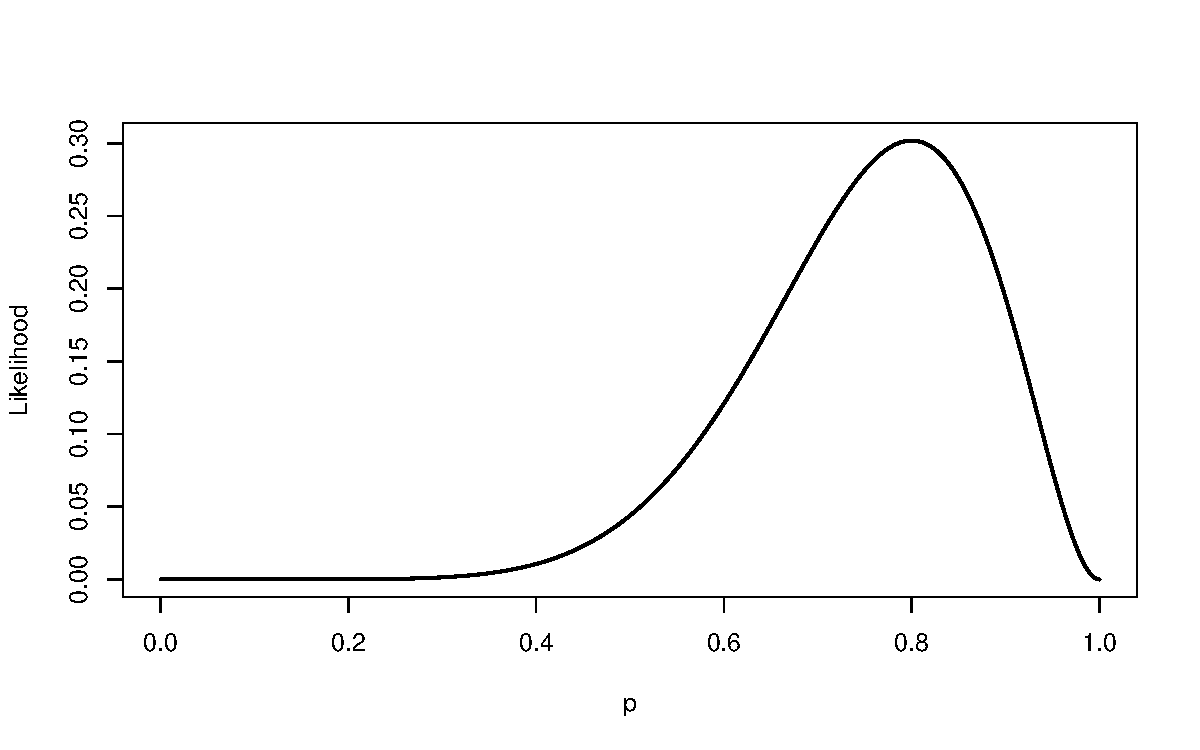
\includegraphics[width=1\linewidth]{03-likelihoods_files/figure-latex/like1-1} 

}

\caption{Binomial likelihood function for 8 successes in 10 trials.}\label{fig:like1}
\end{figure}

The likelihood \emph{Pr(k;n,p)} is plotted for all possible values of \emph{p} (from 0 to 1) It should not be surprising that given the data we have observed, the most likely value for the true parameter is 8 out of 10, or \emph{p} = 0.8, with a likelihood of 0.30 (the highest point on the y-axis). In this example, \emph{p} = 0.8 is called the \textbf{maximum likelihood estimator}. It is important to know that the likelihood itself has no meaning in isolation. In this sense, it differs from a probability. But we can compare likelihoods of the same function across different values of \emph{p}. You can read off any other value for any other θ, and see that given the observed data, low values of \emph{p} (e.g., 0.2) are not very likely.

Probabilities and likelihoods are related, but different. Note how the equation for Pr involves both information about the data (\emph{k}, \emph{n}) and information about the parameter (\emph{p}). To compute a \textbf{probability}, we view \emph{p} as fixed (for instance, for a fair coin, we plug in \emph{p} = 0.5) and then estimate the probability of different outcomes (\emph{k}, \emph{n}). The resulting function is the probability mass function. To compute the \textbf{likelihood}, we instead view the observed data as fixed (e.g., observing 5 heads out of 10 coin tosses), and we view Pr as a function of \emph{p}, estimating the value that maximizes the likelihood of a particular sample.

Likelihoods are an example of statistical inference: We have observed some data, and we use this data to draw an inference about different population parameters. More formally, the likelihood function is the (joint) density function evaluated at the observed data. Likelihood functions can be calculated for many different models (binomial distributions, normal distributions, see \citet{millar_maximum_2011}).

The likelihood curve rises up and falls down, except at the extremes, when 0 heads or only heads are observed. When we plot the likelihood curves for 0 heads in 10 coin flips, the likelihood curve looks like:

\begin{figure}

{\centering 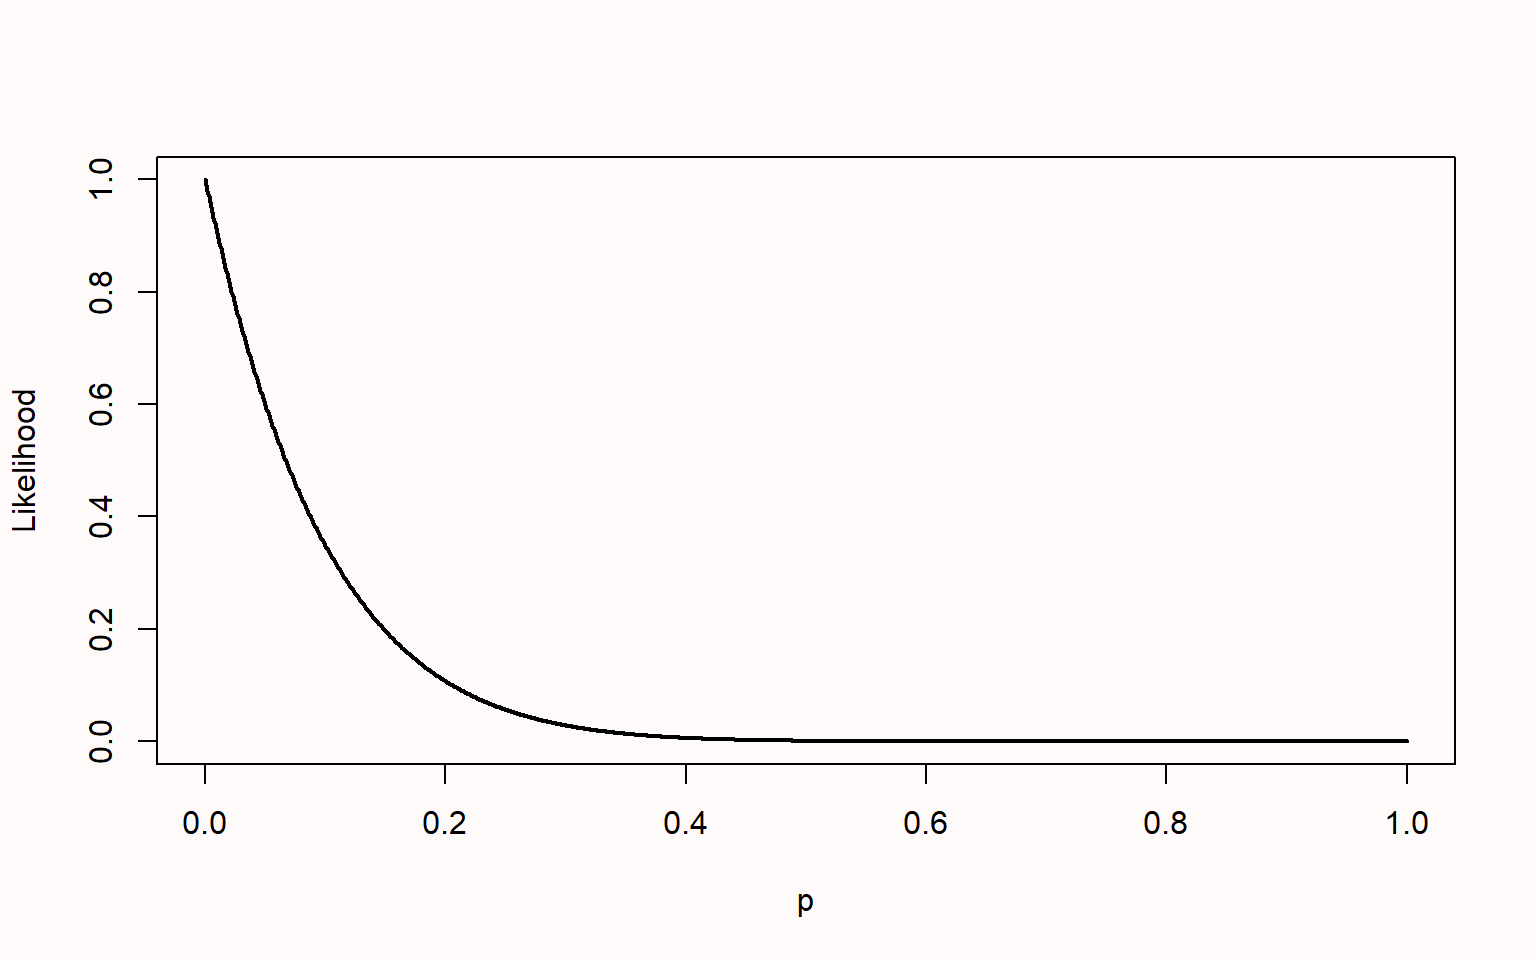
\includegraphics[width=1\linewidth]{03-likelihoods_files/figure-latex/like2-1} 

}

\caption{Binomial likelihood function for 0 successes in 10 trials.}\label{fig:like2}
\end{figure}

Likelihoods can easily be combined. Imagine we have two people flipping the same coin independently. One person observes eight heads out of 10 flips, and the other observes 4 heads out of 10 flips. You might believe that this should give the same likelihood curve as one person flipping a coin 20 times, and observing 12 heads, and indeed, it does. In the plot below, all likelihood curves are standardized by dividing the curve by the maximum of each likelihood curve. This is why all curves now have a maximum of 1, and we can more easily compare different likelihood curves.

\begin{figure}

{\centering 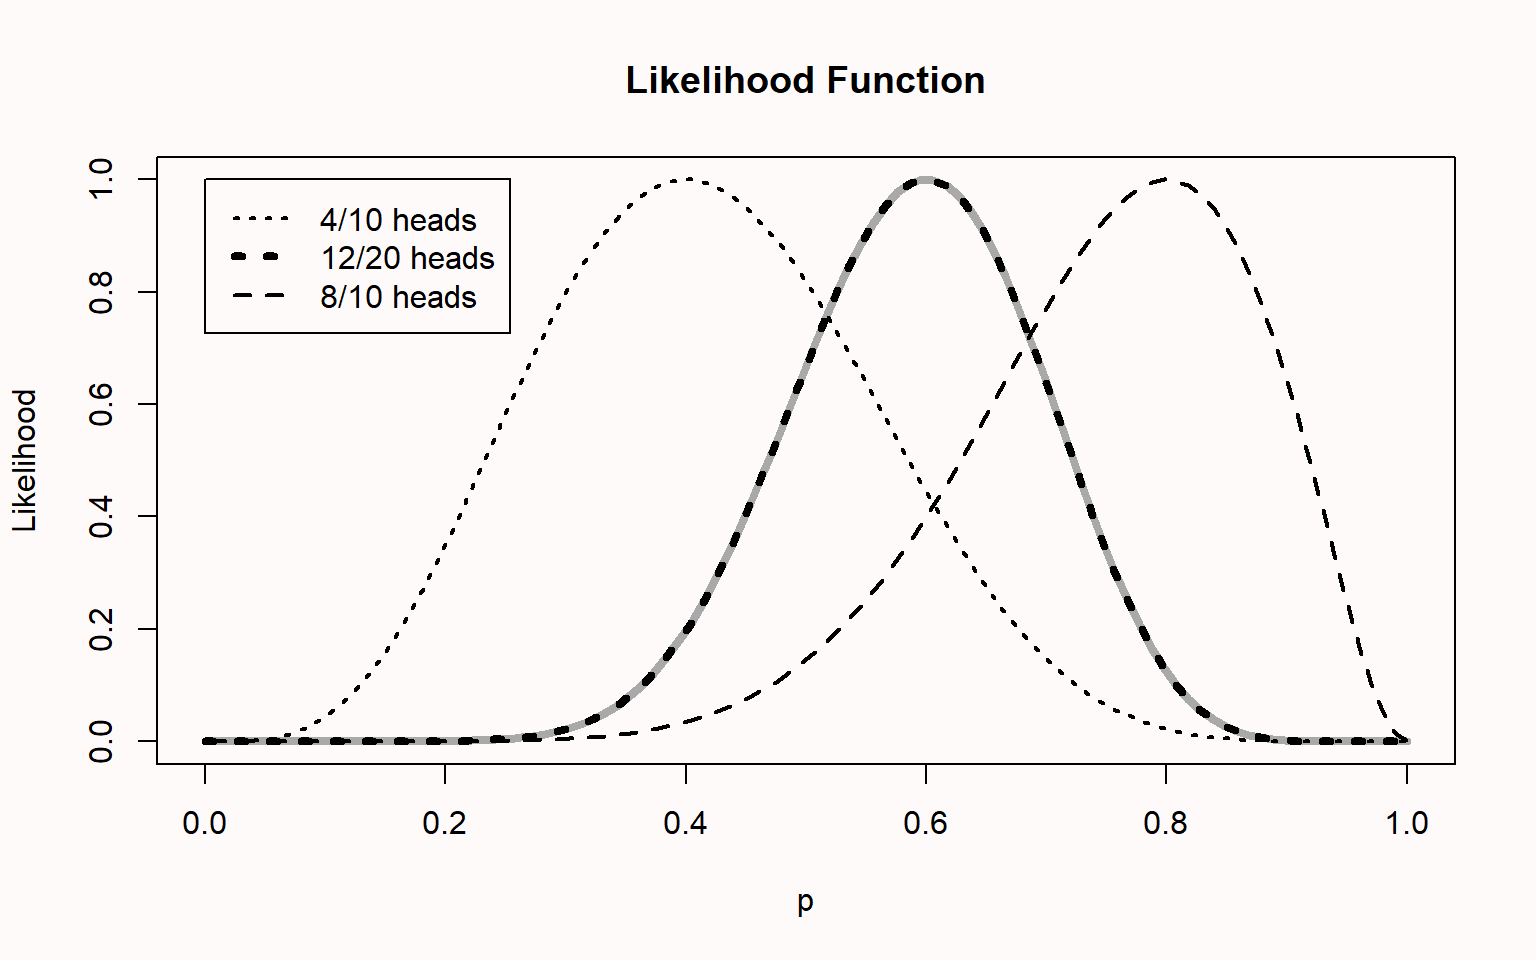
\includegraphics[width=1\linewidth]{03-likelihoods_files/figure-latex/like3-1} 

}

\caption{Combining likelihoods.}\label{fig:like3}
\end{figure}

The curve on left is for 4 out of 10 heads, the one on the right is for 8 out of 10 heads. The black dotted curve in the middle is for 12 out of 20 heads. The grey curve, exactly underneath the 12 out of 20 heads curve, is calculated by multiplying the likelihood curves: L(p\_combined) \emph{=} L(p = 0.8) * L(p = 0.4).

In Figure \ref{fig:like4} we see likelihood curves for 10, 100, and 1000 coin flips, which yield 5, 50, and 500 heads, respectively. The likelihood curves are again standardized to make them more easily comparable. As the sample size increases, the curves become more narrow (the dashed line is for \emph{n} = 10, the dotted line is for \emph{n} = 100, and the solid line is for \emph{n} = 1000). This means that as the sample size increases, our data become increasingly less likely under population parameters further removed from the observed number of heads. In other words, we have collected increasingly strong evidence for \emph{p} = 0.5, compared to most other possible population parameters.

\begin{figure}

{\centering 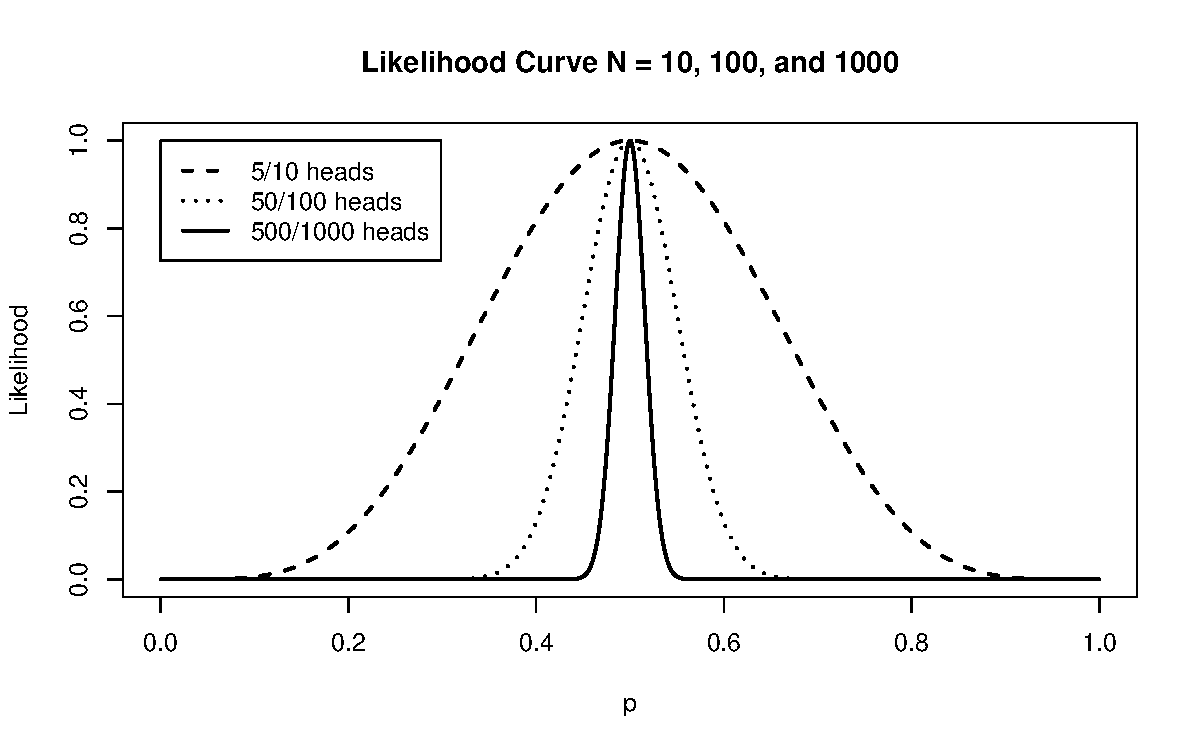
\includegraphics[width=1\linewidth]{03-likelihoods_files/figure-latex/like4-1} 

}

\caption{Likelihood function for 5/10, 50/100 and 500/1000 heads in coin flips.}\label{fig:like4}
\end{figure}

We can use the likelihood function to compare possible values of θ. For example, we might believe the coin we flipped was fair, even though we flipped eight out of ten heads. A fair coin will have \emph{p} = 0.5, while we observed \emph{p} = 0.8. The likelihood function allows us to compute the relative likelihood for different possible parameters. How much more likely is our observed data under the hypothesis that this is an unfair coin that will on average turn up heads 80\% of the time, compared to the alternative theory that this is a fair coin which should turn up heads 50\% of the time?

We can calculate the likelihood ratio:

\[
\frac{L(p = 0.8)}{L(p = 0.5)}
\]

Which is 0.302/0.044 = 6.87. In the plot, both circles show the points on
the likelihood curve for L(\emph{p} = 0.5) and L(\emph{p} = 0.8).

\begin{figure}

{\centering 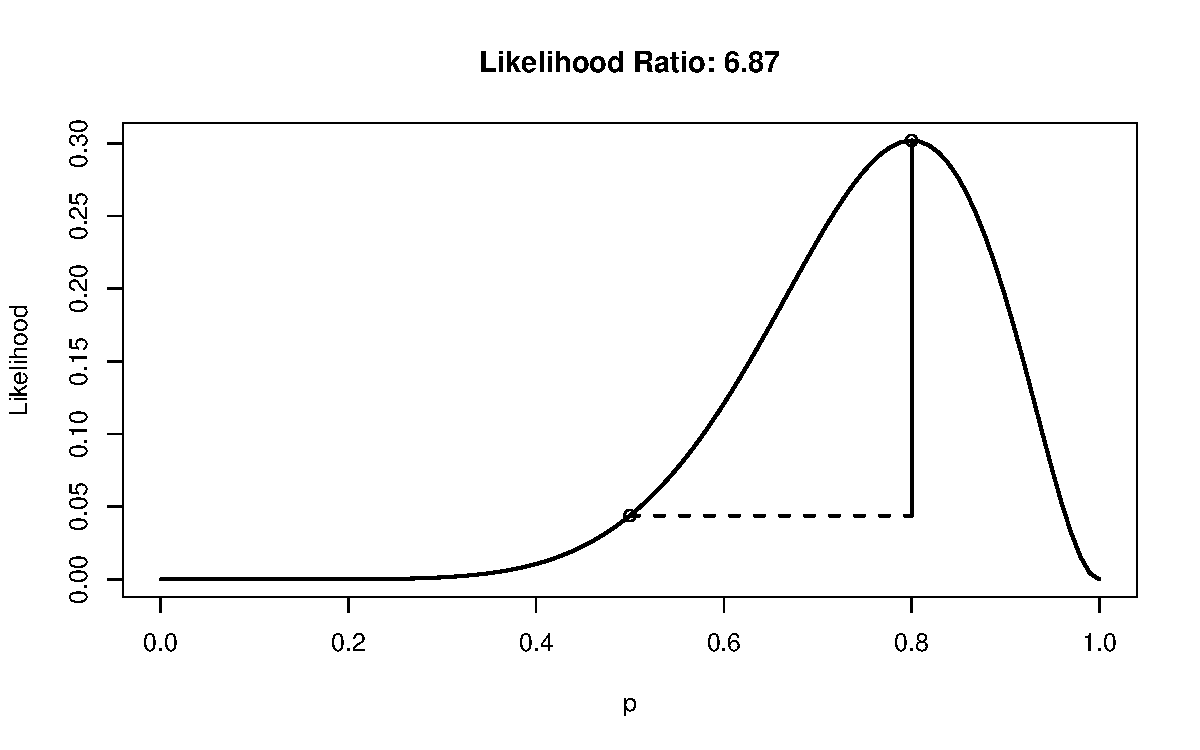
\includegraphics[width=1\linewidth]{03-likelihoods_files/figure-latex/like5-1} 

}

\caption{Computing a likelihood ratio for *p* = 0.5 relative to *p* = 0.8 when observing *p* = 0.8.}\label{fig:like5}
\end{figure}

We can subjectively interpret this likelihood ratio, which tells us an unfair coin that our observed data is 6.87 times more likely under the hypothesis that this coin will turn up heads 80\% of the time, than under the hypothesis that this is a fair coin. How convincing is this? Let's round the likelihood ratio to 7, and imagine two bags of marbles. One bag contains 7 blue marbles. The second contains 7 marbles, each one a different color of the rainbow, so violet, indigo, blue, green, yellow, orange, and red. Someone randomly picks one of the two bags, draws a marble, and shows it to you. The marble is blue: How certain are you this marble came from the bag with all blue marbles, compared to the bag with rainbow coloured marbles? This is how strong the likelihood ratio tells us to believe our data were generated by an unfair coin that turns up heads 80\% of the time, relative to a fair coin, given that we have observed 8 heads in 10 tosses.

Note that likelihood ratios give us the relative evidence for one specified hypothesis, over another specified hypothesis. The likelihood ratio can be calculated for any two hypothesized values. For example, in Figure \ref{fig:like6} below, the likelihood ratio is calculated that compares the hypothesis for a fair coin (\emph{p} = 0.5) with the alternative hypothesis that the coin comes up heads 80\% of the time (\emph{p} = 0.8), when we have observed 4 heads out of 10 coin flips. We see that the observed data are 0.2050/0.0055=37.25 times more likely (ignoring rounding differences -- and try to calculate these numbers by hand using the formula provided earlier) under the hypothesis that this is a fair coin is than under the hypothesis that this is a coin that turns up heads 80\% of the time.

\begin{figure}

{\centering 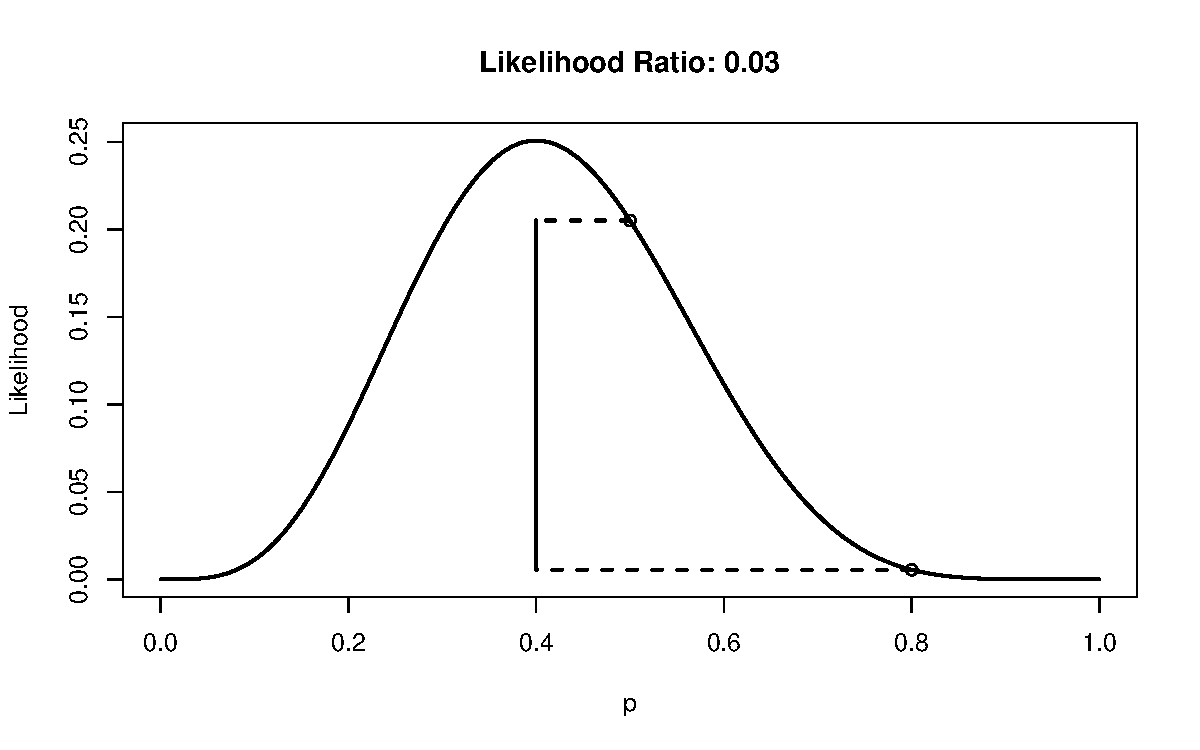
\includegraphics[width=1\linewidth]{03-likelihoods_files/figure-latex/like6-1} 

}

\caption{Computing a likelihood ratio for *p* = 0.5 relative to *p* = 0.8 when observing *p* = 0.4.}\label{fig:like6}
\end{figure}

A likelihood ratio of 1 means the data are equally likely under both hypotheses. Values further away from 1 indicate that the data are more likely under one hypothesis than the other. The ratio can be expressed in favor of one hypothesis over the other (for example L(\emph{p} = 0.5)/L(\emph{p} = 0.8) or vice versa (L(\emph{p} = 0.8)/L(\emph{p} = 0.5). This means the likelihood ratio of 37.25 for H0 relative to H1 is equivalent to a likelihood ratio of 1/37.25 = 0.02685 for H1 relative to H0. Likelihood ratios range from 0 to infinity, and the closer to zero or infinity, the stronger the relative evidence for one hypothesis over the other. We will see in the chapter on \protect\hyperlink{bayes}{Bayesian statistics} that likelihood ratios are in this sense very similar (and a special case of) a Bayes Factor.

Likelihoods are relative evidence. Just because the data are more likely under one possible value of \emph{p} than another value of \emph{p} doesn't mean that the data have come from either of these two distributions. Other values might generate even higher likelihood values. For example, consider the situation where we flip a coin 100 times, and observe 50 heads. We compare \emph{p} = 0.3 versus \emph{p} = 0.8, and find that the likelihood ratio is 803462, implying that there is 803461 times more evidence in the data for \emph{p} = 0.3 than for \emph{p} = 0.8. That might sound pretty conclusive evidence for \emph{p} = 0.3. But it is only relative evidence for \emph{p} = 0.3 compared to \emph{p} = 0.8. If we look at the likelihood function, we clearly see that, not surprisingly, \emph{p} = 0.5 is the value that maximizes the likelihood function. Just because one hypothesis is more likely than another hypothesis, does not mean that there isn't a third hypothesis that is even more likely.

\begin{figure}

{\centering 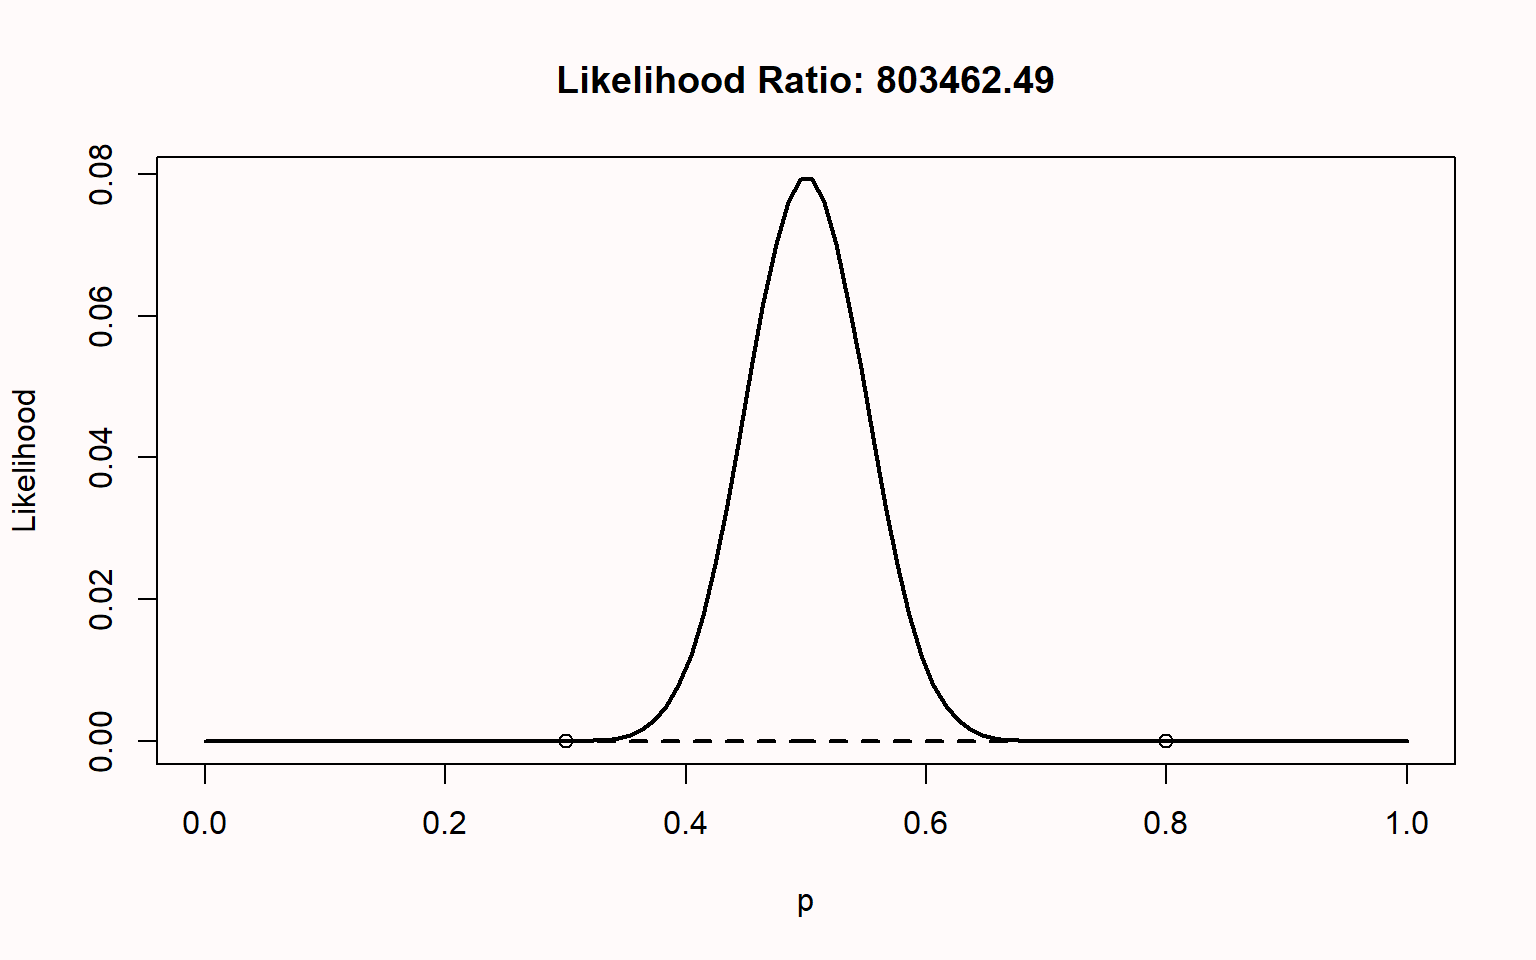
\includegraphics[width=1\linewidth]{03-likelihoods_files/figure-latex/like7-1} 

}

\caption{Computing a likelihood ratio for *p* = 0.3 relative to *p* = 0.8 when observing *p* = 0.5 in 100 coin flips.}\label{fig:like7}
\end{figure}

\hypertarget{likelihood-of-mixed-results-in-sets-of-studies}{%
\section{Likelihood of mixed results in sets of studies}\label{likelihood-of-mixed-results-in-sets-of-studies}}

Science is a cumulative process, and we should evaluate lines of research, not single studies. One big problem in the scientific literature is that nonsignificant results are often never published \citep{franco_publication_2014, fanelli_positive_2010}. At the same time, because the statistical power of hypothesis tests are never 100\% (and often much lower), it is a mathematical reality that it is unlikely (or ``too good to be true'') that a set of multiple studies yields exclusively significant results. \citep{schimmack_ironic_2012, francis_frequency_2014}. We can use binomial likelihoods to examine how likely it is to observe mixed results, and understand when mixed results are nevertheless strong evidence for the presence of an effect. The following is largely based on \citet{lakens_too_2017}.

The probability of observing a significant or nonsignificant result in a study depends on the Type 1 error rate (\(\alpha\)), the statistical power of the test (1-\(\beta\)), and the probability that the null hypothesis is true \citep{wacholder_assessing_2004}. There are four possible outcomes of a study: a true positive, a false positive, a true negative, and a false negative. When H0 is true, the probability of observing a false positive depends on the \(\alpha\) level or the Type 1 error rate (e.g., 5\%). When H1 is true, the probability of observing a true positive depends on the statistical power of the performed test (where an often recommended minimum is 80\%), which in turn depends on the \(\alpha\) level, the true effect size, and the sample size. With an \(\alpha\) level of 5\%, and when H0 is true, a false positive will occur with a 5\% probability (as long as error rates are controlled, e.g., in preregistered studies) and true negative will occur with a 95\% probability. When a test has 80\% power, and H1 is true, a true positive has a probability of 80\%, and a false negative has a probability of 20\%.

If we perform multiple studies, we can calculate the binomial probability that we will observe a specific number of significant and nonsignificant findings \citep{ioannidis_exploratory_2007}. We can calculate the probability of finding exactly two significant results out of three studies assuming the null hypothesis is true. When H0 is true, the probability of significant results equals the \(\alpha\) level, and thus when the \(\alpha\) level is carefully controlled (e.g., in preregistered studies) \emph{p} = 0.05. When k = 2, n = 3, and \emph{p} = .05, the binomial probability function tells us that the probability of finding exactly two significant results in three studies is 0.007 (0.05 × 0.05 × 0.95 = 0.002375, and there are three orders in which two of the three results can be observed, so 0.002375 × 3 = 0.007).

To calculate the likelihood assuming H1 is true, we need to make an assumption about the power in each study. Let's provisionally assume all studies were powered at 80\% and thus \emph{p} = .80. The probability of observing exactly two significant results in three studies, assuming a power of 0.8, is 0.384 (0.8 × 0.8 × 0.2 = 0.128, and with three orders in which two of the three results can be significant, 0.128 × 3 = 0.384). In other words, if you set out to perform 3 studies, your hypothesis is correct, and you test your hypothesis with 80\% power, there is a 38.4\% probability of observing 2 out of 3 significant results, and a 9.6\% probability to observe 1 out of 3 significant results (and for an extremely unlucky individual, a 0.8\% probability of not finding any significant results in three studies, even though there is a true effect). Unless power is extremely high, mixed results should be expected in sets of studies.

Both likelihoods at \emph{p} = .05 and \emph{p} = .80 are highlighted in Figure \ref{fig:like8} by the circles on the dotted vertical lines.We can use the likelihood of the data assuming H0 or H1 is true to calculate the likelihood ratio, 0.384/0.007 = 53.89, which tells us the observed outcome of exactly two significant results out of three studies is 53.89 times more likely when H1 is true and studies had 80\% power, than when H0 is true and studies a carefully controlled 5\% Type 1 error rate. Likelihood ratios of 8 and 32 have been proposed as benchmarks of moderately strong and strong evidence, respectively \citep{royall_statistical_1997}, which implies that finding two significant results out of the three studies could be considered strong evidence for H1, assuming 80\% power. A Shiny app to perform these calculations is available \href{https://shiny.ieis.tue.nl/mixed_results_likelihood/}{here}.

\textbackslash begin\{figure\}

\{\centering 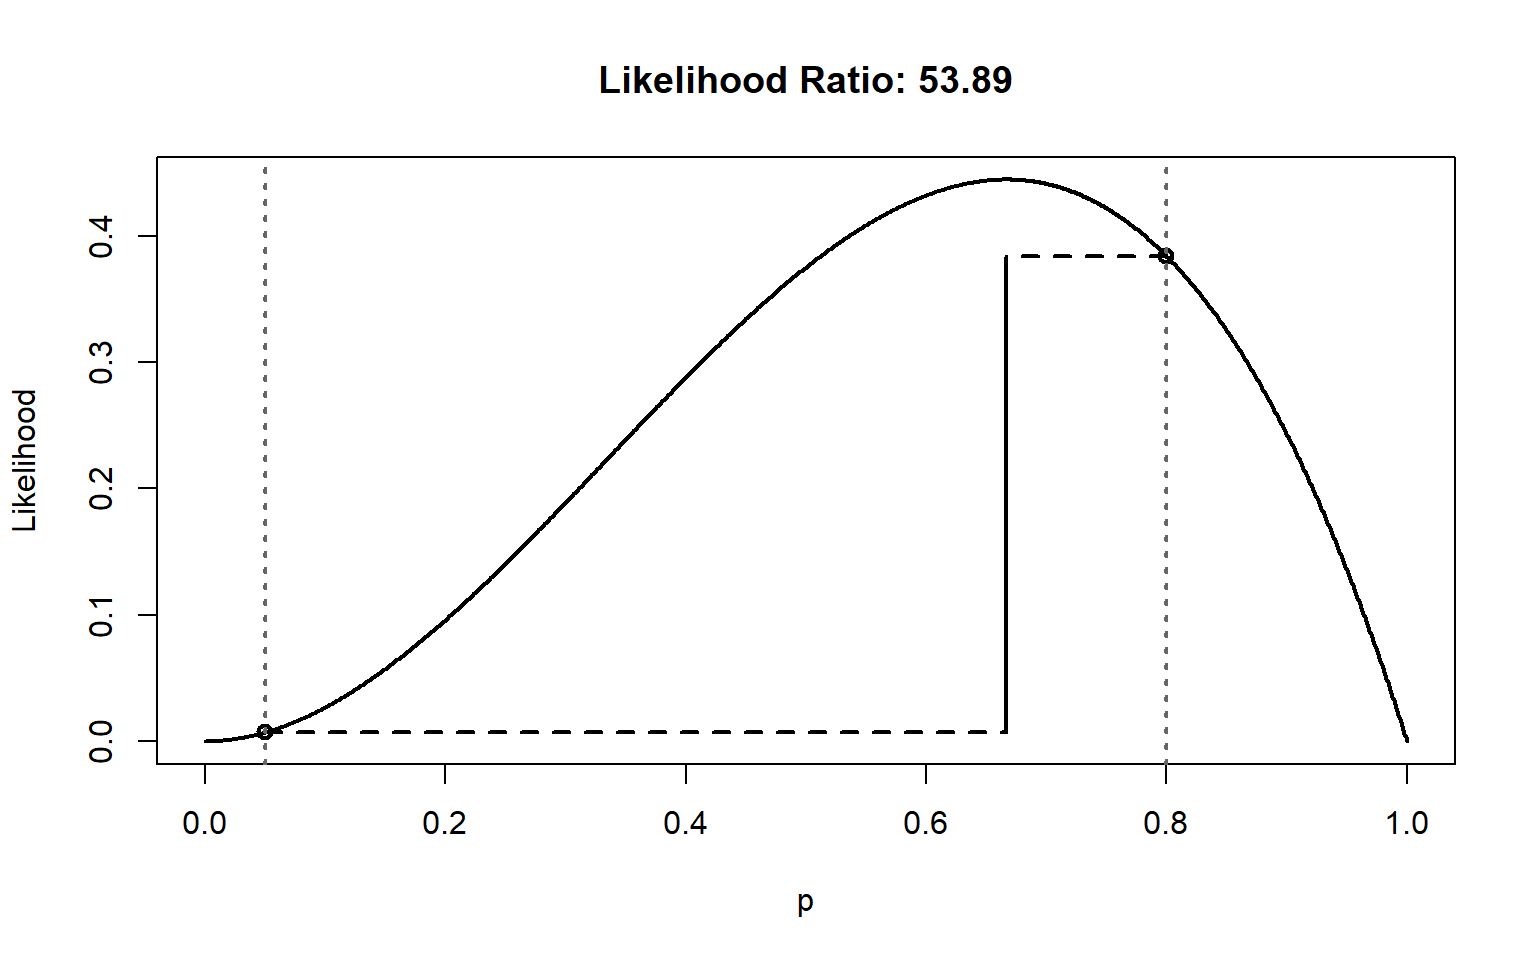
\includegraphics[width=1\linewidth]{03-likelihoods_files/figure-latex/like8-1}

\}

\textbackslash caption\{Computing a likelihood ratio for 2 out of three significant results, assuming an alpha of 5\% and 80\% power.\}\label{fig:like8}
\textbackslash end\{figure\}

In sets of studies, the likelihood ratio in favor of H1 versus H0 after observing a mix of significant and nonsignificant findings can become surprisingly large. Even though the evidence appears to be mixed, there is actually strong evidence in favor of a true effect. For example, when a researcher performs six studies with 80\% power and a 5\% a level and finds three significant outcomes and three nonsignificant outcomes, the cumulative likelihood ratio is convincingly large at 38-to-1 in favor of H1 to consider the set of studies strong evidence for a true effect. Intuitively, researchers
might not feel convinced by a set of studies where three out of six results were statistically significant. But if we do the math, we see that such a set of studies can be very strong evidence in favor of a true effect. A better understanding of these probabilities might be an important step in mitigating the negative effects of publication bias.

Hopefully, researchers become more inclined to submit nonsignificant findings for publication when they have a better understanding of the evidential value in lines of research with mixed results. Publishing all performed studies in lines of research will reduce publication bias, and increase the informational value of the data in the scientific literature. Expecting all studies in lines of research to be statistically significant is not reasonable, and it is important that researchers develop more realistic expectations if they are to draw meaningful inferences from lines of research. We don't have a very good feeling for what real patterns of studies look like, because we are continuously exposed to a scientific literature that does not reflect reality. Almost all multiple study papers in the scientific literature present only statistically significant results, even though this is unlikely given the power of these studies, and the probability that we would only study correct predictions \citep{scheel_excess_2021}. Educating researchers about binomial probabilities and likelihood ratios is a straightforward way to develop more realistic expectations about what research lines that contain evidential value in favor of H1 actually look like.

\hypertarget{likettest}{%
\section{\texorpdfstring{Likelihoods for \emph{t}-tests}{Likelihoods for t-tests}}\label{likettest}}

So far we have computed likelihoods for binomial probabilities, but likelihoods can be computed for any statistical model \citep{glover_likelihood_2004, pawitan_all_2001}. For example, we can compute the relative likelihood of observing a \emph{t}-value under the null and an alternative hypothesis (Figure \ref{fig:like9}). Of course, the observed data is most likely if we assume the observed effect equals the true effect, but examining the likelihood reveals that there are many alternative hypotheses that are relatively more likely than the null hypothesis. This also holds when observing nonsignificant results, which can be more likely under an alternative hypothesis of interest, than under the null hypothesis. This is a reason why it is incorrect to say that there is no effect when \emph{p} \textgreater{} \(\alpha\) (see \protect\hyperlink{misconception1}{\emph{p}-value misconception 1}).

\begin{figure}

{\centering 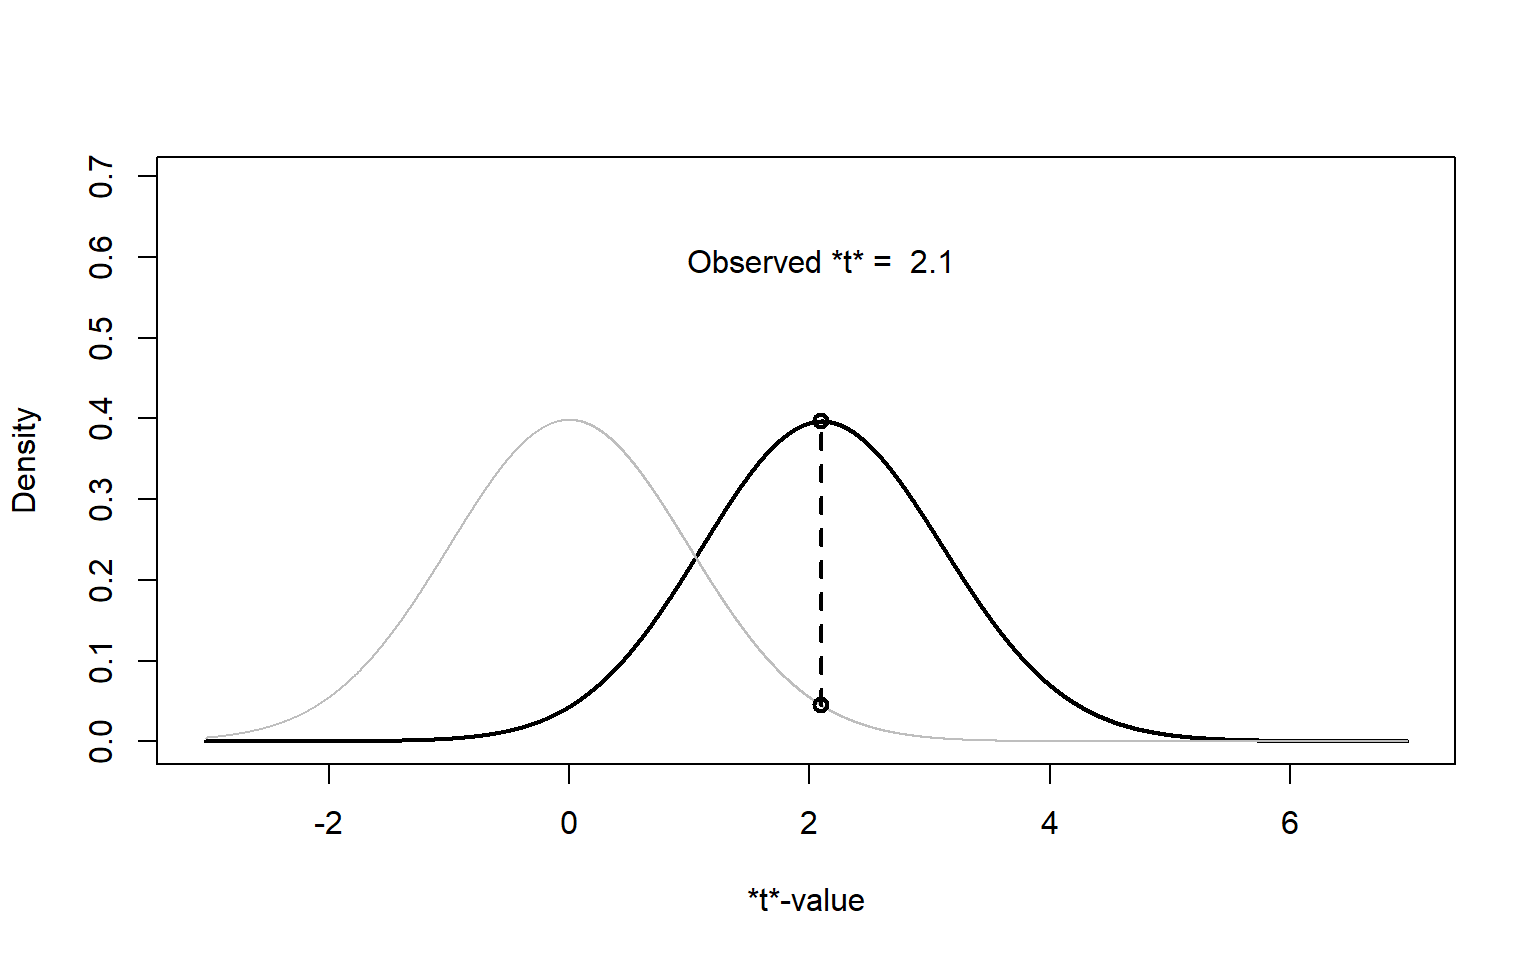
\includegraphics[width=1\linewidth]{03-likelihoods_files/figure-latex/like9-1} 

}

\caption{Likelihood ratio for observed *t*-value under H0 and H1.}\label{fig:like9}
\end{figure}

\hypertarget{test-yourself-2}{%
\section{Test Yourself}\label{test-yourself-2}}

\textbf{Q1:} Which statement is correct when you perform 3 studies?

\begin{enumerate}
\def\labelenumi{\Alph{enumi})}
\tightlist
\item
  When H1 is true, alpha = 0.05, and power = 0.80, it is almost as likely to observe one or more non-significant results (48.8\%) as it is to observe only significant results (51.2\%).
\item
  When alpha = 0.05 and power = 0.80, it is extremely rare that you will find 3 significant results (0.0125\%), regardless of whether H0 is true or H1 is true.
\item
  When alpha = 0.05 and power = 0.80, 2 out of 3 statistically significant results is the most likely outcome overall (38.4\%) when H1 is true.
\item
  When alpha = 0.05 and power = 0.80, the probability of finding at least one false positive (a significant result when H0 is true) in three studies is 5\%.
\end{enumerate}

\textbf{Q2:} Sometimes in lines of three studies, you'll find a significant effect in one study, but there is no effect in the other two related studies. Assume the two related studies were not exactly the same in every way (e.g., you have changed the manipulation, or the procedure, or some of the questions). It could be that the two other studies did not work because of minor differences that had some effect you do not fully understand yet. Or it could be that the single significant result was a Type 1 error, and H0 was true in all three studies. Which statement below is correct, assuming a 5\% Type 1 error rate and 80\% power?

\begin{enumerate}
\def\labelenumi{\Alph{enumi})}
\tightlist
\item
  All else being equal, the probability of a Type 1 error in one of three studies is 5\% when there is no true effect in all three studies, and the probability of finding exactly 1 in three significant effects, assuming 80\% power in all three studies, is 80\%, which is substantially more likely.
\item
  All else being equal, the probability of a Type 1 error in one of three studies is 13.5\% when there is no true effect in all three studies, and the probability of finding exactly 1 in three significant effects, assuming 80\% power in all three studies (and thus a true effect), is 9.6\%, which is slightly, but not substantially less likely.
\item
  All else being equal, the probability of a Type 1 error in one of three studies is 85.7\% when there is no true effect in all three studies, and the probability of finding exactly 1 in three significant effects, assuming 80\% power in all three studies (and thus a true effect) (and thus a true effect), is 0.8\%, which is substantially less likely.
\item
  It is not possible to know the probability you will observe a Type 1 error if you perform 3 studies.
\end{enumerate}

The idea that most studies have 80\% power is slightly optimistic. \textbf{Examine the correct answer to the previous question across a range of power values} (e.g., 50\% power, and 30\% power).

\textbf{Q3:} Several papers suggest it is a reasonable assumption that the power in the psychological literature might be around 50\%. Set the number of studies to 4, the number of successes also to 4, and the assumed power slider to 50\%, and look at the table at the bottom of the app. How likely is it to observe 4 significant results in 4 studies, assuming there is a true effect?

\begin{enumerate}
\def\labelenumi{\Alph{enumi})}
\tightlist
\item
  6.25\%
\item
  12.5\%
\item
  25\%
\item
  37.5\%
\end{enumerate}

Imagine you perform 4 studies, and 3 show a significant result. \textbf{Change these numbers in the online app. Leave the power at 50\%}. The output in the text tells you:

\emph{When the observed results are equally likely under H0 and H1, the likelihood ratio is 1. Benchmarks to interpret Likelihood Ratios suggest that when 1\textless LR\textless8 there is weak evidence, when 8\textless LR\textless32 there is moderate evidence, and when LR\textgreater32, there is strong evidence.}

\emph{The data are more likely under the alternative hypothesis than the null hypothesis with a likelihood ratio of 526.32}

These calculations show that, assuming you have observed three significant results out of four studies, and assuming each study had 50\% power, it is 526 times more likely to have observed these data when the alternative hypothesis is true, than when the null hypothesis is true. In other words, it is 526 times more likely to find a significant effect in three studies when you have 50\% power, than to find three Type 1 errors in a set of four studies.

\textbf{Q4}: Maybe you don't think 50\% power is a reasonable assumption. How low can the power be (rounded to 2 digits), for the likelihood to remain higher than 32 in favor of H1 when observing 3 out of 4 significant results?

\begin{enumerate}
\def\labelenumi{\Alph{enumi})}
\tightlist
\item
  5\% power
\item
  17\% power
\item
  34\% power
\item
  44\% power
\end{enumerate}

The main take home message of these calculations is to understand that 1) mixed results are supposed to happen, and 2) mixed results can contain strong evidence for a true effect, across a wide range of plausible power values. The app also tells you how much evidence, in a rough dichotomous way, you can expect. This is useful for our educational goal. But when you want to evaluate results from multiple studies, the formal way to do so is by performing a meta-analysis.

The above calculations make a very important assumption: The Type 1 error rate is controlled at 5\%. If you try out many different tests in each study, and only report the result that yielded a p \textless{} 0.05, these calculations no longer hold.

\textbf{Q5}: Go back to the default settings of 2 out of 3 significant results, but now set the Type 1 error rate to 20\%, to reflect a modest amount of p-hacking. Under these circumstances, what is the \textbf{highest} likelihood in favor of H1 you can get if you explore all possible values for the true power?

\begin{enumerate}
\def\labelenumi{\Alph{enumi})}
\tightlist
\item
  Approximately 1
\item
  Approximately 4.63
\item
  Approximately 6.70
\item
  Approximately 62.37
\end{enumerate}

As the scenario above shows, \emph{p}-hacking makes studies extremely uninformative.
\textbf{If you inflate the error rate, you quickly destroy the evidence in the data.} You can no longer determine whether the data is more likely when there is no effect, than when there is an effect. Sometimes researchers complain that people who worry about \emph{p}-hacking and try to promote better Type 1 error control are missing the point, and that other things (better measurement, better theory, etc.) are more important. I fully agree that these aspects of scientific research are at least as important as better error control. But better measures and theories will require decades of work. Better error control can be accomplished today, if researchers would stop inflating their error rates by flexibly analyzing their data. And as this assignment shows, inflated rates of false positives very quickly make it difficult to learn what is true from the data we collect. Because of the relative ease with which this part of scientific research can be improved, and because we can achieve this today (and not in a decade) I think it is worth stressing the importance of error control, and publish more realistic looking sets of studies.

\textbf{Q6}: Some `prestigious' journals (which, when examined in terms of scientific quality such as reproducibility, reporting standards, and policies concerning data and material sharing, are quite low quality despite their prestige) only publish manuscripts with a large number of studies, which should all be statistically significant. If we assume an average power in psychology of 50\%, only 3.125\% of 5 study articles should contain exclusively significant results. If you pick up a random issue from such a prestigious journal, and see 10 articles, each reporting 5 studies, and all manuscripts have exclusively significant results, would you trust the reported findings more, or less, than when all these articles had reported mixed results? Why?

\textbf{Q7}: Unless you will power all your studies at 99.99\% for the rest of your career (which would be slightly inefficient, but great if you don't like insecurity), you will observe mixed results in lines of research. How do you plan to deal with mixed results in lines of research?

\hypertarget{bayes}{%
\chapter{Bayesian statistics}\label{bayes}}

\begin{quote}
``Logic!'' said the Professor half to himself. ``Why don't they teach logic at these schools? There are only three possibilities. Either your sister is telling lies, or she is mad, or she is telling the truth. You know she doesn't tell lies and it is obvious that she is not mad. For the moment then and unless any further evidence turns up, we must assume that she is telling the truth.''
\end{quote}

\emph{\href{https://gutenberg.ca/ebooks/lewiscs-thelionthewitchandthewardrobe/lewiscs-thelionthewitchandthewardrobe-00-h.html}{The Lion, The Witch, and The Wardrobe. A Story for Children} by C. S. Lewis.}

In the children's book The Lion, The Witch, and The Wardrobe, both Lucy and Edmund go through a wardrobe into a country called Narnia. Lucy tells their older brother and sister, Peter and Susan, about Narnia, but Edmund wants to keep it a secret, and tells Peter and Susan they were just pretending. Peter and Susan don't know what to believe - does Narnia exist, or not? They ask the Professor, who lives in the house with the wardrobe, for advice. The Professor asks Susan and Peter if in their past experience, Lucy or Edward has been more truthful, to which Peter answers ``Up till now, I'd have said Lucy every time.'' The Professor then replies with the quote above. From the three possible options, it is very unlikely that Lucy is lying, as she has not done this in the past, and the Professor says it is clear just from talking to Lucy that she is not mad. Therefore, the most likely option is that Lucy is telling the truth. If new evidence is uncovered, these beliefs can be updated in the future. This approach to knowledge generation, where the prior probability of different hypotheses is quantified, and if possible updated in light of new data, is an example of \emph{Bayesian inference}.

Although frequentist statistics is by far the dominant approach in science, it is important to have had at least rudimentary exposure to Bayesian statistics during any statistics training. Bayesian statistics is especially useful when inferences are made in cases where the data under investigation is unique, and there is no frequentist probability defined as the limit in many trials. For example, the question might not be how often Lucy lies on average, but whether Lucy is lying in this specific instance about the existence of Narnia. When we do research, we often start with a prior belief that a hypothesis is true. After collecting data, we can use this data to update our prior beliefs. Bayesian statistics allows you to update prior beliefs into posterior probabilities in a logically consistent manner. Before we have collected data, the \textbf{prior odds} of Hypothesis 1 (H1) over the null-hypothesis (H0) are P(H1)/P(H0), After we have collected data, we have the \textbf{posterior odds} P(H1\textbar D)/P(H0\textbar D), which you can read as the probability of H1, given the data, divided by the probability of H0, given the data. There are different approaches to Bayesian statistics. We will first discuss Bayes factors, and then Bayesian estimation.

\hypertarget{bayes-factors}{%
\section{Bayes factors}\label{bayes-factors}}

One approach in Bayesian statistics focuses on the comparison of different models that might explain the data (referred to as \textbf{model comparison}). In Bayesian statistics, the probability of data under a specified model (D\textbar P(H0) is a number that expressed what is sometimes referred to as the absolute \textbf{evidence}, and more formally referred to as a marginal likelihood. The marginal likelihood uses prior probabilities to average the likelihood across the parameter space. For example, assume we have a simple model \emph{M} that is
based on a single parameter, that can take on two values, X and Y, and that a-prior we believe the probability of both values is p(X) = 0.4 and p(Y) = 0.6. We collect data, and calculate the likelihood for both these parameter values, which is p(D\textbar X) = 0.02 and p(D\textbar Y) = 0.08. The marginal likelihood of our model \emph{M} is then P(D\textbar M) = 0.4 × 0.02 + 0.6 × 0.08 = 0.056. Most often, models have continuously varying parameters, and the marginal likelihood formula is based on an integral, but the idea remains the same.

A comparison of two models is based on the relative evidence the data provides for each models we are comparing. The relative evidence is calculated by dividing the marginal likelihood for one model by the marginal likelihood for another model, and this ratio of relative evidence based on these marginal likelihoods is called the \textbf{Bayes factor}. Bayes factors are the Bayesian equivalent of hypothesis tests \citep{dienes_understanding_2008}. The Bayes factor represents how much we have updated our beliefs, based on observing the data. We can express Bayes factors to indicate how much more likely H1 is given the data compared to H0 (often indicated by B10) or as how much more likely H0 has become compared to H1 (B01), and B10 = 1/B01. Similar to likelihood ratios of 1, a Bayes factor of 1 did not change our beliefs for one model compared to the other model. A very large Bayes factor for H1 over H0 has increased our belief in H1, and a Bayes Factor close for H1 over H0 to 0 has increased our belief in H0. If our prior belief in H1 was very, very low (e.g., your belief in unicorns) even a large Bayes factor that supports the presence of a unicorn might not yet convince you that unicorns are real -- but you have updated your belief in unicorns, and now believe they are at least more likely then they were before (even if you still think unicorns are very unlikely to exist). The contribution of the Bayes Factor and the prior in calculating the posterior odds is clear in the following formula:

\[
\frac{P(H1|D)}{P(H0|D)} = \ \frac{P(D|H1)}{P(D|H0)}\  \times \ \frac{P(H1)}{P(H0)}
\]

\[
Posterior\ Probability = \ Bayes\ Factor\  \times \ Prior\ Probability
\]

A Bayesian analysis of data requires specifying the prior. Here, we will continue our example based on a binomial probability, such as a coin flip. In the likelihood example, we compared two point hypotheses (e.g., \emph{p} = 0.5 vs.~\emph{p} = 0.8). In Bayesian statistics, parameters are considered to be random variables, and the uncertainty or degree of belief with respect to the parameters is quantified by \textbf{probability distributions}.

A binomial probability lies between 0 and 1. You could draw any probability density you want over 0 and 1, and turn it into a prior, but for good reasons (simplicity, mostly) a beta-prior is often used for binomial probabilities. The shape of the beta-prior depends on two parameters, \(\alpha\) and \(\beta\). Note that these are the same Greek letters as used for the Type 1 error rate and Type 2 error rate, but that is purely coincidental! The \(\alpha\) and \(\beta\) in binomial probabilities are unrelated to error rates, and the use of the same letters is mainly due to a
lack of creativity among statisticians and the limited choice the alphabet gives us. It also does not help that \(\beta\) is one of the parameters of the Beta distribution. Try to keep these different Beta's apart! The probability density function is:

\[
\int_{}^{}{\left( x,\ \alpha,\ \beta \right) = \ \frac{1}{B(\alpha,\beta)}}x^{\alpha - 1}{(1 - x)}^{\beta - 1}
\]

where \emph{B(\(\alpha\), \(\beta\))} is the beta function. Understanding the mathematical basis of this function is beyond the scope of this chapter, but you can read more on \href{https://en.wikipedia.org/wiki/Beta_distribution}{Wikipedia} or Kruschke's book on Doing Bayesian Data Analysis \citep{kruschke_doing_2014}. The beta-prior for a variety of values for \(\alpha\) and \(\beta\) can be seen in the figure below.

\begin{figure}

{\centering 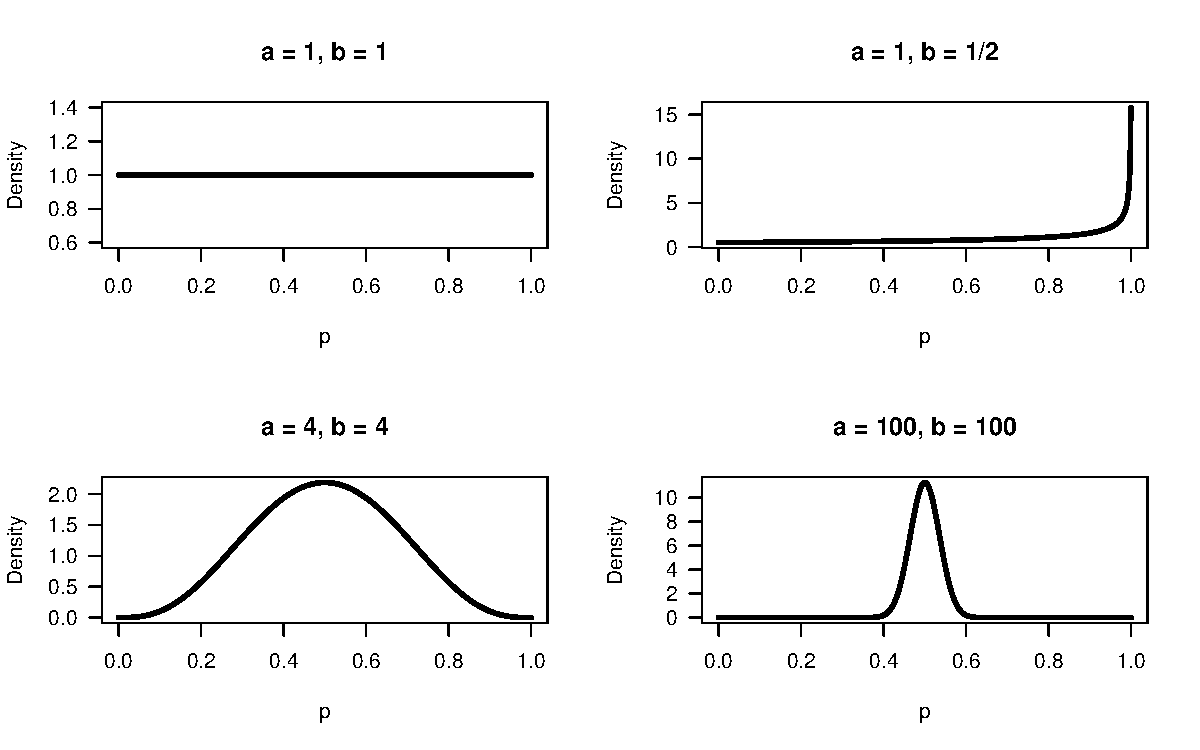
\includegraphics[width=1\linewidth]{04-bayes_files/figure-latex/bayes1-1} 

}

\caption{Four examples of Bayesian priors}\label{fig:bayes1}
\end{figure}

These beta densities reflect different types of priors. Let's assume you are approached by a street merchant who tries to sell you a special coin with heads and tails that, when flipped, will almost always turn up heads. The \(\alpha\) = 1, \(\beta\) = 1 prior is what a newborn baby would have as a prior, without any idea of what to expect when you flip a coin, and thus every value of \emph{p} is equally likely. The \(\alpha\) = 1, \(\beta\) = 1/2 prior is what a true believer would have as a prior. The sales merchant tells you the coin will turn up heads almost every time, and thus, you believe it will turn up heads almost every time. The \(\alpha\) = 4, \(\beta\) = 4, and the \(\alpha\) = 100, \(\beta\) = 100 priors are for slightly and extremely skeptical people. With an \(\alpha\) = 4, \(\beta\) = 4 prior, you expect the coin will be fair, but you are willing to believe a wide range of other true values is possible (the curve is centered on 0.5, but the curve is wide, allowing for very high and low values of \emph{p}). With the \(\alpha\) = 100, \(\beta\) = 100 prior you are really convinced coins are fair, and believe there will be only a very slight bias, at most (the curve is again centered on 0.5, and a skeptic believes the \emph{p} will lie between 0.4 and 0.6 -- a much narrower range compared to the slightly skeptic individual).

Let's assume the newborn baby, the true believer, the slightly skeptic and the extreme skeptic all buy the coin, flip it n = 20 times, and observe x = 10 heads. This outcome can be plotted as a binomial distribution with 10 heads out of 20 trials, or as a Beta(11, 11) distribution.

The newborn baby had a prior Beta distribution with \(\alpha\) = 1 and \(\beta\) = 1, which equals a binomial likelihood distribution for 0 heads out of 0 trials. The posterior is a Beta distribution with Beta(\(\alpha\)*, \(\beta\)*), where:

\(\alpha\)* = \(\alpha\) + x = 1 + 10= 11

\(\beta\)* = \(\beta\) + n -- x = 1 + 20 -- 10 = 11

Or calculating these values more directly from the \(\alpha\) and \(\beta\) of the prior and
likelihood:

\(\alpha\)* = \(\alpha\)prior + \(\alpha\)likelihood -- 1 = 1 + 11 - 1= 11

\(\beta\)* = \(\beta\)prior + \(\beta\)likelihood - 1 = 1 + 11 -- 1 = 11

Thus, the posterior distribution for the newborn is a Beta(11,11) distribution. This equals a binomial likelihood function for 10 heads out of 20 trials, or Beta(11,11) distribution. In other words, the posterior distribution is identical to the likelihood function when a uniform prior is used.

Take a look at the Figure below. Given 10 heads out of 20 coin flips, we see the prior distribution of the newborn (the horizontal grey line), the likelihood (the blue dotted line) and the posterior (the black line).

\begin{figure}

{\centering 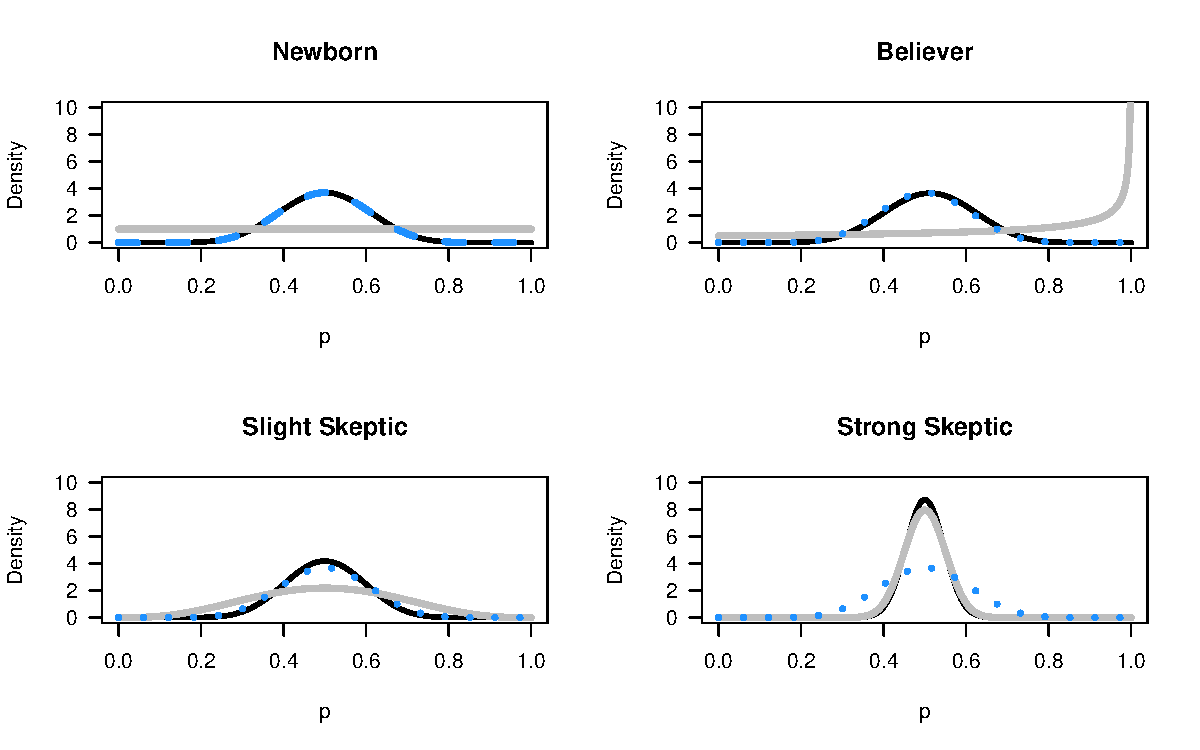
\includegraphics[width=1\linewidth]{04-bayes_files/figure-latex/bayes2-1} 

}

\caption{Four examples of how different priors are updated based on data to the posterior.}\label{fig:bayes2}
\end{figure}

For the true believer the posterior distribution is not centered on the maximum likelihood of the observed data, but just a bit in the direction of the prior. The slightly skeptic and the strong skeptic end up with a much stronger belief in a fair coin after observing the data, but mainly because they already had a stronger prior that the coin was fair.

\hypertarget{updating-our-belief}{%
\section{Updating our belief}\label{updating-our-belief}}

Now that we have a distribution for the prior, and a distribution for the posterior, we can see in the graphs below for which values of \emph{p} our belief has increased. Everywhere where the black line (of the posterior) is higher than the grey line (of the prior) our belief in that \emph{p} has increased.

\begin{figure}

{\centering 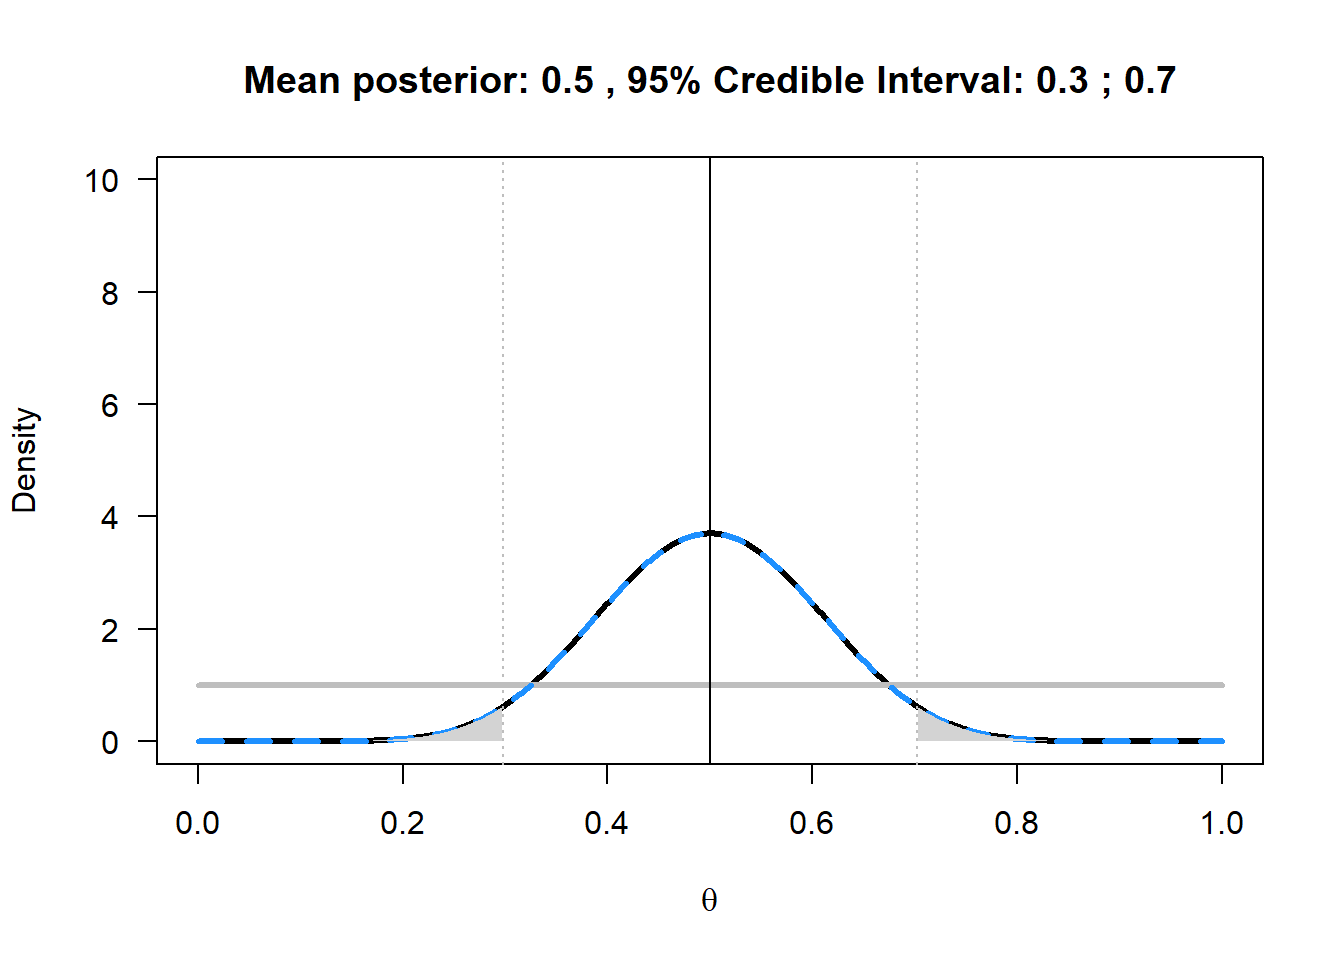
\includegraphics[width=1\linewidth]{04-bayes_files/figure-latex/bayes4-1} 

}

\caption{Plot for the prior, likelihood, and posterior.}\label{fig:bayes4}
\end{figure}

The Bayes Factor is used to quantify this increase in relative evidence. Let's calculate the Bayes Factor for the hypothesis that the coin is fair for the newborn. The Bayes Factor is simply the value of the posterior distribution at \emph{p} = 0.5, divided by the value of the prior distribution at \emph{p} = 0.5:

BF10 = Beta(\emph{p} = 0.5, 11, 11)/Beta(\emph{p} = 0.5, 1, 1) = 3.70/1 = 3.70

You can check this in an \href{http://pcl.missouri.edu/bf-binomial}{online Bayes Factor calculator} by Jeff Rouder and Richard Morey. At successes, fill in 10, at trials, fill in 20. We want to calculate the Bayes Factor for the point null value of \emph{p} = 0.5, so fill in 0.5. The \(\alpha\) and \(\beta\) for the prior are both 1, given the newborns prior of Beta(1,1). Clicking `submit query' will give you the Bayes factor of 3.70.

\begin{figure}

{\centering 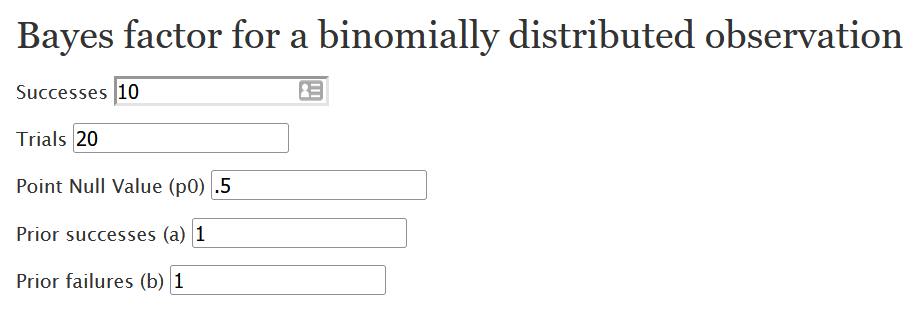
\includegraphics[width=1\linewidth]{images/binombayesonline} 

}

\caption{Screenshot of the online calculator for binomially distributed observations}\label{fig:gpower-screenshot}
\end{figure}

We can calculate and plot the Bayes Factor, and show the prior (grey), likelihood (dashed blue) and posterior (black). For the example of 20 flips, 10 heads, and the newborn prior, the plot looks like this:

\begin{figure}

{\centering 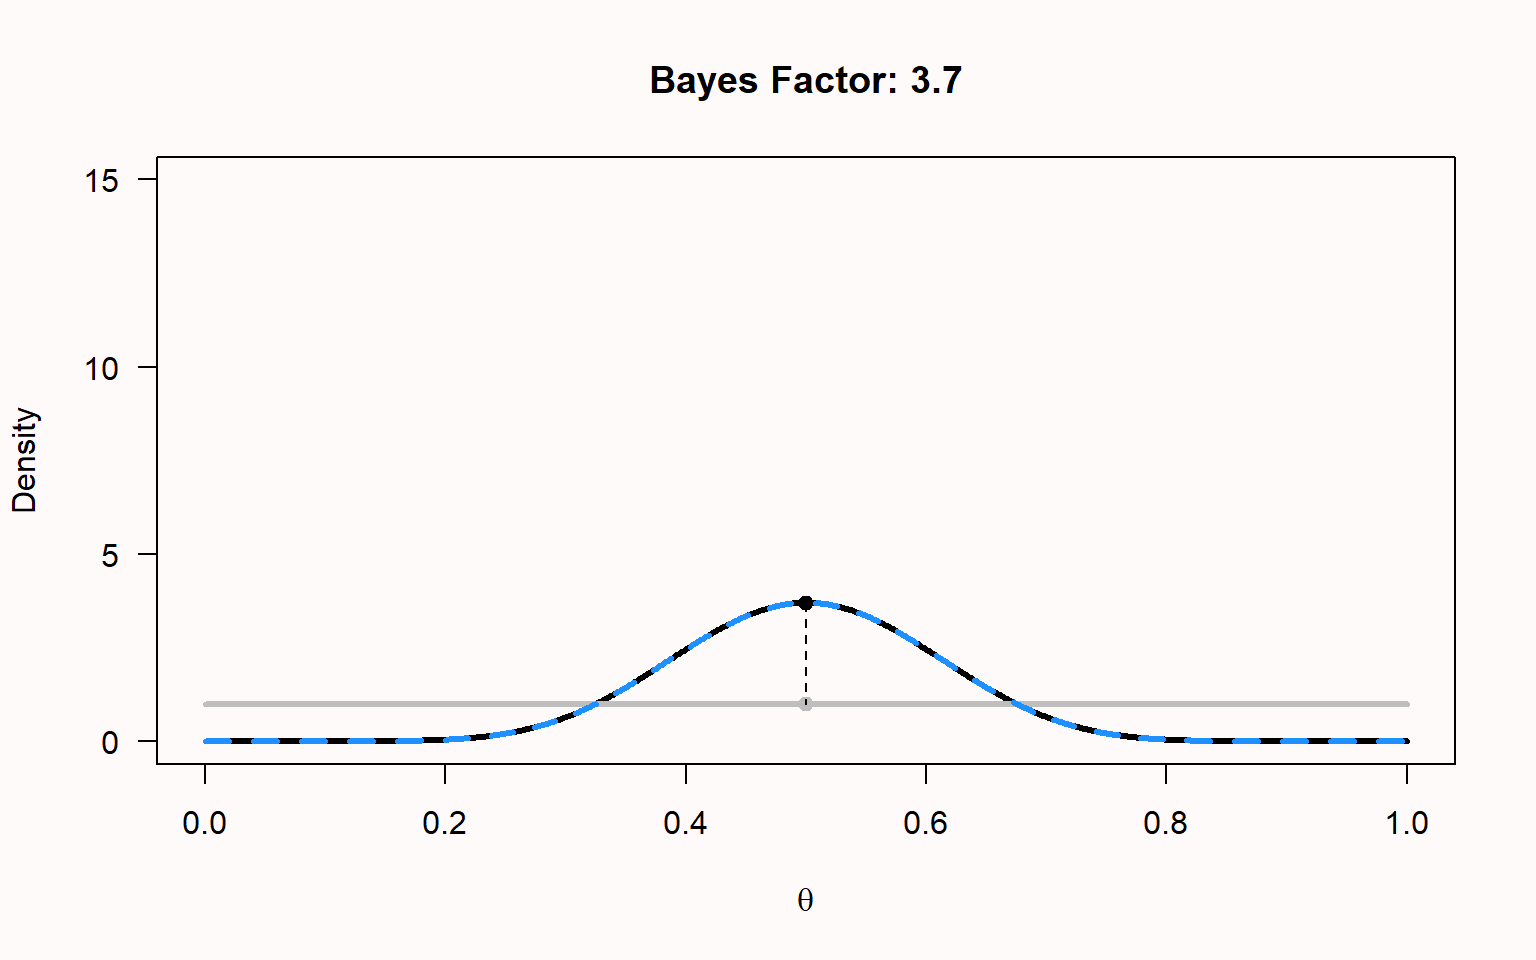
\includegraphics[width=1\linewidth]{04-bayes_files/figure-latex/bayes6-1} 

}

\caption{Plot for the prior, likelihood, and posterior.}\label{fig:bayes6}
\end{figure}

We see that for the newborn, \emph{p} = 0.5 has become more probable, but so has \emph{p} = 0.4. Now let's assume the strong skeptic, who believes the coin is fair with a prior of Beta(100, 100), buys the coin and flips it 100 times. Surprisingly, the coin comes up heads 90 out of 100 flips. The plot of the prior, likelihood, and posterior now looks much more extreme, because we had a very informed prior, and extremely different data. We see the grey prior distribution, the dashed blue likelihood based on the data, and the posterior distribution in black. The Bayes Factor of 0 represents the substantial drop in belief that the coin is fair -- indeed, this now seems an untenable hypothesis, even for the strong skeptic. It shows how data can update your belief. Where a newborn would now completely believe that the true \emph{p} for the coin is somewhere around 0.9, the strong skeptic has more reason to believe the \emph{p} is around 0.65, due to the strong prior conviction that the coin is fair. Given enough data, even this strong skeptic will become convinced that the coin will return heads most of the time as well.

\begin{figure}

{\centering 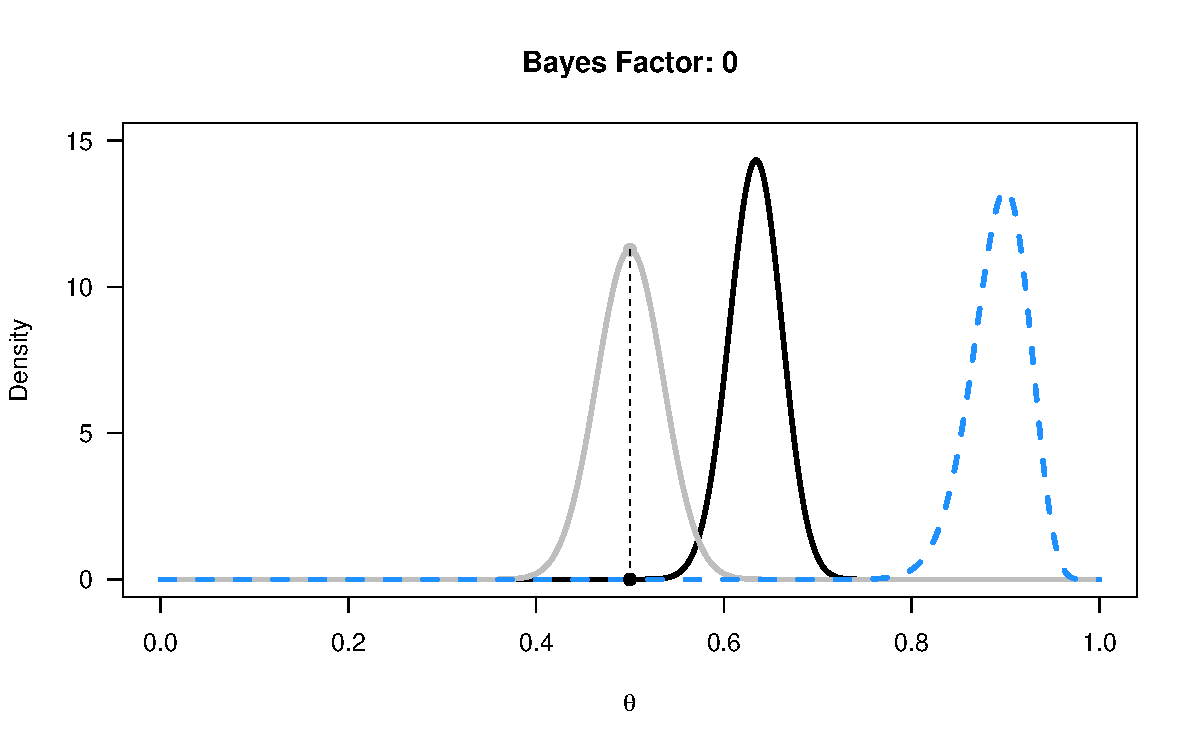
\includegraphics[width=1\linewidth]{04-bayes_files/figure-latex/bayes7-1} 

}

\caption{Plot for the prior, likelihood, and posterior.}\label{fig:bayes7}
\end{figure}

We can now also see the difference between a likelihood inference approach, and a Bayesian inference approach. In likelihood inference, you can compare different values of \emph{p} for the same likelihood curve (e.g., \emph{p} = 0.5 vs \emph{p} = 0.8) and calculate the likelihood ratio. In Bayesian inference, you can compare the difference between the prior and the posterior for the same value of \emph{p}, and calculate the Bayes Factor.

If you have never seen Bayes Factors before, you might find it difficult to interpret the numbers. As with any guideline (e.g., interpreting effect sizes as small, medium, and large) there is criticism on the use of benchmarks. On the other hand, you have to start somewhere in getting a feel for what Bayes Factors mean. A Bayes factor between 1 and 3 is considered `not worth more than a bare mention', larger than 3 (or smaller than 1/3) is considered `substantial', and larger than 10 (or smaller than 1/10) is considered `strong'. These labels refer to the increase in how much you believe a specific hypothesis, not in the posterior belief in that hypothesis. If you think extra-sensory perception is extremely implausible, a single study with a BF = 14 will increase your belief, but you will now think extra-sensory perception is pretty much extremely implausible.

\hypertarget{bayesest}{%
\section{Bayesian Estimation}\label{bayesest}}

The posterior distribution summarizes our belief about the expected number of heads when flipping a coin after seeing the data, by averaging over our prior beliefs and the data (or the likelihood). The mean of a Beta distribution can be calculated by \(\alpha\)/(\(\alpha\)+\(\beta\)). We can thus easily calculate the mean of a posterior distribution, which is the expected value based on our prior beliefs and the data.

We can also calculate a \textbf{credible interval} around the mean, which is a Bayesian version of a confidence interval with a slightly different interpretation. Instead of the Frequentist interpretation where a parameter has one (unknown) true value, the Bayesian approach considers the data fixed, but allow the parameter to vary. In Bayesian approaches, probability distributions represent our degree of belief. When calculating a credible interval, one is saying `I believe it is 95\% probable (given my prior and the data) that the true parameter falls within this credible interval'. A 95\% credible interval is simply the area of the posterior distribution between the 0.025 and 0.975 quantiles.

A credible interval and a confidence interval are the same, when a uniform prior (e.g., Beta(1,1)) is used. In this case, credible interval is numerically identical to the confidence interval. Only the interpretation differs. Whenever an informed prior is used, the credible interval and confidence interval differ. If the chosen prior is not representative of the truth, the credible interval will not be representative of the truth, but it is always a correct formalization of your beliefs. For a single confidence interval, the probability that it contains the true population parameter is either 0 or 1. Only in the long run will 95\% of confidence intervals contain the true population parameter. These are important differences between Bayesian credible intervals and Frequentist confidence intervals to keep in mind.

We can plot the mean for the posterior when 10 heads out of 20 coin flips are observed, given a uniform prior.

\begin{figure}

{\centering 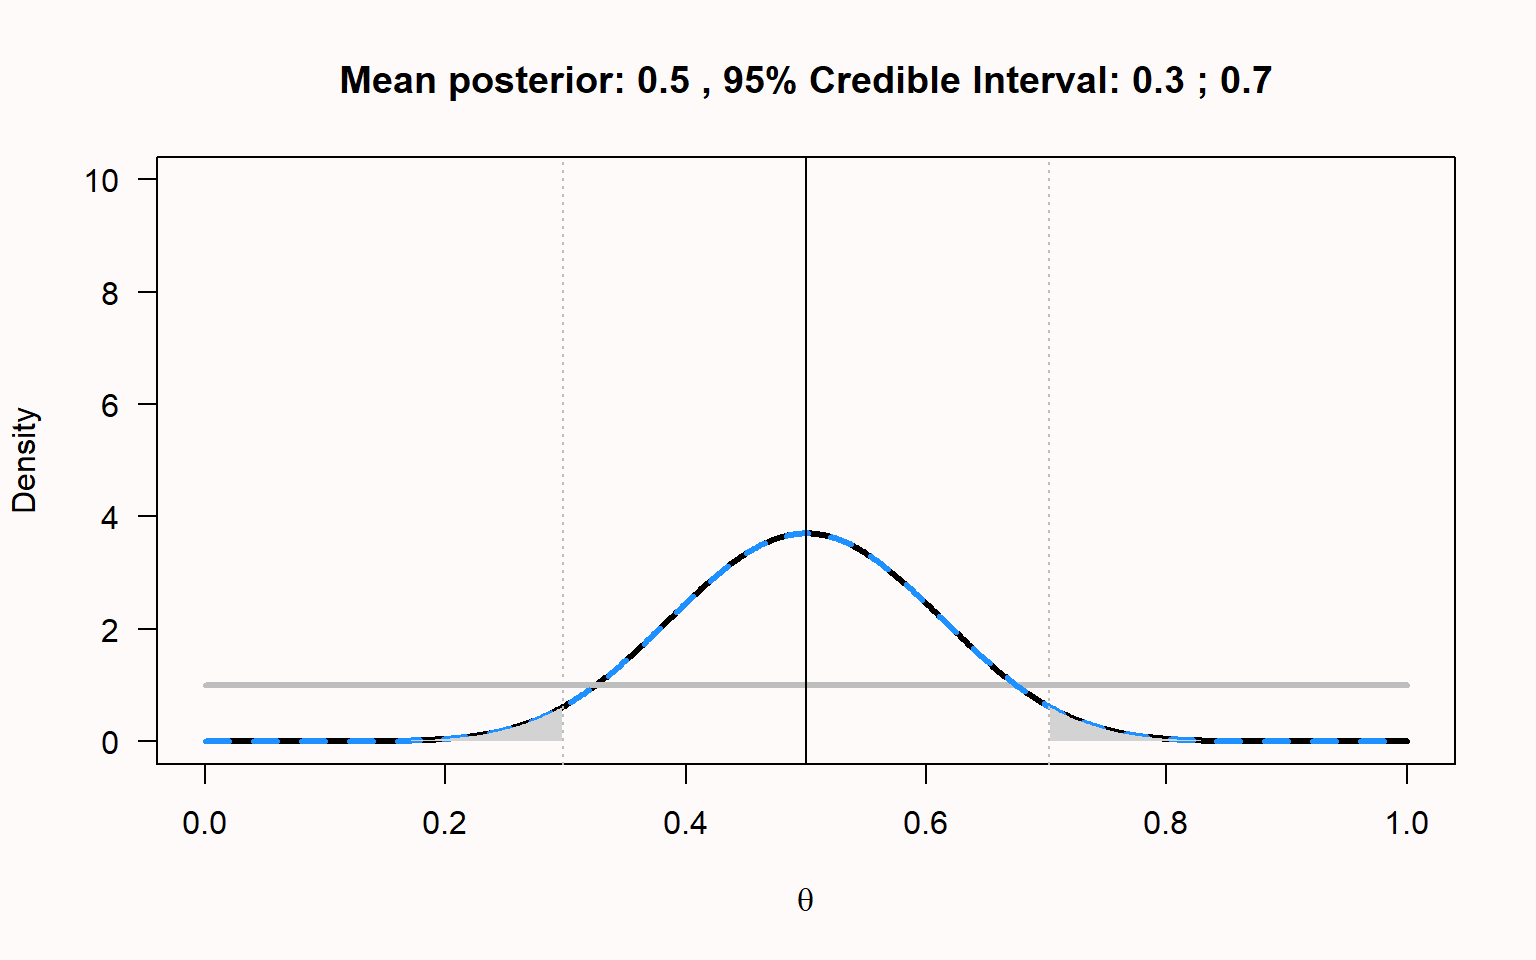
\includegraphics[width=1\linewidth]{04-bayes_files/figure-latex/bayes8-1} 

}

\caption{Plot for the mean of the posterior when 10 out of 20 heads are observed given a uniform prior.}\label{fig:bayes8}
\end{figure}

We can also use the `binom' package to calculate the posterior mean, credible interval, and \textbf{highest density interval (HDI)}. The highest density interval is an alternative to the credible interval that works better when the posterior beta distribution is skewed (and is identical when the posterior distribution is symmetrical. We won't go into the calculations of the HDI here.

\begin{Shaded}
\begin{Highlighting}[]
\FunctionTok{library}\NormalTok{(binom)}

\NormalTok{n }\OtherTok{\textless{}{-}} \DecValTok{20} \CommentTok{\# set total trials}
\NormalTok{x }\OtherTok{\textless{}{-}} \DecValTok{10} \CommentTok{\# set successes}
\NormalTok{aprior }\OtherTok{\textless{}{-}} \DecValTok{1} \CommentTok{\# Set the alpha for the Beta distribution for the prior}
\NormalTok{bprior }\OtherTok{\textless{}{-}} \DecValTok{1} \CommentTok{\# Set the beta for the Beta distribution for the prior}

\FunctionTok{binom.bayes}\NormalTok{(x, n, }\AttributeTok{type =} \StringTok{"central"}\NormalTok{, }\AttributeTok{prior.shape1 =}\NormalTok{ aprior, }\AttributeTok{prior.shape2 =}\NormalTok{ bprior)}
\end{Highlighting}
\end{Shaded}

\begin{verbatim}
##   method  x  n shape1 shape2 mean     lower     upper  sig
## 1  bayes 10 20     11     11  0.5 0.2978068 0.7021932 0.05
\end{verbatim}

\begin{Shaded}
\begin{Highlighting}[]
\FunctionTok{binom.bayes}\NormalTok{(x, n, }\AttributeTok{type =} \StringTok{"highest"}\NormalTok{, }\AttributeTok{prior.shape1 =}\NormalTok{ aprior, }\AttributeTok{prior.shape2 =}\NormalTok{ bprior)}
\end{Highlighting}
\end{Shaded}

\begin{verbatim}
##   method  x  n shape1 shape2 mean     lower     upper  sig
## 1  bayes 10 20     11     11  0.5 0.2978068 0.7021932 0.05
\end{verbatim}

The posterior mean is identical to the Frequentist mean, but this is only the case when the mean of the prior equals the mean of the likelihood \citep{albers_credible_2018}. This chapter shows the essence of Bayesian inference, where we decide upon a prior distribution, collect data and calculate a marginal likelihood, and use these to calculate a posterior distribution. From this posterior distribution, we can estimate the mean and the 95\% credible interval. For any specific hypothesis, we can calculate the relative evidence for a posterior model, compared to a prior model, through the Bayes Factor. There are many different flavors of Bayesian statistics, and the disagreements between Bayesians about what the best approach to statistical inferences is, is at least as great as the disagreements between frequentists and Bayesians, and many Bayesians dislike Bayes factors \citep{mcelreath_statistical_2016}. For example, some Bayesians dislike subjective priors as used in \textbf{subjective Bayesian analysis}, and instead prefer what is known as \textbf{objective Bayesian analysis} \citep{berger_interplay_2004}. In your research, you will most likely need other calculations than the binomial example we have used here, and a lot of Bayesian tests are now available in the free open source software package \href{https://jasp-stats.org/}{JASP}. The math and the priors become more complex, but the basic idea remains the same. You can use Bayesian statistics to quantify relative evidence, which can inform you how much we should believe, or update our beliefs, in theories.

\hypertarget{test-yourself-3}{%
\section{Test Yourself}\label{test-yourself-3}}

\textbf{Q1}: The true believer had a prior of Beta(1,0.5). After observing 10 heads out of 20 coin flips, what is the posterior distribution, given that α* = α + x and β* = β + n -- x?

\begin{enumerate}
\def\labelenumi{\Alph{enumi})}
\tightlist
\item
  Beta(10, 10)
\item
  Beta(11, 10.5)
\item
  Beta(10, 20)
\item
  Beta(11, 20.5)
\end{enumerate}

\textbf{Q2}: The strong skeptic had a prior of Beta(100,100). After observing 50 heads out of 100 coin flips, what is the posterior distribution, given that α* = α + x and β* = β + n -- x?

\begin{enumerate}
\def\labelenumi{\Alph{enumi})}
\tightlist
\item
  Beta(50, 50)
\item
  Beta(51, 51)
\item
  Beta(150, 150)
\item
  Beta(151, 151)
\end{enumerate}

Copy the R script below into R. This script requires 5 input parameters (identical to the Bayes Factor calculator website used above). These are the hypothesis you want to examine (e.g., when evaluating whether a coin is fair, \emph{p} = 0.5), the total number of trials (e.g., 20 flips), the number of successes (e.g., 10 heads), and the \(\alpha\) and \(\beta\) values for the Beta distribution for the prior (e.g., \(\alpha\) = 1 and \(\beta\) = 1 for a uniform prior). Run the script. It will calculate the Bayes Factor, and plot the prior (grey), likelihood (dashed blue) and posterior (black).

\begin{Shaded}
\begin{Highlighting}[]
\NormalTok{H0 }\OtherTok{\textless{}{-}} \FloatTok{0.5} \CommentTok{\# Set the point null hypothesis you want to calculate the Bayes Factor for}
\NormalTok{n }\OtherTok{\textless{}{-}} \DecValTok{20} \CommentTok{\# set total trials}
\NormalTok{x }\OtherTok{\textless{}{-}} \DecValTok{10} \CommentTok{\# set successes}
\NormalTok{aprior }\OtherTok{\textless{}{-}} \DecValTok{1} \CommentTok{\# Set the alpha for the Beta distribution for the prior}
\NormalTok{bprior }\OtherTok{\textless{}{-}} \DecValTok{1} \CommentTok{\# Set the beta for the Beta distribution for the prior}

\NormalTok{alikelihood }\OtherTok{\textless{}{-}}\NormalTok{ x }\SpecialCharTok{+} \DecValTok{1} \CommentTok{\# Calculate the alpha for the Beta distribution for the likelihood}
\NormalTok{blikelihood }\OtherTok{\textless{}{-}}\NormalTok{ n }\SpecialCharTok{{-}}\NormalTok{ x }\SpecialCharTok{+} \DecValTok{1} \CommentTok{\# Calculate the beta for the Beta distribution for the likelihood}
\NormalTok{aposterior }\OtherTok{\textless{}{-}}\NormalTok{ aprior }\SpecialCharTok{+}\NormalTok{ alikelihood }\SpecialCharTok{{-}} \DecValTok{1} \CommentTok{\# Calculate the alpha for the Beta distribution for the posterior}
\NormalTok{bposterior }\OtherTok{\textless{}{-}}\NormalTok{ bprior }\SpecialCharTok{+}\NormalTok{ blikelihood }\SpecialCharTok{{-}} \DecValTok{1} \CommentTok{\# Calculate the beta for the Beta distribution for the posterior}

\NormalTok{theta }\OtherTok{\textless{}{-}} \FunctionTok{seq}\NormalTok{(}\DecValTok{0}\NormalTok{, }\DecValTok{1}\NormalTok{, }\FloatTok{0.001}\NormalTok{) }\CommentTok{\#create probability range p from 0 to 1}
\NormalTok{prior }\OtherTok{\textless{}{-}} \FunctionTok{dbeta}\NormalTok{(theta, aprior, bprior)}
\NormalTok{likelihood }\OtherTok{\textless{}{-}} \FunctionTok{dbeta}\NormalTok{(theta, alikelihood, blikelihood)}
\NormalTok{posterior }\OtherTok{\textless{}{-}} \FunctionTok{dbeta}\NormalTok{(theta, aposterior, bposterior)}

\CommentTok{\# Create plot}
\FunctionTok{plot}\NormalTok{(theta, posterior, }\AttributeTok{ylim =} \FunctionTok{c}\NormalTok{(}\DecValTok{0}\NormalTok{, }\DecValTok{15}\NormalTok{), }\AttributeTok{type =} \StringTok{"l"}\NormalTok{, }\AttributeTok{lwd =} \DecValTok{3}\NormalTok{, }\AttributeTok{xlab =} \StringTok{"p"}\NormalTok{, }\AttributeTok{ylab =} \StringTok{"Density"}\NormalTok{, }\AttributeTok{las =} \DecValTok{1}\NormalTok{)}
\FunctionTok{lines}\NormalTok{(theta, prior, }\AttributeTok{col =} \StringTok{"grey"}\NormalTok{, }\AttributeTok{lwd =} \DecValTok{3}\NormalTok{)}
\FunctionTok{lines}\NormalTok{(theta, likelihood, }\AttributeTok{lty =} \DecValTok{2}\NormalTok{, }\AttributeTok{lwd =} \DecValTok{3}\NormalTok{, }\AttributeTok{col =} \StringTok{"dodgerblue"}\NormalTok{)}
\NormalTok{BF10 }\OtherTok{\textless{}{-}} \FunctionTok{dbeta}\NormalTok{(H0, aposterior, bposterior) }\SpecialCharTok{/} \FunctionTok{dbeta}\NormalTok{(H0, aprior, bprior)}
\FunctionTok{points}\NormalTok{(H0, }\FunctionTok{dbeta}\NormalTok{(H0, aposterior, bposterior), }\AttributeTok{pch =} \DecValTok{19}\NormalTok{)}
\FunctionTok{points}\NormalTok{(H0, }\FunctionTok{dbeta}\NormalTok{(H0, aprior, bprior), }\AttributeTok{pch =} \DecValTok{19}\NormalTok{, }\AttributeTok{col =} \StringTok{"grey"}\NormalTok{)}
\FunctionTok{segments}\NormalTok{(H0, }\FunctionTok{dbeta}\NormalTok{(H0, aposterior, bposterior), H0, }\FunctionTok{dbeta}\NormalTok{(H0, aprior, bprior), }\AttributeTok{lty =} \DecValTok{2}\NormalTok{)}
\FunctionTok{title}\NormalTok{(}\FunctionTok{paste}\NormalTok{(}\StringTok{"Bayes Factor:"}\NormalTok{, }\FunctionTok{round}\NormalTok{(BF10, }\AttributeTok{digits =} \DecValTok{2}\NormalTok{)))}
\end{Highlighting}
\end{Shaded}

\begin{center}\includegraphics[width=1\linewidth]{04-bayes_files/figure-latex/unnamed-chunk-3-1} \end{center}

We see that for the newborn, \emph{p} = 0.5 has become more probable, but so has \emph{p} = 0.4.

\textbf{Q3}: Change the hypothesis in the first line from 0.5 to 0.675, and run the script. If you were testing the idea that this coin returns 67.5\% heads, which statement is true?

\begin{enumerate}
\def\labelenumi{\Alph{enumi})}
\tightlist
\item
  Your belief in this hypothesis, given the data, would have decreased.
\item
  Your belief in this hypothesis, given the data, would have stayed the same.
\item
  Your belief in this hypothesis, given the data, would have increased.
\end{enumerate}

\textbf{Q4}: Change the hypothesis in the first line back to 0.5. Let's look at the increase in the belief of the hypothesis \emph{p} = 0.5 for the strong skeptic after 10 heads out of 20 coin flips. Change the \(\alpha\) for the prior in line 4 to 100 and the \(\beta\) for the prior in line 5 to 100. Run the script. Compare the Figure from R to the increase in belief for the newborn (in the plot on the previous page). Which statement is true?

\begin{enumerate}
\def\labelenumi{\Alph{enumi})}
\tightlist
\item
  The belief in the hypothesis that \emph{p} = 0.5, given the data, has \textbf{increased} for the strong skeptic, but \textbf{not} as much as it has for the newborn.
\item
  The belief in the hypothesis that \emph{p} = 0.5, given the data, has \textbf{increased} for the strong skeptic, \textbf{exactly as much} as it has for the newborn.
\item
  The belief in the hypothesis that \emph{p} = 0.5, given the data, has \textbf{increased} for the strong skeptic, and \textbf{much more} than it has for the newborn.
\item
  The belief in the hypothesis that \emph{p} = 0.5, given the data, has \textbf{decreased} for the strong skeptic.
\end{enumerate}

Copy the R script below and run it. The script will plot the mean for the posterior when 10 heads out of 20 coin flips are observed, given a uniform prior (as in \ref{fig:bayes8}) . The script will also use the `binom' package to calculate the posterior mean, credible interval, and \textbf{highest density interval (HDI)}. The highest density interval is an alternative to the credible interval that works better when the posterior beta distribution is skewed (and is identical when the posterior distribution is symmetrical. We won't go into the calculations of the HDI here.

\begin{Shaded}
\begin{Highlighting}[]
\NormalTok{n }\OtherTok{\textless{}{-}} \DecValTok{20} \CommentTok{\# set total trials}
\NormalTok{x }\OtherTok{\textless{}{-}} \DecValTok{10} \CommentTok{\# set successes}
\NormalTok{aprior }\OtherTok{\textless{}{-}} \DecValTok{1} \CommentTok{\# Set the alpha for the Beta distribution for the prior}
\NormalTok{bprior }\OtherTok{\textless{}{-}} \DecValTok{1} \CommentTok{\# Set the beta for the Beta distribution for the prior}

\NormalTok{ymax }\OtherTok{\textless{}{-}} \DecValTok{10} \CommentTok{\# set max y{-}axis}

\NormalTok{alikelihood }\OtherTok{\textless{}{-}}\NormalTok{ x }\SpecialCharTok{+} \DecValTok{1} \CommentTok{\# Calculate the alpha for the Beta distribution for the likelihood}
\NormalTok{blikelihood }\OtherTok{\textless{}{-}}\NormalTok{ n }\SpecialCharTok{{-}}\NormalTok{ x }\SpecialCharTok{+} \DecValTok{1} \CommentTok{\# Calculate the beta for the Beta distribution for the likelihood}
\NormalTok{aposterior }\OtherTok{\textless{}{-}}\NormalTok{ aprior }\SpecialCharTok{+}\NormalTok{ alikelihood }\SpecialCharTok{{-}} \DecValTok{1} \CommentTok{\# Calculate the alpha for the Beta distribution for the posterior}
\NormalTok{bposterior }\OtherTok{\textless{}{-}}\NormalTok{ bprior }\SpecialCharTok{+}\NormalTok{ blikelihood }\SpecialCharTok{{-}} \DecValTok{1} \CommentTok{\# Calculate the beta for the Beta distribution for the posterior}

\NormalTok{theta }\OtherTok{\textless{}{-}} \FunctionTok{seq}\NormalTok{(}\DecValTok{0}\NormalTok{, }\DecValTok{1}\NormalTok{, }\FloatTok{0.001}\NormalTok{) }\CommentTok{\# create probability range p from 0 to 1}
\NormalTok{prior }\OtherTok{\textless{}{-}} \FunctionTok{dbeta}\NormalTok{(theta, aprior, bprior) }\CommentTok{\# deterine prior distribution}
\NormalTok{likelihood }\OtherTok{\textless{}{-}} \FunctionTok{dbeta}\NormalTok{(theta, alikelihood, blikelihood) }\CommentTok{\# determine likelihood distribution}
\NormalTok{posterior }\OtherTok{\textless{}{-}} \FunctionTok{dbeta}\NormalTok{(theta, aposterior, bposterior) }\CommentTok{\# determine posterior distribution}
\FunctionTok{plot}\NormalTok{(theta, posterior, }\AttributeTok{ylim =} \FunctionTok{c}\NormalTok{(}\DecValTok{0}\NormalTok{, ymax), }\AttributeTok{type =} \StringTok{"l"}\NormalTok{, }\AttributeTok{lwd =} \DecValTok{3}\NormalTok{, }\AttributeTok{xlab =} \FunctionTok{bquote}\NormalTok{(theta), }\AttributeTok{ylab =} \StringTok{"Density"}\NormalTok{, }\AttributeTok{las =} \DecValTok{1}\NormalTok{) }\CommentTok{\# draw posterior distribution}
\FunctionTok{lines}\NormalTok{(theta, prior, }\AttributeTok{col =} \StringTok{"grey"}\NormalTok{, }\AttributeTok{lwd =} \DecValTok{3}\NormalTok{) }\CommentTok{\# draw prior distribution}
\FunctionTok{lines}\NormalTok{(theta, likelihood, }\AttributeTok{lty =} \DecValTok{2}\NormalTok{, }\AttributeTok{lwd =} \DecValTok{3}\NormalTok{, }\AttributeTok{col =} \StringTok{"dodgerblue"}\NormalTok{) }\CommentTok{\# draw likelihood distribution}
\NormalTok{LL }\OtherTok{\textless{}{-}} \FunctionTok{qbeta}\NormalTok{(.}\DecValTok{025}\NormalTok{, aposterior, bposterior) }\CommentTok{\# calculate lower limit credible interval}
\NormalTok{UL }\OtherTok{\textless{}{-}} \FunctionTok{qbeta}\NormalTok{(.}\DecValTok{975}\NormalTok{, aposterior, bposterior) }\CommentTok{\# calculate upper limit credible interval}
\FunctionTok{abline}\NormalTok{(}\AttributeTok{v =}\NormalTok{ aposterior }\SpecialCharTok{/}\NormalTok{ (aposterior }\SpecialCharTok{+}\NormalTok{ bposterior)) }\CommentTok{\# draw line mean}
\FunctionTok{abline}\NormalTok{(}\AttributeTok{v =}\NormalTok{ LL, }\AttributeTok{col =} \StringTok{"grey"}\NormalTok{, }\AttributeTok{lty =} \DecValTok{3}\NormalTok{) }\CommentTok{\# draw line lower limit}
\FunctionTok{abline}\NormalTok{(}\AttributeTok{v =}\NormalTok{ UL, }\AttributeTok{col =} \StringTok{"grey"}\NormalTok{, }\AttributeTok{lty =} \DecValTok{3}\NormalTok{) }\CommentTok{\# draw line upper limit}
\FunctionTok{polygon}\NormalTok{(}\FunctionTok{c}\NormalTok{(theta[theta }\SpecialCharTok{\textless{}}\NormalTok{ LL], }\FunctionTok{rev}\NormalTok{(theta[theta }\SpecialCharTok{\textless{}}\NormalTok{ LL])), }\FunctionTok{c}\NormalTok{(posterior[theta }\SpecialCharTok{\textless{}}\NormalTok{ LL], }\FunctionTok{rep}\NormalTok{(}\DecValTok{0}\NormalTok{, }\FunctionTok{sum}\NormalTok{(theta }\SpecialCharTok{\textless{}}\NormalTok{ LL))), }\AttributeTok{col =} \StringTok{"lightgrey"}\NormalTok{, }\AttributeTok{border =} \ConstantTok{NA}\NormalTok{)}
\FunctionTok{polygon}\NormalTok{(}\FunctionTok{c}\NormalTok{(theta[theta }\SpecialCharTok{\textgreater{}}\NormalTok{ UL], }\FunctionTok{rev}\NormalTok{(theta[theta }\SpecialCharTok{\textgreater{}}\NormalTok{ UL])), }\FunctionTok{c}\NormalTok{(posterior[theta }\SpecialCharTok{\textgreater{}}\NormalTok{ UL], }\FunctionTok{rep}\NormalTok{(}\DecValTok{0}\NormalTok{, }\FunctionTok{sum}\NormalTok{(theta }\SpecialCharTok{\textgreater{}}\NormalTok{ UL))), }\AttributeTok{col =} \StringTok{"lightgrey"}\NormalTok{, }\AttributeTok{border =} \ConstantTok{NA}\NormalTok{)}
\FunctionTok{title}\NormalTok{(}\FunctionTok{paste}\NormalTok{(}\StringTok{"Mean posterior:"}\NormalTok{, }\FunctionTok{round}\NormalTok{((aposterior }\SpecialCharTok{/}\NormalTok{ (aposterior }\SpecialCharTok{+}\NormalTok{ bposterior)), }\AttributeTok{digits =} \DecValTok{5}\NormalTok{), }\StringTok{", 95\% Credible Interval:"}\NormalTok{, }\FunctionTok{round}\NormalTok{(LL, }\AttributeTok{digits =} \DecValTok{2}\NormalTok{), }\StringTok{";"}\NormalTok{, }\FunctionTok{round}\NormalTok{(UL, }\AttributeTok{digits =} \DecValTok{2}\NormalTok{)))}
\end{Highlighting}
\end{Shaded}

\begin{center}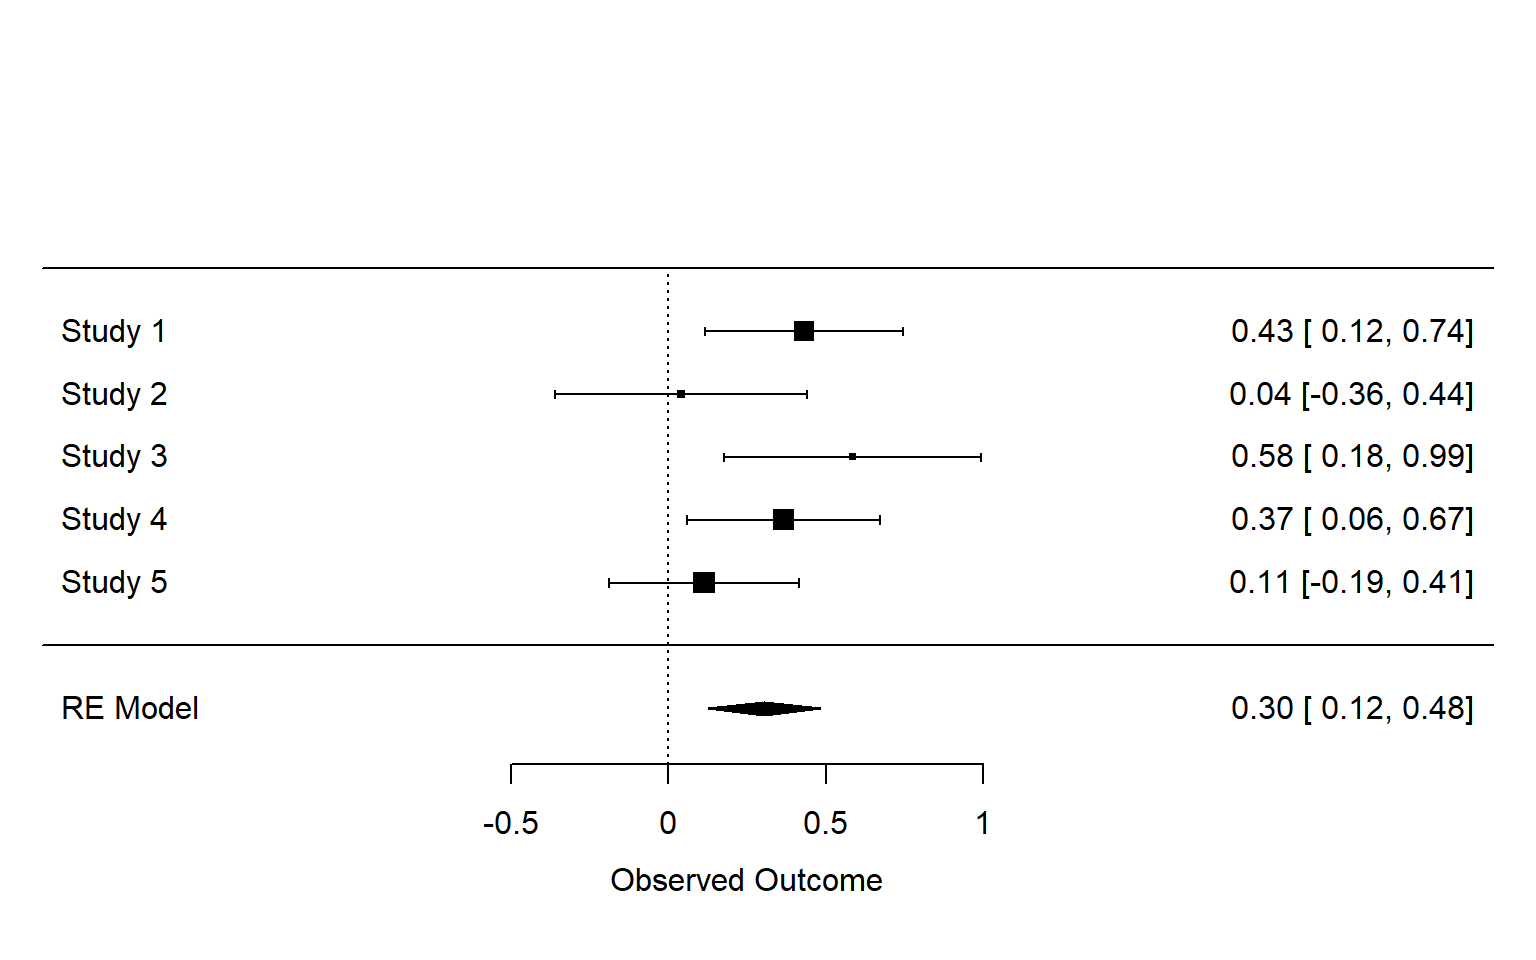
\includegraphics[width=1\linewidth]{04-bayes_files/figure-latex/unnamed-chunk-4-1} \end{center}

\begin{Shaded}
\begin{Highlighting}[]
\ControlFlowTok{if}\NormalTok{ (}\SpecialCharTok{!}\FunctionTok{require}\NormalTok{(binom)) \{}
  \FunctionTok{install.packages}\NormalTok{(}\StringTok{"binom"}\NormalTok{)}
\NormalTok{\}}
\FunctionTok{library}\NormalTok{(binom)}
\FunctionTok{binom.bayes}\NormalTok{(x, n, }\AttributeTok{type =} \StringTok{"central"}\NormalTok{, }\AttributeTok{prior.shape1 =}\NormalTok{ aprior, }\AttributeTok{prior.shape2 =}\NormalTok{ bprior)}
\end{Highlighting}
\end{Shaded}

\begin{verbatim}
##   method  x  n shape1 shape2 mean     lower     upper  sig
## 1  bayes 10 20     11     11  0.5 0.2978068 0.7021932 0.05
\end{verbatim}

\begin{Shaded}
\begin{Highlighting}[]
\FunctionTok{binom.bayes}\NormalTok{(x, n, }\AttributeTok{type =} \StringTok{"highest"}\NormalTok{, }\AttributeTok{prior.shape1 =}\NormalTok{ aprior, }\AttributeTok{prior.shape2 =}\NormalTok{ bprior)}
\end{Highlighting}
\end{Shaded}

\begin{verbatim}
##   method  x  n shape1 shape2 mean     lower     upper  sig
## 1  bayes 10 20     11     11  0.5 0.2978068 0.7021932 0.05
\end{verbatim}

The posterior mean is identical to the Frequentist mean, but this is only the case when the mean of the prior equals the mean of the likelihood.

\textbf{Q5}: Assume the outcome of 20 coin flips had been 18 heads. Change x to 18 in line 2 and run the script. Remember that the mean of the prior Beta(1,1) distribution is α/(α+β), or 1/(1+1) = 0.5. The Frequentist mean is simply x/n, or 18/20=0.9. Which statement is true?

\begin{enumerate}
\def\labelenumi{\Alph{enumi})}
\tightlist
\item
  The frequentist mean is \textbf{higher} than the mean of the posterior, because the mean of the posterior is \textbf{closer} to the mean of the prior distribution.
\item
  The frequentist mean is \textbf{lower} than the mean of the posterior, because the mean of the posterior is \textbf{closer} to the mean of the prior distribution.
\item
  The frequentist mean is \textbf{higher} than the mean of the posterior, because the mean of the posterior is \textbf{further from} to the mean of the prior distribution.
\item
  The frequentist mean is \textbf{lower} than the mean of the posterior, because the mean of the posterior is \textbf{further from} to the mean of the prior distribution.
\end{enumerate}

\textbf{Q6}: What is, today, your best estimate of the probability that the sun rises every day? Assume you were born with an uniform Beta(1,1) prior. The sun can either rise, or it does not. Assume you have seen the sun every day since you were born, which means there has been a continuous string of successes for every day you have been alive. It is ok to estimate the days you have been alive by just multiplying your age by 365 days. What is your best estimate of the probability that the sun will rise?

\textbf{Q7}: What would have been the best estimate from a Frequentist perspective?

\textbf{Q8}: What do you think the goal of science is? Rozeboom \citeyearpar{rozeboom_fallacy_1960} has criticized Neyman-Pearson hypothesis testing by stating:

\begin{quote}
But the primary aim of a scientific experiment is not to precipitate decisions, but to make an appropriate adjustment in the degree to which one accepts, or believes, the hypothesis or hypotheses being tested''.
\end{quote}

Frick \citeyearpar{frick_appropriate_1996} has argued against Rozeboom, by stating:

\begin{quote}
Rozeboom (1960) suggested that scientists should not be making decisions about claims, they should be calculating and updating the probability of these claims. However, this does not seem practical. If there were only a handful of potential claims in any given area of psychology, it would be feasible to assign them probabilities, to be constantly updating the probabilities, and to expect experimenters to keep track of these ever-changing probabilities. In fact, just the number of claims in psychology is overwhelming. It would probably be impossible for human beings to keep track of the probability for each claim, especially if these probabilities were constantly changing. In any case, scientists do not assign probabilities to claims. Instead, scientists act like the goal of science is to collect a corpus of claims that are considered to be established (Giere, 1972).
\end{quote}

When it comes to philosophy of science, there are no right or wrong answers. Reflect in 250 words on your thoughts about the two goals of science outlines by Rozeboom and Frick, and how these relate to your philosophy of science.

\hypertarget{questions}{%
\chapter{Asking Statistical Questions}\label{questions}}

At the core of the design of a new study is the evaluation of its \textbf{information quality}: the potential of a particular dataset for achieving a given analysis goal by employing data analysis methods and considering a given utility
\citep{kenett_information_2016}. The goal of data collection is to gain information through \textbf{empirical research} where observations are collected and analyzed, often through statistical models. Three approaches to statistical modelling can be distinguished \citet{shmueli_explain_2010}: Description, explanation, and prediction, which are discussed below. The utility often depends on which effects are deemed interesting. A thorough evaluation of the informatin quality of a study therefore depends on clearly specifying the goal of data collection, the statistical modelling approach that is chosen, and the usefulness of the data to draw conclusions about effects of interest with the chosen analysis method. A study with low information quality might not be worth performing, as the data that will be collected has low potential to achieve the analysis goal.

\hypertarget{description}{%
\section{Description}\label{description}}

Description aims to answer questions about features of the empirical manifestation of some phenomenon. Description can involve unique events (e.g., case studies of single patients), classes of events (e.g., patients with a certain disease). Examples of features of interest are duration (how long), quantity (how many), location (where), etc.

An example of a descriptive question is research by \href{https://en.wikipedia.org/wiki/Kinsey_Reports}{Kinsey}, who studied the sexual behavior and experiences of Americans in a time that very little scientific research was available on this topic. He used interviews that provided the statistical basis to draw conclusions about sexuality in the United States, which, at the time, challenged conventional beliefs about sexuality.

Descriptive research questions are answered through \textbf{estimation statistics}. The informational value of an estimation study is determined by the amount of observations (the more observations, the higher the \textbf{precision} of the estimates) and the sampling plan (the more representative the sample, the lower the \textbf{sample selection bias}, which increases the ability to generalize from the sample to the population), and the reliability of the measure.

Descriptive research questions are sometimes seen as less exciting than explanation or prediction questions \citep{gerring_mere_2012}, but they are essential building block of theory formation \citep{scheel_why_2021}. Although estimation question often focus on the mean score of a measure, accurate estimates of the variance of a measure are extremely valuable as well. The variance of a measure is essential information in a well-informed sample size justification, both when planning for accuracy, as when performing an a-priori power analysis.

\hypertarget{prediction}{%
\section{Prediction}\label{prediction}}

The goal in predictive modeling is to apply an algorithm or a statistical model to predict future observations \citep{shmueli_explain_2010}. For example, during the COVID-9 pandemic a large number of models were created that combined variables to estimate the risk that people would be infected with COVID, or that people who were infected would experience negative effects on their health \citep{wynants_prediction_2020}. Ideally, the goal is to develop a prediction model that accurately captures the regularities in its training data, and that generalizes well to unseen data. There is a \textbf{bias-variance tradeoff} between these two goals, and researchers need to decide how much bias should be reduced which increases the variance, or vice-versa \citep{yarkoni_choosing_2017}. The goal in prediction is to minimize prediction error. Common methods to evaluate prediction errors is \textbf{cross-validation}, where for example it is examined whether a model developed on a training dataset generalizes to a holdout dataset. The development of prediction models is becoming increasingly popular with the rise of machine learning approaches.

\hypertarget{explanation}{%
\section{Explanation}\label{explanation}}

The use of statistical models concerns tests of explanatory theories. In this case, statistical models are used to test causal assumptions, or explanations that we derive from theories.
Meehl \citeyearpar{meehl_appraising_1990} reminds us of the important distinction between a substantive theory, a statistical hypothesis, and observations. Statistical inference is only involved in drawing conclusions about the statistical hypothesis. Observations can lead to the conclusion that the statistical hypothesis is is confirmed (or not), but this conclusion does not directly translate into corroboration for the theory.

We never test a theory in isolation, but always include auxiliary hypotheses about the measures and instruments that are used in a study, conditions realized in the experiment, to the \textbf{ceteris paribus} clause that assumes all other things are equal. Therefore, it is never clear if a failure to corroborate a theoretical prediction should be blamed on the theory or the auxiliary hypotheses. To generate reliable explanatory theories, researchers therefore have to perform lines of research in which auxiliary hypotheses are systematically tested \citep{tunc_falsificationist_2020}.

\begin{figure}

{\centering 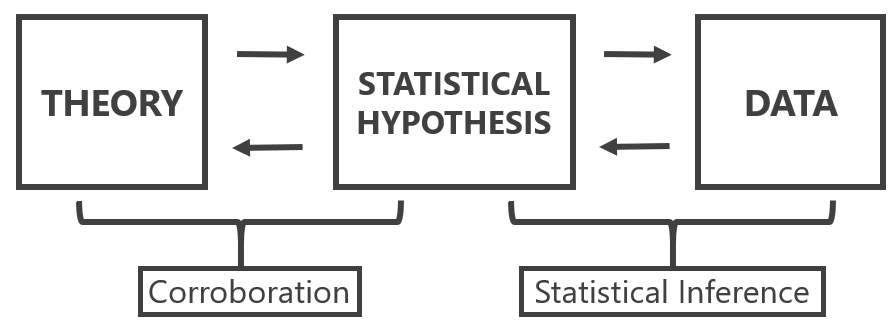
\includegraphics[width=1\linewidth]{images/meehl1990} 

}

\caption{Distinction between a theoretical hypothesis, a statistical hypothesis, and observations. Figure based on Meehl, 1990.}\label{fig:meehl1990}
\end{figure}

\hypertarget{loosening-and-tightening}{%
\section{Loosening and Tightening}\label{loosening-and-tightening}}

For each of the three questions above, we can ask questions about description, prediction, and explanation during a \textbf{loosening} phase when doing research, or during a \textbf{tightening} phase \citep{fiedler_tools_2004}. The distinction is relative. During the loosening stage, the focus is on creating variation that provides the source for new ideas. During the tightening stage, selection takes place with the goal to distinguish useful variants from less useful variants. In descriptive research, an unstructured interview is more aligned with the loosening phase, while a structured interview is more aligned with the tightening phase. In prediction, building a prediction model based on the training set is the loosening phase, while evaluation the prediction error in the holdout dataset is the tightening phase. In explanation, exploratory experimentation functions to generate hypotheses, while hypothesis tests function to distinguish theories that make predictions that are corroborated from those theories which predictions are not corroborated.

It is important to realize whether your goal is to generate new ideas, or to test new ideas. Researchers are often not explicit about the stage their research is in, which runs the risk of trying to test hypotheses prematurely \citep{scheel_why_2021}. Clinical trials research is more explicit about the different phases of research, and distinguishes Phase 1, Phase 2, Phase 3, and Phase 4 trials. In a Phase 1 trial researchers evaluate the safety of a new drug or intervention in a small group of non-randomized (often healthy) volunteers, by examining how much of a drug is safe to give, while monitoring a range of possible side effects. A phase 2 trial are often performed with patients as participants, and can focus in more detail on finding the definite dose. The goal is to systematically explore a range of parameters (e.g., the intensity of a stimulus) to identify boundary conditions \citep{dubin_theory_1969}. A phase 3 trial is a large randomized controlled trial with the goal to test the effectiveness of the new intervention in practice. Phase 3 trials require a prespecified statistical analyses plan that strictly controls error rates. Finally, a Phase 4 trial examines long term safety and generalizability. Compared to a Phase 3 trial, there is more loosening, as researchers explore the possibility of interactions with other drugs, or moderating effects in certain subgroups of the population. In clinical trials, a Phase 3 trial requires a huge amount of preparation, and is not undertaken lightly.

\begin{figure}

{\centering 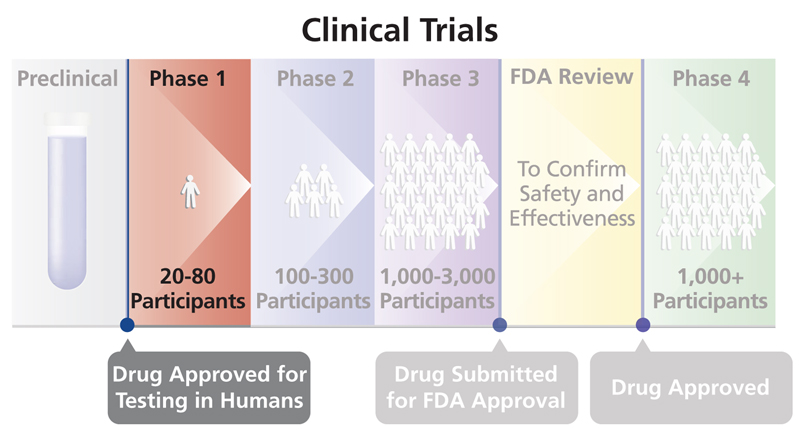
\includegraphics[width=1\linewidth]{images/trialphase} 

}

\caption{Four phases of clinical research. <a href="https://clinicalinfo.hiv.gov/en/glossary/phase-1-trial">Source</a>.}\label{fig:trialphase}
\end{figure}

\hypertarget{three-statistical-philosophies}{%
\section{Three statistical philosophies}\label{three-statistical-philosophies}}

Royall \citeyearpar{royall_statistical_1997} distinguishes three questions one can ask:

\begin{enumerate}
\def\labelenumi{\arabic{enumi}.}
\tightlist
\item
  What do I believe, now that I have this observation?
\item
  What should I do, now that I have this observation?
\item
  What does this observation tell me about A versus B? (How should I interpret this observation as evidence regarding A versus B?)
\end{enumerate}

One useful metaphor that think about these differences is if we look at Hinduism, where there are three ways to reach enlightenment: The Bhakti yoga, or the Path of Devotion, the Karma yoga, or the Path of Action, the Jnana yoga, or the Path of Knowledge. The three corresponding statistical paths are Bayesian statistics, which focuses on updating beliefs, Neyman-Pearson statistics, which focuses on making decisions about how to act, and likelihood approaches, which focus on quantifying the evidence or knowledge gained from the data. Just like in Hinduism the different paths are not mutually exclusive, and the emphasis on these three yoga's differs between individuals, so will scientists differ in their emphasis of their preferred approach to statistics.

The three approaches to statistical modelling (description, prediction, and explanation) can be examined from each the three statistical philosophies (e.g., frequentist estimation, maximum likelihood estimation, and Bayesian estimation, or Neyman-Pearson hypothesis tests, likelihood ratio tests, and Bayes factors). Bayesian approaches start from a specified prior belief, and use the data to update their belief. Frequentist procedures focus on methodological procedures that allow researchers to make inferences that control the probability of error in the long run. Likelihood approaches focus on quantifying the evidential value in the observed data. When used knowledgeably, these approaches often yield very similar inferences \citep{dongen_multiple_2019, lakens_improving_2020, tendeiro_review_2019}. Jeffreys \citeyearpar{jeffreys_theory_1939}, who developed a Bayesian hypothesis test, noted the following when comparing his Bayesian hypothesis test against frequentist methods proposed by Fisher:

\begin{quote}
I have in fact been struck repeatedly in my own work, after being led on general principles to a solution of a problem, to find that Fisher had already grasped the essentials by some brilliant piece of common sense, and that his results would be either identical with mine or would differ only in cases where we should both be very doubtful. As a matter of fact I have applied my significance tests to numerous applications that have also been worked out by Fisher's, and have not yet found a disagreement in the actual decisions reached.
\end{quote}

At the same time, each approach is based on different principles, and allows for specific inferences. For example, a Neyman-Pearson approach does not quantify evidence, and a Bayesian approach can lead conclusions about the relative support for one over another hypothesis, given specified priors, while ignoring the rate at which such a conclusion would be misleading. Understanding these basic principles is useful, as criticisms on statistical practices (e.g., computing \emph{p}-values) always boil down to a disagreement about the principles that different statistical philosophies are built on. However, when we survey the literature, we rarely see the viewpoint that all approaches to statistical inferences, including p values, provide answers to specific questions a researcher might want to ask. Instead, statisticians often engage in what I call the \textbf{statistician's
fallacy} --- a declaration of what they believe researchers really ``want to know'' without limiting the usefulness of their preferred statistical question to a specific context \citep{lakens_practical_2021}. The most well-known example of the statistician's fallacy is provided by Cohen \citeyearpar{cohen_earth_1994} when discussing null-hypothesis significance testing:

\begin{quote}
What's wrong with NHST? Well, among many other things, it does not tell us what we want to know, and we so much want to know what we want to know that, out of desperation, we nevertheless believe that it does! What we want to know is `Given these data, what is the probability that H0 is true?'
\end{quote}

Different statisticians will argue what you actually ``want to know'' is the posterior probability of a hypothesis, the false-positive risk, the effect size and its confidence interval, the likelihood, the Bayes factor, or the severity with which a hypothesis has been tested. However, it is up to you to choose a statistical strategy that matches the question you want the ask \citep{hand_deconstructing_1994}.

\hypertarget{do-you-really-want-to-test-a-hypothesis}{%
\section{Do You Really Want to Test a Hypothesis?}\label{do-you-really-want-to-test-a-hypothesis}}

A hypothesis test is a very specific answer to a very specific question. We can use a dart game as a metaphor for the question a hypothesis test aims to answer. In essence, both a dart game and a hypothesis test are a methodological procedure to make a directional prediction: Is A better or worse than B?, In a dart game we very often compare two players, and the question is whether we should act as is player A is the best, or player B is the best. In a hypothesis test, we compare two hypotheses, and the question is whether we should act as if the null hypothesis is true, or whether the alternative hypothesis is true.

Historically, researchers have often been interested in testing hypotheses to examine whether predictions that are derived from a scientific theory hold up under scrutiny. Some philosophies of science (but not all) value theories that are able to make predictions. If a darter wants to convince you they are a good player, they can make a prediction (`the next arrow will hit the bulls-eye'), throw a dart, and impress you by hitting the bulls-eye. When a researcher uses a theory to make a prediction, collects data, and observes can claim based on a predefined methodological procedure that the results confirm their prediction, the idea is you are impressed by the \textbf{predictive validity of a theory} \citep{de_groot_methodology_1969}. The test supports the idea that the theory is a useful starting point to generate predictions about reality. Philosophers of science such as Popper call this `verisimilitude'-- the theory is in some way related to the truth, and it has some `truth-likeness'.

In order to be impressed when a prediction is confirmed, the prediction must be able to be wrong. In other words, a theoretical prediction needs to be falsifiable. If our predictions concerned the presence of absence of clearly observable entities (e.g., the existence of a black swan) it is relatively straightforward to divide all possible states of the world into a set that is predicted by our theory (e.g., all swans are white), and a set that is not predicted by our theory (e.g., swans can have other colors than white). However, many scientific questions concern probabilistic events where single observations contain noise due to random variation -- rats have a certain probability to develop a tumor, people have a certain probability to buy a product, or particles have a certain probability to appear after a collision. If we want to forbid certain outcomes of our test when measuring probabilistic events, we can divide the states of the world based on the probability that some result will be observed.

\begin{figure}

{\centering 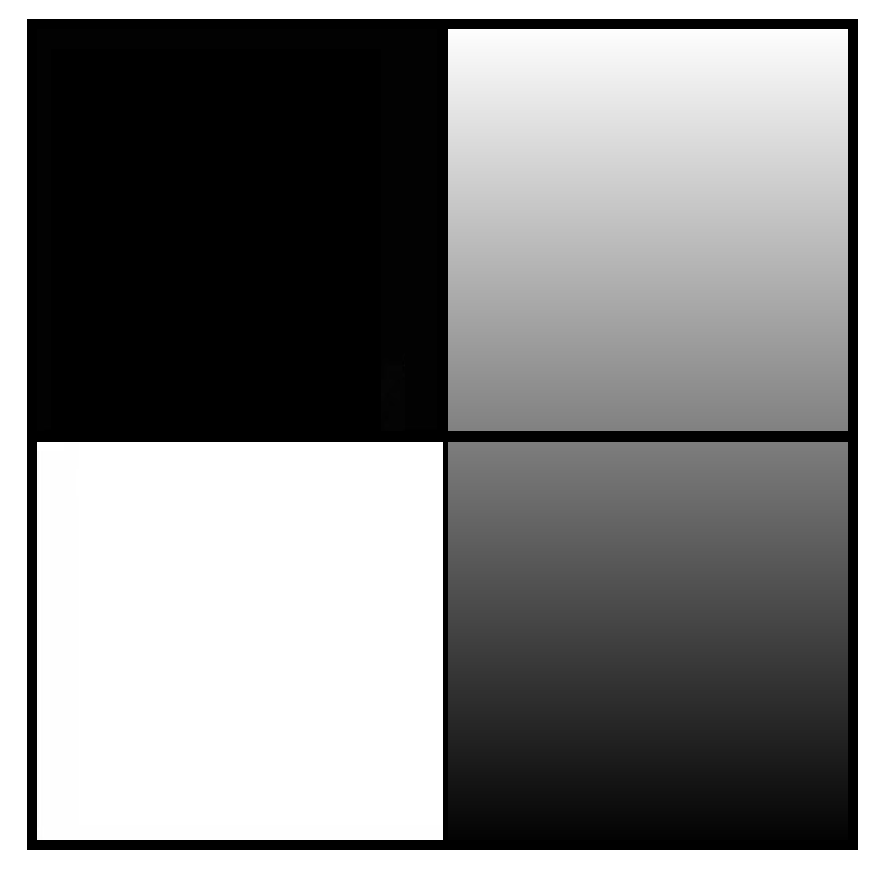
\includegraphics[width=1\linewidth]{images/blackwhite} 

}

\caption{Some fields make black and white predictions about the presence or absence of obervables, but in many sciences, predictions are probabilistic, and shades of grey.}\label{fig:blackwhite}
\end{figure}

Just because a hypothesis test can be performed, does not mean it is interesting. A hypothesis test is most useful when 1) both data generating models that are decided between have some plausibility, and 2) it is possible to apply an informative methodological procedure.

First, the two competing models should both be good players. Just as in a dart game there would be very little interest if I played Michael van Gerwen (the world champion at the time of writing) to decide who the better dart player is. Since I do not play darts very well, a game between the two of us would not be interesting to watch. Similarly, it is sometimes completely uninteresting to compare two data generating models, one representing the state of the world when there is no effect, and another representing the state of the world when there is some effect, because in some cases the absence of an effect is extremely implausible.

Second, for a hypothesis test to be interesting you need to have designed an informative study. When designing a study, you need to be able to make sure that the methodological rule provides a severe test, where you are likely to corroborate a prediction if it is correct, while at the same time fail to corroborate a prediction when it is wrong \citep{mayo_statistical_2018}. If the world champion in darts and I stand 20 inches away from a dart board and can just push the dart in the location where we want it to end up, it is not possible to show my lack of skill. If we are both are blindfolded and throwing the darts from 100 feet, it is not possible for the world champion to display their skill. In a hypothesis test, the statistical severity of a test is determined by the error rates. Therefore, a researcher needs to be able to adequately control error rates to perform a test of a hypothesis with high informational value.

By now it is hopefully clear that a hypothesis tests are a very specific tool, that answer a very specific question: After applying a methodological rule to observed data, which decision should I make if I do not want to make incorrect decisions too often? If you have no desire to use a methodological procedure to decide between competing theories, there is no real reason to report the results of a hypothesis test. Even though it might feel like you should test a hypothesis when doing research, carefully thinking about the statistical question you want to ask might reveal that alternative statistical approaches, such as describing the data you have observed, quantifying your personal beliefs about hypotheses, or reporting the relative likelihood of data under different hypotheses might be the approach that answers the question you really want to know.

\hypertarget{effectsize}{%
\chapter{Effect Sizes}\label{effectsize}}

Effect sizes are an important statistical outcome in most empirical studies. Researchers want to know whether an intervention or experimental manipulation has an effect greater than zero, or (when it is obvious an effect exists) how big the effect is. Researchers are often reminded to report effect sizes, because they are useful for three reasons. First, they allow researchers to present the magnitude of the reported effects, which allow researchers to reflect on the \textbf{practical significance} of the effects they report, in addition to the \emph{statistical} significance. Second, effect sizes allow researchers to draw meta-analytic conclusions by comparing standardized effect sizes across studies. Third, effect sizes from previous studies can be used when planning a new study in an a-priori power analysis.

A measure of effect size is a quantitative description of the strength of a phenomenon. It is expressed as a number on a scale. For \textbf{unstandardized effect sizes}, the effect size is expressed on the scale the measure was collected on. This is useful whenever people are able to intuitively interpret differences on a measurement scale. For example, children grow on average 6 centimeters a year between the age of 2 and puberty. We can interpret 6 centimeters a year as an effect size, and many people in the world have an intuitive understanding of how large 6 cm is. Where a \emph{p}-value is used to make a claim about whether there is an efect, or whether we might just be looking at random variation in the data, an effect size is used to answer the question how large the effect is. This makes an effect size estimate an important complement to \emph{p}-values in most studies. A \emph{p}-value tells use we can claim children grow as they age; effect sizes tell us what size clothes we can expect children to wear when they are a certain age, and how long it will take before their new clothes are too small.

For people in parts of the world that do not use the metric system, if might be difficult to understand what a difference of 6 cm is. To facilitate a comparison of effect sizes across situations where different measurement scales are used, researchers can report \textbf{standardized effect sizes}. A standardized effect size, such as \textbf{Cohen's d}, is computed by dividing the difference on the raw scale by the standard deviation, and is thus scaled in terms of the variability of the sample from which is was taken. An effect of d = 0.5 means that the difference is the size of half a standard deviation of the measure. This means that effect sizes are determined both by the size of an effect, and the size of the standard deviation, and difference in a standardized effect size can be caused by a difference in the size of the unstanderdized effect, or by a difference in the standard deviation.

Standardized effect sizes are common when variables are not measured on a scale people are familiar with, or are measured on different scales within the same research area. If you ask people how happy they are, an answer of `5' will mean something very different if you asked people to answer on a scale from 1 to 5 than if you asked them to answer on a scale from 1 to 9. Standardized effect sizes can be understood and compared regardless of the scale that was used to measure the dependent variable. Despite the ease of use of standardized effect size measures, there are good arguments to report and interpret unstandardized effect sizes wherever possible \citep{baguley_standardized_2009}.

Standardized effect sizes can be grouped in two families (Rosenthal, 1994): The d family (consisting of standardized mean differences) and the r family (measures of strength of association). Conceptually, the d family effect sizes are based on the difference between observations, divided by the standard deviation of these observations. The r family effect sizes describe the proportion of variance that is explained by group membership {[}e.g., a correlation (r) of 0.5 indicates 25\% (r2) of the variance is explained by the difference between groups{]}. These effect sizes are calculated from the sum of squares (the difference between individual observations and the mean for the group, squared, and summed) for the effect divided by the sums of squares for other factors in the design.

\hypertarget{effect-sizes}{%
\section{Effect sizes}\label{effect-sizes}}

What is the most important outcome of an empirical study? You might be tempted to say it's the \emph{p}-value of the statistical test, given that it is practically always reported in articles, and determines whether we call something `significant' or not. However, as Cohen \citet{cohen_things_1990} writes in his `Things I've learned (so far)':

\begin{quote}
I have learned and taught that the primary product of a research inquiry is one or more measures of effect size, not \emph{p}-values.
\end{quote}

Although what you want to learn from your data is different in every study, and there rarely is any single thing you always want to know, effect sizes are a very important part of the information we gain from data collection.

A measure of effect size is a quantitative description of the strength of a phenomenon. It is expressed as a number on a scale, and which scale is used depends on the effect size measure that is used. For \textbf{unstandardized effect sizes}, we can use a scale that people are very familiar with. For example, children grow on average 6 centimeters a year between the age of 2 and puberty. We can interpret 6 centimeters a year as an effect size. It is obvious an effect size has many benefits over a \emph{p}-value. A \emph{p}-value gives an indication that it is very unlikely children stay the same size as they become older -- effect sizes tell us what size clothes we can expect children to wear when they are a certain age, and how long it will take before their new clothes are too small.

One reason to report effect sizes is to facilitate future research. It is possible to perform a meta-analysis or a power analysis based on unstandardized effect sizes and their standard deviation, but it is easier to work with standardized effect sizes, especially when there is variation in the measures researchers use. But the main goal of reporting effect sizes to reflect on the question whether the observed effect size is meaningful. For example, we might be able to reliably measure that on average 19 years olds will grow 1 centimeter in the next year. This difference might would be statistically significant in a large enough sample, but if you go shopping for clothes when you are 19 years old, it is not something you need care about. Let's look at two examples of studies where looking at the effect size, in addition the its statistical significance, would have improved the statistical inferences.

\hypertarget{the-facebook-experiment}{%
\section{The Facebook experiment}\label{the-facebook-experiment}}

In the summer of 2014 there were some concerns about an experiment Facebook had performed on its users to examine `emotional mood contagion', or the idea that people's moods can be influenced by the mood of people around them. You can read the article \href{http://www.pnas.org/content/111/24/8788.full}{here}. For starters, there was substantial concern about the ethical aspects of the study, primarily because the researchers who performed the study had not asked \textbf{informed consent} from the participants in the study (you and me), nor did they ask for permission from the \textbf{institutional review board} (or ethics committee) of their university.

One of the other criticisms on the study was that it could be dangerous to influence people's mood. As Nancy J. Smyth, dean of the University of Buffalo's School of Social Work wrote on her \href{https://njsmyth.wordpress.com/2014/06/29/did-facebooks-secret-mood-manipulation-experiment-create-harm/}{Social Work blog}: ``There might even have been increased self-harm episodes, out of control anger, or dare I say it, suicide attempts or suicides that resulted from the experimental manipulation. Did this experiment create harm? The problem is, we will never know, because the protections for human subjects were never put into place''.

If this Facebook experiment had such a strong effect on people's mood that it made some people commit suicide who would otherwise not have committed suicide, this would obviously be problematic. So let us look at the effects the manipulation Facebook used had on people a bit more closely.

From the article, let's see what the researchers manipulated:

\begin{quote}
Two parallel experiments were conducted for positive and negative emotion: One in which exposure to friends' positive emotional content in their News Feed was reduced, and one in which exposure to negative emotional content in their News Feed was reduced. In these conditions, when a person loaded their News Feed, posts that contained emotional content of the relevant emotional valence, each emotional post had between a 10\% and 90\% chance (based on their User ID) of being omitted from their News Feed for that specific viewing.
\end{quote}

Then what they measured:

\begin{quote}
For each experiment, two dependent variables were examined pertaining to emotionality expressed in people's own status updates: the percentage of all words produced by a given person that was either positive or negative during the experimental period. In total, over 3 million posts were analyzed, containing over 122 million words, 4 million of which were positive (3.6\%) and 1.8 million negative (1.6\%).
\end{quote}

And then what they found:

\begin{quote}
When positive posts were reduced in the News Feed, the percentage of positive words in people's status updates decreased by B = −0.1\% compared with control {[}t(310,044) = −5.63, P \textless{} 0.001, Cohen's d = 0.02{]}, whereas the percentage of words that were negative increased by B = 0.04\% (t = 2.71, P = 0.007, d = 0.001). Conversely, when negative posts were reduced, the percent of words that were negative decreased by B = −0.07\% {[}t(310,541) = −5.51, P \textless{} 0.001, d = 0.02{]} and the percentage of words that were positive, conversely, increased by B = 0.06\% (t = 2.19, P \textless{} 0.003, d = 0.008).
\end{quote}

Here, we will focus on the negative effects of the Facebook study (so specifically, the increase in negative words people used) to get an idea of whether there is a risk of an increase in suicide rates. Even though apparently there was a negative effect, it is not easy to get an understanding about the size of the effect from the numbers as mentioned in the text. Moreover, the number of posts that the researchers analyzed was really large. With a large sample, it becomes important to check if the size of the effect is such that the finding is substantially interesting, because with large sample sizes even
minute differences will turn out to be statistically significant (we will look at this in more detail below). For that, we need a better understanding of ``effect sizes''.

\hypertarget{the-hungry-judges-study}{%
\section{The Hungry Judges study}\label{the-hungry-judges-study}}

\begin{figure}

{\centering 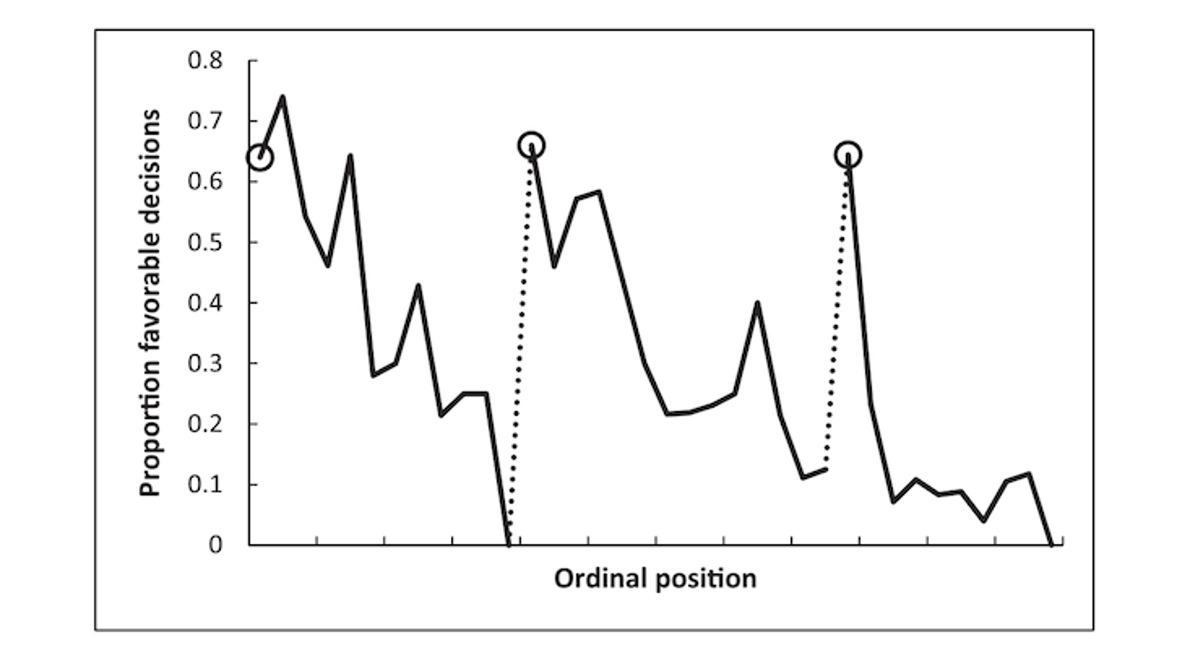
\includegraphics[width=1\linewidth]{images/hungryjudges} 

}

\caption{Proportion of rulings in favor of the prisoners by ordinal position. Circled points indicate the first decision in each of the three decision sessions; tick marks on x axis denote every third case; dotted line denotes food break. From Danziger, S., Levav, J., & Avnaim-Pesso, L. (2011). Extraneous factors in judicial decisions. Proceedings of the National Academy of Sciences, 108(17), 6889–6892. https://doi.org/10.1073/PNAS.1018033108}\label{fig:hungryjudges}
\end{figure}

We see a graphical representation of the proportion of favorable parole decisions that real-life judges are making as a function of the number of cases they process across the day in Figure @ref\{fig:hungryjudges\}). This study is mentioned in many popular science books as an example of a finding that shows that people do not always make rational decisions, but that ``judicial rulings can be swayed by extraneous variables that should have no bearing on legal decisions'' \citep{danziger_extraneous_2011}. We see that early on in the day, judges start by giving about 65\% of people parole, which basically means, ``All right, you can go back into society.'' But then very quickly, the number of favorable decisions decreases to basically zero. After a quick break which, as the authors say, ``may replenish mental resources by providing rest, improving mood, or by increasing glucose levels in the body'' the parole decisions are back up at 65\%, and then again quickly drop down to basically zero. They take another break, the percentage of positive decisions is back up to 65\%, only to drop again over the course of the day.

If we calculate the effect size for the drop after a break, and before the next break \citep{glockner_irrational_2016}, the effect represents a Cohen's d of approximately two, which is incredibly large. There are hardly any effects in psychology this large, let along effects of mood or rest on decision making. And this surprisingly large effect occurs not just once, but three times over the course of the day. If mental depletion actually has such a huge real-life impact, society would basically fall into complete chaos just before lunch break every day. Or at the very least, our society would have organized itself around this incredibly strong effect of mental depletion. Just like manufacturers take size differences between men and women into account when producing items such as golf clubs or watches, we would stop teaching in the time before lunch, doctors would not schedule surgery, and driving before lunch would be illegal. If a psychological effect is this big, we don't need to discover it and publish it in a scientific journal - you would already know it exists.

We can look at a meta-meta-analysis (a paper that meta-analyzes a large number of meta-analyses in the literature) by Richard, Bond, \& Stokes-Zoota \citeyearpar{richard_one_2003} to see which effect sizes in law psychology are close to a Cohen's d of 2. They report two meta-analyzed effects that are slightly smaller. The first is the effect that a jury's final verdict is likely to be the verdict a majority initially favored, which 13 studies show has an effect size of r = 0.63, or d = 1.62. The second is that when a jury is initially split on a verdict, its final verdict is likely to be lenient, which 13 studies show to have an effect size of r = .63 as well. In their entire database, some effect sizes that come close to d = 2 are the finding that personality traits are stable over time (r = 0.66, d = 1.76), people who deviate from a group are rejected from that group (r = .6, d = 1.5), or that leaders have charisma (r = .62, d = 1.58). You might notice the almost tautological nature of these effects. And that is, supposedly, the effect size that the passing of time (and subsequently eating lunch) has on parole hearing sentencings.

We see how examining the size of an effect can lead us to identify findings that can not be caused by their proposed mechanisms. The effect reported in the hungry judges study must thefore be due to a confound. Indeed, such confounds have been identified, as it turns out the ordering of the cases is not random, and it is likely the cases that deserve parole are handled first, and the cases that do not deserve parole are handled later \citep{weinshall-margel_overlooked_2011, chatziathanasiou_beware_2022}. A additional use of effect sizes is to identify effect sizes that are too large to be plausible. Hilgard \citeyearpar{hilgard_maximal_2021} proposes to build in `maximum positive controls', experimental conditions that show the largest possible effect that provides an upper limit on plausible effect size measures.

\hypertarget{cohend}{%
\section{Standardised Mean Differences}\label{cohend}}

Effect sizes can be grouped into two families \citep{rosenthal_contrasts_2000}: The \textbf{d family} (based on standardized mean differences) and the \textbf{r family} (based on measures of strength of association). Conceptually, the \emph{d} family effect sizes are based on a comparison between the difference between the observations, divided by the standard deviation of these observations. This means that a Cohen's \emph{d} = 1 means the standardized difference between two groups equals one standard deviation. The size of the effect in the Facebook study above was quantified with Cohen's \emph{d}. Cohen's \emph{d} (the \emph{d} is \href{https://blog.apastyle.org/apastyle/2011/08/the-grammar-of-mathematics-writing-about-variables.html}{italicized}) is used to describe the standardized mean difference of an effect. This value can be used to compare effects across studies, even when the dependent variables are measured with different scales, for example when one study uses 7-point scales to measure dependent variables, while the other study uses 9-point scales. We can even compare effect sizes across completely different measures of the same construct, one study uses a self-report measure, and another study uses a physiological measure. Although we can compare effect sizes across different measurements, this does not mean they are comparable, as we will discuss in more detail in the section on \protect\hyperlink{heterogeneity}{heterogeneity} in the chapter on meta-analysis.

Cohen's \emph{d} ranges from 0 to infinity. Cohen \citeyearpar{cohen_statistical_1988} uses subscripts to distinguish different versions of Cohen's \emph{d}, a practice I will follow because it prevents confusion (without any specification, Cohen's \emph{d} denotes the entire family of effect sizes). Cohen refers to the standardized mean difference between two groups of independent observations for the \emph{sample} as \(d_s\). Before we get into the statistical details, let's first visualize what a Cohen's d of 0.001 (as was found in the Facebook study) means. We will use a vizualization from \url{http://rpsychologist.com/d3/cohend/}, a website made by Kristoffer Magnusson, that allows you to visualize the differences between two measurements (such as the increase in negative words used by the Facebook user when the number of positive words on the timeline was reduced). The vizualization actually shows two distributions, one dark blue and one light blue, but they overlap so much that the tiny difference in distributions is not visible (click the settings button to change the slider settings, and set the step size to 0.001 to reproduce the figure below in the online app).

\begin{figure}

{\centering 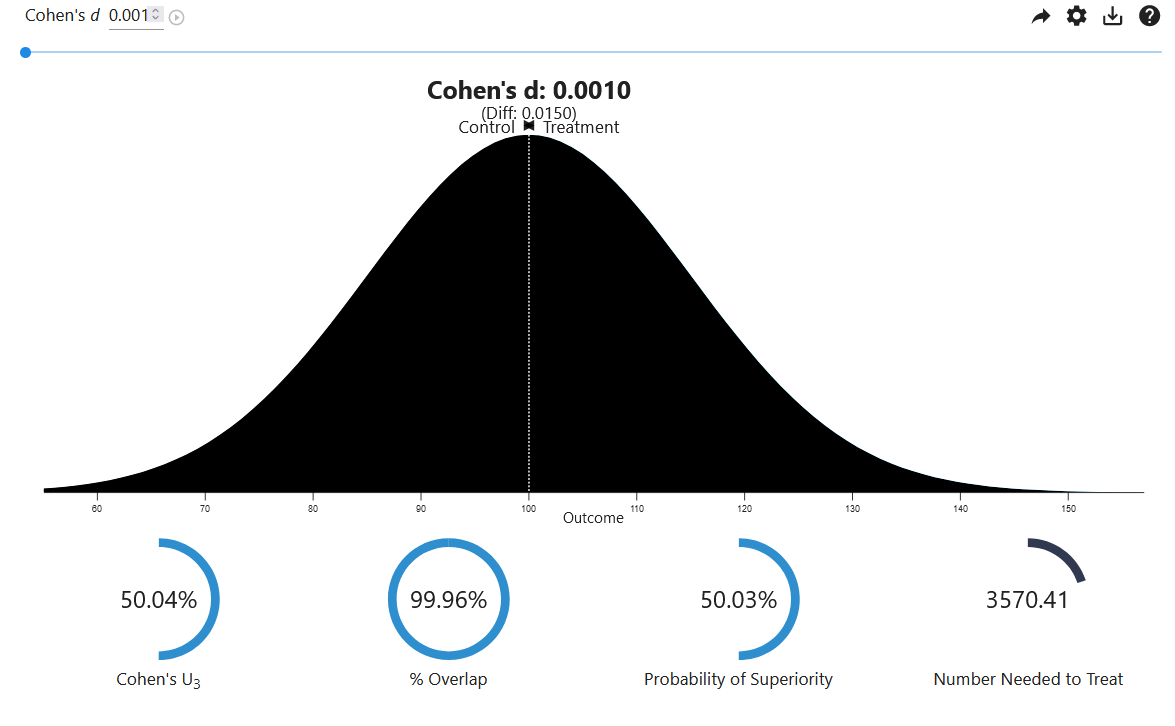
\includegraphics[width=1\linewidth]{images/rpsychd1} 

}

\caption{A vizualization of 2 groups (although the difference is hardly visible) representing d = 0.001.}\label{fig:rpsychd1}
\end{figure}

The four numbers below the distribution express the effect size in different ways to facilitate the interpretation. For example, the probability of superiority expresses the probability that a randomly picked observation from one group will have a larger score than a randomly picked observation from the other group. Because the effect is so small, this probability is 50.03\% - which means that people in the experimental write almost the same number of positive or negative words as people in the control condition. The \emph{number needed to treat} index illustrates that in the Facebook study a person needs to type 3570 words before we will observe one additional negative word, compared to the control condition. I don't know how often you type this many words on Facebook, but I think we can agree this effect is not noticeable on an individual level.

To understand how Cohen's \emph{d} for two independent groups is calculated, let's first look at the formula for the \emph{t}-statistic:

\[
t = \frac{{\overline{M}}_{1}{- \overline{M}}_{2}}{\text{SD}_{\text{pooled}} \times \sqrt{\frac{1}{n_{1}} + \frac{1}{n_{2}}}}
\]

Here \({\overline{M}}_{1}{- \overline{M}}_{2}\) is the difference between the means, and \(\text{SD}_{\text{pooled}}\) is the pooled standard deviation \citep{lakens_calculating_2013}, and n1 and n2 are the sample sizes of the two groups that are being compared. The \emph{t}-value is used to determine whether the difference between two groups in a \emph{t}-test is statistically significant (as eexplained in the chapter on \protect\hyperlink{pvalue}{\emph{p}-values}. The formula for Cohen's \emph{d}\_ is very similar:

\[d_s = \frac{{\overline{M}}_{1}{-\overline{M}}_{2}}{\text{SD}_{\text{pooled}}}\]

As you can see, the sample size in each group (n1 and n2) is part of the formula for a \emph{t}-value, but it is not part of the formula for Cohen's \emph{d} (the pooled standard deviation is computed by weighing the standard deviation in each group by the sample size, but it cancels out if groups are of equal size). This distinction is useful to know, because in practice it means that the \emph{t}-value (and consequently, the \emph{p}-value) is a function of the sample size, but Cohen's \emph{d} is independent of the sample size. If there is a true effect (e.g., a non-zero effect size in the population) the \emph{t}-value for a null-hypothesis test against an effect of zero will on average become larger (and the \emph{p}-value will become smaller) as the sample size increases. The effect size, however, will not increase or decrease, but will become more accurate, as the standard error decreases as the sample size increases. This is also the reason why \emph{p}-values can not be used to make a statement about whether an effect is \emph{practically significant}, and effect size estimates are often such an important complement to \emph{p}-values when making statistical inferences.

You can calculate Cohen's \emph{d} for independent groups from the independent samples \emph{t}-value (which can often be convenient when the result section of the paper you are reading does not report effect sizes) through:

\[d_s = t ⨯ \sqrt{\frac{1}{n_{1}} + \frac{1}{n_{2}}}\]

A d = 001 is an extremely tiny effect, so let's explore an effect size that is a bit more representative of what you would read in the literature. In the meta-meta-analysis mentioned earlier, the median effect size in published studies included in meta-analyses in the psychological literature is \emph{d} = 0.43 \citep{richard_one_2003}. To get a feeling for this effect size, let's use the online app and set the effect size to d = 0.43.

\begin{figure}

{\centering \includegraphics[width=1\linewidth]{images/rpsychd2} 

}

\caption{A vizualization of 2 groups representing d = 0.43.}\label{fig:rpsychd2}
\end{figure}

One example of a meta-analytic effect size in the meta-meta-analysis that is exactly \(d_s\) = 0.43 is the finding that people in a group work less hard to achieve a goal than people who work individually, called \emph{social loafing}. This is an effect that is large enough that we notice it in daily life. Yet, if we look at the overlap in the two distributions, we see that the amount of effort people put in overlaps considerably between the two conditions (in the case of social loafing, working individually versus working in a group). We see in Figure \ref{fig:rpsychd2} that the \textbf{probability of superiority}, or the probability that if we randomly draw one person from the group condition and one person from the individual condition, the person working in a group puts in less effort, is only 61.9\%. This interpretation of differences between groups is also called the \textbf{common language effect size} \citep{mcgraw_common_1992}.

\begin{figure}

{\centering \includegraphics[width=1\linewidth]{images/rpsychd3} 

}

\caption{A vizualization of 2 groups representing d = 2.}\label{fig:rpsychd3}
\end{figure}

Based on \href{http://www.nature.com/pr/journal/v73/n3/full/pr2012189a.html}{this data}, the difference between the height of 21-year old men and women in The Netherlands is approximately 13 centimeters (in an unstandardized effect size), or a standardized effect size of \(d_s\) = 2. If I pick a random man and a random woman walking down the street in my hometown of Rotterdam, how likely is it that the man will be taller than the woman? We see this is quite likely, with a probability of superiority of 92.1\%. But even with such a huge effect, there is still considerable overlap in the two distributions. If we conclude the length of people in one group is larger than the length of people in another group, this does not mean everyone in one group is larger than everyone in the other group.

Sometimes when you try to explain scientific findings at a birthday party, a skeptical aunt or uncle might remark `well I don't believe that is true because \emph{I} never experience this'. With probabilistic observations, there is a distribution of observed effects. In the example about social loafing, on average people put in less effort to achieve a goal when working in a group than working by themselves. For any individual in the population, the effect might be larger, smaller, absent, or even in the opposite direction. If your skeptical aunt or uncle never experience a finding, that does not contradict that the effect is real on average in the population. Indeed, it is even expected that there is no effect for some people in the population, at least some of the time. Although there might be some exceptions (e.g., almost every individual will experience the Stroop effect, where they are slower naming the ink color of color words when the color word is incongruent with the ink it is written in, than when it is congruent with the ink it is written in), but many effects are smaller, or have sufficient variation, that the effect is not present for everyone in the population.

Conceptually, calculating Cohen's \emph{d} for within-subjects comparisons is based on the same idea as for independent groups, where the differences between two observations are divided by the standard deviation within the groups of observations. However, in the case of correlated samples the most common standardizer is the standard deviation of the difference scores. Testing whether two correlated means are significantly different from each other with a paired samples \emph{t}-test is the same as testing whether the difference scores of the correlated means is signicantly different from 0 in a one-sample \emph{t}-test. Similarly, calculating the effect size for the difference between two correlated means is similar to the effect size that is calculated for a one sample \emph{t}-test. The standardized mean difference effect size for within-subjects designs is referred to as Cohen's \(d_z\), where the \emph{z} alludes to the fact that the unit of analysis is no longer \emph{x} or \emph{y}, but their difference, \emph{z}, and can be calculated with:

\[d_z = \frac{M_{dif}}{\sqrt{\frac{\sum{({X_{dif}-M_{dif})}}^2}{N-1}}}\]
The effect size estimate Cohen's dz can also be calculated directly from the t-value and the number of participants using the formula:

\[d_z = \frac{t}{\sqrt{n}}\]

Given the direct relationship between the \emph{t}-value of a paired-samples \emph{t}-test and Cohen's \(d_z\), it will not be surprising that software that performs power analyses for within-subjects designs (e.g., G*Power) relies on Cohen's \(d_z\) as input.

Maxwell \& Delaney \citeyearpar{maxwell_designing_2004} remark: `a major goal of developing effect size measures is to provide a standard metric that meta-analysts and others can interpret across studies that vary in their dependent variables as well as types of designs.' BEcause Cohen's \(d_z\) takes the correlation between the dependent measures into account, it can not be directly compared with Cohen's \(d_s\). Some researchers prefer to use the average standard deviation of both groups of observations as a standardizer (which ignores the correlation between the observations), because this allows for a more direct comparison with Cohen's \(d_s\). This effect size is referred to as Cohen's \(d_av\) \citep{cumming_understanding_2013}, and is simply:

\[d_{av} = \frac{M_{dif}}{\frac{SD_1+SD_2}{2}}\]

\hypertarget{interpreting-effect-sizes}{%
\section{Interpreting effect sizes}\label{interpreting-effect-sizes}}

A commonly used interpretation of Cohen's \emph{d} is to refer to effect sizes as small (\emph{d} = 0.2), medium (\emph{d} = 0.5), and large (\emph{d} = 0.8) based on benchmarks suggested by Cohen (1988). However, these values are arbitrary and should not be used. In practice, you will only see them used in a form of circular reasoning: The effect is small, because it is \emph{d} = 0.2, and \emph{d} = 0.2 is small. We see that using the benchmarks adds nothing, beyond covering up the fact that we did not actually interpret the size of the effect. Furthermore, benchmarks for what is a `medium' and `large' effect do not even correspond between Cohen's d and r (as explained by \citet{mcgrath_when_2006},bsee the `Test Yourself' Q12). Any verbal classification based on benchmarks ignores the fact that any effect can be practically meaningful, such as an intervention that leads to a reliable reduction in suicide rates with an effect size of \emph{d} = 0.1. In other cases, an effect size of \emph{d} = 0.1 might have no consequence at all, for example because such an effect is smaller than the just noticeable difference, and is therefore too small to be noticed by individuals in the real world.

\hypertarget{correlations-and-variance-explained}{%
\section{Correlations and Variance Explained}\label{correlations-and-variance-explained}}

The \emph{r} family effect sizes are based on the proportion of variance that is explained by group membership (e.g., a correlation of \emph{r} = 0.5 indicates 25\% (\emph{r}2) of the variance is explained by the difference between groups). You might remember that \emph{r} is used to refer to a correlation. The correlation of two continuous variables can range from 0 (completely unrelated) to 1 (perfect positive relationship) or -1 (perfect negative relationship). To get a better feel correlations, play the game \href{http://guessthecorrelation.com/}{guess the correlation} where you will see a scatterplot, and have to guess the correlation between the variables (see figure \ref{fig:guesscorrelation}.

\begin{figure}

{\centering \includegraphics[width=1\linewidth]{images/guesscorrelation} 

}

\caption{Screenshot from Guess the Correlation game (the correct answer is r = 0.24).}\label{fig:guesscorrelation}
\end{figure}

The \emph{r} family effect sizes are calculated from the sum of squares (the difference between individual observations and the mean for the group, squared, and summed) for the effect divided by the sums of squares for other factors in the design. Earlier, I mentioned the median effect size in psychology is \(d_s\) = 0.43. However, the authors actually report their results as a correlation, r = 0.21. We can convert Cohen's d into r (but take care that this only applies to \(d_s\), not \(d_z\)):

\[r = \frac{d_s}{\sqrt{{d_s^{2}}^{+}\frac{N^{2} - 2N}{n_{1} \times n_{2}}}}\]

\emph{N} is the total sample size of both groups, whereas n1 and n2 are the sample sizes of the individual groups you are comparing (it is common to use capital N for the total sample size, and lowercase n for sample sizes per group). You can go to \url{http://rpsychologist.com/d3/correlation/} to look at a good visualization of the proportion of variance that is explained by group membership, and the relationship between \emph{r} and \emph{r}2. The amount of variance explained is often quite a small number, and we see in Figure \ref{fig:sharedvariance} that a correlation of 0.21 (the median from the meta-meta-analysis by Richard and colleagues) we see the proportion of variance explained is only 4.4\%. Funder and Ozer \citeyearpar{funder_evaluating_2019} warn against misinterpreting small values for the variance explained as an indication that the effect is not meaningful (and they even consider the practice of squaring the correlation ``actively misleading'').

\begin{figure}

{\centering \includegraphics[width=1\linewidth]{images/sharedvariance} 

}

\caption{Screenshot from correation effect size vizualization by Kristoffer Magnusson for r - 0.21.}\label{fig:sharedvariance}
\end{figure}

As we have seen before, it can be useful to interpret effect sizes to identify effects that are practically insignificant, or effects that are implausibly large. Let's take a look at a study that examines the number of suicides as a function of the amount of country music played on the radio. You can find the paper \href{https://heinonline.org/HOL/P?h=hein.journals/josf71\&i=227}{here} It won an \href{http://www.abc.net.au/science/articles/2004/10/01/1211441.htm}{Ig Nobel prize for studies that first make you laugh, and then think}, although in this case, the the study should not make you think about country music, but about the importance of interpreting effect sizes.

The authors predicted the following:

\begin{quote}
We contend that the themes found in country music-foster a suicidal mood among people already at risk of suicide and that it is thereby associated with a high suicide rate.
\end{quote}

Then they collected data:

\begin{quote}
Our sample is comprised of 49 large metropolitan areas for which data on music were available. Exposure to country music is measured as the proportion of radio airtime devoted to country music. Suicide data were extracted from the annual Mortality Tapes, obtained from the Inter-University Consortium for Political and Social Research (ICPSR) at the University of Michigan. The dependent variable is the number of suicides per 100,000 population.
\end{quote}

And they concluded:

\begin{quote}
A significant zero-order correlation was found between white suicide rates and country music (r = .54, p \textless{} .05). The greater the airtime given to country music, the greater the white suicide rate.
\end{quote}

We can again compare the size of this effects with other known effects in psychology. In the database by Richard and colleagues, there are very few effects this large, but some examples are that leaders are most effective if they have charisma (r = 0.54), good leader--subordinate relations promote subordinate satisfaction (r = 0.53), and people can recognize emotions across cultures (r = 0.53). These effects are all large and obvious, which should raise some doubts about whether the relationship between listening to country music and suicides can be of the same size. Is country music really that bad? If we search the literature, we find that \href{http://sf.oxfordjournals.org/content/74/1/327.short}{other researchers were not able to reproduce the analysis of the original authors}. It is likely that the results are spurious, or a Type 1 error.

Eta squared \(\eta^2\) (part of the \emph{r} family of effect sizes, and an extension of r that can be used for more than two sets of observations) measures the proportion of the variation in Y that is associated with membership of the different groups defined by X, or the sum of squares of the effect divided by the total sum of squares:

\[\eta^{2}$ = $\frac{\text{SS}_{\text{effect}}}{\text{SS}_{\text{total}}}\]

An \(\eta^2\) of .13 means that 13\% of the total variance can be accounted for by group membership. Although \(\eta^2\) is an efficient way to compare the sizes of effects within a study (given that every effect is interpreted in relation to the total variance, all \(\eta^2\) from a single study sum to 100\%), eta squared cannot easily be compared between studies, because the total variability in a study (\(SS_{total}\)) depends on the design of a study, and increases when additional variables are manipulated (e.g., when independent variables are added). Keppel (1991) has recommended partial eta squared (\(\eta_{p}^{2}\)) to improve the comparability
of effect sizes between studies, which expresses the sum of squares of the effect in relation to the sum of squares of the effect and the sum of squares of the error associated with the effect. Partial eta squared is calculated as:

\[\eta_{p}^{2} = \frac{\text{SS}_{\text{effect}}}{\text{SS}_{\text{effect}} + \text{SS}_{\text{error}}}\]

For designs with fixed factors (manipulated factors, or factors that exhaust all levels of the independent variable, such as alive vs.~dead), but not for designs with measured factors or covariates, partial eta squared can be computed from the \emph{F}-value and its degrees of freedom \citep{cohen_statistical_1988}:

\[\eta_{p}^{2} = \frac{F \times \text{df}_{\text{effect}}}{{F \times \text{df}}_{\text{effect}} + \text{df}_{\text{error}}}\]

For example, for an \emph{F}(1, 38) = 7.21, \(\eta_{p}^{2}\) = 7.21 ⨯ 1/(7.21 ⨯ 1 +
38) = 0.16.

Eta squared can be transformed into Cohen's \emph{d}:

\emph{d} = 2\(\times f\) where \(f^{2} = \eta^{2}/(1 - \eta^{2})\)

\hypertarget{correcting-for-bias}{%
\section{Correcting for Bias}\label{correcting-for-bias}}

Population effect sizes are almost always estimated on the basis of samples, and as a measure of the population effect size estimate based on sample averages, Cohen's \emph{d} slighlty overestimates the true population effect. When Cohen's \emph{d} refers to the population, the Greek letter δ is typically used. Therefore, corrections for bias are used (even though these corrections do not always lead to a completely unbiased effect size estimate). In the \emph{d} family of effect sizes, the correction for bias in the population effect size estimate of Cohen's δ is known as Hedges' \emph{g} (although different people use different names -- \(d_{unbiased}\) is also used). This correction for bias is only noticeable in small sample sizes, but since we often use software to calculate effect sizes anyway, it makes sense to always report Hedge's \emph{g} instead of Cohen's \emph{d} \citep{thompson_effect_2007}.

As with Cohen's \emph{d}, \(\eta^2\) is a biased estimate of the true effect size in the population. Two less biased effect size estimates have been proposed, epsilon squared \(\varepsilon^{2}\) and omega squared \(\omega^{2}\). For all practical purposes, these two effect sizes correct for bias equally well \citep{okada_is_2013, albers_when_2018}, and should be preferred above \(\eta^2\). Partial epsilon squared (\(\varepsilon_{p}^{2}\)) and partial omega squared (\(\omega_{p}^{2}\)) can be calculated based on the \emph{F}-value and degrees of freedom.

\[
\omega_{p}^{2} = \frac{F - 1}{F + \ \frac{\text{df}_{\text{error}} + 1}{\text{df}_{\text{effect}}}}
\]

\[
\varepsilon_{p}^{2} = \frac{F - 1}{F + \ \frac{\text{df}_{\text{error}}}{\text{df}_{\text{effect}}}}
\]
Partial effect sizes \(\eta_{p}^{2}\), \(\varepsilon_{p}^{2}\) and \(\omega_{p}^{2}\) can not be generalized across different designs. For this reason, generalized eta-squared (\(\eta_{G}^{2}\)) and generalized omega-squared (\(\omega_{G}^{2}\)) have been proposed \citep{olejnik_generalized_2003}, although they are not very popular. In part, this might be because summarizing the effect size in an ANOVA design with a single index has limitations, and perhaps it makes more sense to describe the pattern of results, as we will see in the section below.

\hypertarget{effect-sizes-for-interactions}{%
\section{Effect Sizes for Interactions}\label{effect-sizes-for-interactions}}

The effect size used for power analyses for ANOVA designs is Cohen's \emph{f}. For two independent groups, Cohen's \(f\) = 0.5 * Cohen's \emph{d}. For more than two groups, Cohen's f can be converted into eta-squared and back with \(f = \frac{\eta^2}{(1 - \eta^2)}\) or \(\eta^2 = \frac{f^2}{(1 + f^2)}\). When predicting interaction effects in ANOVA designs, planning the study based on an expected effect size such as \(\eta_{p}^{2}\) or Cohen's \emph{f} might not be the most intuitive approach.

Let's start with the effect size for a simple two group comparison, and ex effect size to an interaction effect in an ANOVA. Let's assume we predict a mean difference of 1, and know the standard deviation of the measure is 2. This means the standardized effect size is \emph{d} = 0.5. An independent \emph{t}-test is mathematically identical to an \emph{F}-test with two groups. For an \emph{F}-test, the effect size used for power analyses is Cohen's \emph{f}, which is calculated based on the standard deviation of the population means divided by the population standard deviation (which we know for our measure is 2), or:

\begin{equation}
f = \frac{\sigma _{ m }}{\sigma}
\end{equation}
where for equal sample sizes
\begin{equation}
\sigma _{ m } = \sqrt { \frac { \sum_ { i = 1 } ^ { k } ( m _ { i } - m ) ^ { 2 } } { k } }.
\end{equation}

In this formula \emph{m} is the grand mean, k is the number of means, and m\_i is the mean in each group. The formula above might look a bit daunting, but calculating Cohen's f is not that difficult for two groups.

If we take the expected means of 0 and 1, and a standard deviation of 2, the grand mean (the \emph{m} in the formula above) is (0 + 1)/2 = 0.5. The formula says we should subtract this grand mean from the mean of each group, square this value, and sum them. So we have (0-0.5)\^{}2 and (1-0.5)\^{}2, which are both 0.25. We sum these values (0.25 + 0.25 = 0.5), divide them by the number of groups (0.5/2 = 0.25) and take the square root, we find that \(\sigma_{ m }\) = 0.5. We can now calculate Cohen's \emph{f} (using \(\sigma\) = 2 for our measure):

\begin{equation}
f = \frac{\sigma _{ m }}{\sigma} = \frac{0.5}{2} = 0.25
\end{equation}

We confirm that for two groups Cohen's \emph{f} is half as large as Cohen's \emph{d}.

Now we have the basis to look at interaction effects. Different patterns of means in an ANOVA can have the same Cohen's \emph{f}. There are two types of interactions, as visualized below in Figure \ref{fig:interactions}. In an \textbf{ordinal interaction}, the mean of one group (``B1'') is always higher than the mean for the other group (``B2''). \textbf{Disordinal interactions} are also known as `cross-over' interactions, and occur when the group with the larger mean switches over. The difference is important, since the disordinal interaction in Figure \ref{fig:interactions} has a larger effect size than the ordinal interaction.

\begin{figure}

{\centering \includegraphics[width=1\linewidth]{06-effectsize_files/figure-latex/interactions-1} 

}

\caption{Schematic illustration of a disordinal (or cross-over) and ordinal interaction}\label{fig:interactions}
\end{figure}

Mathematically the interaction effect is computed as the cell mean minus the sum of the grand mean, the marginal mean in each condition of one factor minus the grand mean, and the marginal mean in each condition for the other factor minus grand mean \citep{maxwell_designing_2004}.

Let's consider two cases, one where we have a perfect disordinal interaction (the means of 0 and 1 flip around in the other condition, and are 1 and 0) or an ordinal interaction (the effect is present in one condition, with means 0 and 1, but disappears in the other condition, with means 0 and 0, see Figure \ref{fig:interactionplots}).

\begin{figure}

{\centering \includegraphics[width=1\linewidth]{06-effectsize_files/figure-latex/interactionplots-1} 

}

\caption{Disordinal (or cross-over) and ordinal interaction with means of 0 and 1, n = 50 per group, and an sd of 2.}\label{fig:interactionplots}
\end{figure}

We can calculate the interaction effect as follows (we will go through the steps in some detail). First, let's look at the disordinal interaction. The grand mean is (1 + 0 + 0 + 1) / 4 = 0.5.

We can compute the marginal means for A1, A2, B1, and B2, which is simply averaging per row and column, which gets us for the A1 row (1+0)/2=0.5. For this perfect disordinal interaction, all marginal means are 0.5. This means there are no main effects. There is no main effect of factor A (because the marginal means for A1 and A2 are both exactly 0.5), nor is there a main effect of B.

We can also calculate the interaction effect. For each cell we take the value in the cell (e.g., for a1b1 this is 1) and compute the difference between the cell mean and the additive effect of the two factors as:

1 - (the grand mean of 0.5 + (the marginal mean of a1 minus the grand mean, or 0.5 - 0.5 = 0) + (the marginal mean of b1 minus the grand mean, or 0.5 - 0.5 = 0)). Thus, for each cell we get:

a1b1: 1 - (0.5 + (0.5 -0.5) + (0.5 -0.5)) = 0.5

a1b2: 0 - (0.5 + (0.5 -0.5) + (0.5 -0.5)) = -0.5

a2b1: 0 - (0.5 + (0.5 -0.5) + (0.5 -0.5)) = -0.5

a2b2: 1 - (0.5 + (0.5 -0.5) + (0.5 -0.5)) = 0.5

Cohen's \(f\) is then \(f = \frac { \sqrt { \frac { 0.5^2 +-0.5^2 + -0.5^2 + 0.5^2 } { 4 } }}{ 2 } = 0.25\)

For the ordinal interaction the grand mean is (1 + 0 + 0 + 0) / 4, or 0.25. The marginal means are a1: 0.5, a2: 0, b1: 0.5, and b2: 0.

Completing the calculation for all four cells for the ordinal interaction gives:

a1b1: 1 - (0.25 + (0.5 -0.25) + (0.5 -0.25)) = 0.25

a1b2: 0 - (0.25 + (0.5 -0.25) + (0.0 -0.25)) = -0.25

a2b1: 0 - (0.25 + (0.0 -0.25) + (0.5 -0.25)) = -0.25

a2b2: 0 - (0.25 + (0.0 -0.25) + (0.0 -0.25)) = 0.25

Cohen's \(f\) is then \(f = \frac { \sqrt { \frac { 0.25^2 +-0.25^2 + -0.25^2 + 0.25^2 } { 4 } }}{ 2 } = 0.125\).

We see the effect size of the cross-over interaction (\emph{f} = 0.25) is twice as large as the effect size of the ordinal interaction (\emph{f} = 0.125). This should make sense if we think about the interaction as a test of contrasts. In the disordinal interaction we are comparing cells a1b1 and a2b2 against a1b2 and a2b1, or (1+1)/2 vs.~(0+0)/2. Thus, if we see this as a \emph{t}-test for a contrast, we see the mean difference is 1. For the ordinal interaction, we have (1+0)/2 vs.~(0+0)/2, so the mean difference is halved, namely 0.5. This obviously matters for the statistical power we will have when we examine interaction effects in our experiments.

Just stating that you expect a `medium' Cohen's \emph{f} effect size for an interaction effect in your power analysis is not the best approach. Instead, start by thinking about the pattern of means and standard deviations (and for within factors, the correlation between dependent variables) and then compute the effect size from the data pattern. If you prefer not to do so by hand, you can use \href{https://aaroncaldwell.us/SuperpowerBook/}{Superpower} \citep{lakens_simulation-based_2021}. This also holds for more complex designs, such as multilevel models. In these cases, it is often the case that power analyses are easier based on simulation-based approaches, than based on plugging in a single effect size in power analysis software \citep{debruine_understanding_2021}.

\hypertarget{test-yourself-4}{%
\section{Test Yourself}\label{test-yourself-4}}

\textbf{Q1}: One of the largest effect sizes in the meta-meta analysis by Richard and colleagues from 2003 is that people are likely to perform an action if they feel positively about the action and believe it is common. Such an effect is (with all respect to all researchers who contributed research to this meta-analysis) somewhat trivial. Even so, the correlation was \emph{r} = .66, which equals a Cohen's \emph{d} of 1.76. What is according to the online app at \url{https://rpsychologist.com/cohend/} the probability of superiority for an effect of this size?

\begin{enumerate}
\def\labelenumi{\Alph{enumi})}
\tightlist
\item
  70.45\%
\item
  88.12\%
\item
  89.33\%
\item
  92.14\%
\end{enumerate}

\textbf{Q2}: Cohen's \emph{d} is to \_\_\_\_\_\_ as eta-squared is to \_\_\_\_\_\_\_\_

\begin{enumerate}
\def\labelenumi{\Alph{enumi})}
\tightlist
\item
  r; epsilon-squared
\item
  Hedges' g; omega-squared
\item
  Cohen's d\_s; generalized eta-squared
\end{enumerate}

\textbf{Q3}: A correlation of \emph{r} = 1.2 is:

\begin{enumerate}
\def\labelenumi{\Alph{enumi})}
\tightlist
\item
  Impossible
\item
  Implausibly large for an effect size in the social sciences
\item
  In line with the median effect size in psychology
\end{enumerate}

\textbf{Q4}: Let's assume the difference between two means we observe is 1, and the pooled standard deviation is also 1. What, on average, happens to the \emph{t}-value and Cohen's \emph{d}, as we would simulate studies, as a function of the sample size in these simulations?

\begin{enumerate}
\def\labelenumi{\Alph{enumi})}
\tightlist
\item
  Given the mean difference and standard deviation, as the sample size becomes bigger, the \emph{t}-value become larger, and Cohen's \emph{d} becomes larger.
\item
  Given the mean difference and standard deviation, as the sample size becomes bigger, the \emph{t}-value gets closer to the true value, and Cohen's \emph{d} becomes larger.
\item
  Given the mean difference and standard deviation, as the sample size becomes bigger, the \emph{t}-value become larger, and Cohen's \emph{d} gets closer to the true value.
\item
  Given the mean difference and standard deviation, as the sample size becomes bigger, the \emph{t}-value gets closer to the true value, and Cohen's \emph{d} gets closer to the true value.
\end{enumerate}

\textbf{Q5}: Go to \url{http://rpsychologist.com/d3/correlation/} to look at a good visualization of the proportion of variance that is explained by group membership, and the relationship between \emph{r} and \emph{r}2. Look at the scatterplot and the shared variance for an effect size of \emph{r} = .21 (Richard, Bond, \& Stookes-Zoota, 2003).Given that \emph{r} = 0.21 was the average effect size in psychological research, how much variance in the data do we on average explain?

\begin{enumerate}
\def\labelenumi{\Alph{enumi})}
\tightlist
\item
  2.1\%
\item
  21\%
\item
  4.4\%
\item
  44\%
\end{enumerate}

\textbf{Q6}: By default, the sample size for the online correlation visualization linked to above is 50. Click on the cogwheel to access the settings, and change it to 500. What happens?

\begin{enumerate}
\def\labelenumi{\Alph{enumi})}
\tightlist
\item
  The proportion of explained variance is 5 times as large.
\item
  The proportion of explained variance is 5 times as small.
\item
  The proportion of explained variance is 52 times as large.
\item
  The proportion of explained variance stays the same.
\end{enumerate}

\textbf{Q7}: In an old paper you find a statistical result reported as \emph{t}(36) = 2.14 \emph{p} \textless{} 0.05 for an independent \emph{t}-test without a reported effect size. Using the online MOTE app \url{https://doomlab.shinyapps.io/mote/} (choose Independent t -t from the Mean Differences dropdown menu) or the MOTE R function d.ind.t.t, what is the effect size Cohen's \emph{d} for this effect, given 38 participants (e.g., 18 in each group, leading to N -- 2 = 36 degrees of freedom) and an alpha level of 0.05?

\begin{enumerate}
\def\labelenumi{\Alph{enumi})}
\tightlist
\item
  d = 0.38
\item
  d = 0.41
\item
  d = 0.71
\item
  d = 0.75
\end{enumerate}

\textbf{Q8}: In an old paper you find a statistical result from a 2x3 between subjects ANOVA reported as \emph{F}(2, 122) = 4.13, \emph{p} \textless{} 0.05, without a reported effect size. Using the online MOTE app \url{https://doomlab.shinyapps.io/mote/} (choose Eta -- F from the Variance Overlap dropdown menu) or the MOTE R function eta.F, what is the effect size in partial eta-squared?

\begin{enumerate}
\def\labelenumi{\Alph{enumi})}
\tightlist
\item
  \(\eta_p^2\) = 0.063
\item
  \(\eta_p^2\) = 0.996
\item
  \(\eta_p^2\) = 0.032
\item
  \(\eta_p^2\) = 0.049
\end{enumerate}

\textbf{Q9}: You realize that computing omega-squared corrects for some of the bias in eta-squared. For the old paper with \emph{F}(2, 122) = 4.13, \emph{p} \textless{} 0.05, and using the online MOTE app \url{https://doomlab.shinyapps.io/mote/} (choose Omega -- F from the Variance Overlap dropdown menu) or the MOTE R function omega.F, what is the effect size in partial omega-squared? HINT: The total sample size is the df error + k, where k is the number of groups (which is 6 for the 2x3 ANOVA).

\begin{enumerate}
\def\labelenumi{\Alph{enumi})}
\tightlist
\item
  \(\eta_p^2\) = 0.047
\item
  \(\eta_p^2\) = 0.749
\item
  \(\eta_p^2\) = 0.032
\item
  \(\eta_p^2\) = 0.024
\end{enumerate}

\textbf{Q10}: Several times in this chapter the effect size Cohen's d was converted to r, or vice versa. We can use the \texttt{effectsize} R package (that can also be used to compute effect sizes when you analyze your data in R) to convert the median r = 0.21 observed in Richard and colleagues' meta-meta-analysis to d: effectsize::r\_to\_d(0.21) which yields d = 0.43 (the conversion assumes equal sample sizes in each group). Which Cohen's \emph{d} corresponds to a \emph{r} = 0.1?

\begin{enumerate}
\def\labelenumi{\Alph{enumi})}
\tightlist
\item
  d = 0.05
\item
  d = 0.10
\item
  d = 0.20
\item
  d = 0.30
\end{enumerate}

\textbf{Q11}: It can be useful to convert effect sizes to r when performing a meta-analysis where not all effect sizes that are included are based on mean differences. Using the d\_to\_r function in the \texttt{effectsize} package, what does a \emph{d} = 0.8 correspond to?

\begin{enumerate}
\def\labelenumi{\Alph{enumi})}
\tightlist
\item
  r = 0.30
\item
  r = 0.37
\item
  r = 0.50
\item
  r = 0.57
\end{enumerate}

\textbf{Q12}: From questions 10 and 11 you might have noticed something peculiar. The benchmarks typically used for `small', `medium', and `large' effects for Cohen's d are \emph{d} = 0.2, \emph{d} = 0.5, and \emph{d} = 0.8, and for a correlation are \emph{r} = 0.1, \emph{r} = 0.3, and \emph{r} = 0.5. Using the d\_to\_r function in the \texttt{effectsize} package, check to see whether the benchmark for a `large' effect size correspond between \emph{d} and \emph{r}.

As \citet{mcgrath_when_2006} write: ``Many users of Cohen's (1988) benchmarks seem unaware that those for the correlation coefficient and d are not strictly equivalent, because Cohen's generally cited benchmarks for the correlation were intended for the infrequently used biserial correlation rather than for the point biserial.''

Download the paper by McGrath and Meyer, 2006 (you can find links to the pdf \href{https://scholar.google.com/scholar?cluster=18022919125620514097\&as_sdt=0\%2C5\&inst=1903264034810781805}{here}), and on page 390, right column, read which solution the authors prefer.

\begin{enumerate}
\def\labelenumi{\Alph{enumi})}
\tightlist
\item
  Just stop using these silly benchmarks.
\item
  No, honestly, just really stop using these silly benchmarks.
\item
  The benchmarks for \emph{d} would need to be changed to 0.20, 0.67, and 1.15
\item
  The benchmarks for correlations would need to be changed to .10, .24, and .37
\end{enumerate}

\hypertarget{confint}{%
\chapter{Confidence Intervals}\label{confint}}

When we report point estimates, we should acknowledge and quantify the uncertainty in these estimates. Confidence intervals provide a way to quantify the precision of an estimate. By reporting an estimate with a confidence interval, results are reported within a range of value that contain the true value of the parameter with a desired percentage. For example, when we report an effect size estimate with a 95\% confidence interval, the expectation is that the interval is wide enough such that 95\% of the time the range of values around the estimate contains the true parameter value.

\hypertarget{population-vs.-sample}{%
\section{Population vs.~Sample}\label{population-vs.-sample}}

In statistics, we differentiate between the population and the sample. The population is everyone you are interested in, such as all people in the world, elderly who are depressed, or people who buy innovative products. Your sample is everyone you were able to measure from the population you are interested in. We similarly distinguish between a parameter and a statistic. A parameter is a characteristic of the population, while a statistic is a characteristic of a sample. Sometimes, you have data about your entire population. For example, we have measured the height of all the people who have ever walked on the moon. We can calculate the average height of these twelve individuals, and so we know the true parameter. We do not need inferential statistics. However, we do not know the average height of all people who have ever walked on the earth. Therefore, we need to estimate this parameter, using a statistic based on a sample. Although it is rare that a study includes the entire population, it is not impossible, as illustrated in Figure \ref{fig:population}.

\begin{figure}

{\centering \includegraphics[width=1\linewidth]{images/population} 

}

\caption{Example of a registry-based study in which the entire population was included in the study. From https://doi.org/10.1093/ije/dyab066}\label{fig:population}
\end{figure}

When the entire population is measured there is no need to perform a hypothesis test. After all, there is no population to generalize to (although it is possible to argue we are still making an inference, even when the entire population is observed, because we have observed a \emph{metaphorical population} from one of many possible worlds, see \citet{spiegelhalter_art_2019}). When data from the entire population has been collected the population effect size is known, and there is no confidence interval to compute. If the total population size is known, but not measured completely, then the confidence interval width should shrink to zero the closer a study gets to measuring the entire population. This is known as the finite population correction factor for the variance of the estimator \citep{kish_survey_1965}. The variance of a sample mean is \(\sigma^2/n\), which for finite populations is multiplied by the finite population correction factor of the standard error:
\[FPC = \sqrt{\frac{(N - n)}{(N-1)}}\]
where \emph{N} is the size of the population, and \emph{n} is the size of the sample. When \emph{N} is much larger than \emph{n}, the correction factor will be close to 1 (and therefore this correction is typically ignored when populations are very large, even when populations are finite), and will not have a noticeable effect on the variance. When the total population is measured the correction factor is 0, such that the variance becomes 0 as well. For example, when the total population consists of 100 top athletes, and data is collected from a sample of 35 athletes, the finite population correction is \(\sqrt{(100 - 35)/(100-1)}\) = 0.81. The \texttt{superb} R package can compute population corrected confidence intervals \citep{cousineau_superb_2019}.

\hypertarget{what-is-a-confidence-interval}{%
\section{What is a Confidence Interval?}\label{what-is-a-confidence-interval}}

Confidence intervals are a statement about the percentage of confidence intervals that contain the true parameter value. This behavior of confidence intervals is nicely visualized on this website by Kristoffer Magnusson: \url{http://rpsychologist.com/d3/CI/}. In Figure \ref{fig:cisim} We see blue dots that represent means from a sample, and that fall around a red vertical line, which represents the true value of the parameter in the population. Due to variation in the sample, the estimates do not all fall on the red line. The horizontal lines around the blue dots are the confidence intervals. By default, the visualization shows 95\% confidence intervals. Most of the lines are black (which means the confidence interval overlaps with the red line indication the true population value), but some are red (indicating they do not capture the true population value). In the long run, 95\% of the horizontal bars will be black, and 5\% will be red.

\begin{figure}

{\centering \includegraphics[width=1\linewidth]{images/cisim} 

}

\caption{Series of simulated point estimates and confidence intervals}\label{fig:cisim}
\end{figure}

We can now see what is meant by the sentence ``Confidence intervals are a statement about the percentage of confidence intervals that contain the true parameter value``. In the long run, for 95\% of the samples, the red line (the population parameter) is contained within the 95\% confidence interval around the sample mean, and in 5\% of the confidence intervals this is not true. As we will see when we turn to the formula for confidence intervals, the width of a confidence interval depends on the sample size and the standard deviation. The larger the sample size, the smaller the confidence intervals.

\hypertarget{relatCIp}{%
\section{\texorpdfstring{The relation between confidence intervals and \emph{p}-values}{The relation between confidence intervals and p-values}}\label{relatCIp}}

There is a direct relationship between the CI around an effect size and statistical significance of a null-hypothesis significance test. For example, if an effect is statistically significant (\emph{p} \textless{} 0.05) in a two-sided independent \emph{t}-test with an alpha of .05, the 95\% CI for the mean difference between the two groups will not include zero. Confidence intervals are sometimes said to be more informative than \emph{p}-values, because they do not only provide information about whether an effect is statistically significant (i.e., when the confidence interval does not overlap with the value representing the null hypothesis), but also communicate the precision of the effect size estimate. This is true, but as mentioned in the chapter on \href{pvalue}{\emph{p}-values} it is still recommended to add exact \emph{p}-values, which facilitates the re-use of results for secondary analyses \citep{appelbaum_journal_2018}, and allows other researchers to compare the \emph{p}-value to an alpha level they would have preferred to use \citep{lehmann_testing_2005}.

In order to maintain the direct relationship between a confidence interval and a \emph{p}-value it is necessary to adjust the confidence interval level whenever the alpha level is adjusted. For example, if an alpha level of 5\% is corrected for three comparisons to 0.05/3 - 0.0167, the corresponding confidence interval would be a 1 - 0.0167 = 0.9833 confidence interval. Similarly, if a \emph{p}-value is computed for a one-sided \emph{t}-test, there is only an upper or lower limit of the interval, and the other end of the interval ranges to −∞ or ∞.

To maintain a direct relationship between an \emph{F}-test and its confidence interval, a 90\% CI for effect sizes from an \emph{F}-test should be provided. The reason for this is explained by \href{http://core.ecu.edu/psyc/wuenschk/docs30/CI-Eta2-Alpha.doc}{Karl Wuensch}. Where Cohen's d can take both positive and negative values, r² or η² are squared, and can therefore only take positive values. This is related to the fact that \emph{F}-tests (as commonly used in ANOVA) are one-sided. If you calculate a 95\% CI, you can get situations where the confidence interval includes 0, but the test reveals a statistical difference with a \emph{p} \textless{} .05 (for a more mathematical explanation, see \citet{steiger_beyond_2004}). This means that a 95\% CI around Cohen's d in an independent \emph{t}test equals a 90\% CI around η² for exactly the same test performed as an ANOVA. As a final detail, because eta-squared cannot be smaller than zero, the lower bound for the confidence interval can not be smaller than 0. This means that a confidence interval for an effect that is not statistically different from 0 has to start at 0. You report such a CI as 90\% CI {[}.00; .XX{]} where the XX is the upper limit of the CI.

Confidence intervals are often used in forest plots that communicate the results from a meta-analysis. In the plot below, we see 4 rows. Each row shows the effect size estimate from one study (in Hedges' g). For example, study 1 yielded an effect size estimate of 0.44, with a confidence interval around the effect size from 0.08 to 0.8. The horizontal black line, similarly to the visualization we played around with before, is the width of the confidence interval. When it does not touch the effect size 0 (indicated by a black vertical line) the effect is statistically significant.

\begin{figure}

{\centering \includegraphics[width=1\linewidth]{07-CI_files/figure-latex/meta-1} 

}

\caption{Meta-analysis of 4 studies}\label{fig:meta}
\end{figure}

We can see, based on the fact that the confidence intervals do not overlap with 0, that studies 1 and 3 were statistically significant. The diamond shape next the FE model (Fixed Effect model) is the meta-analytic effect size. Instead of using a black horizontal line, the upper limit and lower limit of the confidence interval are indicated by the left and right points of the diamond, and the center of the diamond is the meta-analytic effect size estimate. A meta-analysis calculates the effect size by combining and weighing all studies. The confidence interval for a meta-analytic effect size estimate is always narrower than that for a single study, because of the combined sample size of all studies included in the meta-analysis.

In the preceding section, we focused on examining whether the confidence interval overlapped with 0. This is a confidence interval approach to a null-hypothesis significance test. Even though we are not computing a \emph{p}-value, we can directly see from the confidence interval whether \emph{p} \textless{} \(\alpha\). The confidence interval approach to hypothesis testing makes it quite intuitive to think about performing tests against non-zero null hypotheses \citep{bauer_unifying_1996}. For example, we could test whether we can reject an effect of 0.5 by examining if the 95\% confidence interval does not overlap with 0.5. We can test whether an effect is \emph{smaller} that 0.5 by examining if the 95\% confidence interval falls completely \emph{below} 0.5. We will see that this is leads to a logical extension of null-hypothesis testing where, instead of testing to reject an effect of 0, we can test whether we can reject other effects of interest in \textbf{range predictions} and \protect\hyperlink{equivalencetest}{\textbf{equivalence tests}}.

\hypertarget{the-standard-error-and-95-confidence-intervals}{%
\section{The Standard Error and 95\% Confidence Intervals}\label{the-standard-error-and-95-confidence-intervals}}

To calculate a confidence interval, we need the standard error. The standard error (SE) estimates the variability between sample means that would be obtained after taking several measurements from the same population. It is easy to confuse it with the standard deviation, which is the degree to which individuals within the sample differ from the sample mean. Formally, statisticians distinguish between σ and \(\widehat{\sigma}\), where the hat means the value is estimated from a sample, and the lack of a hat means it is the population value -- but I'll leave out the hat, even when I'll mostly talk about estimated values based on a sample in the formulas below. Mathematically (where σ is the standard
deviation),

\[
Standard \ Error \ (SE) = \sigma/\sqrt n
\]

The standard error of the sample will tend to zero with increasing sample size, because the estimate of the population mean will become more and more accurate. The standard deviation of the sample will become more and more similar to the population standard deviation as the sample size increases, but it will not become smaller. Where the standard deviation is a statistic that is descriptive of your sample, the standard error describes bounds on a random sampling process.

The Standard Error is used to construct confidence intervals (CI) around sample estimates, such as the mean, or differences between means, or whatever statistics you might be interested in. To calculate a confidence interval around a mean (indicated by the Greek letter mu: μ), we use the \emph{t} distribution with the corresponding degrees of freedom (\emph{df} : in a one-sample \emph{t}-test, the degrees of freedom are n-1):

\[
\mu \pm t_{df, 1-(\alpha/2)} SE
\]

With a 95\% confidence interval, the α = 0.05, and thus the critical \emph{t}-value for the degrees of freedom for 1- α /2, or the 0.975th quantile is calculated. Remember that a \emph{t}-distribution has slightly thicker tails than a Z-distribution. Where the 0.975th quantile for a Z-distribution is 1.96, the value for a \emph{t}-distribution with for example df = 19 is 2.093. This value is multiplied by the standard error, and added (for the upper limit of the confidence interval) or subtracted (for the lower limit of the confidence interval) from the mean.

\hypertarget{overlapping-confidence-intervals}{%
\section{Overlapping Confidence Intervals}\label{overlapping-confidence-intervals}}

Confidence intervals are often used in plots. In Figure \ref{fig:cioverlap} below, three estimates are vizluaized (the dots), surrounded by three lines (the 95\% confidence intervals). The left two dots (X and Y) represent the \emph{means} of the independent groups X and Y on a scale from 0 to 8 (see the axis from 0-8 on the left side of the plot). The dotted lines between the two confidence intervals visualize the overlap between the confidence intervals around the means. The two confidence intervals around means in columns X and Y are commonly shown in a figure in a scientific article. The third dot, slightly larger, is the \emph{mean difference} between X and Y, and slightly thicker line visualizes the confidence interval of this mean difference. The difference score is expressed using the axis on the right (from -3 to 5). In the plot below, the mean of group X is 3, the mean of group Y is 5.6, and the difference is 2.6. The plot is based on 50 observations per group, and the confidence interval around the mean difference ranges from 0.49 to 4.68, which is quite wide.

\textbackslash begin\{figure\}

\{\centering \includegraphics[width=1\linewidth]{07-CI_files/figure-latex/cioverlap-1}

\}

\textbackslash caption\{Means and 95\% confidence intervals of two independent groups and the mean difference and it's 95\% confidence interval.\}\label{fig:cioverlap}
\textbackslash end\{figure\}

As mentioned earlier, when a 95\% confidence interval does not contain 0, the effect is statistically different from 0. In Figure \ref{fig:cioverlap} above the mean difference and the 95\% confidence interval around it are indicaed by the `difference' label. As the 95\% confidence interval does not contain 0, the \emph{t}-test is significant at an alpha of 0.05. The \emph{p}-value is indicated in the plot as 0.016. Even though the two means differ statistically from each other, the confidence interval around each mean overlap. One might intuitively believe that an effect is only statistically significant if the confidence interval around the individual means do not overlap, but this is not true. The significance test is related to the confidence interval around the mean difference.

\hypertarget{prediction-intervals}{%
\section{Prediction Intervals}\label{prediction-intervals}}

Even though 95\% of future confidence intervals will contain the true parameter, a 95\% confidence interval will not contain 95\% of future individual observations. Sometimes, researchers want to predict the interval within which a single value will fall. This is called the prediction interval. It is always much wider than a confidence interval. The reason is that individual observations can vary substantially, but means of future samples (which fall within a normal confidence interval 95\% of the time) will vary much less.

In Figure \ref{fig:predictioninterval} the orange background illustrates the 95\% confidence interval around the mean, and the lighter yellow background illustrates the 95\% prediction interval (PI).

\textbackslash begin\{figure\}

\{\centering \includegraphics[width=1\linewidth]{07-CI_files/figure-latex/predictioninterval-1}

\}

\textbackslash caption\{A comparison of a 95\% confidence interval (gold) and 95\% prediction interval (yellow).\}\label{fig:predictioninterval}
\textbackslash end\{figure\}

To calculate the prediction interval, we need a slightly different formula for the standard error, that was used for the confidence interval, namely:

\[
Standard \ Error \ (SE) = \sigma/\sqrt(1+1/n)
\]

When we rewrite the formula used for the confidence interval to \(\sigma/\sqrt(1/N)\), we see the difference between a confidence interval and the prediction interval is in the ``1+'' which always leads to wider intervals. Prediction intervals are \textbf{wider}, because they are constructed so that they will contain \textbf{a single future value} 95\% of the time, instead of the \textbf{mean}. The fact that prediction intervals are wide is a good reminder that it is difficult te predict what will happen for any single individual.

\hypertarget{capture-percentages}{%
\section{Capture Percentages}\label{capture-percentages}}

It can be difficult to understand why a 95\% confidence interval does not provide us with the interval where 95\% of future means will fall. The percentage of means that falls within a single confidence interval is called the \textbf{capture percentage}. In Figure \ref{fig:metaci} we see two randomly simulated studies with the same sample size from the same population. The true effect size in both studies is 0, and we see that the 95\% confidence intervals for both studies contain the true population value of 0. However, the two confidence intervals cover quite different ranges of effect sizes, with the confidence interval in Study 1 ranging from -0.07 to 0.48, and the confidence interval in Study 2 ranging from -0.50 to 0.06. It can not be true that in the future, 95\% of the effect sizes we should expect will fall between -0.07 to 0.048, \textbf{and} 95\% of the effect sizes we should expect will fall between -0.50 to 0.06.

\begin{figure}

{\centering \includegraphics[width=1\linewidth]{07-CI_files/figure-latex/metaci-1} 

}

\caption{Meta-analysis of 2 simulated studies from the same population.}\label{fig:metaci}
\end{figure}

The only situation in which a 95\% confidence interval happens to also be a 95\% capture percentage is when the observed effect size in a sample happens to be exactly the same as the true population parameter. In Figure \ref{fig:metaci} that means we would need to observe an effect of exactly 0. However, you can't know whether your observed effect size happens to be exactly the same as the population effect size. When a sample estimate is not identical to the true population value (which is alsmost always the case) less than 95\% of future effect sizes will fall within the CI from your current sample. As we have observed two studies with observed effect sizes a bit removed from the true effect size, we will find effect size estimates in future studies that fall outside the observed 95\% confidence interval quite often. So, the percentage of future means that fall within a single confidence interval depends upon which single confidence interval you happened to observe. Based on simulation studies it is possible to show that on average, in the long run, a 95\% CI has an 83.4\% capture probability \citep{cumming_confidence_2006}.

\hypertarget{calculating-confidence-intervals-around-standard-deviations.}{%
\section{Calculating Confidence Intervals around Standard Deviations.}\label{calculating-confidence-intervals-around-standard-deviations.}}

If we calculate a standard deviation (SD) from a sample, this value is an
estimate of the true value in the population. In small samples, our estimate can be quite far off. But due to the law of large numbers, as our sample size increases, we will be measuring the standard deviation more accurately. Since the sample standard deviation is an estimate with uncertainty, we can calculate a 95\% confidence interval around it.

Keeping the uncertainty in our estimate of the standard deviation in mind can be important. When researchers perform an a-priori power analysis based on an effect size of interest expressed on a raw scale, they need accurate estimates of the standard deviation when performing the power analysis. Sometimes researchers will use pilot data to get an estimate of the standard deviation. Since the estimate of the population standard deviation based on a pilot study has some uncertainty, the sample size from the a-priori power analysis contains uncertainty (see the `Test Yourself' questions below). Use validated or existing measures for which accurate estimates of the standard deviation in your population of interest are available. And keep in mind that all estimates from a sample have uncertainty.

\hypertarget{computing-confidence-intervals-around-effect-sizes}{%
\section{Computing Confidence Intervals around Effect Sizes}\label{computing-confidence-intervals-around-effect-sizes}}

Cohen \citeyearpar{cohen_earth_1994} reflected on the reason confidence intervals were rarely reporting in 1994: ``I suspect that the main reason they are not reported is that they are so embarrassingly large!'' This might be, but another reason might have been that statistical software rarely provided confidence intervals around effect sizes in the time when Cohen wrote his article. It has become increasingly easy to report confidence intervals with the popularity of free software packages in R, even though these packages might not provide solutions for all statistical tests yet. The \href{https://apastyle.apa.org/jars/quantitative}{Journal Article Reporting Standards} recommend to report ``effect-size estimates and confidence intervals on estimates that correspond to each inferential test conducted, when possible''.

One easy solution to calculating effect sizes and confidence intervals is \href{https://www.aggieerin.com/shiny-server/}{MOTE} made by Dr.~Erin Buchanan and her lab. The website comes with a full collections of tutorials, comparisons with other software packages, and demonstration videos giving accessible overviews of how to compute effect sizes and confidence intervals for a wide range of tests based on summary statistics. This means that whichever software you use to perform statistical tests, you can enter sample sizes and means, standard deviations, or test statistics to compute effect sizes and their confidence intervals. For example, the video below gives an overview of how to compute a confidence interval around Cohen's d for an independent \emph{t}-test.

MOTE is also available as an R package \citep{buchanan_mote_2017}. Although many solutions exists to compute Cohen's d, MOTE sets itself apart by allowing researchers to compute effect sizes and confidence intervals for many additional effect sizes, such as (partial) omega squared for between subjects ANOVA (\(\omega^{2}\) and \(\omega^{2}_p\)), generalized omega squared for ANOVA (\(\omega^{2}_G\)), epsilon squared for ANOVA (\(\varepsilon^{2}\)) and (partial) generalized eta squared for ANOVA (\(\eta^{2}_G\)).

\begin{Shaded}
\begin{Highlighting}[]
\NormalTok{MOTE}\SpecialCharTok{::}\FunctionTok{d.ind.t}\NormalTok{(}\AttributeTok{m1 =} \FloatTok{1.7}\NormalTok{, }\AttributeTok{m2 =} \FloatTok{2.1}\NormalTok{, }\AttributeTok{sd1 =} \FloatTok{1.01}\NormalTok{, }\AttributeTok{sd2 =} \FloatTok{0.96}\NormalTok{, }\AttributeTok{n1 =} \DecValTok{77}\NormalTok{, }\AttributeTok{n2 =} \DecValTok{78}\NormalTok{, }\AttributeTok{a =}\NormalTok{ .}\DecValTok{05}\NormalTok{)}\SpecialCharTok{$}\NormalTok{estimate}
\end{Highlighting}
\end{Shaded}

\begin{verbatim}
## [1] "$d_s$ = -0.41, 95\\% CI [-0.72, -0.09]"
\end{verbatim}

MBESS is another R package that has a range of options to compute effect sizes and their confidence intervals \citep{kelley_confidence_2007}. The code below reproduces the example for MOTE above.

\begin{Shaded}
\begin{Highlighting}[]
\NormalTok{MBESS}\SpecialCharTok{::}\FunctionTok{smd}\NormalTok{(}\AttributeTok{Mean.1 =} \FloatTok{1.7}\NormalTok{, }\AttributeTok{Mean.2 =} \FloatTok{2.1}\NormalTok{, }\AttributeTok{s.1 =} \FloatTok{1.01}\NormalTok{, }\AttributeTok{s.2 =} \FloatTok{0.96}\NormalTok{, }\AttributeTok{n.1 =} \DecValTok{77}\NormalTok{, }\AttributeTok{n.2 =} \DecValTok{78}\NormalTok{)}
\end{Highlighting}
\end{Shaded}

\begin{verbatim}
## [1] -0.406028
\end{verbatim}

If you feel comfortable analyzing your data in R, the \texttt{effectsize} package offers a complete set of convenient solutions to compute effect sizes and confidence intervals \citep{ben-shachar_effectsize_2020}.

\begin{Shaded}
\begin{Highlighting}[]
\FunctionTok{set.seed}\NormalTok{(}\DecValTok{33}\NormalTok{)}
\NormalTok{x }\OtherTok{\textless{}{-}} \FunctionTok{rnorm}\NormalTok{(}\AttributeTok{n =} \DecValTok{20}\NormalTok{, }\AttributeTok{mean =} \DecValTok{0}\NormalTok{, }\AttributeTok{sd =} \FloatTok{2.5}\NormalTok{) }\CommentTok{\#create sample from normal distribution}
\NormalTok{y }\OtherTok{\textless{}{-}} \FunctionTok{rnorm}\NormalTok{(}\AttributeTok{n =} \DecValTok{200}\NormalTok{, }\AttributeTok{mean =} \FloatTok{1.5}\NormalTok{, }\AttributeTok{sd =} \FloatTok{3.5}\NormalTok{) }\CommentTok{\#create sample from normal distribution}

\NormalTok{effectsize}\SpecialCharTok{::}\FunctionTok{cohens\_d}\NormalTok{(x,y)}
\end{Highlighting}
\end{Shaded}

\begin{verbatim}
## Cohen's d |        95% CI
## -------------------------
## -0.44     | [-0.91, 0.02]
## 
## - Estimated using pooled SD.
\end{verbatim}

I am personally impressed by the way the \texttt{effectsize} package incorporates the state of the art (although I might be a bit biased). For example, after our recommendation to by default use Welch's \emph{t}-test instead of students \emph{t}-test \citep{delacre_why_2017}, and based on a recent simulation study recommended to report Hedges' \(g_s^*\) as the effect size for Welch's \emph{t}-test \citep{delacre_why_2021}, the \texttt{effectsize} package was the first to incorporate it.

\begin{Shaded}
\begin{Highlighting}[]
\NormalTok{effectsize}\SpecialCharTok{::}\FunctionTok{cohens\_d}\NormalTok{(x,y, }\AttributeTok{pooled\_sd =} \ConstantTok{FALSE}\NormalTok{)}
\end{Highlighting}
\end{Shaded}

\begin{verbatim}
## Cohen's d |         95% CI
## --------------------------
## -0.53     | [-0.90, -0.16]
## 
## - Estimated using un-pooled SD.
\end{verbatim}

Free statistical software \href{https://www.jamovi.org/}{jamovi} and \href{https://jasp-stats.org/}{JAPS} are strong alternatives to SPSS that (unlike SPSS) allows users to compute Cohen's d and the confidence interval for both independent and dependent \emph{t}tests.

For jamovi, the ESCI module allows users to compute effect sizes and confidence intervals, and accompanies educational material that focusses more on estimation and less on testing \citep{cumming_introduction_2016}.

\begin{figure}

{\centering \includegraphics[width=1\linewidth]{images/escijamovi} 

}

\caption{Output from ESCI module in jamovi.}\label{fig:escijamovi}
\end{figure}

JASP offers a wide range of frequentist and Bayesian analyses, and in addition to Cohen's d also allows users to compute omega squared \(\omega^{2}\), the less biased version of \(\eta^{2}\) \citep{okada_is_2013, albers_when_2018}.

\begin{figure}

{\centering \includegraphics[width=1\linewidth]{images/jaspeffectci1} 

}

\caption{JASP menu option allows you to select Cohen's d and a CI around it.}\label{fig:jasp1}
\end{figure}

\begin{figure}

{\centering \includegraphics[width=1\linewidth]{images/jaspeffectci2} 

}

\caption{JASP output returns Cohen's d and the confidence interval around it.}\label{fig:jasp2}
\end{figure}

\hypertarget{test-yourself-5}{%
\section{Test Yourself}\label{test-yourself-5}}

\textbf{Q1}: Go to the online app by Kristoffer Magnusson:
\url{http://rpsychologist.com/d3/CI/}. You might want more confidence intervals to contain the true population parameter than 95\%. Drag the `Slide me' button to the far right, and you will see the simulation for 99\% confidence intervals. Which statement is true?

\begin{enumerate}
\def\labelenumi{\Alph{enumi})}
\tightlist
\item
  The confidence intervals are larger, and the sample means fall closer to the true mean.
\item
  The confidence intervals are smaller, and the sample means fall closer to the true mean.
\item
  The confidence intervals are larger, and the sample means fall as close to the true mean as for a 95\% confidence interval.
\item
  The confidence intervals are smaller, and the sample means fall as close to the true mean as for a 95\% confidence interval.
\end{enumerate}

\textbf{Q2}: As we could see from the formulas for confidence intervals, sample means and their confidence intervals depend on the sample size. We can change the sample size in the online app (see the setting underneath the vizualization). By default, the sample size is set to 5. Change the sample size to 50 (you can type it in). Which statement is true?

\begin{enumerate}
\def\labelenumi{\Alph{enumi})}
\tightlist
\item
  The larger the sample size, the larger the confidence intervals. The sample size does not influence how the sample means vary around the true population mean.
\item
  The larger the sample size, the smaller the confidence intervals. The sample size does not influence how the sample means vary around the true population mean.
\item
  The larger the sample size, the larger the confidence intervals, and the closer the sample means are to the true population mean.
\item
  The larger the sample size, the smaller the confidence intervals, and the closer the sample means are to the true population mean.
\end{enumerate}

\textbf{Q3}: Which of the studies 1 to 4 in the forest plot below were statistically significant?

\begin{figure}

{\centering \includegraphics[width=1\linewidth]{07-CI_files/figure-latex/metaQ-1} 

}

\caption{Meta-analysis of 4 studies}\label{fig:metaQ}
\end{figure}

\begin{enumerate}
\def\labelenumi{\Alph{enumi})}
\tightlist
\item
  Studies 1, 2, 3, and 4
\item
  Only study 3
\item
  None of the four studies
\item
  Studies 1, 2 and 4
\end{enumerate}

\textbf{Q4}: The light black diamond in the bottom row is the fixed effects meta-analytic effect size estimate. Instead of using a black horizontal line, the upper limit and lower limit of the confidence interval are indicated by the left and right points of the diamond. The center of the diamond is the meta-analytic effect size estimate. A meta-analysis calculates the effect size by combining and weighing all studies. Which statement is true?

\begin{enumerate}
\def\labelenumi{\Alph{enumi})}
\tightlist
\item
  The confidence interval for a meta-analytic effect size estimate is always wider than that for a single study, because of the additional variation between studies.
\item
  The confidence interval for a meta-analytic effect size estimate is always more narrow than that for a single study, because of the combined sample size of all studies included in the meta-analysis.
\item
  The confidence interval for a meta-analytic effect size estimate does not become wider or more narrow compared to the confidence interval of a single study, it just becomes closer to the true population parameter.
\end{enumerate}

\textbf{Q5}: Let's assume a researcher calculates a mean of 7.5, and a standard deviation of 6.3, in a sample of 20 people. The critical value for a \emph{t}-distribution with df = 19 is 2.093. Calculate the upper limit of the confidence interval around the mean using the formula below. Is it:
\[
\mu \pm t_{df, 1-(\alpha/2)} SE
\]

\begin{enumerate}
\def\labelenumi{\Alph{enumi})}
\tightlist
\item
  1.40
\item
  2.95
\item
  8.91
\item
  10.45
\end{enumerate}

Copy the code below into R and run the code. It will generate plots like the one in Figure \ref{fig:cioverlap}. Run the entire script as often as you want (notice the variability in the \emph{p}-values due to the relatively low power in the test!), to answer the following question. The \emph{p}-value in the plot will tell you if the difference is statistically significant, and what the \emph{p}-value is.

\begin{Shaded}
\begin{Highlighting}[]
\NormalTok{x }\OtherTok{\textless{}{-}} \FunctionTok{rnorm}\NormalTok{(}\AttributeTok{n =} \DecValTok{50}\NormalTok{, }\AttributeTok{mean =} \DecValTok{3}\NormalTok{, }\AttributeTok{sd =} \DecValTok{5}\NormalTok{) }\CommentTok{\# get sample group 1}
\NormalTok{y }\OtherTok{\textless{}{-}} \FunctionTok{rnorm}\NormalTok{(}\AttributeTok{n =} \DecValTok{50}\NormalTok{, }\AttributeTok{mean =} \DecValTok{5}\NormalTok{, }\AttributeTok{sd =} \DecValTok{5}\NormalTok{) }\CommentTok{\# get sample group 2}

\NormalTok{d }\OtherTok{\textless{}{-}} \FunctionTok{data.frame}\NormalTok{(}
  \AttributeTok{labels =} \FunctionTok{c}\NormalTok{(}\StringTok{"X"}\NormalTok{, }\StringTok{"Y"}\NormalTok{, }\StringTok{"Difference"}\NormalTok{),}
  \AttributeTok{mean =} \FunctionTok{c}\NormalTok{(}\FunctionTok{mean}\NormalTok{(x), }\FunctionTok{mean}\NormalTok{(y), }\FunctionTok{mean}\NormalTok{(y) }\SpecialCharTok{{-}} \FunctionTok{mean}\NormalTok{(x)),}
  \AttributeTok{lower =} \FunctionTok{c}\NormalTok{(}\FunctionTok{t.test}\NormalTok{(x)[[}\DecValTok{4}\NormalTok{]][}\DecValTok{1}\NormalTok{], }\FunctionTok{t.test}\NormalTok{(y)[[}\DecValTok{4}\NormalTok{]][}\DecValTok{1}\NormalTok{], }\FunctionTok{t.test}\NormalTok{(y, x)[[}\DecValTok{4}\NormalTok{]][}\DecValTok{1}\NormalTok{]),}
  \AttributeTok{upper =} \FunctionTok{c}\NormalTok{(}\FunctionTok{t.test}\NormalTok{(x)[[}\DecValTok{4}\NormalTok{]][}\DecValTok{2}\NormalTok{], }\FunctionTok{t.test}\NormalTok{(y)[[}\DecValTok{4}\NormalTok{]][}\DecValTok{2}\NormalTok{], }\FunctionTok{t.test}\NormalTok{(y, x)[[}\DecValTok{4}\NormalTok{]][}\DecValTok{2}\NormalTok{])}
\NormalTok{)}

\FunctionTok{plot}\NormalTok{(}\ConstantTok{NA}\NormalTok{, }\AttributeTok{xlim =} \FunctionTok{c}\NormalTok{(.}\DecValTok{5}\NormalTok{, }\FloatTok{3.5}\NormalTok{), }\AttributeTok{ylim =} \FunctionTok{c}\NormalTok{(}\DecValTok{0}\NormalTok{, }\FunctionTok{max}\NormalTok{(d}\SpecialCharTok{$}\NormalTok{upper[}\DecValTok{1}\SpecialCharTok{:}\DecValTok{2}\NormalTok{] }\SpecialCharTok{+} \DecValTok{1}\NormalTok{)), }\AttributeTok{bty =} \StringTok{"l"}\NormalTok{, }
     \AttributeTok{xaxt =} \StringTok{"n"}\NormalTok{, }\AttributeTok{xlab =} \StringTok{""}\NormalTok{, }\AttributeTok{ylab =} \StringTok{"Mean"}\NormalTok{)}
\FunctionTok{points}\NormalTok{(d}\SpecialCharTok{$}\NormalTok{mean[}\DecValTok{1}\SpecialCharTok{:}\DecValTok{2}\NormalTok{], }\AttributeTok{pch =} \DecValTok{19}\NormalTok{)}
\FunctionTok{segments}\NormalTok{(}\DecValTok{1}\NormalTok{, d}\SpecialCharTok{$}\NormalTok{mean[}\DecValTok{1}\NormalTok{], }\DecValTok{5}\NormalTok{, d}\SpecialCharTok{$}\NormalTok{mean[}\DecValTok{1}\NormalTok{], }\AttributeTok{lty =} \DecValTok{2}\NormalTok{)}
\FunctionTok{segments}\NormalTok{(}\DecValTok{2}\NormalTok{, d}\SpecialCharTok{$}\NormalTok{mean[}\DecValTok{2}\NormalTok{], }\DecValTok{5}\NormalTok{, d}\SpecialCharTok{$}\NormalTok{mean[}\DecValTok{2}\NormalTok{], }\AttributeTok{lty =} \DecValTok{2}\NormalTok{)}
\FunctionTok{axis}\NormalTok{(}\DecValTok{1}\NormalTok{, }\DecValTok{1}\SpecialCharTok{:}\DecValTok{3}\NormalTok{, d}\SpecialCharTok{$}\NormalTok{labels)}
\FunctionTok{segments}\NormalTok{(}\DecValTok{1}\SpecialCharTok{:}\DecValTok{2}\NormalTok{, d}\SpecialCharTok{$}\NormalTok{lower[}\DecValTok{1}\SpecialCharTok{:}\DecValTok{2}\NormalTok{], }\DecValTok{1}\SpecialCharTok{:}\DecValTok{2}\NormalTok{, d}\SpecialCharTok{$}\NormalTok{upper[}\DecValTok{1}\SpecialCharTok{:}\DecValTok{2}\NormalTok{])}
\FunctionTok{axis}\NormalTok{(}\DecValTok{4}\NormalTok{, }\FunctionTok{seq}\NormalTok{((d}\SpecialCharTok{$}\NormalTok{mean[}\DecValTok{1}\NormalTok{] }\SpecialCharTok{{-}} \DecValTok{3}\NormalTok{), (d}\SpecialCharTok{$}\NormalTok{mean[}\DecValTok{1}\NormalTok{] }\SpecialCharTok{+} \DecValTok{5}\NormalTok{), }\AttributeTok{by =} \DecValTok{1}\NormalTok{), }\FunctionTok{seq}\NormalTok{(}\SpecialCharTok{{-}}\DecValTok{3}\NormalTok{, }\DecValTok{5}\NormalTok{, }\AttributeTok{by =} \DecValTok{1}\NormalTok{))}
\FunctionTok{points}\NormalTok{(}\DecValTok{3}\NormalTok{, d}\SpecialCharTok{$}\NormalTok{mean[}\DecValTok{1}\NormalTok{] }\SpecialCharTok{+}\NormalTok{ d}\SpecialCharTok{$}\NormalTok{mean[}\DecValTok{3}\NormalTok{], }\AttributeTok{pch =} \DecValTok{19}\NormalTok{, }\AttributeTok{cex =} \FloatTok{1.5}\NormalTok{)}
\FunctionTok{segments}\NormalTok{(}\DecValTok{3}\NormalTok{, d}\SpecialCharTok{$}\NormalTok{mean[}\DecValTok{1}\NormalTok{] }\SpecialCharTok{+}\NormalTok{ d}\SpecialCharTok{$}\NormalTok{lower[}\DecValTok{3}\NormalTok{], }\DecValTok{3}\NormalTok{, d}\SpecialCharTok{$}\NormalTok{mean[}\DecValTok{1}\NormalTok{] }\SpecialCharTok{+}\NormalTok{ d}\SpecialCharTok{$}\NormalTok{upper[}\DecValTok{3}\NormalTok{], }\AttributeTok{lwd =} \DecValTok{2}\NormalTok{)}
\FunctionTok{mtext}\NormalTok{(}\StringTok{"Difference"}\NormalTok{, }\AttributeTok{side =} \DecValTok{4}\NormalTok{, }\AttributeTok{at =}\NormalTok{ d}\SpecialCharTok{$}\NormalTok{mean[}\DecValTok{1}\NormalTok{], }\AttributeTok{line =} \DecValTok{3}\NormalTok{)}
\FunctionTok{segments}\NormalTok{(}\DecValTok{1}\SpecialCharTok{:}\DecValTok{1}\NormalTok{, d}\SpecialCharTok{$}\NormalTok{upper[}\DecValTok{1}\SpecialCharTok{:}\DecValTok{1}\NormalTok{], }\DecValTok{1}\SpecialCharTok{:}\DecValTok{2}\NormalTok{, d}\SpecialCharTok{$}\NormalTok{upper[}\DecValTok{1}\SpecialCharTok{:}\DecValTok{1}\NormalTok{], }\AttributeTok{lty =} \DecValTok{3}\NormalTok{)}
\FunctionTok{segments}\NormalTok{(}\DecValTok{1}\SpecialCharTok{:}\DecValTok{1}\NormalTok{, d}\SpecialCharTok{$}\NormalTok{lower[}\DecValTok{1}\SpecialCharTok{:}\DecValTok{2}\NormalTok{], }\DecValTok{1}\SpecialCharTok{:}\DecValTok{2}\NormalTok{, d}\SpecialCharTok{$}\NormalTok{lower[}\DecValTok{1}\SpecialCharTok{:}\DecValTok{2}\NormalTok{], }\AttributeTok{lty =} \DecValTok{3}\NormalTok{)}
\FunctionTok{text}\NormalTok{(}\DecValTok{3}\NormalTok{, }\DecValTok{1}\NormalTok{, }\FunctionTok{paste}\NormalTok{(}\StringTok{"P{-}value"}\NormalTok{, }\FunctionTok{round}\NormalTok{(}\FunctionTok{t.test}\NormalTok{(x, y)}\SpecialCharTok{$}\NormalTok{p.value, }\AttributeTok{digits =} \DecValTok{3}\NormalTok{)))}
\end{Highlighting}
\end{Shaded}

\begin{center}\includegraphics[width=1\linewidth]{07-CI_files/figure-latex/unnamed-chunk-5-1} \end{center}

\textbf{Q6}: How much do two 95\% confidence intervals around individual means from independent groups overlap when the effect is only just statistically significant (\emph{p} ≈ 0.05) at an alpha of 0.05?

\begin{enumerate}
\def\labelenumi{\Alph{enumi})}
\tightlist
\item
  When the 95\% confidence interval around one mean does not contain the mean of the other group, the groups differ significantly from each other.
\item
  When the 95\% confidence interval around one mean does not overlap with the 95\% confidence interval of the mean of the other group, the groups differ significantly from each other.
\item
  When the overlap between two confidence intervals is approximately half of one side of the confidence interval, the groups differ significantly from each other.
\item
  There is no relationship between the overlap of the 95\% confidence intervals around two independent means, and the \emph{p}-value for the difference between these groups.
\end{enumerate}

Note that this visual overlap rule can only be used when the comparison is made between independent groups, not between dependent groups! The 95\% confidence interval around effect sizes is therefore typically more easily interpretable in relation to the significance of a test.

Let's experience this through simulation. The simulation in the R script below generates a large number of additional samples, after the initial one that was plotted. The simulation returns the number of CI that contains the mean (which should be 95\% in the long run). The simulation also returns the \% of means from future studies that fall within the 95\% of the original study, or the capture percentage. It differs from (and is often lower, but sometimes higher, than) the confidence interval.

\begin{Shaded}
\begin{Highlighting}[]
\FunctionTok{library}\NormalTok{(ggplot2)}

\NormalTok{n }\OtherTok{\textless{}{-}} \DecValTok{20} \CommentTok{\# set sample size}
\NormalTok{nsims }\OtherTok{\textless{}{-}} \DecValTok{100000} \CommentTok{\# set number of simulations}

\NormalTok{x }\OtherTok{\textless{}{-}} \FunctionTok{rnorm}\NormalTok{(}\AttributeTok{n =}\NormalTok{ n, }\AttributeTok{mean =} \DecValTok{100}\NormalTok{, }\AttributeTok{sd =} \DecValTok{15}\NormalTok{) }\CommentTok{\# create sample from normal distribution}

\CommentTok{\# 95\% Confidence Interval}
\NormalTok{ciu }\OtherTok{\textless{}{-}} \FunctionTok{mean}\NormalTok{(x) }\SpecialCharTok{+} \FunctionTok{qt}\NormalTok{(}\FloatTok{0.975}\NormalTok{, }\AttributeTok{df =}\NormalTok{ n }\SpecialCharTok{{-}} \DecValTok{1}\NormalTok{) }\SpecialCharTok{*} \FunctionTok{sd}\NormalTok{(x) }\SpecialCharTok{*} \FunctionTok{sqrt}\NormalTok{(}\DecValTok{1} \SpecialCharTok{/}\NormalTok{ n)}
\NormalTok{cil }\OtherTok{\textless{}{-}} \FunctionTok{mean}\NormalTok{(x) }\SpecialCharTok{{-}} \FunctionTok{qt}\NormalTok{(}\FloatTok{0.975}\NormalTok{, }\AttributeTok{df =}\NormalTok{ n }\SpecialCharTok{{-}} \DecValTok{1}\NormalTok{) }\SpecialCharTok{*} \FunctionTok{sd}\NormalTok{(x) }\SpecialCharTok{*} \FunctionTok{sqrt}\NormalTok{(}\DecValTok{1} \SpecialCharTok{/}\NormalTok{ n)}

\CommentTok{\# 95\% Prediction Interval}
\NormalTok{piu }\OtherTok{\textless{}{-}} \FunctionTok{mean}\NormalTok{(x) }\SpecialCharTok{+} \FunctionTok{qt}\NormalTok{(}\FloatTok{0.975}\NormalTok{, }\AttributeTok{df =}\NormalTok{ n }\SpecialCharTok{{-}} \DecValTok{1}\NormalTok{) }\SpecialCharTok{*} \FunctionTok{sd}\NormalTok{(x) }\SpecialCharTok{*} \FunctionTok{sqrt}\NormalTok{(}\DecValTok{1} \SpecialCharTok{+} \DecValTok{1} \SpecialCharTok{/}\NormalTok{ n)}
\NormalTok{pil }\OtherTok{\textless{}{-}} \FunctionTok{mean}\NormalTok{(x) }\SpecialCharTok{{-}} \FunctionTok{qt}\NormalTok{(}\FloatTok{0.975}\NormalTok{, }\AttributeTok{df =}\NormalTok{ n }\SpecialCharTok{{-}} \DecValTok{1}\NormalTok{) }\SpecialCharTok{*} \FunctionTok{sd}\NormalTok{(x) }\SpecialCharTok{*} \FunctionTok{sqrt}\NormalTok{(}\DecValTok{1} \SpecialCharTok{+} \DecValTok{1} \SpecialCharTok{/}\NormalTok{ n)}

\FunctionTok{ggplot}\NormalTok{(}\FunctionTok{as.data.frame}\NormalTok{(x), }\FunctionTok{aes}\NormalTok{(x)) }\SpecialCharTok{+} \CommentTok{\# plot data}
  \FunctionTok{geom\_rect}\NormalTok{(}\FunctionTok{aes}\NormalTok{(}\AttributeTok{xmin =}\NormalTok{ pil, }\AttributeTok{xmax =}\NormalTok{ piu, }\AttributeTok{ymin =} \DecValTok{0}\NormalTok{, }\AttributeTok{ymax =} \ConstantTok{Inf}\NormalTok{),}
            \AttributeTok{fill =} \StringTok{"gold"}\NormalTok{) }\SpecialCharTok{+} \CommentTok{\# draw yellow PI area}
  \FunctionTok{geom\_rect}\NormalTok{(}\FunctionTok{aes}\NormalTok{(}\AttributeTok{xmin =}\NormalTok{ cil, }\AttributeTok{xmax =}\NormalTok{ ciu, }\AttributeTok{ymin =} \DecValTok{0}\NormalTok{, }\AttributeTok{ymax =} \ConstantTok{Inf}\NormalTok{),}
            \AttributeTok{fill =} \StringTok{"\#E69F00"}\NormalTok{) }\SpecialCharTok{+} \CommentTok{\# draw orange CI area}
  \FunctionTok{geom\_histogram}\NormalTok{(}\AttributeTok{colour =} \StringTok{"black"}\NormalTok{, }\AttributeTok{fill =} \StringTok{"grey"}\NormalTok{, }\FunctionTok{aes}\NormalTok{(}\AttributeTok{y =}\NormalTok{ ..density..), }\AttributeTok{bins =} \DecValTok{20}\NormalTok{) }\SpecialCharTok{+}
  \FunctionTok{xlab}\NormalTok{(}\StringTok{"Score"}\NormalTok{) }\SpecialCharTok{+}
  \FunctionTok{ylab}\NormalTok{(}\StringTok{"frequency"}\NormalTok{) }\SpecialCharTok{+}
  \FunctionTok{theme\_bw}\NormalTok{(}\AttributeTok{base\_size =} \DecValTok{20}\NormalTok{) }\SpecialCharTok{+}
  \FunctionTok{theme}\NormalTok{(}\AttributeTok{panel.grid.major.x =} \FunctionTok{element\_blank}\NormalTok{(), }\AttributeTok{axis.text.y =} \FunctionTok{element\_blank}\NormalTok{(),}
        \AttributeTok{panel.grid.minor.x =} \FunctionTok{element\_blank}\NormalTok{()) }\SpecialCharTok{+}
  \FunctionTok{geom\_vline}\NormalTok{(}\AttributeTok{xintercept =} \FunctionTok{mean}\NormalTok{(x), }\AttributeTok{linetype =} \StringTok{"dashed"}\NormalTok{, }\AttributeTok{size =} \DecValTok{1}\NormalTok{) }\SpecialCharTok{+}
  \FunctionTok{coord\_cartesian}\NormalTok{(}\AttributeTok{xlim =} \FunctionTok{c}\NormalTok{(}\DecValTok{50}\NormalTok{, }\DecValTok{150}\NormalTok{)) }\SpecialCharTok{+}
  \FunctionTok{scale\_x\_continuous}\NormalTok{(}\AttributeTok{breaks =} \FunctionTok{c}\NormalTok{(}\FunctionTok{seq}\NormalTok{(}\DecValTok{50}\NormalTok{, }\DecValTok{150}\NormalTok{, }\DecValTok{10}\NormalTok{))) }\SpecialCharTok{+}
  \FunctionTok{annotate}\NormalTok{(}\StringTok{"text"}\NormalTok{, }\AttributeTok{x =} \FunctionTok{mean}\NormalTok{(x), }\AttributeTok{y =} \FloatTok{0.02}\NormalTok{, }\AttributeTok{label =} \FunctionTok{paste}\NormalTok{(}
    \StringTok{"Mean = "}\NormalTok{, }\FunctionTok{round}\NormalTok{(}\FunctionTok{mean}\NormalTok{(x)), }\StringTok{"}\SpecialCharTok{\textbackslash{}n}\StringTok{"}\NormalTok{,}
    \StringTok{"SD = "}\NormalTok{, }\FunctionTok{round}\NormalTok{(}\FunctionTok{sd}\NormalTok{(x)), }\AttributeTok{sep =} \StringTok{""}\NormalTok{), }\AttributeTok{size =} \FloatTok{6.5}\NormalTok{)}
\end{Highlighting}
\end{Shaded}

\begin{center}\includegraphics[width=1\linewidth]{07-CI_files/figure-latex/unnamed-chunk-6-1} \end{center}

\begin{Shaded}
\begin{Highlighting}[]
\CommentTok{\# Simulate Confidence Intervals}
\NormalTok{ciu\_sim }\OtherTok{\textless{}{-}} \FunctionTok{numeric}\NormalTok{(nsims)}
\NormalTok{cil\_sim }\OtherTok{\textless{}{-}} \FunctionTok{numeric}\NormalTok{(nsims)}
\NormalTok{mean\_sim }\OtherTok{\textless{}{-}} \FunctionTok{numeric}\NormalTok{(nsims)}

\ControlFlowTok{for}\NormalTok{ (i }\ControlFlowTok{in} \DecValTok{1}\SpecialCharTok{:}\NormalTok{nsims) \{ }\CommentTok{\# for each simulated experiment}
\NormalTok{  x }\OtherTok{\textless{}{-}} \FunctionTok{rnorm}\NormalTok{(}\AttributeTok{n =}\NormalTok{ n, }\AttributeTok{mean =} \DecValTok{100}\NormalTok{, }\AttributeTok{sd =} \DecValTok{15}\NormalTok{) }\CommentTok{\# create sample from normal distribution}
\NormalTok{  ciu\_sim[i] }\OtherTok{\textless{}{-}} \FunctionTok{mean}\NormalTok{(x) }\SpecialCharTok{+} \FunctionTok{qt}\NormalTok{(}\FloatTok{0.975}\NormalTok{, }\AttributeTok{df =}\NormalTok{ n }\SpecialCharTok{{-}} \DecValTok{1}\NormalTok{) }\SpecialCharTok{*} \FunctionTok{sd}\NormalTok{(x) }\SpecialCharTok{*} \FunctionTok{sqrt}\NormalTok{(}\DecValTok{1} \SpecialCharTok{/}\NormalTok{ n)}
\NormalTok{  cil\_sim[i] }\OtherTok{\textless{}{-}} \FunctionTok{mean}\NormalTok{(x) }\SpecialCharTok{{-}} \FunctionTok{qt}\NormalTok{(}\FloatTok{0.975}\NormalTok{, }\AttributeTok{df =}\NormalTok{ n }\SpecialCharTok{{-}} \DecValTok{1}\NormalTok{) }\SpecialCharTok{*} \FunctionTok{sd}\NormalTok{(x) }\SpecialCharTok{*} \FunctionTok{sqrt}\NormalTok{(}\DecValTok{1} \SpecialCharTok{/}\NormalTok{ n)}
\NormalTok{  mean\_sim[i] }\OtherTok{\textless{}{-}} \FunctionTok{mean}\NormalTok{(x) }\CommentTok{\# store means of each sample}
\NormalTok{\}}

\CommentTok{\# Save only those simulations where the true value was inside the 95\% CI}
\NormalTok{ciu\_sim }\OtherTok{\textless{}{-}}\NormalTok{ ciu\_sim[ciu\_sim }\SpecialCharTok{\textless{}} \DecValTok{100}\NormalTok{]}
\NormalTok{cil\_sim }\OtherTok{\textless{}{-}}\NormalTok{ cil\_sim[cil\_sim }\SpecialCharTok{\textgreater{}} \DecValTok{100}\NormalTok{]}

\CommentTok{\# Calculate how many times the observed mean fell within the 95\% CI of the original study}
\NormalTok{mean\_sim }\OtherTok{\textless{}{-}}\NormalTok{ mean\_sim[mean\_sim }\SpecialCharTok{\textgreater{}}\NormalTok{ cil }\SpecialCharTok{\&}\NormalTok{ mean\_sim }\SpecialCharTok{\textless{}}\NormalTok{ ciu]}

\FunctionTok{cat}\NormalTok{((}\DecValTok{100} \SpecialCharTok{*}\NormalTok{ (}\DecValTok{1} \SpecialCharTok{{-}}\NormalTok{ (}\FunctionTok{length}\NormalTok{(ciu\_sim) }\SpecialCharTok{/}\NormalTok{ nsims }\SpecialCharTok{+} \FunctionTok{length}\NormalTok{(cil\_sim) }\SpecialCharTok{/}\NormalTok{ nsims))),}
    \StringTok{"\% of the 95\% confidence intervals contained the true mean"}\NormalTok{)}
\end{Highlighting}
\end{Shaded}

\begin{verbatim}
## 95.047 % of the 95% confidence intervals contained the true mean
\end{verbatim}

\begin{Shaded}
\begin{Highlighting}[]
\FunctionTok{cat}\NormalTok{(}\StringTok{"The capture percentage for the plotted study, or the \% of values within}
\StringTok{    the observed confidence interval from"}\NormalTok{, cil, }\StringTok{"to"}\NormalTok{, ciu,}
    \StringTok{"is:"}\NormalTok{, }\DecValTok{100} \SpecialCharTok{*} \FunctionTok{length}\NormalTok{(mean\_sim) }\SpecialCharTok{/}\NormalTok{ nsims, }\StringTok{"\%"}\NormalTok{)}
\end{Highlighting}
\end{Shaded}

\begin{verbatim}
## The capture percentage for the plotted study, or the % of values within
##     the observed confidence interval from 97.82077 to 113.6991 is: 74.155 %
\end{verbatim}

\textbf{Q7}: Run the simulations multiple times. Look at the output you will get in the R console. For example: ``95.077 \% of the 95\% confidence intervals contained the true mean'' and ``The capture percentage for the plotted study, or the \% of values within the observed confidence interval from 88.17208 to 103.1506 is: 82.377 \%''. While running the simulations multiple times, look at the confidence interval around the sample mean, and relate this to the capture percentage. Which statement is true?

\begin{enumerate}
\def\labelenumi{\Alph{enumi})}
\tightlist
\item
  The farther the sample mean is from the true population mean, the lower the capture percentage.
\item
  The farther the sample mean is from the true population mean, the higher the capture percentage.
\end{enumerate}

\textbf{Q8}: Simulations in R are randomly generated, but you can make a specific simulation reproducible by setting the seed of the random generation process. Copy-paste ``set.seed(1000)'' to the first line of the R script, and run the simulation. The sample mean should be 94. What is the capture percentage? (Don't forget to remove the set.seed command if you want to generate more random simulations!).

\begin{enumerate}
\def\labelenumi{\Alph{enumi})}
\tightlist
\item
  95\%
\item
  42.1\%
\item
  84.3\%
\item
  89.2\%
\end{enumerate}

Capture percentages are rarely directly used to make statistical inferences. The main reason we discuss them here is really to prevent the common misunderstanding that 95\% of future means fall within a single confidence interval: Capture percentages clearly show that is not true. Prediction intervals are also rarely used in psychology, but are more common in data science.

\textbf{Q9}: If you run lines the first lines of the code below, you will see that with an alpha level of 0.05, 100 observations, and a true standard deviation of 1, the 95\% CI is {[}0.88; 1.16{]}. Change the assumed population standard deviation from 1 to 2 (st\_dev \textless- 2). Keep all other settings the same. What is the 95\% CI around the standard deviation of 2 with 100 observations?

\begin{Shaded}
\begin{Highlighting}[]
\NormalTok{alpha\_level }\OtherTok{\textless{}{-}} \FloatTok{0.05} \CommentTok{\#set alpha level}
\NormalTok{n }\OtherTok{\textless{}{-}} \DecValTok{100} \CommentTok{\#set number of observations}
\NormalTok{st\_dev }\OtherTok{\textless{}{-}} \DecValTok{1} \CommentTok{\#set true standard deviation}
\NormalTok{effect }\OtherTok{\textless{}{-}} \FloatTok{0.5} \CommentTok{\#set effect size (raw mean difference)}

\CommentTok{\# calculate lower and upper critical values c\_l and c\_u}
\NormalTok{c\_l }\OtherTok{\textless{}{-}} \FunctionTok{sqrt}\NormalTok{((n }\SpecialCharTok{{-}} \DecValTok{1}\NormalTok{)}\SpecialCharTok{/}\FunctionTok{qchisq}\NormalTok{(alpha\_level}\SpecialCharTok{/}\DecValTok{2}\NormalTok{, n }\SpecialCharTok{{-}} \DecValTok{1}\NormalTok{, }\AttributeTok{lower.tail =} \ConstantTok{FALSE}\NormalTok{))}
\NormalTok{c\_u }\OtherTok{\textless{}{-}} \FunctionTok{sqrt}\NormalTok{((n }\SpecialCharTok{{-}} \DecValTok{1}\NormalTok{)}\SpecialCharTok{/}\FunctionTok{qchisq}\NormalTok{(alpha\_level}\SpecialCharTok{/}\DecValTok{2}\NormalTok{, n }\SpecialCharTok{{-}} \DecValTok{1}\NormalTok{, }\AttributeTok{lower.tail =} \ConstantTok{TRUE}\NormalTok{))}

\CommentTok{\# calculate lower and upper confidence interval for sd}
\NormalTok{st\_dev }\SpecialCharTok{*}\NormalTok{ c\_l}
\NormalTok{st\_dev }\SpecialCharTok{*}\NormalTok{ c\_u}

\CommentTok{\# d based on lower bound of the 95CI around the SD}
\NormalTok{effect}\SpecialCharTok{/}\NormalTok{(st\_dev }\SpecialCharTok{*}\NormalTok{ c\_l)}
\CommentTok{\# d based on upper bound of the 95CI around the SD}
\NormalTok{effect}\SpecialCharTok{/}\NormalTok{(st\_dev }\SpecialCharTok{*}\NormalTok{ c\_u)}

\NormalTok{pwr}\SpecialCharTok{::}\FunctionTok{pwr.t.test}\NormalTok{(}\AttributeTok{d =}\NormalTok{ effect}\SpecialCharTok{/}\NormalTok{(st\_dev }\SpecialCharTok{*}\NormalTok{ c\_l), }\AttributeTok{power =} \FloatTok{0.9}\NormalTok{, }\AttributeTok{sig.level =} \FloatTok{0.05}\NormalTok{)}
\NormalTok{pwr}\SpecialCharTok{::}\FunctionTok{pwr.t.test}\NormalTok{(}\AttributeTok{d =}\NormalTok{ effect}\SpecialCharTok{/}\NormalTok{(st\_dev }\SpecialCharTok{*}\NormalTok{ c\_u), }\AttributeTok{power =} \FloatTok{0.9}\NormalTok{, }\AttributeTok{sig.level =} \FloatTok{0.05}\NormalTok{)}

\CommentTok{\# Power analysis for true standard deviation for comparison}
\NormalTok{pwr}\SpecialCharTok{::}\FunctionTok{pwr.t.test}\NormalTok{(}\AttributeTok{d =}\NormalTok{ effect}\SpecialCharTok{/}\NormalTok{st\_dev, }\AttributeTok{power =} \FloatTok{0.9}\NormalTok{, }\AttributeTok{sig.level =} \FloatTok{0.05}\NormalTok{)}
\end{Highlighting}
\end{Shaded}

\begin{enumerate}
\def\labelenumi{\Alph{enumi})}
\tightlist
\item
  95\% CI {[}1.38; 3.65{]}
\item
  95\% CI {[}1.76; 2.32{]}
\item
  95\% CI {[}1.82; 2.22{]}
\item
  95\% CI {[}1.84; 2.20{]}
\end{enumerate}

\textbf{Q10}: Change the assumed population standard deviation back from 2 to 1. Lower the sample size from 100 to 20 (n \textless- 20). This will inform us about the width of the confidence interval for a standard deviation when we run a pilot study with 20 observations. Keep all other settings the same. What is the 95\% CI around the standard deviation of 1 with 20 observations?

\begin{enumerate}
\def\labelenumi{\Alph{enumi})}
\tightlist
\item
  95\% CI {[}0.91; 1.11{]}
\item
  95\% CI {[}0.82; 1.28{]}
\item
  95\% CI {[}0.76; 1.46{]}
\item
  95\% CI {[}1.52; 2.92{]}
\end{enumerate}

\textbf{Q11}: If we want the 95\% CI around the standard deviation of 1 to be at most 0.05 away from the assumed population standard deviation, how large should our number of observations be? Note that this means we want the 95\% CI to fall within 0.95 and 1.05. But notice from the calculations above that the distribution of the sample standard deviations is not symmetrical. Standard deviations can't be smaller than 0 (because they are the square rooted variance). So in practice the question is: What is the smallest number of observations for the upper 95\% CI to be smaller than 1.05? Replace n with each of the values in the answer options.

\begin{enumerate}
\def\labelenumi{\Alph{enumi})}
\tightlist
\item
  n = 489
\item
  n = 498
\item
  n = 849
\item
  n = 948
\end{enumerate}

Let's explore what the consequences of an inaccurate estimate of the population standard deviation are on a-priori power analyses. Let's imagine we want to perform an a-priori power analysis for a smallest effect size of interest of half a scale point (on a scale from 1-5) on a measure that has an (unknown) true population standard deviation of 1.2.

\textbf{Q12}: Change the number of observations to 50. Change the assumed population standard deviation to 1.2. Keep the effect as 0.5. The 95\% confidence interval for the standard deviation based on a sample of 50 observation ranges from 1.002 to 1.495. To perform an a-priori power analysis we need to calculate Cohen's d, which is the difference divided by the standard deviation. In our example, we want to at least observe a difference of 0.5. What is Cohen's d (effect/SD) for the lower bound of the 95\% confidence interval (where SD = 1.002) or the upper bound (where SD = 1.495)?

\begin{enumerate}
\def\labelenumi{\Alph{enumi})}
\tightlist
\item
  d = 0.33 and d = 0.50
\item
  d = 0.40 and d = 0.60
\item
  d = 0.43 and d = 0.57
\item
  d = 0.29 and d = 0.55
\end{enumerate}

If we draw a sample of 50 observations we can happen to observe a value that, due to random variation, is much smaller or much larger than the true population value. We can examine the effect this has on the number of observations that we think will be required when we perform an a-priori power analysis.

\textbf{Q13}: An a-priori power analysis is performed that uses the estimate of Cohen's d based on the lower 95\% CI of the standard deviation. Which statement is true?

\begin{enumerate}
\def\labelenumi{\Alph{enumi})}
\tightlist
\item
  Because the lower bound of the 95\% CI is \textbf{smaller} than the true population SD, Cohen's d is \textbf{smaller}, and the a-priori power analysis will yield a sample size that is \textbf{smaller} than the sample size we really need.
\item
  Because the lower bound of the 95\% CI is \textbf{smaller} than the true population SD, Cohen's d is \textbf{larger}, and the a-priori power analysis will yield a sample size that is \textbf{larger} than the sample size we really need.
\item
  Because the lower bound of the 95\% CI is \textbf{smaller} than the true population SD, Cohen's d is \textbf{smaller}, and the a-priori power analysis will yield a sample size that is \textbf{larger} than the sample size we really need.
\item
  Because the lower bound of the 95\% CI is \textbf{smaller} than the true population SD, Cohen's d is \textbf{larger}, and the a-priori power analysis will yield a sample size that is \textbf{smaller} than the sample size we really need.
\end{enumerate}

\textbf{Q14}: Let's check if our answer on the previous question was correct. We still have an alpha level of 0.05, n = 50, a standard deviation of 1.2, and an effect of interest of 0.5. Run the power analyses using the \texttt{pwr} package. The first power analysis uses Cohen's d based on the lower bound of the 95\% confidence interval. The second power analysis uses the upper bound of the 95\% confidence interval. (There is also a third power analysis based on the (in real-life situations unknown) true standard deviation, just for comparison). Which statement is true (note that the sample size for a power analysis is rounded up, as we can't collect a partial observation)?

\begin{enumerate}
\def\labelenumi{\Alph{enumi})}
\tightlist
\item
  The sample size per group is 68 when calculating the effect size based on the lower bound on the 95\% CI around the standard deviation, and 86 when using the upper bound of the 95\% CI around the standard deviation.
\item
  The sample size per group is 68 when calculating the effect size based on the lower bound on the 95\% CI around the standard deviation, and 123 when using the upper bound of the 95\% CI around the standard deviation.
\item
  The sample size per group is 86 when calculating the effect size based on the lower bound on the 95\% CI around the standard deviation, and 123 when using the upper bound of the 95\% CI around the standard deviation.
\item
  The sample size per group is 86 when calculating the effect size based on the lower bound on the 95\% CI around the standard deviation, and 189 when using the upper bound of the 95\% CI around the standard deviation.
\end{enumerate}

\hypertarget{power}{%
\chapter{Sample size justification}\label{power}}

Scientists perform empirical studies to collect data that helps to answer a research question. The more data that is collected, the more informative the study will be with respect to its inferential goals. A sample size justification should consider how informative the data will be given an inferential goal, such as estimating an effect size, or testing a hypothesis. Even though a sample size justification is sometimes requested in manuscript submission guidelines, when submitting a grant to a funder, or submitting a proposal to an ethical review board, the number of observations is often simply \emph{stated}, but not \emph{justified}. This makes it difficult to evaluate how informative a study will be. To prevent such concerns from emerging when it is too late (e.g., after a non-significant hypothesis test has been observed), researchers should carefully justify their sample size before data is collected. In this chapter, which is largely identical to \citet{lakens_sample_2022}, we will explore in detail how to justify your sample size.

\begin{table}

\caption{\label{tab:table-pow-just}Overview of possible justifications for the sample size in a study.}
\centering
\begin{tabular}[t]{l|l}
\hline
Type of justification & When is this justification applicable?\\
\hline
Measure entire population & A researcher can specify the entire population, it is finite, and it is possible to measure (almost) every entity in the population.\\
\hline
Resource constraints & Limited resources are the primary reason for the choice of the sample size a researcher can collect.\\
\hline
Accuracy & The research question focusses on the size of a parameter, and a researcher collects sufficient data to have an estimate with a desired level of accuracy.\\
\hline
A-priori power analysis & The research question has the aim to test whether certain effect sizes can be statistically rejected with a desired statistical power.\\
\hline
Heuristics & A researcher decides upon the sample size based on a heuristic, general rule or norm that is described in the literature, or communicated orally.\\
\hline
No justification & A researcher has no reason to choose a specific sample size, or does not have a clearly specified inferential goal and wants to communicate this honestly.\\
\hline
\end{tabular}
\end{table}

\hypertarget{six-approaches-to-justify-sample-sizes}{%
\section{Six Approaches to Justify Sample Sizes}\label{six-approaches-to-justify-sample-sizes}}

Researchers often find it difficult to justify their sample size (i.e., a number of participants, observations, or any combination thereof). In this review article six possible approaches are discussed that can be used to justify the sample size in a quantitative study (see Table \ref{tab:table-pow-just}). This is not an exhaustive overview, but it includes the most common and applicable approaches for single studies.\footnote{The topic of power analysis for meta-analyses is outside the scope of this manuscript, but see \citet{hedges_power_2001} and \citet{valentine_how_2010}.} The first justification is that data from (almost) the entire population has been collected. The second justification centers on resource constraints, which are almost always present, but rarely explicitly evaluated. The third and fourth justifications are based on a desired statistical power or a desired accuracy. The fifth justification relies on heuristics, and finally, researchers can choose a sample size without any justification. Each of these justifications can be stronger or weaker depending on which conclusions researchers want to draw from the data they plan to collect.

All of these approaches to the justification of sample sizes, even the `no justification' approach, give others insight into the reasons that led to the decision for a sample size in a study. It should not be surprising that the `heuristics' and `no justification' approaches are often unlikely to impress peers. However, it is important to note that the value of the information that is collected depends on the extent to which the final sample size allows a researcher to achieve their inferential goals, and not on the sample size justification that is chosen.

The extent to which these approaches make other researchers judge the data that is collected as \emph{informative} depends on the details of the question a researcher aimed to answer and the parameters they chose when determining the sample size for their study. For example, a badly performed a-priori power analysis can quickly lead to a study with very low informational value. These six justifications are not mutually exclusive, and multiple approaches can be considered when designing a study.

\hypertarget{six-ways-to-evaluate-which-effect-sizes-are-interesting}{%
\section{Six Ways to Evaluate Which Effect Sizes are Interesting}\label{six-ways-to-evaluate-which-effect-sizes-are-interesting}}

The informativeness of the data that is collected depends on the inferential goals a researcher has, or in some cases, the inferential goals scientific peers will have. A shared feature of the different inferential goals considered in this review article is the question which effect sizes a researcher considers meaningful to distinguish. This implies that researchers need to evaluate which effect sizes they consider interesting. These evaluations rely on a combination of statistical properties and domain knowledge. In Table \ref{tab:table-effect-eval} six possibly useful considerations are provided. This is not intended to be an exhaustive overview, but it presents common and useful approaches that can be applied in practice. Not all evaluations are equally relevant for all types of sample size justifications. The online Shiny app accompanying this manuscript provides researchers with an interactive form that guides researchers through the considerations for a sample size justification. These considerations often rely on the same information (e.g., effect sizes, the number of observations, the standard deviation, etc.) so these six considerations should be seen as a set of complementary approaches that can be used to evaluate which effect sizes are of interest.

To start, researchers should consider what their smallest effect size of interest is. Second, although only relevant when performing a hypothesis test, researchers should consider which effect sizes could be statistically significant given a choice of an alpha level and sample size. Third, it is important to consider the (range of) effect sizes that are expected. This requires a careful consideration of the source of this expectation and the presence of possible biases in these expectations. Fourth, it is useful to consider the width of the confidence interval around possible values of the effect size in the population, and whether we can expect this confidence interval to reject effects we considered a-priori plausible. Fifth, it is worth evaluating the power of the test across a wide range of possible effect sizes in a sensitivity power analysis. Sixth, a researcher can consider the effect size distribution of related studies in the literature.

\begin{table}

\caption{\label{tab:table-effect-eval}Overview of possible ways to evaluate which effect sizes are interesting.}
\centering
\begin{tabular}[t]{l|l}
\hline
Type of justification & When is this justification applicable?\\
\hline
Measure entire population & A researcher can specify the entire population, it is finite, and it is possible to measure (almost) every entity in the population.\\
\hline
Resource constraints & Limited resources are the primary reason for the choice of the sample size a researcher can collect.\\
\hline
Accuracy & The research question focusses on the size of a parameter, and a researcher collects sufficient data to have an estimate with a desired level of accuracy.\\
\hline
A-priori power analysis & The research question has the aim to test whether certain effect sizes can be statistically rejected with a desired statistical power.\\
\hline
Heuristics & A researcher decides upon the sample size based on a heuristic, general rule or norm that is described in the literature, or communicated orally.\\
\hline
No justification & A researcher has no reason to choose a specific sample size, or does not have a clearly specified inferential goal and wants to communicate this honestly.\\
\hline
\end{tabular}
\end{table}

\hypertarget{the-value-of-information}{%
\section{The Value of Information}\label{the-value-of-information}}

Since all scientists are faced with resource limitations, they need to balance the cost of collecting each additional datapoint against the increase in information that datapoint provides. This is referred to as the \emph{value of information} \citep{eckermann_value_2010}. Calculating the value of information is notoriously difficult \citep{detsky_using_1990}. Researchers need to specify the cost of collecting data, and weigh the costs of data collection against the increase in utility that having access to the data provides. From a value of information perspective not every data point that can be collected is equally valuable \citep{wilson_practical_2015, halpern_sample_2001}. Whenever additional observations do not change inferences in a meaningful way, the costs of data collection can outweigh the benefits.

The value of additional information will in most cases be a non-monotonic function, especially when it depends on multiple inferential goals. A researcher might be interested in comparing an effect against a previously observed large effect in the literature, a theoretically predicted medium effect, and the smallest effect that would be practically relevant. In such a situation the expected value of sampling information will lead to different optimal sample sizes for each inferential goal. It could be valuable to collect informative data about a large effect, with additional data having less (or even a negative) marginal utility, up to a point where the data becomes increasingly informative about a medium effect size, with the value of sampling additional information decreasing once more until the study becomes increasingly informative about the presence or absence of a smallest effect of interest.

Because of the difficulty of quantifying the value of information, scientists typically use less formal approaches to justify the amount of data they set out to collect in a study. Even though the cost-benefit analysis is not always made explicit in reported sample size justifications, the value of information perspective is almost always implicitly the underlying framework that sample size justifications are based on. Throughout the subsequent discussion of sample size justifications, the importance of considering the value of information given inferential goals will repeatedly be highlighted.

\hypertarget{measuring-almost-the-entire-population}{%
\section{Measuring (Almost) the Entire Population}\label{measuring-almost-the-entire-population}}

In some instances it might be possible to collect data from (almost) the entire population under investigation. For example, researchers might use census data, are able to collect data from all employees at a firm or study a small population of top athletes. Whenever it is possible to measure the entire population, the sample size justification becomes straightforward: the researcher used all the data that is available.

\hypertarget{resource-constraints}{%
\section{Resource Constraints}\label{resource-constraints}}

A common reason for the number of observations in a study is that resource constraints limit the amount of data that can be collected at a reasonable cost \citep{lenth_practical_2001}. In practice, sample sizes are always limited by the resources that are available. Researchers practically always have resource limitations, and therefore even when resource constraints are not the primary justification for the sample size in a study, it is always a secondary justification.

Despite the omnipresence of resource limitations, the topic often receives little attention in texts on experimental design (for an example of an exception, see \citet{bulus_bound_2021}). This might make it feel like acknowledging resource constraints is not appropriate, but the opposite is true: Because resource limitations always play a role, a responsible scientist carefully evaluates resource constraints when designing a study. Resource constraint justifications are based on a trade-off between the costs of data collection, and the value of having access to the information the data provides. Even if researchers do not explicitly quantify this trade-off, it is revealed in their actions. For example, researchers rarely spend all the resources they have on a single study. Given resource constraints, researchers are confronted with an optimization problem of how to spend resources across multiple research questions.

Time and money are two resource limitations all scientists face. A PhD student has a certain time to complete a PhD thesis, and is typically expected to complete multiple research lines in this time. In addition to time limitations, researchers have limited financial resources that often directly influence how much data can be collected. A third limitation in some research lines is that there might simply be a very small number of individuals from whom data can be collected, such as when studying patients with a rare disease. A resource constraint justification puts limited resources at the center of the justification for the sample size that will be collected, and \emph{starts} with the resources a scientist has available. These resources are translated into an expected number of observations (\emph{N}) that a researcher expects they will be able to collect with an amount of money in a given time. The challenge is to evaluate whether collecting \emph{N} observations is worthwhile. How do we decide if a study will be informative, and when should we conclude that data collection is \emph{not} worthwhile?

When evaluating whether resource constraints make data collection uninformative, researchers need to explicitly consider which inferential goals they have when collecting data \citep{parker_sample_2003}. Having data always provides more knowledge about the research question than not having data, so in an absolute sense, all data that is collected has value. However, it is possible that the benefits of collecting the data are outweighed by the costs of data collection.

It is most straightforward to evaluate whether data collection has value when we know for certain that someone will make a decision, with or without data. In such situations any additional data will reduce the error rates of a well-calibrated decision process, even if only ever so slightly. For example, without data we will not perform better than a coin flip if we guess which of two conditions has a higher true mean score on a measure. With some data, we can perform better than a coin flip by picking the condition that has the highest mean. With a small amount of data we would still very likely make a mistake, but the error rate is smaller than without any data. In these cases, the value of information might be positive, as long as the reduction in error rates is more beneficial than the cost of data collection.

Another way in which a small dataset can be valuable is if its existence eventually makes it possible to perform a meta-analysis \citep{maxwell_ethics_2011}. This argument in favor of collecting a small dataset requires 1) that researchers share the data in a way that a future meta-analyst can find it, and 2) that there is a decent probability that someone will perform a high-quality meta-analysis that will include this data in the future \citep{halpern_continuing_2002}. The uncertainty about whether there will ever be such a meta-analysis should be weighed against the costs of data collection.

One way to increase the probability of a future meta-analysis is if researchers commit to performing this meta-analysis themselves, by combining several studies they have performed into a small-scale meta-analysis \citep{cumming_new_2014}. For example, a researcher might plan to repeat a study for the next 12 years in a class they teach, with the expectation that after 12 years a meta-analysis of 12 studies would be sufficient to draw informative inferences (but see \citet{ter_schure_accumulation_2019}). If it is not plausible that a researcher will collect all the required data by themselves, they can attempt to set up a collaboration where fellow researchers in their field commit to collecting similar data with identical measures. If it is not likely that sufficient data will emerge over time to reach the inferential goals, there might be no value in collecting the data.

Even if a researcher believes it is worth collecting data because a future meta-analysis will be performed, they will most likely perform a statistical test on the data. To make sure their expectations about the results of such a test are well-calibrated, it is important to consider which effect sizes are of interest, and to perform a sensitivity power analysis to evaluate the probability of a Type II error for effects of interest. From the six ways to evaluate which effect sizes are interesting that will be discussed in the second part of this review, it is useful to consider the smallest effect size that can be statistically significant, the expected width of the confidence interval around the effect size, and effects that can be expected in a specific research area, and to evaluate the power for these effect sizes in a sensitivity power analysis. If a decision or claim is made, a compromise power analysis is worthwhile to consider when deciding upon the error rates while planning the study. When reporting a resource constraints sample size justification it is recommended to address the five considerations in Table \ref{tab:table-pow-rec}. Addressing these points explicitly facilitates evaluating if the data is worthwhile to collect. To make it easier to address all relevant points explicitly, an interactive form to implement the recommendations in this manuscript can be found at \url{https://shiny.ieis.tue.nl/sample_size_justification/}.

\begin{table}

\caption{\label{tab:table-pow-rec}Overview of recommendations when reporting a sample size justification based on resource constraints.}
\centering
\begin{tabular}[t]{l|l}
\hline
Type of justification & When is this justification applicable?\\
\hline
Measure entire population & A researcher can specify the entire population, it is finite, and it is possible to measure (almost) every entity in the population.\\
\hline
Resource constraints & Limited resources are the primary reason for the choice of the sample size a researcher can collect.\\
\hline
Accuracy & The research question focusses on the size of a parameter, and a researcher collects sufficient data to have an estimate with a desired level of accuracy.\\
\hline
A-priori power analysis & The research question has the aim to test whether certain effect sizes can be statistically rejected with a desired statistical power.\\
\hline
Heuristics & A researcher decides upon the sample size based on a heuristic, general rule or norm that is described in the literature, or communicated orally.\\
\hline
No justification & A researcher has no reason to choose a specific sample size, or does not have a clearly specified inferential goal and wants to communicate this honestly.\\
\hline
\end{tabular}
\end{table}

\hypertarget{a-priori-power-analysis}{%
\section{A-priori Power Analysis}\label{a-priori-power-analysis}}

When designing a study where the goal is to test whether a statistically significant effect is present, researchers often want to make sure their sample size is large enough to prevent erroneous conclusions for a range of effect sizes they care about. In this approach to justifying a sample size, the value of information is to collect observations up to the point that the probability of an erroneous inference is, in the long run, not larger than a desired value. If a researcher performs a hypothesis test, there are four possible outcomes:

\begin{enumerate}
\def\labelenumi{\arabic{enumi}.}
\tightlist
\item
  A false positive (or Type I error), determined by the \(\alpha\) level. A test yields a significant result, even though the null hypothesis is true.
\item
  A false negative (or Type II error), determined by \(\beta\), or 1 - power. A test yields a non-significant result, even though the alternative hypothesis is true.
\item
  A true negative, determined by 1-\(\alpha\). A test yields a non-significant result when the null hypothesis is true.
\item
  A true positive, determined by 1-\(\beta\). A test yields a significant result when the alternative hypothesis is true.
\end{enumerate}

Given a specified effect size, alpha level, and power, an a-priori power analysis can be used to calculate the number of observations required to achieve the desired error rates, given the effect size.\footnote{Power analyses can be performed based on standardized effect sizes or effect sizes expressed on the original scale. It is important to know the standard deviation of the effect (see the `Know Your Measure' section) but I find it slightly more convenient to talk about standardized effects in the context of sample size justifications.} Figure \ref{fig:power-2} illustrates how the statistical power increases as the number of observations (per group) increases in an independent \emph{t} test with a two-sided alpha level of 0.05. If we are interested in detecting an effect of \emph{d} = 0.5, a sample size of 90 per condition would give us more than 90\% power. Statistical power can be computed to determine the number of participants, or the number of items \citep{westfall_statistical_2014} but can also be performed for single case studies \citep{ferron_power_1996, mcintosh_power_2020}

Although it is common to set the Type I error rate to 5\% and aim for 80\% power, error rates should be justified \citep{lakens_justify_2018}. As explained in the section on compromise power analysis, the default recommendation to aim for 80\% power lacks a solid justification. In general, the lower the error rates (and thus the higher the power), the more informative a study will be, but the more resources are required. Researchers should carefully weigh the costs of increasing the sample size against the benefits of lower error rates, which would probably make studies designed to achieve a power of 90\% or 95\% more common for articles reporting a single study. An additional consideration is whether the researcher plans to publish an article consisting of a set of replication and extension studies, in which case the probability of observing multiple Type I errors will be very low, but the probability of observing mixed results even when there is a true effect increases \citep{lakens_too_2017}, which would also be a reason to aim for studies with low Type II error rates, perhaps even by slightly increasing the alpha level for each individual study.

\begin{figure}

{\centering \includegraphics[width=1\linewidth]{08-samplesizejustification_files/figure-latex/power-2-1} 

}

\caption{Power curve for an independent *t* test with an effect of *d* = 0.5 and $\alpha$ = 0.05 as a function of the sample size.}\label{fig:power-2}
\end{figure}

Figure \ref{fig:power-3} visualizes two distributions. The left distribution (dashed line) is centered at 0. This is a model for the null hypothesis. If the null hypothesis is true a statistically significant result will be observed if the effect size is extreme enough (in a two-sided test either in the positive or negative direction), but any significant result would be a Type I error (the dark grey areas under the curve). If there is no true effect, formally statistical power for a null hypothesis significance test is undefined. Any significant effects observed if the null hypothesis is true are Type I errors, or false positives, which occur at the chosen alpha level. The right distribution (solid line) is centered on an effect of \emph{d} = 0.5. This is the specified model for the alternative hypothesis in this study, illustrating the expectation of an effect of \emph{d} = 0.5 if the alternative hypothesis is true. Even though there is a true effect, studies will not always find a statistically significant result. This happens when, due to random variation, the observed effect size is too close to 0 to be statistically significant. Such results are false negatives (the light grey area under the curve on the right). To increase power, we can collect a larger sample size. As the sample size increases, the distributions become more narrow, reducing the probability of a Type II error.\footnote{These figures can be reproduced and adapted in an online shiny app: \url{http://shiny.ieis.tue.nl/d_p_power/}.}

\begin{figure}

{\centering \includegraphics[width=1\linewidth]{08-samplesizejustification_files/figure-latex/power-3-1} 

}

\caption{Null (*d* = 0, grey dashed line) and alternative (*d* = 0.5, solid black line) hypothesis, with $\alpha$ = 0.05 and n = 80 per group.}\label{fig:power-3}
\end{figure}

It is important to highlight that the goal of an a-priori power analysis is \emph{not} to achieve sufficient power for the true effect size. The true effect size is unknown. The goal of an a-priori power analysis is to achieve sufficient power, given a specific \emph{assumption} of the effect size a researcher wants to detect. Just like a Type I error rate is the maximum probability of making a Type I error conditional on the assumption that the null hypothesis is true, an a-priori power analysis is computed under the assumption of a specific effect size. It is unknown if this assumption is correct. All a researcher can do is to make sure their assumptions are well justified. Statistical inferences based on a test where the Type II error is controlled are conditional on the assumption of a specific effect size. They allow the inference that, assuming the true effect size is at least as large as that used in the a-priori power analysis, the maximum Type II error rate in a study is not larger than a desired value.

This point is perhaps best illustrated if we consider a study where an a-priori power analysis is performed both for a test of the \emph{presence} of an effect, as for a test of the \emph{absence} of an effect. When designing a study, it essential to consider the possibility that there is no effect (e.g., a mean difference of zero). An a-priori power analysis can be performed both for a null hypothesis significance test, as for a test of the absence of a meaningful effect, such as an equivalence test that can statistically provide support for the null hypothesis by rejecting the presence of effects that are large enough to matter \citep{meyners_equivalence_2012, lakens_equivalence_2017, rogers_using_1993}. When multiple primary tests will be performed based on the same sample, each analysis requires a dedicated sample size justification. If possible, a sample size is collected that guarantees that all tests are informative, which means that the collected sample size is based on the largest sample size returned by any of the a-priori power analyses.

For example, if the goal of a study is to detect or reject an effect size of \emph{d} = 0.4 with 90\% power, and the alpha level is set to 0.05 for a two-sided independent \emph{t} test, a researcher would need to collect 133 participants in each condition for an informative null hypothesis test, and 136 participants in each condition for an informative equivalence test. Therefore, the researcher should aim to collect 272 participants in total for an informative result for both tests that are planned. This does not guarantee a study has sufficient power for the true effect size (which can never be known), but it guarantees the study has sufficient power given an assumption of the effect a researcher is interested in detecting or rejecting. Therefore, an a-priori power analysis is useful, as long as a researcher can justify the effect sizes they are interested in.

If researchers correct the alpha level when testing multiple hypotheses, the a-priori power analysis should be based on this corrected alpha level. For example, if four tests are performed, an overall Type I error rate of 5\% is desired, and a Bonferroni correction is used, the a-priori power analysis should be based on a corrected alpha level of .0125.

An a-priori power analysis can be performed analytically, or by performing computer simulations. Analytic solutions are faster but less flexible. A common challenge researchers face when attempting to perform power analyses for more complex or uncommon tests is that available software does not offer analytic solutions. In these cases simulations can provide a flexible solution to perform power analyses for any test \citep{morris_using_2019}. The following code is an example of a power analysis in R based on 10000 simulations for a one-sample \emph{t} test against zero for a sample size of 20, assuming a true effect of \emph{d} = 0.5. All simulations consist of first randomly generating data based on assumptions of the data generating mechanism (e.g., a normal distribution with a mean of 0.5 and a standard deviation of 1), followed by a test performed on the data. By computing the percentage of significant results, power can be computed for any design.

\begin{Shaded}
\begin{Highlighting}[]
\NormalTok{p }\OtherTok{\textless{}{-}} \FunctionTok{numeric}\NormalTok{(}\DecValTok{10000}\NormalTok{)   }\CommentTok{\# to store p{-}values}
\ControlFlowTok{for}\NormalTok{ (i }\ControlFlowTok{in} \DecValTok{1}\SpecialCharTok{:}\DecValTok{10000}\NormalTok{) \{  }\CommentTok{\#simulate 10k tests}
\NormalTok{  x }\OtherTok{\textless{}{-}} \FunctionTok{rnorm}\NormalTok{(}\AttributeTok{n =} \DecValTok{20}\NormalTok{, }\AttributeTok{mean =} \FloatTok{0.5}\NormalTok{, }\AttributeTok{sd =} \DecValTok{1}\NormalTok{)}
\NormalTok{  p[i] }\OtherTok{\textless{}{-}} \FunctionTok{t.test}\NormalTok{(x)}\SpecialCharTok{$}\NormalTok{p.value }\CommentTok{\# store p{-}value}
\NormalTok{\}}
\FunctionTok{sum}\NormalTok{(p }\SpecialCharTok{\textless{}} \FloatTok{0.05}\NormalTok{) }\SpecialCharTok{/} \DecValTok{10000} \CommentTok{\# Compute power}
\end{Highlighting}
\end{Shaded}

There is a wide range of tools available to perform power analyses. Whichever tool a researcher decides to use, it will take time to learn how to use the software correctly to perform a meaningful a-priori power analysis. Resources to educate psychologists about power analysis consist of book-length treatments \citep{aberson_applied_2019, cohen_statistical_1988, murphy_statistical_2014, julious_sample_2004}, general introductions \citep{maxwell_sample_2008, brysbaert_how_2019-1, perugini_practical_2018, faul_gpower_2007, baguley_understanding_2004}, and an increasing number of applied tutorials for specific tests \citep{debruine_understanding_2021, lakens_simulation-based_2021, green_simr_2016, brysbaert_power_2018, westfall_statistical_2014, schoemann_determining_2017, kruschke_bayesian_2013}. It is important to be trained in the basics of power analysis, and it can be extremely beneficial to learn how to perform simulation-based power analyses. At the same time, it is often recommended to enlist the help of an expert, especially when a researcher lacks experience with a power analysis for a specific test.

When reporting an a-priori power analysis, make sure that the power analysis is completely reproducible. If power analyses are performed in R it is possible to share the analysis script and information about the version of the package. In many software packages it is possible to export the power analysis that is performed as a PDF file. For example, in G*Power analyses can be exported under the `protocol of power analysis' tab. If the software package provides no way to export the analysis, add a screenshot of the power analysis to the supplementary files.

\begin{figure}

{\centering \includegraphics[width=240px]{images/gpowprotocol} 

}

\caption{All details about the power analysis that is performed can be exported in G*Power.}\label{fig:gpowprotocol}
\end{figure}

The reproducible report needs to be accompanied by justifications for the choices that were made with respect to the values used in the power analysis. If the effect size used in the power analysis is based on previous research the factors presented in Table \ref{tab:tablemetajust} (if the effect size is based on a meta-analysis) or Table \ref{tab:table-es-just} (if the effect size is based on a single study) should be discussed. If an effect size estimate is based on the existing literature, provide a full citation, and preferably a direct quote from the article where the effect size estimate is reported. If the effect size is based on a smallest effect size of interest, this value should not just be stated, but justified (e.g., based on theoretical predictions or practical implications, see \citet{lakens_equivalence_2018}). For an overview of all aspects that should be reported when describing an a-priori power analysis, see Table \ref{tab:table-pow-rec-2}.

\begin{table}

\caption{\label{tab:table-pow-rec-2}Overview of recommendations when reporting an a-priori power analysis.}
\centering
\begin{tabular}[t]{l|l}
\hline
Type of justification & When is this justification applicable?\\
\hline
Measure entire population & A researcher can specify the entire population, it is finite, and it is possible to measure (almost) every entity in the population.\\
\hline
Resource constraints & Limited resources are the primary reason for the choice of the sample size a researcher can collect.\\
\hline
Accuracy & The research question focusses on the size of a parameter, and a researcher collects sufficient data to have an estimate with a desired level of accuracy.\\
\hline
A-priori power analysis & The research question has the aim to test whether certain effect sizes can be statistically rejected with a desired statistical power.\\
\hline
Heuristics & A researcher decides upon the sample size based on a heuristic, general rule or norm that is described in the literature, or communicated orally.\\
\hline
No justification & A researcher has no reason to choose a specific sample size, or does not have a clearly specified inferential goal and wants to communicate this honestly.\\
\hline
\end{tabular}
\end{table}

\hypertarget{planning-for-precision}{%
\section{Planning for Precision}\label{planning-for-precision}}

Some researchers have suggested to justify sample sizes based on a desired level of precision of the estimate \citep{cumming_introduction_2016, maxwell_sample_2008, kruschke_rejecting_2018}. The goal when justifying a sample size based on precision is to collect data to achieve a desired width of the confidence interval around a parameter estimate. The width of the confidence interval around the parameter estimate depends on the standard deviation and the number of observations. The only aspect a researcher needs to justify for a sample size justification based on accuracy is the desired width of the confidence interval with respect to their inferential goal, and their assumption about the population standard deviation of the measure.

If a researcher has determined the desired accuracy, and has a good estimate of the true standard deviation of the measure, it is straightforward to calculate the sample size needed for a desired level of accuracy. For example, when measuring the IQ of a group of individuals a researcher might desire to estimate the IQ score within an error range of 2 IQ points for 95\% of the observed means, in the long run. The required sample size to achieve this desired level of accuracy (assuming normally distributed data) can be computed by:

\[N = \left(\frac{z \cdot sd}{error}\right)^2\]

where \emph{N} is the number of observations, \emph{z} is the critical value related to the desired confidence interval, \emph{sd} is the standard deviation of IQ scores in the population, and \emph{error} is the width of the confidence interval within which the mean should fall, with the desired error rate. In this example, (1.96 × 15 / 2)\^{}2 = 216.1 observations. If a researcher desires 95\% of the means to fall within a 2 IQ point range around the true population mean, 217 observations should be collected. If a desired accuracy for a non-zero mean difference is computed, accuracy is based on a non-central \emph{t}-distribution. For these calculations an expected effect size estimate needs to be provided, but it has relatively little influence on the required sample size \citep{maxwell_sample_2008}. It is also possible to incorporate uncertainty about the observed effect size in the sample size calculation, known as \emph{assurance} \citep{kelley_sample_2006}. The MBESS package in R provides functions to compute sample sizes for a wide range of tests \citep{kelley_confidence_2007}.

What is less straightforward is to justify how a desired level of accuracy is related to inferential goals. There is no literature that helps researchers to choose a desired width of the confidence interval. Morey \citeyearpar{morey_power_2020} convincingly argues that most practical use-cases of planning for precision involve an inferential goal of distinguishing an observed effect from other effect sizes (for a Bayesian perspective, see \citet{kruschke_rejecting_2018}). For example, a researcher might expect an effect size of \emph{r} = 0.4 and would treat observed correlations that differ more than 0.2 (i.e., 0.2 \textless{} \emph{r} \textless{} 0.6) differently, in that effects of \emph{r} = 0.6 or larger are considered too large to be caused by the assumed underlying mechanism \citep{hilgard_maximal_2021}, while effects smaller than \emph{r} = 0.2 are considered too small to support the theoretical prediction. If the goal is indeed to get an effect size estimate that is precise enough so that two effects can be differentiated with high probability, the inferential goal is actually a hypothesis test, which requires designing a study with sufficient power to reject effects (e.g., testing a range prediction of correlations between 0.2 and 0.6).

If researchers do not want to test a hypothesis, for example because they prefer an estimation approach over a testing approach, then in the absence of clear guidelines that help researchers to justify a desired level of precision, one solution might be to rely on a generally accepted norm of precision to aim for. This norm could be based on ideas about a certain resolution below which measurements in a research area no longer lead to noticeably different inferences. Just as researchers normatively use an alpha level of 0.05, they could plan studies to achieve a desired confidence interval width around the observed effect that is determined by a norm. Future work is needed to help researchers choose a confidence interval width when planning for accuracy.

\hypertarget{heuristics}{%
\section{Heuristics}\label{heuristics}}

When a researcher uses a heuristic, they are not able to justify their sample size themselves, but they trust in a sample size recommended by some authority. When I started as a PhD student in 2005 it was common to collect 15 participants in each between subject condition. When asked why this was a common practice, no one was really sure, but people trusted there was a justification somewhere in the literature. Now, I realize there was no justification for the heuristics we used. As \citet{berkeley_defence_1735} already observed: ``Men learn the elements of science from others: And every learner hath a deference more or less to authority, especially the young learners, few of that kind caring to dwell long upon principles, but inclining rather to take them upon trust: And things early admitted by repetition become familiar: And this familiarity at length passeth for evidence.''

Some papers provide researchers with simple rules of thumb about the sample size that should be collected. Such papers clearly fill a need, and are cited a lot, even when the advice in these articles is flawed. For example, \citet{wilson_vanvoorhis_understanding_2007} translate an absolute \emph{minimum} of 50+8 observations for regression analyses suggested by a rule of thumb examined in \citet{green_how_1991} into the recommendation to collect \textasciitilde50 observations. Green actually concludes in his article that ``In summary, no specific minimum number of subjects or minimum ratio of subjects-to-predictors was supported''. He does discuss how a general rule of thumb of N = 50 + 8 provided an accurate minimum number of observations for the `typical' study in the social sciences because these have a `medium' effect size, as Green claims by citing Cohen (1988). Cohen actually didn't claim that the typical study in the social sciences has a `medium' effect size, and instead said (1988, p.~13): ``Many effects sought in personality, social, and clinical-psychological research are likely to be small effects as here defined''. We see how a string of mis-citations eventually leads to a misleading rule of thumb.

Rules of thumb seem to primarily emerge due to mis-citations and/or overly simplistic recommendations. Simonsohn, Nelson, and Simmons \citeyearpar{simmons_false-positive_2011} recommended that ``Authors must collect at least 20 observations per cell''. A later recommendation by the same authors presented at a conference suggested to use n \textgreater{} 50, unless you study large effects \citep{simmons_life_2013}. Regrettably, this advice is now often mis-cited as a justification to collect no more than 50 observations per condition without considering the expected effect size. If authors justify a specific sample size (e.g., n = 50) based on a general recommendation in another paper, either they are mis-citing the paper, or the paper they are citing is flawed.

Another common heuristic is to collect the same number of observations as were collected in a previous study. This strategy is not recommended in scientific disciplines with widespread publication bias, and/or where novel and surprising findings from largely exploratory single studies are published. Using the same sample size as a previous study is only a valid approach if the sample size justification in the previous study also applies to the current study. Instead of stating that you intend to collect the same sample size as an earlier study, repeat the sample size justification, and update it in light of any new information (such as the effect size in the earlier study, see Table \ref{tab:table-es-just}).

Peer reviewers and editors should carefully scrutinize rules of thumb sample size justifications, because they can make it seem like a study has high informational value for an inferential goal even when the study will yield uninformative results. Whenever one encounters a sample size justification based on a heuristic, ask yourself: `Why is this heuristic used?' It is important to know what the logic behind a heuristic is to determine whether the heuristic is valid for a specific situation. In most cases, heuristics are based on weak logic, and not widely applicable. It might be possible that fields develop valid heuristics for sample size justifications. For example, it is possible that a research area reaches widespread agreement that effects smaller than \emph{d} = 0.3 are too small to be of interest, and all studies in a field use sequential designs (see below) that have 90\% power to detect a \emph{d} = 0.3. Alternatively, it is possible that a field agrees that data should be collected with a desired level of accuracy, irrespective of the true effect size. In these cases, valid heuristics would exist based on generally agreed goals of data collection. For example, \citet{simonsohn_small_2015} suggests to design replication studies that have 2.5 times as large sample sizes as the original study, as this provides 80\% power for an equivalence test against an equivalence bound set to the effect the original study had 33\% power to detect, assuming the true effect size is 0. As original authors typically do not specify which effect size would falsify their hypothesis, the heuristic underlying this `small telescopes' approach is a good starting point for a replication study with the inferential goal to reject the presence of an effect as large as was described in an earlier publication. It is the responsibility of researchers to gain the knowledge to distinguish valid heuristics from mindless heuristics, and to be able to evaluate whether a heuristic will yield an informative result given the inferential goal of the researchers in a specific study, or not.

\hypertarget{no-justification}{%
\section{No Justification}\label{no-justification}}

It might sound like a \emph{contradictio in terminis}, but it is useful to distinguish a final category where researchers explicitly state they do not have a justification for their sample size. Perhaps the resources were available to collect more data, but they were not used. A researcher could have performed a power analysis, or planned for precision, but they did not. In those cases, instead of pretending there was a justification for the sample size, honesty requires you to state there is no sample size justification. This is not necessarily bad. It is still possible to discuss the smallest effect size of interest, the minimal statistically detectable effect, the width of the confidence interval around the effect size, and to plot a sensitivity power analysis, in relation to the sample size that was collected. If a researcher truly had no specific inferential goals when collecting the data, such an evaluation can perhaps be performed based on reasonable inferential goals peers would have when they learn about the existence of the collected data.

Do not try to spin a story where it looks like a study was highly informative when it was not. Instead, transparently evaluate how informative the study was given effect sizes that were of interest, and make sure that the conclusions follow from the data. The lack of a sample size justification might not be problematic, but it might mean that a study was not informative for most effect sizes of interest, which makes it especially difficult to interpret non-significant effects, or estimates with large uncertainty.

\hypertarget{what-is-your-inferential-goal}{%
\section{What is Your Inferential Goal?}\label{what-is-your-inferential-goal}}

The inferential goal of data collection is often in some way related to the size of an effect. Therefore, to design an informative study, researchers will want to think about which effect sizes are interesting. First, it is useful to consider three effect sizes when determining the sample size. The first is the smallest effect size a researcher is interested in, the second is the smallest effect size that can be statistically significant (only in studies where a significance test will be performed), and the third is the effect size that is expected. Beyond considering these three effect sizes, it can be useful to evaluate ranges of effect sizes. This can be done by computing the width of the expected confidence interval around an effect size of interest (for example, an effect size of zero), and examine which effects could be rejected. Similarly, it can be useful to plot a sensitivity curve and evaluate the range of effect sizes the design has decent power to detect, as well as to consider the range of effects for which the design has low power. Finally, there are situations where it is useful to consider range of effects that are likely to be observed in a specific research area.

\hypertarget{what-is-the-smallest-effect-size-of-interest}{%
\section{What is the Smallest Effect Size of Interest?}\label{what-is-the-smallest-effect-size-of-interest}}

The strongest possible sample size justification is based on an explicit statement of the smallest effect size that is considered interesting. A smallest effect size of interest can be based on theoretical predictions or practical considerations. For a review of approaches that can be used to determine a smallest effect size of interest in randomized controlled trials, see \citet{cook_assessing_2014} and \citet{keefe_defining_2013}, for reviews of different methods to determine a smallest effect size of interest, see \citet{king_point_2011} and \citet{copay_understanding_2007}, and for a discussion focused on psychological research, see \citet{lakens_equivalence_2018}.

It can be challenging to determine the smallest effect size of interest whenever theories are not very developed, or when the research question is far removed from practical applications, but it is still worth thinking about which effects would be too small to matter. A first step forward is to discuss which effect sizes are considered meaningful in a specific research line with your peers. Researchers will differ in the effect sizes they consider large enough to be worthwhile \citep{murphy_statistical_2014}. Just as not every scientist will find every research question interesting enough to study, not every scientist will consider the same effect sizes interesting enough to study, and different stakeholders will differ in which effect sizes are considered meaningful \citep{kelley_effect_2012}.

Even though it might be challenging, there are important benefits of being able to specify a smallest effect size of interest. The population effect size is always uncertain (indeed, estimating this is typically one of the goals of the study), and therefore whenever a study is powered for an expected effect size, there is considerable uncertainty about whether the statistical power is high enough to detect the true effect in the population. However, if the smallest effect size of interest can be specified and agreed upon after careful deliberation, it becomes possible to design a study that has sufficient power (given the inferential goal to detect or reject the smallest effect size of interest with a certain error rate). A smallest effect of interest may be subjective (one researcher might find effect sizes smaller than \emph{d} = 0.3 meaningless, while another researcher might still be interested in effects larger than \emph{d} = 0.1), and there might be uncertainty about the parameters required to specify the smallest effect size of interest (e.g., when performing a cost-benefit analysis), but after a smallest effect size of interest has been determined, a study can be designed with a known Type 2 error rate to detect or reject this value. For this reason an a-priori power based on a smallest effect size of interest is generally preferred, whenever researchers are able to specify one \citep{brown_errors_1983, aberson_applied_2019, albers_when_2018, cascio_open_1983, dienes_using_2014, lenth_practical_2001}.

\hypertarget{the-minimal-statistically-detectable-effect}{%
\section{The Minimal Statistically Detectable Effect}\label{the-minimal-statistically-detectable-effect}}

The minimal statistically detectable effect, or the critical effect size, provides information about the smallest effect size that, if observed, would be statistically significant given a specified alpha level and sample size \citep{cook_assessing_2014}. For any critical \emph{t} value (e.g., \emph{t} = 1.96 for \(\alpha\) = 0.05, for large sample sizes) we can compute a critical mean difference \citep{phillips_statistical_2001}, or a critical standardized effect size. For a two-sided independent \emph{t} test the critical mean difference is:

\[M_{crit} = t_{crit}{\sqrt{\frac{sd_1^2}{n_1} + \frac{sd_2^2}{n_2}}}\]

and the critical standardized mean difference is:

\[d_{crit} = t_{crit}{\sqrt{\frac{1}{n_1} + \frac{1}{n_2}}}\]

In Figure \ref{fig:power-effect1} the distribution of Cohen's \emph{d} is plotted for 15 participants per group when the true effect size is either \emph{d} = 0 or \emph{d} = 0.5. This figure is similar to Figure \ref{fig:power-3}, with the addition that the critical \emph{d} is indicated. We see that with such a small number of observations in each group only observed effects larger than \emph{d} = 0.75 will be statistically significant. Whether such effect sizes are interesting, and can realistically be expected, should be carefully considered and justified.

\begin{figure}

{\centering \includegraphics[width=1\linewidth]{08-samplesizejustification_files/figure-latex/power-effect1-1} 

}

\caption{Critical effect size for an independent *t* test with n = 15 per group and $\alpha$ = 0.05.}\label{fig:power-effect1}
\end{figure}

G*Power provides the critical test statistic (such as the critical \emph{t} value) when performing a power analysis. For example, Figure \ref{fig:gcrit2} shows that for a correlation based on a two-sided test, with \(\alpha\) = 0.05, and \emph{N} = 30, only effects larger than \emph{r} = 0.361 or smaller than \emph{r} = -0.361 can be statistically significant. This reveals that when the sample size is relatively small, the observed effect needs to be quite substantial to be statistically significant.

\begin{figure}

{\centering \includegraphics[width=1\linewidth]{images/gpowcrit2} 

}

\caption{The critical correlation of a test based on a total sample size of 30 and $\alpha$ = 0.05 calculated in G*Power.}\label{fig:gcrit2}
\end{figure}

It is important to realize that due to random variation each study has a probability to yield effects larger than the critical effect size, even if the true effect size is small (or even when the true effect size is 0, in which case each significant effect is a Type I error). Computing a minimal statistically detectable effect is useful for a study where no a-priori power analysis is performed, both for studies in the published literature that do not report a sample size justification \citep{lakens_equivalence_2018}, as for researchers who rely on heuristics for their sample size justification.

It can be informative to ask yourself whether the critical effect size for a study design is within the range of effect sizes that can realistically be expected. If not, then whenever a significant effect is observed in a published study, either the effect size is surprisingly larger than expected, or more likely, it is an upwardly biased effect size estimate. In the latter case, given publication bias, published studies will lead to biased effect size estimates. If it is still possible to increase the sample size, for example by ignoring rules of thumb and instead performing an a-priori power analysis, then do so. If it is not possible to increase the sample size, for example due to resource constraints, then reflecting on the minimal statistically detectable effect should make it clear that an analysis of the data should not focus on \emph{p} values, but on the effect size and the confidence interval (see Table \ref{tab:table-pow-rec}).

It is also useful to compute the minimal statistically detectable effect if an `optimistic' power analysis is performed. For example, if you believe a best case scenario for the true effect size is \emph{d} = 0.57 and use this optimistic expectation in an a-priori power analysis, effects smaller than \emph{d} = 0.4 will not be statistically significant when you collect 50 observations in a two independent group design. If your worst case scenario for the alternative hypothesis is a true effect size of \emph{d} = 0.35 your design would not allow you to declare a significant effect if effect size estimates close to the worst case scenario are observed. Taking into account the minimal statistically detectable effect size should make you reflect on whether a hypothesis test will yield an informative answer, and whether your current approach to sample size justification (e.g., the use of rules of thumb, or letting resource constraints determine the sample size) leads to an informative study, or not.

\hypertarget{what-is-the-expected-effect-size}{%
\section{What is the Expected Effect Size?}\label{what-is-the-expected-effect-size}}

Although the true population effect size is always unknown, there are situations where researchers have a reasonable expectation of the effect size in a study, and want to use this expected effect size in an a-priori power analysis. Even if expectations for the observed effect size are largely a guess, it is always useful to explicitly consider which effect sizes are expected. A researcher can justify a sample size based on the effect size they expect, even if such a study would not be very informative with respect to the smallest effect size of interest. In such cases a study is informative for one inferential goal (testing whether the expected effect size is present or absent), but not highly informative for the second goal (testing whether the smallest effect size of interest is present or absent).

There are typically three sources for expectations about the population effect size: a meta-analysis, a previous study, or a theoretical model. It is tempting for researchers to be overly optimistic about the expected effect size in an a-priori power analysis, as higher effect size estimates yield lower sample sizes, but being too optimistic increases the probability of observing a false negative result. When reviewing a sample size justification based on an a-priori power analysis, it is important to critically evaluate the justification for the expected effect size used in power analyses.

\hypertarget{using-an-estimate-from-a-meta-analysis}{%
\section{Using an Estimate from a Meta-Analysis}\label{using-an-estimate-from-a-meta-analysis}}

In a perfect world effect size estimates from a meta-analysis would provide researchers with the most accurate information about which effect size they could expect. Due to widespread publication bias in science, effect size estimates from meta-analyses are regrettably not always accurate. They can be biased, sometimes substantially so. Furthermore, meta-analyses typically have considerable heterogeneity, which means that the meta-analytic effect size estimate differs for subsets of studies that make up the meta-analysis. So, although it might seem useful to use a meta-analytic effect size estimate of the effect you are studying in your power analysis, you need to take great care before doing so.

If a researcher wants to enter a meta-analytic effect size estimate in an a-priori power analysis, they need to consider three things (see Table \ref{tab:tablemetajust}). First, the studies included in the meta-analysis should be similar enough to the study they are performing that it is reasonable to expect a similar effect size. In essence, this requires evaluating the generalizability of the effect size estimate to the new study. It is important to carefully consider differences between the meta-analyzed studies and the planned study, with respect to the manipulation, the measure, the population, and any other relevant variables.

Second, researchers should check whether the effect sizes reported in the meta-analysis are homogeneous. If not, and there is considerable heterogeneity in the meta-analysis, it means not all included studies can be expected to have the same true effect size estimate. A meta-analytic estimate should be used based on the subset of studies that most closely represent the planned study. Note that heterogeneity remains a possibility (even direct replication studies can show heterogeneity when unmeasured variables moderate the effect size in each sample \citep{kenny_unappreciated_2019, olsson-collentine_heterogeneity_2020}), so the main goal of selecting similar studies is to use existing data to increase the probability that your expectation is accurate, without guaranteeing it will be.

Third, the meta-analytic effect size estimate should not be biased. Check if the bias detection tests that are reported in the meta-analysis are state-of-the-art, or perform multiple bias detection tests yourself \citep{carter_correcting_2019}, and consider bias corrected effect size estimates (even though these estimates might still be biased, and do not necessarily reflect the true population effect size).

\begin{table}

\caption{\label{tab:tablemetajust}Overview of recommendations when justifying the use of a meta-analytic effect size estimate for a power analysis.}
\centering
\begin{tabular}[t]{l|l}
\hline
Type of justification & When is this justification applicable?\\
\hline
Measure entire population & A researcher can specify the entire population, it is finite, and it is possible to measure (almost) every entity in the population.\\
\hline
Resource constraints & Limited resources are the primary reason for the choice of the sample size a researcher can collect.\\
\hline
Accuracy & The research question focusses on the size of a parameter, and a researcher collects sufficient data to have an estimate with a desired level of accuracy.\\
\hline
A-priori power analysis & The research question has the aim to test whether certain effect sizes can be statistically rejected with a desired statistical power.\\
\hline
Heuristics & A researcher decides upon the sample size based on a heuristic, general rule or norm that is described in the literature, or communicated orally.\\
\hline
No justification & A researcher has no reason to choose a specific sample size, or does not have a clearly specified inferential goal and wants to communicate this honestly.\\
\hline
\end{tabular}
\end{table}

\hypertarget{using-an-estimate-from-a-previous-study}{%
\section{Using an Estimate from a Previous Study}\label{using-an-estimate-from-a-previous-study}}

If a meta-analysis is not available, researchers often rely on an effect size from a previous study in an a-priori power analysis. The first issue that requires careful attention is whether the two studies are sufficiently similar. Just as when using an effect size estimate from a meta-analysis, researchers should consider if there are differences between the studies in terms of the population, the design, the manipulations, the measures, or other factors that should lead one to expect a different effect size. For example, intra-individual reaction time variability increases with age, and therefore a study performed on older participants should expect a smaller standardized effect size than a study performed on younger participants. If an earlier study used a very strong manipulation, and you plan to use a more subtle manipulation, a smaller effect size should be expected. Finally, effect sizes do not generalize to studies with different designs. For example, the effect size for a comparison between two groups is most often not similar to the effect size for an interaction in a follow-up study where a second factor is added to the original design \citep{lakens_simulation-based_2021}.

Even if a study is sufficiently similar, statisticians have warned against using effect size estimates from small pilot studies in power analyses. Leon, Davis, and Kraemer \citeyearpar{leon_role_2011} write:

\begin{quote}
Contrary to tradition, a pilot study does not provide a meaningful effect size estimate for planning subsequent studies due to the imprecision inherent in data from small samples.
\end{quote}

The two main reasons researchers should be careful when using effect sizes from studies in the published literature in power analyses is that effect size estimates from studies can differ from the true population effect size due to random variation, and that publication bias inflates effect sizes. Figure \ref{fig:follow-up-bias} shows the distribution for \(\eta_p^2\) for a study with three conditions with 25 participants in each condition when the null hypothesis is true and when there is a `medium' true effect of \(\eta_p^2\) = 0.0588 \citep{richardson_eta_2011}. As in Figure \ref{fig:power-effect1} the critical effect size is indicated, which shows observed effects smaller than \(\eta_p^2\) = 0.08 will not be significant with the given sample size. If the null hypothesis is true effects larger than \(\eta_p^2\) = 0.08 will be a Type I error (the dark grey area), and when the alternative hypothesis is true effects smaller than \(\eta_p^2\) = 0.08 will be a Type II error (light grey area). It is clear all significant effects are larger than the true effect size (\(\eta_p^2\) = 0.0588), so power analyses based on a significant finding (e.g., because only significant results are published in the literature) will be based on an overestimate of the true effect size, introducing bias.

But even if we had access to all effect sizes (e.g., from pilot studies you have performed yourself) due to random variation the observed effect size will sometimes be quite small. Figure \ref{fig:follow-up-bias} shows it is quite likely to observe an effect of \(\eta_p^2\) = 0.01 in a small pilot study, even when the true effect size is 0.0588. Entering an effect size estimate of \(\eta_p^2\) = 0.01 in an a-priori power analysis would suggest a total sample size of 957 observations to achieve 80\% power in a follow-up study. If researchers only follow up on pilot studies when they observe an effect size in the pilot study that, when entered into a power analysis, yields a sample size that is feasible to collect for the follow-up study, these effect size estimates will be upwardly biased, and power in the follow-up study will be systematically lower than desired \citep{albers_when_2018}.

\begin{figure}

{\centering \includegraphics[width=1\linewidth]{08-samplesizejustification_files/figure-latex/follow-up-bias-1} 

}

\caption{Distribution of partial eta squared under the null hypothesis (dotted grey curve) and a medium true effect of 0.0588 (solid black curve) for 3 groups with 25 observations.}\label{fig:follow-up-bias}
\end{figure}

In essence, the problem with using small studies to estimate the effect size that will be entered into an a-priori power analysis is that due to publication bias or follow-up bias the effect sizes researchers end up using for their power analysis do not come from a full \emph{F} distribution, but from what is known as a \emph{truncated} \emph{F} distribution \citep{taylor_bias_1996}. For example, imagine if there is extreme publication bias in the situation illustrated in Figure \ref{fig:follow-up-bias}. The only studies that would be accessible to researchers would come from the part of the distribution where \(\eta_p^2\) \textgreater{} 0.08, and the test result would be statistically significant. It is possible to compute an effect size estimate that, based on certain assumptions, corrects for bias. For example, imagine we observe a result in the literature for a One-Way ANOVA with 3 conditions, reported as \emph{F}(2, 42) = 0.017, \(\eta_p^2\) = 0.176. If we would take this effect size at face value and enter it as our effect size estimate in an a-priori power analysis, the suggested sample size to achieve would suggest we need to collect 17 observations in each condition.

However, if we assume bias is present, we can use the \texttt{BUCSS} R package \citep{anderson_sample-size_2017} to perform a power analysis that attempts to correct for bias. A power analysis that takes bias into account (under a specific model of publication bias, based on a truncated \emph{F} distribution where only significant results are published) suggests collecting 73 participants in each condition. It is possible that the bias corrected estimate of the non-centrality parameter used to compute power is zero, in which case it is not possible to correct for bias using this method. As an alternative to formally modeling a correction for publication bias whenever researchers assume an effect size estimate is biased, researchers can simply use a more conservative effect size estimate, for example by computing power based on the lower limit of 60\% two-sided confidence interval around the effect size estimate, which \citet{perugini_safeguard_2014} refer to as \emph{safeguard power}. Both these approaches lead to a more conservative power analysis, but not necessarily a more accurate power analysis. It is simply not possible to perform an accurate power analysis on the basis of an effect size estimate from a study that might be biased and/or had a small sample size \citep{teare_sample_2014}. If it is not possible to specify a smallest effect size of interest, and there is great uncertainty about which effect size to expect, it might be more efficient to perform a study with a sequential design (discussed below).

To summarize, an effect size from a previous study in an a-priori power analysis can be used if three conditions are met (see Table \ref{tab:table-es-just}). First, the previous study is sufficiently similar to the planned study. Second, there was a low risk of bias (e.g., the effect size estimate comes from a Registered Report, or from an analysis for which results would not have impacted the likelihood of publication). Third, the sample size is large enough to yield relatively accurate effect size estimate, based on the width of a 95\% CI around the observed effect size estimate. There is always uncertainty around the effect size estimate, and entering the upper and lower limit of the 95\% CI around the effect size estimate might be informative about the consequences of the uncertainty in the effect size estimate for an a-priori power analysis.

\begin{table}

\caption{\label{tab:table-es-just}Overview of recommendations when justifying the use of an effect size estimate from a single study.}
\centering
\begin{tabular}[t]{l|l}
\hline
Type of justification & When is this justification applicable?\\
\hline
Measure entire population & A researcher can specify the entire population, it is finite, and it is possible to measure (almost) every entity in the population.\\
\hline
Resource constraints & Limited resources are the primary reason for the choice of the sample size a researcher can collect.\\
\hline
Accuracy & The research question focusses on the size of a parameter, and a researcher collects sufficient data to have an estimate with a desired level of accuracy.\\
\hline
A-priori power analysis & The research question has the aim to test whether certain effect sizes can be statistically rejected with a desired statistical power.\\
\hline
Heuristics & A researcher decides upon the sample size based on a heuristic, general rule or norm that is described in the literature, or communicated orally.\\
\hline
No justification & A researcher has no reason to choose a specific sample size, or does not have a clearly specified inferential goal and wants to communicate this honestly.\\
\hline
\end{tabular}
\end{table}

\hypertarget{using-an-estimate-from-a-theoretical-model}{%
\section{Using an Estimate from a Theoretical Model}\label{using-an-estimate-from-a-theoretical-model}}

When your theoretical model is sufficiently specific such that you can build a computational model, and you have knowledge about key parameters in your model that are relevant for the data you plan to collect, it is possible to estimate an effect size based on the effect size estimate derived from a computational model. For example, if one had strong ideas about the weights for each feature stimuli share and differ on, it could be possible to compute predicted similarity judgments for pairs of stimuli based on Tversky's contrast model \citep{tversky_features_1977}, and estimate the predicted effect size for differences between experimental conditions. Although computational models that make point predictions are relatively rare, whenever they are available, they provide a strong justification of the effect size a researcher expects.

\hypertarget{compute-the-width-of-the-confidence-interval-around-the-effect-size}{%
\section{Compute the Width of the Confidence Interval around the Effect Size}\label{compute-the-width-of-the-confidence-interval-around-the-effect-size}}

If a researcher can estimate the standard deviation of the observations that will be collected, it is possible to compute an a-priori estimate of the width of the 95\% confidence interval around an effect size \citep{kelley_confidence_2007}. Confidence intervals represent a range around an estimate that is wide enough so that in the long run the true population parameter will fall inside the confidence intervals 100 - \(\alpha\) percent of the time. In any single study the true population effect either falls in the confidence interval, or it doesn't, but in the long run one can \emph{act} as if the confidence interval includes the true population effect size (while keeping the error rate in mind). Cumming \citeyearpar{cumming_understanding_2013} calls the difference between the observed effect size and the upper 95\% confidence interval (or the lower 95\% confidence interval) the margin of error.

If we compute the 95\% CI for an effect size of \emph{d} = 0 based on the \emph{t} statistic and sample size \citep{smithson_confidence_2003}, we see that with 15 observations in each condition of an independent \emph{t} test the 95\% CI ranges from \emph{d} = -0.7156777 to \emph{d} = 0.7156777\footnote{Confidence intervals around effect sizes can be computed using the MOTE Shiny app: \url{https://www.aggieerin.com/shiny-server/}}. The margin of error is half the width of the 95\% CI, 0.7156777. A Bayesian estimator who uses an uninformative prior would compute a credible interval with the same (or a very similar) upper and lower bound \citep{albers_credible_2018, kruschke_bayesian_2011}, and might conclude that after collecting the data they would be left with a range of plausible values for the population effect that is too large to be informative. Regardless of the statistical philosophy you plan to rely on when analyzing the data, the evaluation of what we can conclude based on the width of our interval tells us that with 15 observation per group we will not learn a lot.

One useful way of interpreting the width of the confidence interval is based on the effects you would be able to reject if the true effect size is 0. In other words, if there is no effect, which effects would you have been able to reject given the collected data, and which effect sizes would not be rejected, if there was no effect? Effect sizes in the range of \emph{d} = 0.7 are findings such as ``People become aggressive when they are provoked'', ``People prefer their own group to other groups'', and ``Romantic partners resemble one another in physical attractiveness'' \citep{richard_one_2003}. The width of the confidence interval tells you that you can only reject the presence of effects that are so large, if they existed, you would probably already have noticed them. If it is true that most effects that you study are realistically much smaller than \emph{d} = 0.7, there is a good possibility that we do not learn anything we didn't already know by performing a study with n = 15. Even without data, in most research lines we would not consider certain large effects plausible (although the effect sizes that are plausible differ between fields, as discussed below). On the other hand, in large samples where researchers can for example reject the presence of effects larger than \emph{d} = 0.2, if the null hypothesis was true, this analysis of the width of the confidence interval would suggest that peers in many research lines would likely consider the study to be informative.

We see that the margin of error is almost, but not exactly, the same as the minimal statistically detectable effect (\emph{d} = 0.7479725). The small variation is due to the fact that the 95\% confidence interval is calculated based on the \emph{t} distribution. If the true effect size is not zero, the confidence interval is calculated based on the non-central \emph{t} distribution, and the 95\% CI is asymmetric. Figure \ref{fig:noncentralt} visualizes three \emph{t} distributions, one symmetric at 0, and two asymmetric distributions with a noncentrality parameter (the normalized difference between the means) of 2 and 3. The asymmetry is most clearly visible in very small samples (the distributions in the plot have 5 degrees of freedom) but remains noticeable in larger samples when calculating confidence intervals and statistical power. For example, for a true effect size of \emph{d} = 0.5 observed with 15 observations per group would yield \(d_s\) = 0.50, 95\% CI {[}-0.23, 1.22{]}. If we compute the 95\% CI around the critical effect size, we would get \(d_s\) = 0.75, 95\% CI {[}0.00, 1.48{]}. We see the 95\% CI ranges from exactly \ensuremath{-2.9894746\times 10^{-8}} to 1.4835407, in line with the relation between a confidence interval and a \emph{p} value, where the 95\% CI excludes zero if the test is statistically significant. As noted before, the different approaches recommended here to evaluate how informative a study is are often based on the same information.

\begin{figure}

{\centering \includegraphics[width=1\linewidth]{08-samplesizejustification_files/figure-latex/noncentralt-1} 

}

\caption{Central (black) and 2 non-central (darkgrey and lightgrey) *t* distributions.}\label{fig:noncentralt}
\end{figure}

\hypertarget{plot-a-sensitivity-power-analysis}{%
\section{Plot a Sensitivity Power Analysis}\label{plot-a-sensitivity-power-analysis}}

A sensitivity power analysis fixes the sample size, desired power, and alpha level, and answers the question which effect size a study could detect with a desired power. A sensitivity power analysis is therefore performed when the sample size is already known. Sometimes data has already been collected to answer a different research question, or the data is retrieved from an existing database, and you want to perform a sensitivity power analysis for a new statistical analysis. Other times, you might not have carefully considered the sample size when you initially collected the data, and want to reflect on the statistical power of the study for (ranges of) effect sizes of interest when analyzing the results. Finally, it is possible that the sample size will be collected in the future, but you know that due to resource constraints the maximum sample size you can collect is limited, and you want to reflect on whether the study has sufficient power for effects that you consider plausible and interesting (such as the smallest effect size of interest, or the effect size that is expected).

Assume a researcher plans to perform a study where 30 observations will be collected in total, 15 in each between participant condition. Figure \ref{fig:gsens0} shows how to perform a sensitivity power analysis in G*Power for a study where we have decided to use an alpha level of 5\%, and desire 90\% power. The sensitivity power analysis reveals the designed study has 90\% power to detect effects of at least \emph{d} = 1.23. Perhaps a researcher believes that a desired power of 90\% is quite high, and is of the opinion that it would still be interesting to perform a study if the statistical power was lower. It can then be useful to plot a sensitivity curve across a range of smaller effect sizes.

\begin{figure}

{\centering \includegraphics[width=1\linewidth]{images/gpow_sensitivity_1} 

}

\caption{Sensitivity power analysis in G*Power software.}\label{fig:gsens0}
\end{figure}

The two dimensions of interest in a sensitivity power analysis are the effect sizes, and the power to observe a significant effect assuming a specific effect size. These two dimensions can be plotted against each other to create a sensitivity curve. For example, a sensitivity curve can be plotted in G*Power by clicking the `X-Y plot for a range of values' button, as illustrated in Figure \ref{fig:gsens1}. Researchers can examine which power they would have for an a-priori plausible range of effect sizes, or they can examine which effect sizes would provide reasonable levels of power. In simulation-based approaches to power analysis, sensitivity curves can be created by performing the power analysis for a range of possible effect sizes. Even if 50\% power is deemed acceptable (in which case deciding to act as if the null hypothesis is true after a non-significant result is a relatively noisy decision procedure), Figure \ref{fig:gsens1} shows a study design where power is extremely low for a large range of effect sizes that are reasonable to expect in most fields. Thus, a sensitivity power analysis provides an additional approach to evaluate how informative the planned study is, and can inform researchers that a specific design is unlikely to yield a significant effect for a range of effects that one might realistically expect.

\begin{figure}

{\centering \includegraphics[width=1\linewidth]{images/sensitivity1} 

}

\caption{Plot of the effect size against the desired power when n = 15 per group and alpha = 0.05.}\label{fig:gsens1}
\end{figure}

If the number of observations per group had been larger, the evaluation might have been more positive. We might not have had any specific effect size in mind, but if we had collected 150 observations per group, a sensitivity analysis could have shown that power was sufficient for a range of effects we believe is most interesting to examine, and we would still have approximately 50\% power for quite small effects. For a sensitivity analysis to be meaningful, the sensitivity curve should be compared against a smallest effect size of interest, or a range of effect sizes that are expected. A sensitivity power analysis has no clear cut-offs to examine \citep{bacchetti_current_2010}. Instead, the idea is to make a holistic trade-off between different effect sizes one might observe or care about, and their associated statistical power.

\hypertarget{the-distribution-of-effect-sizes-in-a-research-area}{%
\section{The Distribution of Effect Sizes in a Research Area}\label{the-distribution-of-effect-sizes-in-a-research-area}}

In my personal experience the most commonly entered effect size estimate in an a-priori power analysis for an independent \emph{t} test is Cohen's benchmark for a `medium' effect size, because of what is known as the \emph{default effect}. When you open G*Power, a `medium' effect is the default option for an a-priori power analysis. Cohen's benchmarks for small, medium, and large effects should not be used in an a-priori power analysis \citep{cook_assessing_2014, correll_avoid_2020}, and Cohen regretted having proposed these benchmarks \citep{funder_evaluating_2019}. The large variety in research topics means that any `default' or `heuristic' that is used to compute statistical power is not just unlikely to correspond to your actual situation, but it is also likely to lead to a sample size that is more substantially misaligned with the question you are trying to answer with the collected data.

Some researchers have wondered what a better default would be, if researchers have no other basis to decide upon an effect size for an a-priori power analysis. Brysbaert \citeyearpar{brysbaert_how_2019-1} recommends \emph{d} = 0.4 as a default in psychology, which is the average observed in replication projects and several meta-analyses. It is impossible to know if this average effect size is realistic, but it is clear there is huge heterogeneity across fields and research questions. Any average effect size will often deviate substantially from the effect size that should be expected in a planned study. Some researchers have suggested to change Cohen's benchmarks based on the distribution of effect sizes in a specific field \citep{bosco_correlational_2015, hill_empirical_2008, kraft_interpreting_2020, lovakov_empirically_2017, funder_evaluating_2019}. As always, when effect size estimates are based on the published literature, one needs to evaluate the possibility that the effect size estimates are inflated due to publication bias. Due to the large variation in effect sizes within a specific research area, there is little use in choosing a large, medium, or small effect size benchmark based on the empirical distribution of effect sizes in a field to perform a power analysis.

Having some knowledge about the distribution of effect sizes in the literature can be useful when interpreting the confidence interval around an effect size. If in a specific research area almost no effects are larger than the value you could reject in an equivalence test (e.g., if the observed effect size is 0, the design would only reject effects larger than for example \emph{d} = 0.7), then it is a-priori unlikely that collecting the data would tell you something you didn't already know.

It is more difficult to defend the use of a specific effect size derived from an empirical distribution of effect sizes as a justification for the effect size used in an a-priori power analysis. One might argue that the use of an effect size benchmark based on the distribution of effects in the literature will outperform a wild guess, but this is not a strong enough argument to form the basis of a sample size justification. There is a point where researchers need to admit they are not ready to perform an a-priori power analysis due to a lack of clear expectations \citep{scheel_why_2020}. Alternative sample size justifications, such as a justification of the sample size based on resource constraints, perhaps in combination with a sequential study design, might be more in line with the actual inferential goals of a study.

\hypertarget{additional-considerations-when-designing-an-informative-study}{%
\section{Additional Considerations When Designing an Informative Study}\label{additional-considerations-when-designing-an-informative-study}}

So far, the focus has been on justifying the sample size for quantitative studies. There are a number of related topics that can be useful to design an informative study. First, in addition to a-priori or prospective power analysis and sensitivity power analysis, it is important to discuss compromise power analysis (which is useful) and post-hoc or retrospective power analysis (which is not useful, e.g., \citet{zumbo_note_1998}, \citet{lenth_post_2007}). When sample sizes are justified based on an a-priori power analysis it can be very efficient to collect data in sequential designs where data collection is continued or terminated based on interim analyses of the data. Furthermore, it is worthwhile to consider ways to increase the power of a test without increasing the sample size. An additional point of attention is to have a good understanding of your dependent variable, especially it's standard deviation. Finally, sample size justification is just as important in qualitative studies, and although there has been much less work on sample size justification in this domain, some proposals exist that researchers can use to design an informative study. Each of these topics is discussed in turn.

\hypertarget{compromise-power-analysis}{%
\section{Compromise Power Analysis}\label{compromise-power-analysis}}

In a compromise power analysis the sample size and the effect are fixed, and the error rates of the test are calculated, based on a desired ratio between the Type I and Type II error rate. A compromise power analysis is useful both when a very large number of observations will be collected, as when only a small number of observations can be collected.

In the first situation a researcher might be fortunate enough to be able to collect so many observations that the statistical power for a test is very high for all effect sizes that are deemed interesting. For example, imagine a researcher has access to 2000 employees who are all required to answer questions during a yearly evaluation in a company where they are testing an intervention that should reduce subjectively reported stress levels. You are quite confident that an effect smaller than \emph{d} = 0.2 is not large enough to be subjectively noticeable for individuals \citep{jaeschke_measurement_1989}. With an alpha level of 0.05 the researcher would have a statistical power of 0.994, or a Type II error rate of 0.006. This means that for a smallest effect size of interest of \emph{d} = 0.2 the researcher is 8.3 times more likely to make a Type I error than a Type II error.

Although the original idea of designing studies that control Type I and Type II error error rates was that researchers would need to justify their error rates \citep{neyman_problem_1933}, a common heuristic is to set the Type I error rate to 0.05 and the Type II error rate to 0.20, meaning that a Type I error is 4 times as unlikely as a Type II error. The default use of 80\% power (or a 20\% Type II or \(\beta\) error) is based on a personal preference of \citet{cohen_statistical_1988}, who writes:

\begin{quote}
It is proposed here as a convention that, when the investigator has no other basis for setting the desired power value, the value .80 be used. This means that \(\beta\) is set at .20. This arbitrary but reasonable value is offered for several reasons (Cohen, 1965, pp.~98-99). The chief among them takes into consideration the implicit convention for \(\alpha\) of .05. The \(\beta\) of .20 is chosen with the idea that the general relative seriousness of these two kinds of errors is of the order of .20/.05, i.e., that Type I errors are of the order of four times as serious as Type II errors. This .80 desired power convention is offered with the hope that it will be ignored whenever an investigator can find a basis in his substantive concerns in his specific research investigation to choose a value ad hoc.
\end{quote}

We see that conventions are built on conventions: the norm to aim for 80\% power is built on the norm to set the alpha level at 5\%. What we should take away from Cohen is not that we should aim for 80\% power, but that we should justify our error rates based on the relative seriousness of each error. This is where compromise power analysis comes in. If you share Cohen's belief that a Type I error is 4 times as serious as a Type II error, and building on our earlier study on 2000 employees, it makes sense to adjust the Type I error rate when the Type II error rate is low for all effect sizes of interest \citep{cascio_open_1983}. Indeed, \citet{erdfelder_gpower_1996} created the G*Power software in part to give researchers a tool to perform compromise power analysis.

\begin{figure}

{\centering \includegraphics[width=1\linewidth]{images/compromise1} 

}

\caption{Compromise power analysis in G*Power.}\label{fig:gpowcompromise}
\end{figure}

Figure \ref{fig:gpowcompromise} illustrates how a compromise power analysis is performed in G*Power when a Type I error is deemed to be equally costly as a Type II error, which for for a study with 1000 observations per condition would lead to a Type I error and a Type II error of 0.0179. As Faul, Erdfelder, Lang, and Buchner \citeyearpar{faul_gpower_2007} write:

\begin{quote}
Of course, compromise power analyses can easily result in unconventional significance levels greater than \(\alpha\) = .05 (in the case of small samples or effect sizes) or less than \(\alpha\) = .001 (in the case of large samples or effect sizes). However, we believe that the benefit of balanced Type I and Type II error risks often offsets the costs of violating significance level conventions.
\end{quote}

This brings us to the second situation where a compromise power analysis can be useful, which is when we know the statistical power in our study is low. Although it is highly undesirable to make decisions when error rates are high, if one finds oneself in a situation where a decision must be made based on little information, \citet{winer_statistical_1962} writes:

\begin{quote}
The frequent use of the .05 and .01 levels of significance is a matter of convention having little scientific or logical basis. When the power of tests is likely to be low under these levels of significance, and when Type I and Type II errors are of approximately equal importance, the .30 and .20 levels of significance may be more appropriate than the .05 and .01 levels.
\end{quote}

For example, if we plan to perform a two-sided \emph{t} test, can feasibly collect at most 50 observations in each independent group, and expect a population effect size of 0.5, we would have 70\% power if we set our alpha level to 0.05. We can choose to weigh both types of error equally, and set the alpha level to 0.149, to end up with a statistical power for an effect of \emph{d} = 0.5 of 0.851 (given a 0.149 Type II error rate). The choice of \(\alpha\) and \(\beta\) in a compromise power analysis can be extended to take prior probabilities of the null and alternative hypothesis into account \citep{maier_justify_2022, murphy_statistical_2014, miller_quest_2019}.

A compromise power analysis requires a researcher to specify the sample size. This sample size itself requires a justification, so a compromise power analysis will typically be performed together with a resource constraint justification for a sample size. It is especially important to perform a compromise power analysis if your resource constraint justification is strongly based on the need to make a decision, in which case a researcher should think carefully about the Type I and Type II error rates stakeholders are willing to accept. However, a compromise power analysis also makes sense if the sample size is very large, but a researcher did not have the freedom to set the sample size. This might happen if, for example, data collection is part of a larger international study and the sample size is based on other research questions. In designs where the Type II error rates is very small (and power is very high) some statisticians have also recommended to lower the alpha level to prevent Lindley's paradox, a situation where a significant effect (\emph{p} \textless{} \(\alpha\)) is evidence for the null hypothesis \citep{jeffreys_theory_1939, good_bayesnon-bayes_1992}. Lowering the alpha level as a function of the statistical power of the test can prevent this paradox, providing another argument for a compromise power analysis when sample sizes are large \citep{maier_justify_2022}. Finally, a compromise power analysis needs a justification for the effect size, either based on a smallest effect size of interest or an effect size that is expected. Table \ref{tab:table-compromise-just} lists three aspects that should be discussed alongside a reported compromise power analysis.

\begin{table}

\caption{\label{tab:table-compromise-just}Overview of recommendations when justifying error rates based on a compromise power analysis.}
\centering
\begin{tabular}[t]{l|l}
\hline
Type of justification & When is this justification applicable?\\
\hline
Measure entire population & A researcher can specify the entire population, it is finite, and it is possible to measure (almost) every entity in the population.\\
\hline
Resource constraints & Limited resources are the primary reason for the choice of the sample size a researcher can collect.\\
\hline
Accuracy & The research question focusses on the size of a parameter, and a researcher collects sufficient data to have an estimate with a desired level of accuracy.\\
\hline
A-priori power analysis & The research question has the aim to test whether certain effect sizes can be statistically rejected with a desired statistical power.\\
\hline
Heuristics & A researcher decides upon the sample size based on a heuristic, general rule or norm that is described in the literature, or communicated orally.\\
\hline
No justification & A researcher has no reason to choose a specific sample size, or does not have a clearly specified inferential goal and wants to communicate this honestly.\\
\hline
\end{tabular}
\end{table}

\hypertarget{what-to-do-if-your-editor-asks-for-post-hoc-power}{%
\section{What to do if Your Editor Asks for Post-hoc Power?}\label{what-to-do-if-your-editor-asks-for-post-hoc-power}}

Post-hoc, retrospective, or observed power is used to describe the statistical power of the test that is computed assuming the effect size that has been estimated from the collected data is the true effect size \citep{zumbo_note_1998, lenth_post_2007}. Post-hoc power is therefore not performed before looking at the data, based on effect sizes that are deemed interesting, as in an a-priori power analysis, and it is unlike a sensitivity power analysis where a range of interesting effect sizes is evaluated. Because a post-hoc or retrospective power analysis is based on the effect size observed in the data that has been collected, it does not add any information beyond the reported \emph{p} value, but it presents the same information in a different way. Despite this fact, editors and reviewers often ask authors to perform post-hoc power analysis to interpret non-significant results. This is not a sensible request, and whenever it is made, you should not comply with it. Instead, you should perform a sensitivity power analysis, and discuss the power for the smallest effect size of interest and a realistic range of expected effect sizes.

Post-hoc power is directly related to the \emph{p} value of the statistical test \citep{hoenig_abuse_2001}. For a \emph{z} test where the \emph{p} value is exactly 0.05, post-hoc power is always 50\%. The reason for this relationship is that when a \emph{p} value is observed that equals the alpha level of the test (e.g., 0.05), the observed \emph{z} score of the test is exactly equal to the critical value of the test (e.g., \emph{z} = 1.96 in a two-sided test with a 5\% alpha level). Whenever the alternative hypothesis is centered on the critical value half the values we expect to observe if this alternative hypothesis is true fall below the critical value, and half fall above the critical value. Therefore, a test where we observed a \emph{p} value identical to the alpha level will have exactly 50\% power in a post-hoc power analysis, as the analysis assumes the observed effect size is true.

For other statistical tests, where the alternative distribution is not symmetric (such as for the \emph{t} test, where the alternative hypothesis follows a non-central \emph{t} distribution, see Figure \ref{fig:noncentralt}), a \emph{p} = 0.05 does not directly translate to an observed power of 50\%, but by plotting post-hoc power against the observed \emph{p} value we see that the two statistics are always directly related. As Figure \ref{fig:obs-power-plot-2} shows, if the \emph{p} value is non-significant (i.e., larger than 0.05) the observed power will be less than approximately 50\% in a \emph{t} test. Lenth \citeyearpar{lenth_post_2007} explains how observed power is also completely determined by the observed \emph{p} value for \emph{F} tests, although the statement that a non-significant \emph{p} value implies a power less than 50\% no longer holds.

\begin{figure}

{\centering \includegraphics[width=1\linewidth]{08-samplesizejustification_files/figure-latex/obs-power-plot-2-1} 

}

\caption{Relationship between *p* values and power for an independent *t* test with $\alpha$ = 0.05 and n = 10.}\label{fig:obs-power-plot-2}
\end{figure}

When editors or reviewers ask researchers to report post-hoc power analyses they would like to be able to distinguish between true negatives (concluding there is no effect, when there is no effect) and false negatives (a Type II error, concluding there is no effect, when there actually is an effect). Since reporting post-hoc power is just a different way of reporting the \emph{p} value, reporting the post-hoc power will not provide an answer to the question editors are asking \citep{hoenig_abuse_2001, lenth_post_2007, yuan_post_2005, schulz_sample_2005}. To be able to draw conclusions about the absence of a meaningful effect, one should perform an equivalence test, and design a study with high power to reject the smallest effect size of interest \citep{lakens_equivalence_2018}. Alternatively, if no smallest effect size of interest was specified when designing the study, researchers can report a sensitivity power analysis.

\hypertarget{sequential-analyses}{%
\section{Sequential Analyses}\label{sequential-analyses}}

Whenever the sample size is justified based on an a-priori power analysis it can be very efficient to collect data in a sequential design. Sequential designs control error rates across multiple looks at the data (e.g., after 50, 100, and 150 observations have been collected) and can reduce the average expected sample size that is collected compared to a fixed design where data is only analyzed after the maximum sample size is collected \citep{wassmer_group_2016, proschan_statistical_2006}. Sequential designs have a long history \citep{dodge_method_1929}, and exist in many variations, such as the Sequential Probability Ratio Test \citep{wald_sequential_1945}, combining independent statistical tests \citep{westberg_combining_1985}, group sequential designs \citep{jennison_group_2000}, sequential Bayes factors \citep{schonbrodt_sequential_2017}, and safe testing \citep{grunwald_safe_2019}. Of these approaches, the Sequential Probability Ratio Test is most efficient if data can be analyzed after every observation \citep{schnuerch_controlling_2020}. Group sequential designs, where data is collected in batches, provide more flexibility in data collection, error control, and corrections for effect size estimates \citep{wassmer_group_2016}. Safe tests provide optimal flexibility if there are dependencies between observations \citep{ter_schure_accumulation_2019}.

Sequential designs are especially useful when there is considerable uncertainty about the effect size, or when it is plausible that the true effect size is larger than the smallest effect size of interest the study is designed to detect \citep{lakens_performing_2014}. In such situations data collection has the possibility to terminate early if the effect size is larger than the smallest effect size of interest, but data collection can continue to the maximum sample size if needed. Sequential designs can prevent waste when testing hypotheses, both by stopping early when the null hypothesis can be rejected, as by stopping early if the presence of a smallest effect size of interest can be rejected (i.e., stopping for futility). Group sequential designs are currently the most widely used approach to sequential analyses, and can be planned and analyzed using rpact \citep{wassmer_rpact_2019} or gsDesign \citep{anderson_group_2014}.\footnote{Shiny apps are available for both rpact: \url{https://rpact.shinyapps.io/public/} and gsDesign: \url{https://gsdesign.shinyapps.io/prod/}}

\hypertarget{increasing-power-without-increasing-the-sample-size}{%
\section{Increasing Power Without Increasing the Sample Size}\label{increasing-power-without-increasing-the-sample-size}}

The most straightforward approach to increase the informational value of studies is to increase the sample size. Because resources are often limited, it is also worthwhile to explore different approaches to increasing the power of a test without increasing the sample size. The first option is to use directional tests where relevant. Researchers often make directional predictions, such as `we predict X is larger than Y'. The statistical test that logically follows from this prediction is a directional (or one-sided) \emph{t} test. A directional test moves the Type I error rate to one side of the tail of the distribution, which lowers the critical value, and therefore requires less observations to achieve the same statistical power.

Although there is some discussion about when directional tests are appropriate, they are perfectly defensible from a Neyman-Pearson perspective on hypothesis testing \citep{cho_is_2013}, which makes a (preregistered) directional test a straightforward approach to both increase the power of a test, as the riskiness of the prediction. However, there might be situations where you do not want to ask a directional question. Sometimes, especially in research with applied consequences, it might be important to examine if a null effect can be rejected, even if the effect is in the opposite direction as predicted. For example, when you are evaluating a recently introduced educational intervention, and you predict the intervention will increase the performance of students, you might want to explore the possibility that students perform worse, to be able to recommend abandoning the new intervention. In such cases it is also possible to distribute the error rate in a `lop-sided' manner, for example assigning a stricter error rate to effects in the negative than in the positive direction \citep{rice_heads_1994}.

Another approach to increase the power without increasing the sample size, is to increase the alpha level of the test, as explained in the section on compromise power analysis. Obviously, this comes at an increased probability of making a Type I error. The risk of making either type of error should be carefully weighed, which typically requires taking into account the prior probability that the null-hypothesis is true \citep{cascio_open_1983, mudge_setting_2012, murphy_statistical_2014, miller_quest_2019}. If you \emph{have} to make a decision, or want to make a claim, and the data you can feasibly collect is limited, increasing the alpha level is justified, either based on a compromise power analysis, or based on a cost-benefit analysis \citep{field_minimizing_2004, baguley_understanding_2004}.

Another widely recommended approach to increase the power of a study is use a within participant design where possible. In almost all cases where a researcher is interested in detecting a difference between groups, a within participant design will require collecting less participants than a between participant design. The reason for the decrease in the sample size is explained by the equation below from \citet{maxwell_designing_2017}. The number of participants needed in a two group within-participants design (NW) relative to the number of participants needed in a two group between-participants design (NB), assuming normal distributions, is:

\[NW = \frac{NB (1-\rho)}{2}\]

The required number of participants is divided by two because in a within-participants design with two conditions every participant provides two data points. The extent to which this reduces the sample size compared to a between-participants design also depends on the correlation between the dependent variables (e.g., the correlation between the measure collected in a control task and an experimental task), as indicated by the (1-\(\rho\)) part of the equation. If the correlation is 0, a within-participants design simply needs half as many participants as a between participant design (e.g., 64 instead 128 participants). The higher the correlation, the larger the relative benefit of within-participants designs, and whenever the correlation is negative (up to -1) the relative benefit disappears. Especially when dependent variables in within-participants designs are positively correlated, within-participants designs will greatly increase the power you can achieve given the sample size you have available. Use within-participants designs when possible, but weigh the benefits of higher power against the downsides of order effects or carryover effects that might be problematic in a within-participants design \citep{maxwell_designing_2017}.\footnote{You can compare within- and between-participants designs in this Shiny app: \url{http://shiny.ieis.tue.nl/within_between}.} For designs with multiple factors with multiple levels it can be difficult to specify the full correlation matrix that specifies the expected population correlation for each pair of measurements \citep{lakens_simulation-based_2021}. In these cases sequential analyses might provide a solution.

In general, the smaller the variation, the larger the standardized effect size (because we are dividing the raw effect by a smaller standard deviation) and thus the higher the power given the same number of observations. Some additional recommendations are provided in the literature \citep{allison_power_1997, bausell_power_2002, hallahan_statistical_1996}, such as:

\begin{enumerate}
\def\labelenumi{\arabic{enumi}.}
\tightlist
\item
  Use better ways to screen participants for studies where participants need to be screened before participation.
\item
  Assign participants unequally to conditions (if data in the control condition is much cheaper to collect than data in the experimental condition, for example).
\item
  Use reliable measures that have low error variance \citep{williams_impact_1995}.
\item
  Smart use of preregistered covariates \citep{meyvis_increasing_2018}.
\end{enumerate}

It is important to consider if these ways to reduce the variation in the data do not come at too large a cost for external validity. For example, in an \emph{intention-to-treat} analysis in randomized controlled trials participants who do not comply with the protocol are maintained in the analysis such that the effect size from the study accurately represents the effect of implementing the intervention in the population, and not the effect of the intervention only on those people who perfectly follow the protocol \citep{gupta_intention_2011}. Similar trade-offs between reducing the variance and external validity exist in other research areas.

\hypertarget{know-your-measure}{%
\section{Know Your Measure}\label{know-your-measure}}

Although it is convenient to talk about standardized effect sizes, it is generally preferable if researchers can interpret effects in the raw (unstandardized) scores, and have knowledge about the standard deviation of their measures \citep{baguley_standardized_2009, lenth_practical_2001}. To make it possible for a research community to have realistic expectations about the standard deviation of measures they collect, it is beneficial if researchers within a research area use the same validated measures. This provides a reliable knowledge base that makes it easier to plan for a desired accuracy, and to use a smallest effect size of interest on the unstandardized scale in an a-priori power analysis.

In addition to knowledge about the standard deviation it is important to have knowledge about the correlations between dependent variables (for example because Cohen's d\textsubscript{z} for a dependent \emph{t} test relies on the correlation between means). The more complex the model, the more aspects of the data-generating process need to be known to make predictions. For example, in hierarchical models researchers need knowledge about variance components to be able to perform a power analysis \citep{westfall_statistical_2014, debruine_understanding_2021}. Finally, it is important to know the reliability of your measure \citep{parsons_psychological_2019}, especially when relying on an effect size from a published study that used a measure with different reliability, or when the same measure is used in different populations, in which case it is possible that measurement reliability differs between populations. With the increasing availability of open data, it will hopefully become easier to estimate these parameters using data from earlier studies.

If we calculate a standard deviation from a sample, this value is an estimate of the true value in the population. In small samples, our estimate can be quite far off, while due to the law of large numbers, as our sample size increases, we will be measuring the standard deviation more accurately. Since the sample standard deviation is an estimate with uncertainty, we can calculate a confidence interval around the estimate \citep{smithson_confidence_2003}, and design pilot studies that will yield a sufficiently reliable estimate of the standard deviation. The confidence interval for the variance \(\sigma^2\) is provided in the following formula, and the confidence for the standard deviation is the square root of these limits:

\[(N - 1)s^2/\chi^2_{N-1:\alpha/2},(N - 1)s^2/\chi^2_{N-1:1-\alpha/2}\]

Whenever there is uncertainty about parameters, researchers can use sequential designs to perform an \emph{internal pilot study} \citep{wittes_role_1990}. The idea behind an internal pilot study is that researchers specify a tentative sample size for the study, perform an interim analysis, use the data from the internal pilot study to update parameters such as the variance of the measure, and finally update the final sample size that will be collected. As long as interim looks at the data are blinded (e.g., information about the conditions is not taken into account) the sample size can be adjusted based on an updated estimate of the variance without any practical consequences for the Type I error rate \citep{friede_sample_2006, proschan_two-stage_2005}. Therefore, if researchers are interested in designing an informative study where the Type I and Type II error rates are controlled, but they lack information about the standard deviation, an internal pilot study might be an attractive approach to consider \citep{chang_adaptive_2016}.

\hypertarget{conventions-as-meta-heuristics}{%
\section{Conventions as meta-heuristics}\label{conventions-as-meta-heuristics}}

Even when a researcher might not use a heuristic to directly determine the sample size in a study, there is an indirect way in which heuristics play a role in sample size justifications. Sample size justifications based on inferential goals such as a power analysis, accuracy, or a decision all require researchers to choose values for a desired Type I and Type II error rate, a desired accuracy, or a smallest effect size of interest. Although it is sometimes possible to justify these values as described above (e.g., based on a cost-benefit analysis), a solid justification of these values might require dedicated research lines. Performing such research lines will not always be possible, and these studies might themselves not be worth the costs (e.g., it might require less resources to perform a study with an alpha level that most peers would consider conservatively low, than to collect all the data that would be required to determine the alpha level based on a cost-benefit analysis). In these situations, researchers might use values based on a convention.

When it comes to a desired width of a confidence interval, a desired power, or any other input values required to perform a sample size computation, it is important to transparently report the use of a heuristic or convention (for example by using the accompanying online Shiny app). A convention such as the use of a 5\% Type 1 error rate and 80\% power practically functions as a lower threshold of the minimum informational value peers are expected to accept \emph{without} any justification (whereas \emph{with} a justification, higher error rates can also be deemed acceptable by peers). It is important to realize that none of these values are set in stone. Journals are free to specify that they desire a higher informational value in their author guidelines (e.g., Nature Human Behavior requires registered reports to be designed to achieve 95\% statistical power, and my own department has required staff to submit ERB proposals where, whenever possible, the study was designed to achieve 90\% power). Researchers who choose to design studies with a higher informational value than a conventional minimum should receive credit for doing so.

In the past some fields have changed conventions, such as the 5 sigma threshold now used in physics to declare a discovery instead of a 5\% Type I error rate. In other fields such attempts have been unsuccessful (e.g., \citet{johnson_revised_2013}). Improved conventions should be context dependent, and it seems sensible to establish them through consensus meetings \citep{mullan_town_1985}. Consensus meetings are common in medical research, and have been used to decide upon a smallest effect size of interest (for an example, see \citet{fried_method_1993}). In many research areas current conventions can be improved. For example, it seems peculiar to have a default alpha level of 5\% both for single studies and for meta-analyses, and one could imagine a future where the default alpha level in meta-analyses is much lower than 5\%. Hopefully, making the lack of an adequate justification for certain input values in specific situations more transparent will motivate fields to start a discussion about how to improve current conventions. The online Shiny app links to good examples of justifications where possible, and will continue to be updated as better justifications are developed in the future.

\hypertarget{sample-size-justification-in-qualitative-research}{%
\section{Sample Size Justification in Qualitative Research}\label{sample-size-justification-in-qualitative-research}}

A value of information perspective to sample size justification also applies to qualitative research. A sample size justification in qualitative research should be based on the consideration that the cost of collecting data from additional participants does not yield new information that is valuable enough given the inferential goals. One widely used application of this idea is known as \emph{saturation} and is indicated by the observation that new data replicates earlier observations, without adding new information \citep{morse_significance_1995}. For example, let's imagine we ask people why they have a pet. Interviews might reveal reasons that are grouped into categories, but after interviewing 20 people, no new categories emerge, at which point saturation has been reached. Alternative philosophies to qualitative research exist, and not all value planning for saturation. Regrettably, principled approaches to justify sample sizes have not been developed for these alternative philosophies \citep{marshall_does_2013}.

When sampling, the goal is often not to pick a representative sample, but a sample that contains a sufficiently diverse number of subjects such that saturation is reached efficiently. Fugard and Potts \citeyearpar{fugard_supporting_2015} show how to move towards a more informed justification for the sample size in qualitative research based on 1) the number of codes that exist in the population (e.g., the number of reasons people have pets), 2) the probability a code can be observed in a single information source (e.g., the probability that someone you interview will mention each possible reason for having a pet), and 3) the number of times you want to observe each code. They provide an R formula based on binomial probabilities to compute a required sample size to reach a desired probability of observing codes.

A more advanced approach is used in Rijnsoever \citeyearpar{rijnsoever_i_2017}, which also explores the importance of different sampling strategies. In general, purposefully sampling information from sources you expect will yield novel information is much more efficient than random sampling, but this also requires a good overview of the expected codes, and the sub-populations in which each code can be observed. Sometimes, it is possible to identify information sources that, when interviewed, would at least yield one new code (e.g., based on informal communication before an interview). A good sample size justification in qualitative research is based on 1) an identification of the populations, including any sub-populations, 2) an estimate of the number of codes in the (sub-)population, 3) the probability a code is encountered in an information source, and 4) the sampling strategy that is used.

\hypertarget{discussion}{%
\section{Discussion}\label{discussion}}

Providing a coherent sample size justification is an essential step in designing an informative study. There are multiple approaches to justifying the sample size in a study, depending on the goal of the data collection, the resources that are available, and the statistical approach that is used to analyze the data. An overarching principle in all these approaches is that researchers consider the value of the information they collect in relation to their inferential goals.

The process of justifying a sample size when designing a study should sometimes lead to the conclusion that it is not worthwhile to collect the data, because the study does not have sufficient informational value to justify the costs. There will be cases where it is unlikely there will ever be enough data to perform a meta-analysis (for example because of a lack of general interest in the topic), the information will not be used to make a decision or claim, and the statistical tests do not allow you to test a hypothesis with reasonable error rates or to estimate an effect size with sufficient accuracy. If there is no good justification to collect the maximum number of observations that one can feasibly collect, performing the study anyway is a waste of time and/or money \citep{button_power_2013, brown_errors_1983, halpern_continuing_2002}.

The awareness that sample sizes in past studies were often too small to meet any realistic inferential goals is growing among psychologists \citep{lindsay_replication_2015, sedlmeier_studies_1989, fraley_n-pact_2014, button_power_2013}. As an increasing number of journals start to require sample size justifications, some researchers will realize they need to collect larger samples than they were used to. This means researchers will need to request more money for participant payment in grant proposals, or that researchers will need to increasingly collaborate \citep{moshontz_psychological_2018}. If you believe your research question is important enough to be answered, but you are not able to answer the question with your current resources, one approach to consider is to organize a research collaboration with peers, and pursue an answer to this question collectively.

A sample size justification should not be seen as a hurdle that researchers need to pass before they can submit a grant, ethical review board proposal, or manuscript for publication. When a sample size is simply stated, instead of carefully justified, it can be difficult to evaluate whether the value of the information a researcher aims to collect outweighs the costs of data collection. Being able to report a solid sample size justification means a researchers knows what they want to learn from a study, and makes it possible to design a study that can provide an informative answer to a scientific question.

\hypertarget{designing-efficient-studies}{%
\section{Designing efficient studies}\label{designing-efficient-studies}}

So far, we have mainly focused on how to perform a power analysis based on assumptions about what the true effect size is. Although the true effect size is unknown, there is a true effect size in the population, and it has an impact on our statistical power. It is therefore useful to consider how we can design studies that will be optimally efficient to answer our research question. There are some ways in which we can increase the power of our test that are worth exploring.

\hypertarget{use-directional-tests-where-relevant.}{%
\subsection{Use directional tests where relevant.}\label{use-directional-tests-where-relevant.}}

Researchers often make directional predictions, such as `we predict X is larger than Y'. The statistical test that logically follows from this prediction is a directional (or one-sided) \emph{t}-test. A directional test moves the Type 1 error rate to one side of the tail, which lowers the critical value, and requires less observations to achieve the same statistical power. Although there is some discussion about when directional tests are appropriate, they are perfectly defensible from a Neyman-Pearson perspective on hypothesis testing. However, there might be situations where you do not want to ask a directional test. Sometimes it might be important for an effect opposite to your prediction to also reach statistical significance. For example, when you are evaluating a recently introduced educational intervention, and you predict the intervention will increase the performence of students, you might want to remain open to the possibility that students perform worse, to be able to recommend abandoning the new intervention. It is also possible to distribute the error rate in a `lop-sided' manner, for example assigning a stricter error rate to effects in the negative than in the positive direction \citep{rice_heads_1994}.

\hypertarget{use-sequential-analysis-whenever-possible}{%
\subsection{Use sequential analysis whenever possible}\label{use-sequential-analysis-whenever-possible}}

\protect\hyperlink{ux5cux23sequential}{Sequential analyses} greatly increase the efficiency of tests \citep{lakens_performing_2014}. For any of the ways in which you determined the sample size of your study that have been discussed here, a sequential design, where error rates are controlled as you repeatedly analyze the data that comes in, will on average decrease the sample size you will collect.

\hypertarget{increase-your-alpha-level}{%
\subsection{Increase your alpha level}\label{increase-your-alpha-level}}

As explained in the section on \protect\hyperlink{compromisepower}{compromise power analysis} balancing error rates by increasing your alpha level also increases the statistical power (or reduces the Type 2 error rate). Obviously this comes at an increased probability of fooling yourself. The risk of doing so should be carefully weighed, which typically requires taking into account the prior probability that the null-hypothesis is true \citep{miller_quest_2019}. If you \emph{have} to make a decision, and the data you can feasibly collect is limited, a compromise power analysis is justified, and so is increasing the alpha level.

\hypertarget{use-within-designs-where-possible}{%
\subsection{Use within designs where possible}\label{use-within-designs-where-possible}}

One widely recommended approach to increase power is using a within subject design. Indeed, you need fewer observations to detect a mean difference between two conditions in a within-subjects design (in a dependent \emph{t}-test) than in a between-subjects design (in an independent t-test). The reason is straightforward, but not always explained, and even less often expressed in the easy equation below. The sample size needed in within-designs (NW) relative to the sample needed in between-designs (NB), assuming normal distributions, is (from Maxwell \& Delaney, 2004, p.~561, formula 45):

\[NW = \frac{NB (1-\rho)}{2}\]

We divide by two due to the fact that in a two-condition within design every participant provides two data-points. The extent to which this reduces the sample size compared to a between-subject design depends on the correlation between the two dependent variables, as indicated by the (1-\(\rho\)) part of the equation. If the correlation is 0, a within-subject design simply needs half as many observations as a between-subject design (e.g., 64 instead 128 observations). The higher the correlation, the larger the relative benefit of within designs, and whenever the correlation is negative (up to -1) the relative benefit disappears. Note than when the correlation is -1, you need 128 observations in a within-design and 128 observations in a between-design, but in a within-design you will need to collect two measurements from each participant, making a within design more work than a between-design. However, negative correlations between dependent variables in psychology are rare, and perfectly negative correlations will probably never occur.

So what does the correlation do so that it increases the power of within designs, or reduces the number of observations you need? Let's see what effect the correlation has on power by simulating and plotting correlated data. In the R script below, I'm simulating two measurements of IQ scores with a specific sample size (i.e., 10000), mean (i.e., 100 vs 106), standard deviation (i.e., 15), and correlation between the two measurements. The script generates three plots.

We will start with a simulation where the correlation between measurements is 0. First, we see the two normally distributed IQ measurements on the left, with means of 100 and 106, and standard deviations of 15 (due to the large sample size, the numbers equal the input in the simulation, although small variation might still occur). In the scatter plot on the right, we can see that the correlation between the measurements is indeed 0. Let's look at the distribution of the mean differences. The mean difference is -6 (in line with the simulation settings), and the standard deviation is 21. This is also as expected. The standard deviation of the difference scores is \(\sqrt{2}\) times as large as the standard deviation in each measurement, and indeed, 15×\(\sqrt{2}\) = 21.21, which is rounded to 21. This situation where the correlation between measurements is zero equals the situation in an independent \emph{t}-test, where the correlation between measurements is not taken into account.

\begin{figure}

{\centering \includegraphics[width=1\linewidth]{08-samplesizejustification_files/figure-latex/plot-1-1} 

}

\caption{Distributions of two dependent groups with means 100 and 106 and a standard deviation of 15, distribution of the differences, and correlation of 0.}\label{fig:plot-1}
\end{figure}

Now let's increase the correlation between dependent variables to 0.7. Nothing has changed when we plot the means. The correlation between measurements is now strongly positive, as we see in the plot on the right. The important difference lies in the standard deviation of the difference scores. The SD of the difference scores is 11 instead of 21 in the uncorrelated example. Because the standardized effect size is the difference divided by the standard deviation, the effect size (Cohen's dz in within designs) is larger in this test than in the test above.

\begin{figure}

{\centering \includegraphics[width=1\linewidth]{08-samplesizejustification_files/figure-latex/plot-4-1} 

}

\caption{Distributions of two independent groups with means 100 and 106 and a standard deviation of 15, distribution of the differences, and correlation of 0.7.}\label{fig:plot-4}
\end{figure}

If you set the correlation to a negative value, the standard deviation of the difference scores would increase. I like to think of dependent variables in within-designs as dance partners. If they are well-coordinated (or highly correlated), one person steps to the left, and the other person steps to the left the same distance. If there is no coordination (or no correlation), when one dance partner steps to the left, the other dance partner is just as likely to move to the wrong direction as to the right direction. Such a dance couple will take up a lot more space on the dance floor.

You see that the correlation between dependent variables is an important aspect of within designs. I recommend explicitly reporting the correlation between dependent variables in within designs (e.g., participants responded significantly slower (\emph{M} = 390, \emph{SD} = 44) when they used their feet than when they used their hands (\emph{M} = 371, \emph{SD} = 44, \emph{r} = .953), \emph{t}(17) = 5.98, \emph{p} \textless{} 0.001, Hedges' g = 0.43, M\_diff = 19, 95\% CI {[}12; 26{]}).

Since most dependent variables in within designs in psychology are positively correlated, within designs will greatly increase the power you can achieve given the sample size you have available. Use within-designs when possible, but weigh the benefits of higher power against the downsides of order effects or carryover effects that might be problematic in a within-subject design \citep{maxwell_designing_2017}.

You can use this \href{http://shiny.ieis.tue.nl/within_between/}{Shiny app} to play around with different means, sd's, and correlations, and see the effect of the distribution of the difference scores.

\hypertarget{remove-statistical-variation-where-possible}{%
\subsection{Remove statistical variation where possible}\label{remove-statistical-variation-where-possible}}

The smaller the variation, the larger the standardized effect size (because we are dividing the raw effect by a smaller denominator) and thus the higher the power given the same number of observations. For an overview of different approaches to reduce the variance, see \citet{allison_power_1997}. They discuss:

\begin{enumerate}
\def\labelenumi{\arabic{enumi}.}
\tightlist
\item
  Better ways to screen participants for studies where participants need to be screened before participation.
\item
  Assigning participants unequally to conditions (if the control condition is much cheaper than the experimental condition, for example).
\item
  Using multiple measurements to increase measurement reliability (or use well-validated measures, if I may add).
\item
  Smart use of (preregistered, I'd recommend) covariates.
\end{enumerate}

Another approach they do not mention is to, where possible, collect multiple observations from the same participant. This can also increase power, especially if there is variation at the individual level, and you analyze data with hierarchical models.

\hypertarget{use-bayesian-statistics-with-informed-priors}{%
\subsection{Use Bayesian statistics with informed priors}\label{use-bayesian-statistics-with-informed-priors}}

Regrettably, almost all approaches to statistical inferences become very limited when the number of observations is small. If you are very confident in your predictions (and your peers agree), incorporating prior information will give you a benefit. For a discussion of the benefits and risks of such an approach, see \citet{van_de_schoot_analyzing_2015}.

\hypertarget{what-if-best-practices-are-not-enough}{%
\section{What if best practices are not enough?}\label{what-if-best-practices-are-not-enough}}

In the end, getting an informative answer requires designing an informative experiment, and sometimes no matter how efficient you design your experiment, you will need to collect more data. Sometimes. there are no secret tricks or magical solutions. So what should we do then? The solutions below are, regrettably, a lot more work than making a small change to the design of your study. But it is about time we start to take them seriously.

\hypertarget{ask-for-more-money-in-your-grant-proposals}{%
\subsection{Ask for more money in your grant proposals}\label{ask-for-more-money-in-your-grant-proposals}}

Some grant organizations distribute funds to be awarded as a function of how much money is requested. If you need more money to collect informative data, ask for it. Obviously grants are incredibly difficult to get, but if you ask for money, include a budget that acknowledges that data collection is not as cheap as you hoped some years ago. In my experience, psychologists are often asking for much less money to collect data than other scientists. Increasing the requested funds for participant payment by a factor of 10 is often reasonable, given the requirements of journals to provide a solid sample size justification, and the more realistic effect size estimates that are emerging from preregistered studies.

\hypertarget{improve-management}{%
\subsection{Improve management}\label{improve-management}}

If the implicit or explicit goals that you should meet are still the same now as they were 10 years ago, and you did not receive a miraculous increase in money and time to do research, then an update of the evaluation criteria is long overdue. I sincerely hope your manager is capable of this, but some `upward management' might be needed. In the coda of Lakens and Evers \citeyearpar{lakens_sailing_2014} we wrote:

\begin{quote}
All else being equal, a researcher running properly powered studies will clearly contribute more to cumulative science than a researcher running underpowered studies, and if researchers take their science seriously, it should be the former who is rewarded in tenure systems and reward procedures, not the latter.
\end{quote}

\hypertarget{change-what-is-expected-from-phd-students}{%
\subsection{Change what is expected from PhD students}\label{change-what-is-expected-from-phd-students}}

When I did my PhD, there was the assumption that you performed enough research in the 4 years you are employed as a full-time researcher to write a thesis with 3 to 5 empirical chapters (with some chapters having multiple studies). These studies were ideally published, but at least publishable. If we consider it important for PhD students to produce multiple publishable scientific articles during their PhD's, this will greatly limit the types of research they can do. Instead of evaluating PhD students based on their publications, we can see the PhD as a time where researchers learn skills to become an independent researcher, and evaluate them not based on publishable units, but in terms of clearly identifiable skills. I personally doubt data collection is particularly educational after the 20th participant, and I would probably prefer to hire a post-doc who had well-developed skills in programming, statistics, and who broadly read the literature, then someone who used that time to collect participant 21 to 200. If we make it easier for PhD students to demonstrate their skills level we can evaluate what they have learned in a more sensible manner than by counting the number of publications they wrote. Currently, difference in the resources PhD students have at their disposal are a huge confound as we try to judge their skill based on their resume. Researchers at rich universities obviously have more resources -- it should not be difficult to develop tools that allow us to judge the skills of people where resources are much less of a confound.

\hypertarget{get-answers-collectively}{%
\subsection{Get answers collectively}\label{get-answers-collectively}}

Our society has some serious issues that psychologists can help address. These questions are incredibly complex. I have long lost faith in the idea that a bottom-up organized scientific discipline that rewards individual scientists will manage to generate reliable and useful knowledge that can help to solve these societal issues. For some of these questions we need well-coordinated research lines where hundreds of scholars work together, pool their resources and skills, and collectively pursuit answers to these important questions. And if we are going to limit ourselves in our research to the questions we can answer in our own small labs, these big societal challenges are not going to be solved. Call me a pessimist.

There is a reason we resort to forming unions and organizations that have to goal to collectively coordinate what we do. If you greatly dislike team science, don't worry -- there will always be options to make scientific contributions by yourself. But now, there are almost no ways for scientists who want to pursue huge challenges in large well-organized collectives of hundreds or thousands of scholars (for a recent exception that proves my rule by remaining unfunded: see the \href{https://psysciacc.org/}{Psychological Science Accelerator}). If you honestly believe your research question is important enough to be answered, then get together with everyone who also thinks so, and pursue answers collectively.

\hypertarget{references}{%
\chapter{References}\label{references}}

\begingroup

\hypertarget{refs}{}
\begin{CSLReferences}{0}{0}
\end{CSLReferences}

\endgroup

  \bibliography{book.bib}

\end{document}
